\documentclass[10pt]{book}

\usepackage[english]{babel}

%----------------------------------------------------------------------------------------
%	宏包设置
%----------------------------------------------------------------------------------------


% 浮动体

\usepackage{graphicx} % 插图
\graphicspath{{image/}} % 图片目录

% \usepackage[section]{placeins} % 防止浮动体跨区 NOTE: 用 float 来实现
\usepackage{float} % 用来钉死浮动体

% --------

% 排版专用

\usepackage{nag} % 检查过时指令

% \usepackage[english]{babel}
\usepackage{microtype} % 微排版

\usepackage{calc} % 版心计算

% \usepackage{layout} % 查看版面设计

% 页眉样式

\usepackage{fancyhdr}


\fancypagestyle{english}{%
\fancyhf{} % 清空

\fancyhead[LE,RO]{\thepage}

\fancyhead[LO]{\sffamily {\leftmark}} % 奇数页  \leftmark = 章节名称
\fancyhead[RE]{\sffamily \uppercase{Fallout Equestria: Pink Eyes}} % 偶数页
}


% \usepackage{scrextend} 
% % 修改脚注样式
% \deffootnote[1.5em]{1.5em}{1em}{〔\thefootnotemark〕\space}
% \deffootnotemark{\textsuperscript{〔\thefootnotemark〕}}
% NOTE: 还要调整基线


%----------------------------------------------------------------------------------------
%	Input and Fonts
%----------------------------------------------------------------------------------------

\usepackage{ulem} % 划线

% 使用 XeLaTeX 
\usepackage{xltxtra,xunicode}

\usepackage{textcomp} % 扩展特殊字符


\defaultfontfeatures{Ligatures=TeX} % fontspec 使用 TeX 的语法打特殊字符



\newfontfamily\raintree{Raintree} % 英文发布版带字体 注意版权问题

\newfontfamily\awesomefont{Font Awesome 5 Free Solid}



%----------------------------------------------------------------------------------------
% 标记的样式设定
%----------------------------------------------------------------------------------------

\newcommand{\mt}{\raintree } % mt -> mechinetalk NOTE: 另外一种样式

\newcommand{\rt}{\sffamily } % rt -> radiotalk
\newcommand{\py}{\sffamily } % py -> 怕音

\newcommand{\mtpr}[1]{{\mt #1}} % mtpr -> mechinetalk prefix
\newcommand{\rtpr}[1]{{\rt #1}} % rtpr -> radiotalk prefix
\newcommand{\pypr}[1]{{\py #1}} % pypr -> py prefix
\newcommand{\rcpr}[1]{\emph{#1}} % 回忆 mrpr -> recall prefix
\newcommand{\thpr}[1]{\emph{#1}} % 心理活动 thpr -> thought prefix
\newcommand{\stpr}[1]{{\itshape #1}} % 强调 st -> stress % 不使用粗体 使用加点
\newcommand{\rspr}[1]{\emph{#1}} % 录音声音 rspr -> record sound
\newcommand{\wrpr}[1]{{\itshape #1}} % 书写 wr -> write 

%----------------------------------------------------------------------------------------
%	数学相关
%----------------------------------------------------------------------------------------

\usepackage{amsmath,amssymb,amsthm}
\usepackage{siunitx}


%----------------------------------------------------------------------------------------
%	目录
%----------------------------------------------------------------------------------------

\setcounter{secnumdepth}{0} % 取消节编号

%----------------------------------------------------------------------------------------
%	LINKS
%----------------------------------------------------------------------------------------

\usepackage{url}

% 强制 URL 换行 via: https://tex.stackexchange.com/questions/3033/forcing-linebreaks-in-url

\expandafter\def\expandafter\UrlBreaks\expandafter{\UrlBreaks%  save the current one
  \do\a\do\b\do\c\do\d\do\e\do\f\do\g\do\h\do\i\do\j%
  \do\k\do\l\do\m\do\n\do\o\do\p\do\q\do\r\do\s\do\t%
  \do\u\do\v\do\w\do\x\do\y\do\z\do\A\do\B\do\C\do\D%
  \do\E\do\F\do\G\do\H\do\I\do\J\do\K\do\L\do\M\do\N%
  \do\O\do\P\do\Q\do\R\do\S\do\T\do\U\do\V\do\W\do\X%
  \do\Y\do\Z}



\usepackage[xetex]{hyperref}

\hypersetup{breaklinks=true,
            pdfauthor={RandomQuantum},
            pdftitle={Fallout Equestria: Pink Eyes},
            pdfcreator={LaTeX with CTeX and hyperref},
            pdfkeywords={FoE}
            }
%----------------------------------------------------------------------------------------
%	环境
%----------------------------------------------------------------------------------------

% 题记样式
\newenvironment{intro}{\begin{center}\slshape}
{\end{center}\medskip}

% \newenvironment{song}{\begin{flushright}\itshape \kaishu {\awesomefont  \quad}}{\end{flushright}}

% 唱歌样式
\newenvironment{song}{\begin{flushright}\itshape}{\end{flushright}}

% 音乐样式
\newenvironment{music}{\begin{flushright}\itshape {\awesomefont  }\hspace{\fill}}{\end{flushright}}

% \newenvironment{song}{\begin{flushright}\itshape \kaishu \marginpar[]{ \awesomefont }}{\end{flushright}}

% \newenvironment{song}{\marginpar[]{ \awesomefont }\begin{flushright}\itshape \kaishu}{\end{flushright}}


\newcommand\englishdaytimeplace[3]{
  \begin{table}[H]
    \centering \ttfamily
    \textsc{Day} #1

    \textsc{Time} approximately #2

    \textsc{Loaction}: #3
  \end{table}
}

\newcommand\englishunknowndaytimeplace{
  \begin{table}[H] % 钉死
    \centering
    \begin{tabular}{lr}
      \texttt{\textsc{Day}} & \texttt{N.A.} \\
      \texttt{\textsc{Time}} & \texttt{N.A.} \\
      \texttt{\textsc{Loaction}} & \texttt{N.A.} \\
    \end{tabular}    
  \end{table}
}

\font\eightssi=cmssqi8

\newenvironment{motto}{
~\vfill
\begin{flushright}
  \eightssi
}{\end{flushright}}


\newenvironment{engnote}{
\paragraph{Hoovenote}}{\bigskip}

\newcommand\engprintstatus[7]{
\begin{flushleft}
\textbf{Puppy's S.P.E.C.I.A.L.}
\end{flushleft}

\begin{itemize}
\item{\makebox[2cm][l]{Strength:} #1}
\item{\makebox[2cm][l]{Perception:} #2}
\item{\makebox[2cm][l]{Endurance:} #3}
\item{\makebox[2cm][l]{Charisma:} #4}
\item{\makebox[2cm][l]{Intelligence:} #5}
\item{\makebox[2cm][l]{Agility:} #6}
\item{\makebox[2cm][l]{Luck:} #7}
\end{itemize}
}


%----------------------------------------------------------------------------------------
%	定义符号与缩写
%----------------------------------------------------------------------------------------

% 第一种样式
% \newcommand{\horizonline}{
%     \begin{center}\rule{0.5\linewidth}{\linethickness}\end{center}
% }

% 第二种样式
% \newcommand{\horizonline}{
%     \begin{center}
\includegraphics[width=0.5\linewidth]{image_line.png}\end{center}
% }

% 第三种样式 via: fancyhdr 宏包手册
\usepackage{fourier-orns}
\newcommand{\horizonline}{%
  \begin{center}
    \rule{0.2\linewidth}{\linethickness}
    \raisebox{-2.1pt}{\hspace{1em}\decofourleft\decotwo\decofourright\hspace{1em}}% 然而并不对称
    \rule{0.2\linewidth}{\linethickness}
  \end{center}
}

%----------------------------------------------------------------------------------------
% 目录问题解决
%----------------------------------------------------------------------------------------

% 需要放在 hyperref 后面
% 规定 chapter 的计数器的上级为 part,使得每个 part 后 chapter 清零
% 暴力使用 setcounter{chapter}{0} 会使得 hyperref 错误
\makeatletter
\@addtoreset{chapter}{part}
\makeatother
% via: [sectioning - How to reset chapter and section counter with \part - TeX - LaTeX Stack Exchange](https://tex.stackexchange.com/questions/54383/how-to-reset-chapter-and-section-counter-with-part)






\pagestyle{english} % use english pagestyle


\usepackage[b5paper,twoside, % B5 twoside
nomarginpar,
hcentering, % left = right
bindingoffset=7mm, % binding 7 mm
top=3.5cm,
textheight=502pt % 42 lines; textheight=\topskip + 41\baselineskip
]{geometry}

\title{Fallout Equestria \bigskip \\ {\Large Pink Eyes}}
\author{Mimezinga}
\date{}

\begin{document}

\frontmatter

\begin{titlepage}
    
\begin{center}

% \maketitle

{\huge \bfseries
Fallout Equestria
}

\vspace{3em}

{\LARGE \bfseries
Pink Eyes
}

\vspace{5em}

{\large Mimezinga}

\vfill

{\scshape Community Release}


\end{center}

\end{titlepage}


\newpage

~\vfill

\thispagestyle{empty}

\noindent This is a work of fiction. Names, places, and incidents either are the product of the author's imagination or are used fictitiously. Any resemblance to actual ponies, living or dead, events, or locales is entirely coincidental.\\

\noindent Article and OCs \textcopyright\ Mimezinga

\noindent \emph{My Little Pony: Friendship is Magic} \textcopyright\ Hasbro, Inc.

\noindent \emph{Fallout} \textcopyright\ Bethesda Softworks, LLC

\noindent \emph{Fallout: Equestria} \textcopyright\ Kkat

\noindent Cover \textcopyright\ LimreiArt

\noindent Illustrations \textcopyright\ Boiler3 \\

\noindent \textsc{Self-Released}\\

\noindent This work references characters and locations that are copyright and trademarks of Hasbro, Inc. No claim is made on Hasbro's copyright or trademarks.\\

\noindent This book is powered by \XeLaTeX{}


\chapter{Introduction}

Transequestrian Route 52, also known as the Big 52, was slowly withering. From Salt Cube City to Emerald Shores, towns were becoming abandoned, slavers and raiders roamed where just a few years ago traders traveled safely, mysterious creatures haunted the north ridges, and the desert seemed to swallow whole even the most heavily armed groups of explorers. Nopony was willing to save the present while dangers continued to surface from the past.

It was time to wake up a hero.

\clearpage

\begin{motto}
Do you believe in ghosts?
\end{motto}


\chapter{Typesetter's Note}

\section*{\LaTeX{} Version Description}

Acknowledge the author of \emph{Fallout Equestria: Pink Eyes}, Mimezinga, and the author of \emph{Fallout Equestria}, Kkat.

Using \LaTeX{}, this document has a publication quality, though it is not a formal publication (no ISBN). No commercial use. If you want a hardcopy, print it by yourself please. I will not sell it or charge any fees in any forms.

\begin{flushright}
RandomQuantum

July 26th, 2019
\end{flushright}

\clearpage

\begin{motto}
``War. War never changes.''

\medskip

``Ponies\dots ponies never change.''
\end{motto}




\tableofcontents

\mainmatter

\chapter{Weatherproof}

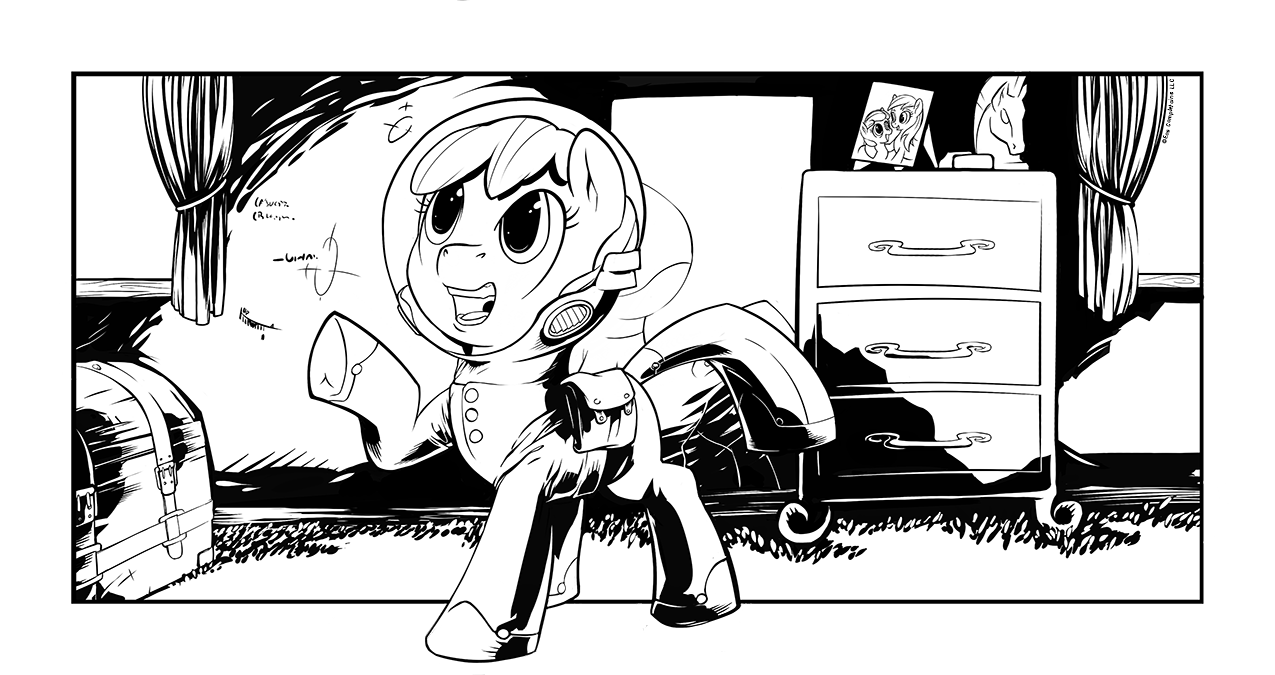
\includegraphics[width=\linewidth]{image01.png}

\begin{intro}
Do you believe in ghosts?
\end{intro}

``Please let us on! The shield is failing, there's no time!''

A long line of ponies waited impatiently in front of an air wagon, but there was no sign of the pegasus pilots. A green unicorn mare at the back of the crowd suddenly started screaming, desperately pushing ponies aside in a wild dash for the front.

``It's impossible! This can't be happening! Celestia abandoned us! Luna abandoned us! There's n-'' BLAM!

The panicked mare fell silent as her body hit the ground. All eyes turned to look at a soldier who racked a fresh shell into her riot shotgun. ``FORM A LINE AND WAIT YOUR TURN! THERE'S ROOM FOR EVERYPONY, TROUBLEMAKERS WILL BE MET WITH LETHAL FORCE!''

A little filly with a blond mane and pink coat was looking up at the sky towards Canterlot. A gigantic shiny bubble engulfed the whole mountaintop. The pink cloud trapped inside was the most incredible sight of her life, capturing her attention completely.

``Hey, you there!''

A unicorn medical officer dressed in a white uniform was distributing protective suits to the foals. She paused for a moment in front of the pink filly and gave her a worried look.

``Are you alone? Where are your parents?''

The foal smiled back at the officer. ``Mom is up there!'' She pointed a hoof at the force field surrounding Canterlot. The energy bubble seemed a lot thinner than ten minutes ago. ``She'll be back for dinner!''

The officer hesitated, before looking at the foal and trying to smile. ``Of course she will. What's your name, little one?''

``I'm Puppysmiles!'' cheered the filly, bouncing up and down on the spot.

``Yes\dots yes Puppy, alright\dots Now, listen to me carefully. I want you to take this suit and put it on. You must wear the suit and not take it off, do you understand?''

The filly looked at the yellow object with a puzzled expression, then at the white pony. ``Yes miss pretty pony! I like you!''

\emph{Dear Celestia, she's just a foal, she hasn't done anything wrong! This war is killing more than just ponies. This war is killing hope itself.} The unicorn levitated and unfolded the suit: it was lemon yellow, with several pockets on the legs and a couple of saddlebags on the sides. ``Ok, I need you to put your hooves in the holes for me. It's just like\dots like the pony pokey! Do you know the pony pokey?''

``Yush! \emph{You reach your right hoof in, you reach your right hoof out!}''

``Right, that's perfect! Now the tail\dots here, let me close it up and put this on your head\dots done!''

The mare put a round glassy helmet on Puppysmiles' head, then snapped shut a pair of locks on each side, finally sealing the small pony safely inside her radsuit.

``Woah! I look like a space pony! Like\dots like Captain Andromeda! Wooooosh!'' The foal started running and jumping in circles, giggling naively. The white mare simply sighed in relief and turned towards the next group with foals.

Puppysmiles was having a super duper great time. Everything began with those big fireworks like a super humongous surprise party and the castle was encased in a splendid bubble, like those she made with soap, just bigger\dots biggest\dots no, more! Biggester! And now everypony was in the streets for some sort of celebration. She prayed to her lucky star that mommy would come back home sooner today, so they could have fun together. The helmet and the space suit were just the icing on the cupcake; they were super cool and she was sure they made her look awesome\dots Right! What she needed now was a mirror! Without hesitation the filly rushed home.

The muffled street noise filtered into her mother's room. Puppysmiles stood in front of the dresser, examining her helmet from the inside. Strange lights and symbols danced across the glass. Objects in the room were ringed in green halos and as she looked at them in turn, writing appeared below\dots Too bad Puppy couldn't read. Her mom had barely taught her the basics.

``Buh\dots eh\dots duh.'' The filly frowned as she tried to construct the word. ``BED! Wow, I'm good!''

Satisfied, Puppy trotted downstairs, totally forgetting the mirror. Instead, she went for the fridge.

``Muffins!''

Puppy plucked one from the tray and went to take a bite. This immediately presented a problem: she couldn't get near it with that stupid helmet on\dots ``Do want but can't has\dots Bad helmet! How do I take you off?'' She grabbed the offending fishbowl between her hooves and wrestled with it for a full minute, but to no success. Panting, she sat down hard on her rump and decided to play her trump card.

``WAAAAAAaaaaahhhhhhh!''

Unnoticed by the whining Puppysmiles, a red symbol appeared on the visor. Her tantrum was cut short as a metallic voice began talking from within the suit.

``{\mt Status of the host -- panic}''

The filly derped for a moment. What was going on? Who was speaking?

``Wut?''

``{\mt Internal medical diagnostic initiated. Error. System rebooting. Estimated time, thirty seconds.}''

All those funny words were amusing but it didn't help with getting rid of the helmet. Puppysmiles was still upset.

``Go away stoopid talking space suit! I want muffins!''

``{\mt Reboot complete. Checking version. Initiating. Ten seconds to full operational status\dots eight\dots seven\dots}''

In that moment Puppysmiles heard a crescendo of voices from outside. A mounting roar as all the ponies in the city screamed in terror; it was as if Canterlot itself cried out one last time before the end, a desperate realization of the incoming doom.

``{\mt Five\dots Four\dots Three\dots}''

Suddenly, the world went pink. Looking out of the window the foal could see a shadow that grew darker and darker all over the place, as if a gigantic sugary pink cloud was falling on them. Oblivious to its meaning Puppy pressed her helmet against the glass of the window, curious as to what was going on outside.

``{\mt Two\dots System rebooted. Starting diagnostic routine. Warning. Primary healing talisman is not responding. Activating backup healing talisman. Starting diagnostic. Female. Foal. Earth pony variety.}''

Wow, this space suit was smart! It knew a lot of things! ``Hi, I'm Puppysmiles!''

A blanket of pink mist flooded the streets, muffling the sounds of the ponies it caught, their terrified screams being washed away as the cloud brought them death\dots or worse.

``{\mt Life support online. Temperature within parameters. Blood pressure within parameters. Warning. Radiation level above the average by three hundred percent. Minor radiation poisoning detected. Inoculating -Rad-X- inoculating -Rad Away- inoculating -Rad Away-.}''

Puppy sat in front of the window looking a bit puzzled at the mist leaking inside. She now wasn't sure of- ``YEOW! Stoopid space suit! Why you stung m-YEEEOW! STOP IT!''

``{\mt Warning. Hazardous agent detected. Analyzing. Pink agent, Littlehorn type. Lethal at a concentration exceeding 5\%.}''

Puppy giggled. ``Tee-hee, space suit says fancy words!''

``{\mt 1.8\%\dots 2.0\%\dots 2.2\%\dots Warning. Concentration of pink agent above safety limits. Evacuate the area immediately.}''

Puppy stared in amazement as the pink fog poured from the window and across the floor, she smiled as it streamed between her hooves. It was like candy floss\dots pink candy floss! Yay! Her mom hadn't let her eat it since she made herself sick last Nightmare Night.

``I feel funny\dots''

``{\mt Danger! Mutation detected! Concentration of 5.4\%. Danger! 6.0\%! Evacuate immediately! Contact Ministry of Peace for immediate help! Initiating transmission of distress signal. Scanning for emergency channel. Transmitting. Warning! Concentration at 7.5\%!}''

``Ugh\dots mommy\dots I don't feel very\dots can I stay\dots home\dots tomor\dots'' Everything became foggy for the foal; she felt like she was sweating a lot while at the same time she was freezing.

``{\mt Inoculating -Med X-. Inoculating -Healing potion-. Concentration at 12.1\%. Inoculating -Rad X-. Inoculating -Rad Away-. Concentration of pink agent at 16.0\%. Inoculating -Poison Antidote-. Inoculating -Healing potion-. Inoculating -Healing potion-. Concentration at 22.6\%. Inoculating -Healing potion-. Inoculating\dots}''

The ceaseless litany of the radsuit's medical systems continued as Puppy's legs gave out beneath her. Lying unconscious on the kitchen floor, the healing potions that coursed through her veins kept her alive. As the deadly pink agent slowly permeated the suit, it did its best to mitigate the worst of the effects. She did not die, but she didn't quite survive either.

``{\mt \dots Healing potion. Inoculating -Healing potion-. Inoculating -Healing potion-. Warning. Healing potion doses left: three. Concentration of pink agent at 35.0\%. Inoculating\dots}''

Like an abandoned doll, Puppysmiles slept as her suit sang its clinical chorus of programmed procedures. Hazardous atmosphere, suit compromised, medical supplies exhausted. She heard none of it as minutes flowed into hours, hours into days\dots

The filly simply lay there, on the floor. Wearing the noisiest medical suit ever, which kept stoically informing her that she was almost dead and she needed\dots practically everything.

Days became weeks, weeks became months as Puppy kept sleeping, frozen in that very last instant of life.

Months stacked up in seasons, and season gave way to years; the suit continuing to sing its lullaby of medical emergencies.

Year upon year the voice of the suit became lower and lower, starting to crackle. The transparent helmet covered in dust hid the tragedy of the world outside from the filly's face as she took her longest ever nap. Sealed inside her suit, tainted by the cloud, decades passed until they became a century, then two\dots

The house bore the years without a single repair; it was a good house, built by earth ponies in the old pony way: brick by brick, with a solid roof and strong foundations; but everything has to meet its end. It began as a little crack in the middle of the main roof beam during spring, growing larger and deeper with every rainstorm until the whole thing just resigned to old age.

Right on Puppysmiles' head.

\horizonline

\englishdaytimeplace{1}{5:00 P.M.}{Clover Leaf Terrace, suburb of Canterlot}

When the building collapsed it raised a cloud of dust and pink smoke that persisted for several minutes before everything went silent again. When the dust finally settled, from under the ruins came a tiny, muffled voice.

``Owie\dots''

Slowly a brick moved, followed by another, revealing something glinting in the rubble. A round glassy helmet popped up, followed by the yellow silhouette of a very small pony wearing a radsuit. There was a long crack in the helmet, but somehow the damage began to disappear as the pony finished freeing herself from the collapsed building.

``Mom?'' The filly resembled an astronaut taking her first steps on an alien world. ``What is this place? Where is everypony? Mom? MOOM!?''

Something felt wrong, beginning with the fact that she was still wearing that talking suit.

``MOOOM!''

``{\mt Bzzzt- FzZZzzZzt- line\dots rebooFZZZt necesszSzT!}''

``Shut up suit! Where's Mom? Where is my house? Where\dots am\dots'' The filly's words died in her throat as she looked up to see a familiar mountain, topped by a ruined but unmistakable castle. There was no doubt: this was Canterlot, her home.

``What\dots b-b-but\dots it's\dots all broken!''

``{\mt Fzzzt\dots critical failure\dots no living parFZZZTT! Requesting conffFFZZZTanual rebooting}''

``Yeah, whatever!'' the filly yelled, while still looking at the ruins of Canterlot looming above her, and all of a sudden she felt funny again. At first her sight became foggy, and she fell on her flank, her legs unable to support her. Puppysmiles grew weaker and weaker, feeling a terrible pain crawl from her hooves up to her spine. It was a new type of sensation: everything in her just seemed to stop working and the harder she tried to do anything, the more she felt trapped in her own body. The little filly tried to scream but her mouth wouldn't move. The only thing she could do was look at the empty street through a cloud of pain and a dusty helmet.

As she stood there, her focus shifted to a pile of strange dirty white stones. Their shape was unusual: long, thin, some curved, some straight. Now that she was paying attention, the foal realized that they were everywhere. The sight disturbed her slightly, but the sensation didn't last long: a green dot pulsed before her eyes, commanding her full attention.

``{\mt Reboot complete. Checking version. File not found. Starting emergency mode. Version 0.2\dots}''

``Ugh.'' Puppy tried to say something, but she was still completely paralyzed. The foal just stared at the weird lights in front of her eyes that turned from green to pink. Hey, good news at last! She loved pink, it was her favorite color!

``{\mt New components detected. Initializing matrix. Connecting.}''

A spark ran through the foal's body, from her nose to her tail, washing away that horrible sensation of paralyzing weakness. With some hesitation the filly tried raising a hoof. Finding no resistance, this encouraged her to try a few uncertain steps: it worked. It was as if the last five minutes had never happened. She just got better all of a sudden\dots go figure\dots

``Wow, that was weird\dots Now I just need to get this stoopid space suit off---''

``{\mt All systems operational. Starting diagnostic routine. Analyzing. Subject 001, Puppysmiles. Female. Foal. Earth pony variety. No vitals. Checking for errors in diagnostic equipment. No error found. Repeating diagnostic routine. Female. Foal. Earth pony variety. No vitals.}''

``What are whytles? I want whytles! Are they yummy!?''

``{\mt Launching Learning Program for Foals. Connecting to Ministry of Image for recent updates. Unable to establish communication bridge. Launching program from backup files. Please wait for installation to finish.}''

The filly started trotting around, moving toward the pile of old weathered stones and stopping to get a better look at them. The HUD in her helmet illuminated the heap, surrounding its silhouette with a pink halo.

``Curly cuh\dots oh\dots ruh\dots puh\dots ss\dots eh! Cor\dots corrupse!'' The filly jiggled, reading was fun! A second later, she frowned. ``What's a corrupse?''

``{\mt Corpse, noun. Remnants of a dead creature -- the more you know!}'' The metallic voice quickly answered the question.

``{\mt Dead? Like\dots dead dead dead?}''

``{\mt Searching synonyms for dead\dots Cadaverous. Deceased. Defunct. Departed. Done for. Erased. Expired. Extinct. Gone. Inanimate. Inert. Lifeless\dots}''

Puppy listened for the first part of the list, then poked a long white bone with a hoof. Her eyes pointed out something just too familiar in this skeleton.

``Uhm, mister voice\dots this corpse\dots what was it?''

``{\mt Analyzing\dots Pony. Adult female. Unicorn variety}''

The little foal shivered, or at least felt like shivering. Her eyes rose, looking down the street littered with bones everywhere. Skeletons of dead ponies, curled on themselves, lining against the walls, corralled in small groups as if they had tried to find safety in numbers. All dead. Everypony was dead.

``What\dots what happened? Mom? Where's Mom?'' Puppysmiles felt a cold sensation running down her spine. ``Mister Voice\dots where's Mom?''

``{\mt MoM, Ministry of Morale. Analyzing data. Connecting to Equestrian Cartography Onspark. Downloading data. Error, name matching failed. Searching for MoM broadcasting signal. Spritebot found. Establishing communication bridge\dots }''

Puppysmiles stopped following the voice after the first two or three sentences, now she was trying to find her home. Maybe her mother was there waiting for her!

``Why is everything different? Where is my house, where are all the pretty ponies?'' Glancing down the street she saw the rusted and battered remnants of the Pony Joe's Doughnut shop, confirming that this was the street where she lived. Her house must have been\dots ``B-B-But\dots'' She stood in front of the ruins she'd crawled out of just minutes ago, looking at them in disbelief.

``{\mt Query: broadcasting source. Broadcasting signal found. Location marker transmission in progress\dots}''

``If this is home\dots where's my mom?'' Puppy sat down and started to cry, or at least tried to; quite soon the foal realized that she was just bawling; no tears ran down her face and she didn't feel relieved at all. Now the filly was almost sure that something in her was wrong; she was going to ask the mechanical voice about that, but was interrupted.

``{\mt Ministry of Morale's locations added to map. Nearest MoM hub displayed on the navigator.}''

``You\dots you found my mom!?''

``{\mt Affirmative. MoM has been located. Nearest MoM hub outside Canterlot Ruins is set as new navigation priority.}''

``Uh\dots I\dots guess that's a yes?''

``{\mt Instructions: follow the pink arrow on the compass until destination is reached.}''

``Uh\dots thanks?'' The filly took some seconds to realize how great this thing was. That voice had just found her mom! She was going to see her mommy, everything was going to be all right! Who cared about the house, the dead ponies, the ruined castle or this stoopid\dots no wait! This super duper smart talking space suit was going to find her mom! The thought filled her with such glee that it pushed everything else from her mind. Who cared that she didn't feel hungry or tired or whatever, Mom would know why! She was going to find her mom, everything was going to be fine!

``YAY!''

\horizonline

\englishdaytimeplace{1}{8:30 P.M.}{Sunshine Plaza, outskirts of Canterlot}

``{\mt Warning. Vital parameters absent. Warning. Medical supplies exhausted. Warning. All emergency channels are mute. Warning\dots}''

\begin{song}
    Warning wrap up warning wrap uuup!
\end{song}

Puppysmiles was trotting down the streets of Canterlot's suburbs, singing her personal version of the greatest hit ever in all of Equestria, trying to match the suit's timing so that it seemed like a chorus\dots and no, it didn't work.

\begin{song}
    The medical supply's tired!
    
    warning wrap up warning wrap up!
    
    We'll soon need batteries!
\end{song}

``{\mt Negative. Energy supply is sufficient. Estimated lifetime of the spark before red level, one thousand and two hundreds years.}''

``Oh come on! Just sing and stop whining.''

``{\mt Negative. This is not whining. This is a warning. I can supply appropriate audio samples of whining.}''

``{\mt Warning for what? Everything will be all right as soon as we find my mom! She's the coolest pony ever!}''

``{\mt Negative. MoM is not a pony. It's an acronym for---}''

``Of course Mom's a pony\dots and she's not an\dots uh\dots an acrobat either!''

``{\mt Negative. It's Ministry of Morale.}''

Puppysmiles giggled. ``Silly mister suit, sticks and stones can break my bones, but words will never hurt me!'' She giggled again, ``Ministry of Morale, as if that has to do with anything\dots''

Puppy trotted the deserted roads, past the bombed out relics and ghosts of ponies long dead. As daylight faded into dusk, she found herself in a large city square before a statue of Princess Celestia. ``Wow, pretty princess Celestia\dots when I'm big I want to be a princess too!''

Puppy paced around the monument with curiosity, trying to find a way onto the statue's back. Having a ride on a gigantic marble Celestia seemed just too awesome to be a bad idea, but as she prepared to start her ascent, the suit interrupted.

``{\mt Warning. Hostile detected. Distance, twenty meters. Analyzing\dots}''

A red dot appeared on the compass beside her pink objective. Turning to face it she saw a pony watching her from the doorway of a post office. At last! Somepony else! What'shisname, Horse Tile? Tee-hee, that's funny name! The filly skipped towards him with her best winning smile.

``Hi mister Horse Tile! I'm Puppysmiles!''

``{\mt Warning. Hostile at six meters and closing.}''

``Oh, and this is Mister Voice! He lives in my space suit and whines all the time but he's super smart!''

The creature stared at Puppy with an empty, glowing gaze. He was a horribly disfigured earth pony; his mane was almost completely gone and skin peeled off his body in several places, revealing rotting meat and yellow bones.

``GWAAH\dots'' growled the ghoul, as he took a step towards her.

``Uhm\dots is something wrong with you, mister Horse?''

``{\mt Analysis complete. Creature: Canterlot feral ghoul. Threat level: lethal. Tactical retreat is advised.}''

Puppy stopped, transfixed by the ghoul's unwavering red glare, suddenly aware of the horror standing before her. The ghoul simply stood, and stared back.

``Iforgotsomethingveryimportantsorrygottagookbyebye!''

The foal turned and sprinted for her life, scrambling over bones and screaming like the scared little filly she was. ``AYEEEEEEEEEE!'' The ghoul watched her display until she disappeared from sight, then sauntered back into the post office.

After several blocks Puppy finally decided it was safe to slow down and catch her breath. She looked over her shoulder, hoping the monster had given up the chase. The street was empty. Lucky Puppy, she was best runner ever, maybe she could do a sonic rainboom without even flying? Was that possible? It would have been super cool for sure\dots ``Okay mister Voice\dots you're the egghead. Is that not-so-pretty-pony still chasing us?''

``{\mt Negative. Scanning shows no activity in the area.}''

``Super\dots now let me just catch some breath then\dots then\dots'' Puppy realized something strange. She was barely winded despite having just ran half a kilometer at full gallop, she had really only stopped because she felt she should be tired. This seemed a teeny tiny bit wrong and made Puppy recall all the warnings the suit kept giving her\dots maybe there was something that she needed to know.

``Uhm\dots mister Voice\dots am I ill?''

``{\mt Running diagnostic procedure. Please wait. Negative. The subject is not ill nor wounded or poisoned.'' Puppy felt relieved: the thing about not being hungry or tired was probably nothing unusual. Her mom was always awake after Puppy's bed time, she never got tired. Maybe she was growing up at last? Yush! Puppy was becoming a big pony like mom! ``Diagnosis complete: the subject is deceased.}''

``Diseased? You just told me I was all right!''

``{\mt Negative. I told you that you were not ill.}''

The filly frowned. ``Waaaait just a moment. I'm not ill, but I'm diseased?''

``{\mt Negative. You are deceased.}''

``But that's the same thing I said!''

``{\mt Negative. The word you are using is incor-}''

``Aw, just stop with this I say tomato you say tomahto thing! It was boring even when I was five! You don't want to tell me what's wrong? Fine! I don't want to know! Bleh!'' Puppy stuck her tongue out at the helmet HUD and again started to follow her pink compass heading. She barely noticed that the night had drawn in around her, she could still see her way as clear as day\dots Unknown to Puppy, her eyes now shone with a faint pink light.

\horizonline

\englishdaytimeplace{1}{10:00 P.M. }{Dead Hills, Wasteland}

As the yellow suited filly made her way out of the city, she found herself at the top of a long and winding road. As it stretched into the distance she saw it pass through a desolate landscape of scorched hills and dead forests with little sign of civilization in between. In the darkness Puppy slowed to a stop and looked around, confused.

``Hey, mister Voice\dots are you super duper sure that this way is okay? We're not heading anywhere near the mountain top\dots''

``{\mt Affirmative. Nearest likely-intact MoM hub is located in this direction, however it is not currently broadcasting. Other hubs are also located further down this route.}''

The little filly frowned for a moment and it seemed that some big gears were making a lot of noise in her head while she was trying to translate what the suit had just said. In the end, she just smiled. ``Okie dokie lokey\dots let's sing something then!''

\begin{song}
    There, is a place, where the grass is what's for dinner!
    
    Charmed, fun and wild, there must be something in the water!
\end{song}

In the wasteland, walking down the road making as much racket as she was is just asking for trouble. Within half an hour Puppy had attracted the attention of every potential aggressor in the area, though most of them were a bit wary of how to proceed.

``{\mt Warning. Several hostiles detected. Caution is advised.}''

``Wut? Mister Horse Tile again!?'' Puppy looked around in a frantic panic; she was sure that she lost him in town, how could he- BLAM!

Suddenly the filly fell on her rump as a stinging pain in her left hind leg made it buckle. The pain wasn't that bad but for some reason she couldn't get up.

``Owie\dots''

A group of three ponies were running in her direction, screaming and foaming like mad.

``You! I'm gonna eat your heart! GRAAAAH!''

``I want his helmet it's mine I saw it first it's mine it's MINE! He's not bleeding! Why isn't he bleeding? MAKE HIM BLEED!!''

``{\mt Warning. Breach in containment layer. Exposure to external elements unavoidable. Survival of subject not guaranteed. Self repairing magic activated.}''

The foal waved a hoof at the new arrivals. ``Hi pretty ponies! I'm Puppysmiles! Have you seen my mom? Oh, and watch out for the horseflies! They sting like crazy!''

Puppy just sat smiling at the three ponies, trying to behave and ignore the annoying sting on her leg. Stoopid insects. The trio of ponies rushing towards her showed no sign of slowing down. She frowned for a moment. ``Is something wrong?''

``Immobilize that bastard! Cut his fucking legs off, I want to see how he does as a snail!''

A large earth pony tackled Puppy to the ground, effectively burying her under his sheer bulk. The other two ponies split up: the unicorn kept his distance and trained a rifle at the foal's head, while the earth pony mare pinned Puppy's forelegs.

``Got you! Now hold still while I---''

``{\mt Warning. Pink agent, Littlehorn Type detected.}'' When the earth pony landed on Puppysmiles a thick pink cloud puffed out from the large bullet hole in the suit, right in his face. At first the pony looked annoyed, but this emotion was rapidly replaced by realization, fear, panic, terror, as finally his head started to melt.

``Aaaah! Help me! Help! PLEASE! AAAGH! KILLMEEEAAAGGK!''

The other two raiders stared in disbelief at the massive earth pony as his face melted and dripped from his skull like an ice cream on a hot summer's day. The earth pony mare looked at the filly inside the helmet. She seemed so small, so innocuous\dots she has big\dots pink\dots gleaming eyes\dots

``It's a ghoul! Back off! Back o-COUGH COUGH!'' The mare tried to flee but started coughing up blood. It was too late to run, she had already tasted the pink venom and without a healing potion she was just as dead as her companion.

The unicorn screamed in panic like a foal, threw the rifle against Puppy's helmet and then ran for his life. In the meantime the big male rolled from Puppy's back as liquefied brain leaked from his skull's orbits and splashed onto the asphalt. The female tried to run while choking on her own blood, managing to get about a hundred meters before collapsing.

``{\mt Warning. Breach in the containment layer. Exposure to external elements unavoidable. Survival of the subject is not guaranteed. Repairs in progress.}''

Puppy was reeling: shell-shocked by the big pony dying right in front of her\dots it was worse than a horror movie, mostly because this was real. What in Equestria could have done that? Melting a head with all the skin and the bones and\dots suddenly she realized. ``Mister Horse Tile! He had the same melted face! He killed them!'' and now she was next! No\dots no, no, no, no! That wasn't good, she had to get up and run away super fast. Rainbow Dash fast! Unfortunately her leg wasn't cooperating. She tried to get up and run but could barely manage a stagger, so stagger she did as fast as\dots uhm\dots let's say a crippled turtle.

``{\mt Repairs completed. Containment restored. Running medical diagnostic. Subject deceased.}''

``Don't you dare start that again! We're in a pinch here!''

``{\mt Negative. No immediate threats detected. Hostile count in the area: zero.}''

``Count? Mister Horse Tile is a noble pony?''

``{\mt Negative. The correct word is hostile. You are distorting the meaning of-}''

``What are you, a dictionary!? I'm tired of your fancy words!'' Puppy sighed with frustration. ``Look, there's a super evil zombie pony count after us. We have to get out of here before he finds us again!''

``{\mt Negative. There's a misunderstanding of Celestial pro---}''

``CUT. IT. OUT!'' As the anger grew inside Puppy her eyes began to burn. No really: they were literally producing brilliant pink flames! They were so bright that she could finally see herself reflected in the glass of the helmet, working like a mirror in the darkness. What Puppy saw was a terrible creature with mad, burning eyes: a soulless monster that scared her to the bone.

Speechless and completely lost in the vision, Puppy fell to the ground. She clutched the helmet between her hooves, closed her eyes and started to cry. There were no tears, but it was loud; a soul-felt wail that lasted for hours.

\horizonline

\englishdaytimeplace{2}{6:45 A.M. }{Dead Hills, Wasteland}

During the night several creatures had been lured by the sound, but none of them dared to approach the yellow filly; something about her unsettled them deeply. It was already morning by the time Puppy finally stopped crying. Slowly she lowered her hooves from the helmet and opened her eyes. The suit had gone mute since her little scene the previous night; now she was starting to feel a little lonely.

``Uh\dots mister Voice\dots are you there?''

``{\mt Affirmative. All systems are powered and ready.}''

``Ah\dots right\dots I\dots I just wanted to say that I'm sorry\dots I didn't mean to shout at you. I\dots''

``{\mt Warning. This program is not designed for socializing. The emergency mode only provides hardware support, voice command interpretation and basic survival advice.}''

``I\dots please\dots please, please, please, don't leave me alone! I'm sorry! Please take me to my mom!''

``{\mt Location MoM already set as priority navigation point.}''

Puppy hesitated for a moment, trying to understand what the voice was implying. ``Uhm\dots are you saying that we are still going to find mom together?''

``{\mt Affirmative. It is the set priority.}''

``YAY! I love you mister Voice!'' Puppy was suddenly interrupted by the sound of a manly metallic laugh, but it wasn't coming from inside her helmet. The filly looked around, trying to pinpoint the source, and found a spritebot fluctuating in the air behind her.

``Uh\dots hi? I'm Puppysmiles\dots'' After her last experience with newcomers she wasn't completely sure that the \emph{everypony is a welcome pony} approach was the best one, but she had been told to be nice and she didn't want to disappoint her mother.

The spritebot hovered for a few moments longer, then replied: ``Oh, hi Puppy\dots can I call you Puppy? You are quite an interesting encounter.''

Puppy smiled happily. A friend at last! ``Sure! Everypony calls me that. What's your name, buzzing eye?''

``I'm Watcher, pleased to meet you.''

The foal tilted her head. ``What are you watching?''

``Well, anything that I find interesting.''

``Wow, that must be a lot of things!''

The bot laughed for a moment. ``Well, yes, quite a lot\dots say, is that a fully functioning Mark VI Omni-Environmental Suit you are wearing?''

``Nope, it's a space suit! It's super cool and it also talks, but I can't get out of it.''

``Oh, and how did you get inside it?''

``A pretty pony put it on me yesterday.''

``Yesterday? Can I ask who that pony was?''

Puppy pondered for a moment. ``She had a pretty white vest and made me sing the Pony Pokey\dots it was all a bit crazy, she didn't tell me what her name was\dots''

``Crazy? Like what?''

The filly frowned, trying to remember the important details of the encounter. ``Well, there was this big bubble all around the castle and the streets were full of ponies and soldier ponies and then all that pink mist and-''

``Woah, slow down for a moment! Pink mist? Castle? Do you mean in Canterlot?''

``Yup! Well\dots not \emph{Canterlot} Canterlot\dots we live downhill, but it's still Canterlot, you know?''

``Yes I\dots I know\dots'' The voice hesitated. ``And\dots this happened yesterday?''

``Uh\dots maybe it was a couple days ago\dots yesterday I woke up and all the pretty ponies were gone and\dots ah\dots my house was gone too and\dots there were lots of corpse ponies and it was creepy\dots and a really ugly pony chased me but now it's okay because me and mister Voice are going to find my mom!''

The spritebot was silent for a long time; Puppy just kept smiling, waiting for her new friend to say something else. When the voice finally came back it sounded distant and somehow not so friendly.

``So, after the thing with the pink cloud, you went to sleep and you woke up the next day and everything was just\dots gone\dots''

``Eyup!''

``And\dots you've not been able to get out of the suit since then and\dots you haven't had to drink or eat or\dots go to the restroom?''

``Nopey mopey.'' The filly smiled. ``Mister Voice said it was because I was diseased but then he said no and then yes and we had this big argument about fancy words.''

``And\dots can I ask you where you are going right now?''

At last an easy question. ``Sure! I'm going to find my mom! Mister Voice found her and I'm following this super nice pink arrow! When I find her everything will be all right!''

``This\dots mister Voice\dots pointed you in that direction? Down this road?''

``Yes! Wow, mister Watcher, you are super curious, aren't you? You should be called mister Questioner!'' The filly giggled, the voice didn't say anything for almost a minute.

``Oh Celestia I\dots I can't\dots Listen, Puppy, I\dots''

``Yes?'' The filly's eyes grew bigger.

The voice went mute again for a long while. ``I'm sorry, I have to go. I\dots I wish you luck.''

``Sure! Good luck to you too! When I find my mom I'll tell her that you were nice to me! Bye bye!''

The spritebot gave a brief burst of static and began playing some music, floating away in the direction of Canterlot.

``Wow, music! He has music! Cool! Hey mister Voice, do we have music too?''

``{\mt Affirmative. I receive several radio signals. Some of them are meant for entertainment.}''

Fancy words again, Puppy frowned trying to translate that sentence. ``Uhm\dots this means we can has music?''

``{\mt Affirmative.}''

``Do it!''

After a few crackles of static the radio began playing. The little filly in yellow continued south, trotting merrily along the lonesome road.

\begin{song}
    What is this place

    filled with so many wonders?

    that I am now under\dots
\end{song}

~\vfill

\begin{engnote}
    LVL up\dots no wait, Puppy uses a monster template! does she get lvls? I think not.
\end{engnote}

\engprintstatus{5}{4}{5}{7}{4}{6}{9}


\chapter{Party Hard}

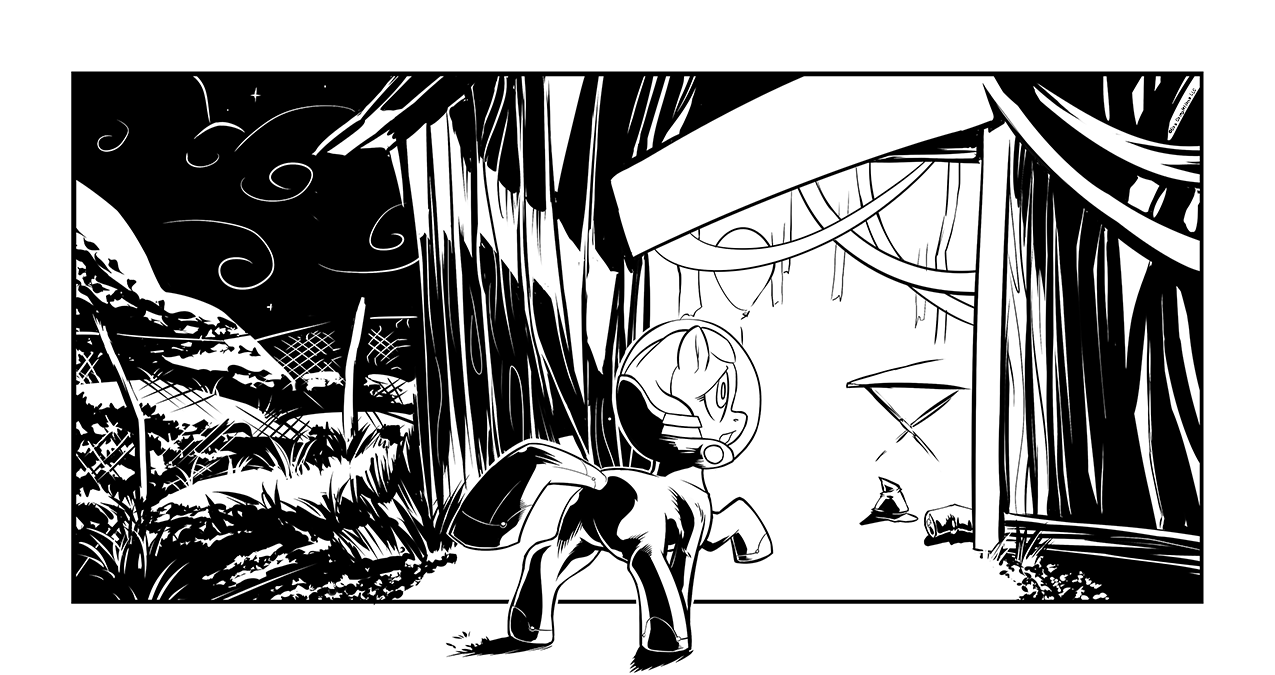
\includegraphics[width=0.9\linewidth]{image02.png}

\begin{intro}
No need to bring a gift, being there will be enough!
\end{intro}

\englishdaytimeplace{2}{4:00 P.M.}{Redtrotters Ridges, Big 52, N. Branch}

Usually, wearing a full environmental suit is not considered the cutting edge of Equestrian fashion, but anypony has to admit that it brings some neat advantages. First of all, if you were to survive a direct hit from a balefire bomb, you'd probably live long enough to die of thirst inside the suit before the radiation got you. The other good thing about being inside a hermetically sealed, radiation shielded suit is you'll never want for an umbrella or sunscreen again. And being lemon yellow, it's nearly impossible to go anywhere unnoticed unless, perhaps, you've been buried under an avalanche of lemons. Obviously there are moments in the Wasteland where stealth is a virtue.

As if Puppy even knew the meaning of the word.


\horizonline


``Hi! I'm Puppysmiles!'' She beamed at the two new ponies in front of her. Their uniforms, if they could be called that, resembled the trio from the other night's, but seemed cleaner and less ragged. One, a unicorn mare, scanned the road behind Puppy with her caravan shotgun, searching for what was to her an obvious ambush. Beside her, her earth pony partner kept a large spear levelled at Puppy. Had the foal been a wiser pony, the two mare's actions might have worried her.

The unicorn was the first to talk. ``What are you doing in Redtrotter territory, foal?''

``And what the hay is that weird suit?'' added the earth pony.

``I'm looking for my mom!'' Puppy replied enthusiastically, pointing a hoof more or less in the direction the road was going. ``She's that way!''

The two tribe ponies exchanged a glance before the unicorn spoke again. ``Okay, and what's your mother's name? Is she a Redtrotter?''

``What's a Redtrotter?''

The unicorn, her unease flaring into anger, prepared to go ballistic on Puppy. Sensing this, her partner stepped in. ``We are the Redtrotters. We control the Transequestrian Route 52 from here to Salt Cube City. If you have business on the Big 52 you do it through us. So, what's your mother's name?''

``My mommy is called Rainy Days! She's super cool and she always sings for me and she's a great cook too! She's the best pony ever and when I'm big I want to be like her!''

``Yeah, all right kid, I get the point,'' snapped the unicorn. ``I don't know a Rainy Days, so she's definitely not a Redtrotter. Are you alone? Who sent you here?''

``Mister Voice is with me!''

``Mister Voice?'' The unicorn warily surveyed the road again.

``Yeah! He lives in my space suit and sometimes we sing together but sometimes he gets grumpy but it's okay because he's helping me find Mom!''

\emph{``Right.''} The mare lowered her guard. ``Look, I'm sorry, but if you and your invisible friend want to pass through here, you need to pay the fee.''

``Ah, okie dokie? I have\dots'' Puppy started searching the many pockets of her suit. She had amassed a small hoard of junk in her short travel, mostly broken toys and things she thought were interesting. Maybe she had something these ponies would like. After all, \emph{you gotta share, you gotta care,} right?  ``What about this?''

Manipulating things without her teeth was quite a problem. She had to use her hooves instead. This task was only made more difficult by her bulky rubber boots, and the fact that she had to bend her leg at an awkward angle in order to reach into her saddlebags. ``Just a minute, I've almost got---no, uh.''

{\mt ``Assistance. The suit is equipped with a weak manipulation spell. Access your Inventory from the HUD and ask for the required item.''}

``Wut?''

The earth pony watched as Puppy mumbled to herself while fumbling out various useless junk from her saddlebags. The filly obviously couldn't pay. The spearmare looked at her friend and caught a meaningful glance. She sighed wistfully and after a brief internal prayer to the cruel gods of fate, plunged her spear into the foal's neck. Puppysmiles was so busy listening to the suit that she never saw it coming. She dropped to the ground like a sack of bricks, the earth pony letting her fall, silently cursing the Wasteland.

``You did her a favor. She wouldn't have lasted a day without her mother, and we can't afford to take her in. Better that we made it quick then let her get eaten by a manticore, or worse. You know what happens to foals around here,'' the unicorn trailed off with a sigh.

The earth pony noticed the troubled expression of her companion. ``Yeah. Poor Ridge Racer.''

The spearmare retrieved her weapon from the body. As she stepped back, pink smoke began to escape from the hole in the suit. The mare stared at the phenomenon, puzzled. ``Hey, Boney, what's that?''

The unicorn scratched her head with a hoof. ``You must have broken some talisman in the suit. It could be poisonous. Best to stay back.''

``We can't just leave her here, it doesn't feel right.'' The earth pony hesitated, trying to keep away from the pink smoke.

``After that funky little smoke show, I'm not going near her! The radroaches can take care of it. Come on, we still have a patrol to finish.''

With a final look at the fallen foal, the two mares trotted away, leaving the main road before climbing over a low ridge and out of sight. Time passed as the body of the filly in yellow lay alone in the middle of the road. A cold breeze picked up, rustling the bare trees. Despite the wind, the pink cloud that surrounded her did not seem to dissipate.


\horizonline

\englishdaytimeplace{2}{4:30 P.M.}{Redtrotters Ridges, Big 52, N. Branch}

The first sign that the lance had failed in its purpose was the automated speech of the suit coming back to life with a series crackles.

{\mt ``Initializing system. Checking version. Warning. Version number not corresponding. Starting in emergency mode. Version 0.2. Checking equipment status. All systems online. Major breach detected. Repair spells activated. Resuming last session. Loading personal data for subject 001: Puppysmiles. Subject deceased, condition stable. All clear.''}

Puppy's eyes began to blink for a moment inside the helmet, as if she had just awoken from a pleasant sleep. The foal yawned and a droplet of pink, glittering fluid fell from her mouth and onto the helmet of the suit, disappearing almost immediately as it was absorbed by the glass.

``Uhm, five more minutes, Mom.'' She turned around, still surrounded by the pink cloud that was now slowly fading.

{\mt ``Breach repaired. Subject insulated from external environment.''}

Lazily, Puppy got up and looked around. She frowned at the unfamiliar settings for a few moments before her memories came flooding back. ``Oh, right, Mom's not here. What was I doing before going to sleep?'' Puppy tried to scratch her head, but her hoof found the helmet on its way. She frowned again, then shrugged and continued to scratch the helmet thoughtfully.

{\mt ``Retrieving temporary memory. Query: last performed action before losing senses---negotiating passage.''}

``Negotiating what?''

{\mt ``Interacting with self-proclaimed Redtrotter ponies.''}

Fancy words again. ``Red-who?''

{\mt ``Talking with the pretty ponies.''}

At last, something comprehensible! ``Oh, right, pretty ponies! Now I remember! Ah, where have they gone?''

{\mt ``Location of Redtrotters unknown. Adding `Find the Redtrotter's' to the active mission list.''}

Puppy raised an eyebrow with a stumped expression. ``We have a to-do list? Since when?''

{\mt ``List initiated 23 hours ago. Objectives on the list: four.''}

``Wow, we have a lot of things to do! Four is a lot, right? What's on the list?''

{\mt ``Main objective: Reach MoM. Secondary objective: Get rid of space suit. Secondary objective: Confront Count Horse Tile or continue avoiding him. Secondary objective: Find the Redtrotters.''}

After listening to the list, the filly in yellow tapped her helmet with a hoof, a thoughtful expression on her muzzle. ``Think, think think. Muffins! No wait, that wasn't it.'' 

After several minutes of thinking, the foal finally nodded, a new resolve shining in her eyes. ``Okie dokie, play some music. Ah, the one with the chatty pony.'' Puppy trotted along the road, following the arrow and listening to the radio with a spring in her step.

The area surrounding Route 52 was a scorched wasteland dotted with rocks and ridges. It was hard to see very far because of the irregularity of the terrain. This normally would have been a problem, had Puppy any sense about her.

``Hey, Mister Voice, did you say something about taking stuff from my pockets?''

{\mt ``Affirmative. This suit is equipped with a weak manipulation spell.''}

``Uh, how does it work?''

{\mt ``Loading instructions. Selecting easy version for foals and Derpy. Name the object you need. If it is in your possession it will be put in front of you.''}

``Ah, muffins!'' A box of two hundred year old muffins floated in front of Puppy. She giggled. It looked so silly hovering in the air like that! ``Hey, this is fun! Sarsaparilla!'' A bottle of sarsaparilla replaced the muffins. ``Toy cart!'' This time a small toy cart in poor condition floated in front of the foal. ``Tee-hee! We need more stuff, I like this guessing game!''

{\mt ``Negative. This is not a guessing game. It is inventory management.''}

Puppy took a rock and put it in her pocket. ``A rock!'' The rock floated out of the pocket and listed lazily in front of her. ``Yay! It works!'' When it was put away again, the stone was labeled \emph{The Rock Of Destiny}, but since Puppy was not so good with reading, she didn't notice.

Trotting down the road, the filly kept asking for everything she had in her backpack, which really wasn't very much. She only owned four objects, but she planned on changing that soon. ``Oh, and we need more music!''

\begin{music}
		I can see that lone star from a thousand miles away
	
		Calling me back home, though I ventured far astray.
	
		When I see that beacon shining for me all alone,
	
		It calls me back to `Questria and my home!
\end{music}

\horizonline


\englishdaytimeplace{2}{7:00 P.M.}{Redtrotters camp, Big 52 N. Branch}

The Redtrotter's settlement was little more than a dirty bunch of half ruined shacks encompassed by a moat. Its barricade looked more like the result of a road crash between some old carts rather than a purposefully-built defence. Puppy was blissfully unaware of all this as she kept trotting toward the town, singing along with the radio until the road in front of her suddenly exploded into a shower of dust.

``Hey! I told you to STOP! RIGHT! THERE!''

Puppy looked toward the barricade and could see that there was a pony some fifty meters away. He was aiming a stocky gun at her. The filly sat down, waved a hoof and smiled. ``Hi! I'm Puppysmiles!''

The pony with the hunting rifle, who was peeking from behind the barricade, didn't seem very impressed. ``Okay, take that goldfish bowl off and show your face!''

``Uh, I'd totally do that if I could, but I'm stuck inside!'' Puppy pondered for a moment. ``Actually, it's on the to-do list!''

``Great, just great. Now, stand there where I can see you, and put down all of your weapons.''

``I don't think I have any weapons with me. I have a rock, does it count? I can throw it!'' She offered with enthusiasm.

The guard pony facehoofed. ``Hey, Doublesize, go and search her! You with the yellow suit, just stand there and behave!''

``Okie dokie lokie!'' Puppy smiled, but for some reason her answer startled the pony behind the barricade.

``Just say okay, don't try anything \emph{fun} and maybe nopony will get hurt! Do as I say now. Don't resist and let Doublesize do his work.''

A big, brown unicorn stallion approached Puppy, looking at the smiling filly through the glass of her helmet. The light was beginning to fade and now her eyes were just a bit pinkish, although it was hard to see thanks to all the equally pink lights coming from the helmet's HUD.

``Wow, that's a mighty fine radsuit you have there. Never seen one like this before.''

``Yush! It's super yellow and it's smart and it can do magics! Look! Look at this! A-hem. Muffins!'' The muffin box from before levitated in front of Puppy.

``Wow, integrated inventory management and lesser manipulation spells. This thing must cost a fortune. Where did you find it?''

``A pretty pony gave it to me in Canterlot!''

``So, you're from Canterlot?'' Doublesize gave a slight frown and shook his head.

She nodded proudly. ``Ah-huh!''

``The place with a big castle on the top of a mountain right at the beginning of the Big 52?'' 

``That's it!'' replied Puppy, smiling.

``Wow, that explains why you're wearing a full environmental suit at least. Okay, let's get back to business. Show me your pass.''

Puppysmiles stared blankly at the brown unicorn. ``My what?''

``You don't have a pass? Didn't you meet a patrol on the road coming here?''

``I met two pretty ponies. One was an earth pony like me and the other was a unir-unisc-unicron! They were super nice and super pretty!''

``Yes, yes, Rattling Bones and Frozen Soda,'' said Doublesize, cutting her short. ``Didn't they say anything about a passage fee?''

``Uh, I don't remember. We were talking for a bit, then they went away and left me alone and sleepy.''

The unicorn sighed and called for the pony at the barricade. ``Hey! The foal's clean, but it seems that Boney and Soda are giving out free passes today! The kid met them but she has no pass. What now?''

``Just take items from her that's worth the ticket and give her a pass!''

``Uh, okay.'' The earth pony stripped Puppy of everything she had but the rock and the suit. He tried to unlock even that, but the harness seemed to be sealed shut from the inside. ``Oh well, I guess it's just how things go. Sorry kid.'' He gave Puppy a flattened tin can with a red stain in the middle. ``Here you go, special discount for foals.''

``I'm telling my mom that you've been nice to me! Thank you mister pretty pony!''

``Oh, right, speaking of that, what's a foal in a rad suit doing all alone on the Big 52? This isn't a nice place.''

``I'm going to see my mom!'' Puppy took a look around as if she was trying to align herself with some invisible mark, then pointed a hoof toward a high ridge to the southeast. ``There! Okay gotta go bye bye!'' Without waiting for a response the foal merrily trotted away.

``But the only thing in that direction is the Carnival. Wait a second, kid! It's dangerous business going out there!'' Doublesize raised a hoof, but stopped himself. This was the wasteland and she wasn't family, so why bother? 

The filly in yellow wandered off the beaten path and explored among the rocks and the ridges. She found some sort of track, a winding trail running up and down the landscape just as if somepony had gone around dragging a couple of pointy sticks over the ground. Puppysmiles sniffed for a moment at the trails before ignoring them; for the foal climbing rocks and jumping from stone to stone was a super fun game; so, with \emph{a hop, a skip and a jump}, the evening became night as the foal ventured deeper and deeper into the wastes.


\horizonline

\englishdaytimeplace{2}{10:30 P.M.}{The Carnival, Wasteland}

A large barn stood at the bottom of a narrow valley, its once friendly coat of pink paint now faded and cracked. It was protected by a fence that ran all around the surrounding ridges, with automated turrets placed at fairly regular intervals. The building and the fence were in bad shape, and so were the turrets, but, despite their damage, several of the guns continued to slowly sweep side-to-side, guarding the perimeter.

{\mt ``Warning. Automated point defense turrets detected. Turrets are set on hostile mode. Threat level: medium.''}

The word hostile immediately put Puppy on alert. She stopped for a moment, looking around at her surroundings. ``The Count again? Where? That pony is persistent. Uhm, better safe than sorry, I guess.'' The little pony hid herself behind a rock and waited to see if Count Horse Tile was up to any mischief. ``Shush the music, Mister Voice, we're hiding.'' She held her breath and strained her ears to hear if somepony was moving.

{\mt ``Establishing communication bridge with the defense system. Exchanging protocol. Asking for clearance. Permission granted. The way is clear, please proceed.''}

``Shush, I said! There must be somepony here. It could be the Count! We have to be super sneaky.'' Puppy crawled out from cover and glanced over her shoulder in case somepony was creeping up behind her, before slowly moving toward the fence. The turrets almost immediately pointed in her direction, but their dots on the compass changed from red to pink and the guns returned to their default positions.

``Hey, Mister Voice, I told you to stop the music!''

{\mt ``Affirmative. The radio has been muted.''}

``So why do I keep hearing music?''

{\mt ``Sound source detected. The music is coming from inside the MoM building.''}

``From inside? Mom's inside that barn? With the music and everything else? Mom is throwing a party? YAY!'' Puppy instantly stopped hiding, got up on her hooves and ran downhill straight to the barn doors. When the filly arrived she bucked open the doors, jumped inside and yelled, ``SURPRISE!''

The barn's inside consisted of a single large hall with two open lofts, one right above the entrance and the other on the opposite, short side of the structure. The floor was made of flattened and pressed ground, covered sparsely with hay, and the walls were decorated with old streamers and garlands. From the ceiling hung some sorry-looking piñatas, a lot of limp, deflated balloons, and other old and half-destroyed decorations. The barn was sparsely lit by a couple of flickering lamps. The only thing that seemed to work properly were the speakers that were playing music at an almost deafening volume.

Right in the middle of the room there was a long table prepared for a party, with colored dishes and plastic glasses with names and everything else. There were plenty of guests sitting at the table: a bag of flour, a pile of rocks, a bucket filled with some unrecognizable liquid, and a chunk of dust, all of which wore a party hat. No less than a dozen lifeless, skeletal little ponies sat around the table, wearing festive party hats and staring blankly into empty plates. There were even a couple of corpses that looked more like mummies than skeletons. One of them might have passed for a very hungry pony. A large pile of white bones lurked in a far corner of the barn.

{\mt ``Warning. Mild radiation detected. Warning. Contaminating agent detected in the air. Analyzing. Nitrous Oxide. Threat level: negligible.''}

``Oh look, a new guest!'' A figure rose from its seat as the guest of honor. It was a pony with a staticky, fizzling voice that sounded like an old vinyl. In the dim light it looked like it was just a pink pony with an even pinker mane, but when it approached, Puppysmiles noticed that it was moving on a set of wheels, like it was wearing motorized roller skates. ``Well well well, look at you! I guess you're here for the masquerade! I'm super sorry to inform you that it was canceled, but you can keep the costume! It rocks!'' Usually, ponies moved their mouth when they spoke. Instead, this pony had an unmoving smile painted on her muzzle, and when she talked her eyes flashed with a creepy blue light.

``Uh, are you a robot pony?'' Puppy asked with some hesitation, remembering all the times her mommy had told her that she shouldn't point it out if other ponies looked weird.

``Well, yes I am! What a smart pony you are! I am a Recreational Pinkbot MK II prototype 03 and this is my birthday party! Want to join? I can free some seats. Some of the guests are getting a bit grumpy, and they don't participate very much.''

The robot rolled over to one of the skeletons, picked up the whole corpse and tossed it in the corner with the others, keeping just the party hat. ``Here you go, what's your name?'' asked the Pinkbot as it put a hat on top of Puppy's helmet.

``Uh, I'm Puppysmiles. I, uh, I'm looking for my mom. She's supposed to be somewhere in this place,'' Puppy said hesitantly.

``Fantastic! Maybe she will join us when she arrives! Now please, sit down. Would you like some cake?''

Puppysmiles wasn't in the mood for a party. She was supposed to find her mom in this place, not a stoopid birthday party! But maybe the robot pony could help her if she just played along for a bit. So the foal took her seat and looked around at the other guests.

They were creepy to say the least. The skulls pointed in her direction, the inanimate things dressed as guests, the two super skinny mummies and---

Wait a moment. A mummy was returning her glance? ``Please ‒\emph{giggle}‒ make this ‒\emph{giggle}‒ end.'' And she was speaking, too!

The little mummy was a unicorn foal with a pale yellow coat and an orange mane. She was losing hair and seemed very ill. The filly was giggling, but it wasn't a happy sound. It was like she couldn't help it. Her eyes were swollen, and fresh blood dripped from her nose, deepening the red streaks that ran down her muzzle. ``Please, ‒\emph{giggle}‒ I want to go home.'' She was muttering those words as if she had said them a million times, like if she said them enough she would wake up and this nightmare would be over.

Puppy felt a chill running down her spine. It passed from her shoulders to her tail and back up again. This place was wrong. She wanted to leave. \emph{But Mom could be here, she could be one of those\dots bone\dots heaps.}

A surge of panic threatened to overwhelm Puppy. This was just like that horror story where the super nice robot goes boing and starts hurting ponies! Way too many ponies had already suffered in this carnival of horrors and another wasn't far from sharing their fate! Not to mention that her mom could be on the list, especially if she was heading here. \emph{And what if she had already arrived? No, wait, the robot had said something about her not being there. But the robot could have lied! Could she lie? Who cares!} That pink thing was baked bads and Puppy didn't want to play her game anymore!

For a moment, Puppy's eyes met those of the giggling foal that sat at the table. That little pony missed her mom too. This barn was a bad place. ``Run away. Now. Go home.'' Puppy didn't stop looking into the other pony's eyes until the young unicorn nodded and tried to leave her seat. The Pinkbot moved to intercept her, but Puppysmiles intervened.

``Where's my mom?'' she asked, rising from her seat.

``We will go looking for your mom when the party is over, okie dokie? Would you like some sarsaparilla?'' The little unicorn filly staggered away, toward the entrance of the barn. ``Excuse me, the party is not finished yet, you can't leave!''

``Where is my mom?'' Puppy walked toward the pink pony droid, who immediately turned its attention back to her.

``Now, now, please behave, don't spoil the party. How about some Pin the Tail on the Pony?''

Puppysmiles eyes flared up with pink flames. ``Where is my mom? What did you do to her?''

``Error. Mom object not found. Please, do not get angry. I'm sure that your mommy will be here to pick you up very soon!'' The unicorn stopped for a moment, leaning against the door to keep herself upright. She could barely stand, and walking almost seemed like a torture. The Pinkbot rolled purposefully toward her. ``Stop right there! You can't leave without the permission of an adult!''

``Don't ignore me! She was supposed to be here! Stoopid robot! You are not going to hurt my mom or anypony else!'' Puppy snarled and lowered her head, assuming an aggressive stance. ``Rock,'' she muttered in a deep and menacing tone.

``Please don't use the S word. Suppressive measures ineffective. Subject immune to toxins. Brute force required. Activating sec---'' \emph{CLANK!}

``WHERE!'' Puppy's eyes were burning so bright that her helmet was filled with pink flames. The filly in yellow jumped at the robot's face, hitting it repeatedly with \emph{The Rock Of Destiny}.

``IS!'' With a feral snarl, Puppy wrapped her hooves around the robot's neck and headbutted it as hard as she could. The force of the blow created a spiderweb of cracks that ran across the helmet, but it also broke off the Pinkbot face plate, revealing the circuitry and mechanisms inside its head.

``MY!'' With one hoof Puppysmiles kept her hold on the robot's neck, while with the other she struck repeatedly at its exposed face. With each strike she tore cables and vital components from the machine, until at last she hit a talisman. The robot exploded as if it were filled with pink and yellow fireworks, launching Puppysmiles across the room.

\emph{``MOM!''} Puppy's flight ended rather abruptly as she collided with one of the automated turrets that had popped up after she had decided to get medieval on that robot. The impact severed a power cable, causing it to shut down with a plaintive whine. The remaining turrets locked on to her and unleashed a barrage of colorful beams that scorched Puppy's suit but were unable to penetrate it.

``Stop it! Tell me where my mom is!'' The filly charged a nearby turret head-on, slamming into it hard enough to knock it completely off target. The turret continued to fire wildly, now hitting the roof It proved to be far more effective against the barn's already weakened load bearing structures than it was on the magically resistant environmental suit. Puppy turned and finished it off with a buck that was so strong it tore the turret off its mount, silencing the machine, but not before the ceiling began to crack and fall apart.

``Mom! Mom where are you? \emph{MOM!}'' Ignoring the barn that was collapsing all around her, the foal ran toward the bones stacked in the corner. ``Mister Voice, do you see my mom? Where is she?''

{\mt ``Error. Destination reached. Ministry of Morale hub already found.''}

``What are you saying now? I want my mom! You said she was here!''

With one last, deep groan muffled by centuries of dust, the barn fell on Puppy's head, burying her alive.

As the first lights of dawn tried to pierce the ever-present curtain of cloud, a small emaciated unicorn filly crawled out of the defensive perimeter of the former MoM structure. The turrets lay still, having lost their power source. Even the music had fallen silent, its two hundred year lament finally over. Small patches of flame burned amongst the debris, failing to consume the remains, as rotten wood provided inadequate fuel.


\horizonline

\englishdaytimeplace{3}{9:15 A.M.}{The Carnival, Wasteland}

Even after its collapse, the cursed place was unable to find peace.

``I didn't ask you to find this Party of Horrors place, I told you to find my mom!'' said a muffled voice from under the ruins.

{\mt ``Negative. You asked,'' the suit launched an audio file with Puppy's voice, ``Mister Voice, Where is Mom?''}

``That's exactly what I'm saying!''

{\mt ``Affirmative. Ministry of Morale's nearest functioning hub was located and marked on the map. It was set as the primary objective and reached eleven hours ago before it was destroyed.''}

``Yeah, I remember that part, it exploded twice.''

{\mt ``Negative. It is impossible to explode twice. Major damages repaired. Systems fully functional and ready.''}

Puppysmiles went silent for several minutes, trying to think. Going harsh on Mister Voice was useless, mostly because there wasn't anything to hit, so she had to be smarter. She was a smart pony, right? That Pinkbot had said so, after all.

``Okie dokie lokie. It's useless to cry over spilled milk, I mean, under spilled barn. Mom wasn't here, but you said there are other places. So, what's next?''

% NOTE: force to break line

{\mt ``Warning. Despite the perfectly clear explanations, there is still a major mis-\\understan---''}
% {\mt ``Warning. Despite the perfectly clear explanations, there is still a major misunderstan---''}

``Aw, shut up! What's the next Mom's place we have to check?'' Really, Mr. Voice could be all work and no play at times. Dumb suit.

The suit went mute for a moment. If it had a more complex artificial intelligence it could have said something else, or at least felt frustrated, but this wasn't the case. This program was designed to be effective and to obey, so that was all it could do.

{\mt ``Next MoM location marked as primary objective. Location set as target on the compass.'' A new pink arrow appeared on her display as Puppy finished pulling herself free from the rubble. The filly jumped down from the ruins and shook herself, trying to get rid of the dust that coated her suit.}

``See? Everything is easier when you collaborate!''

{\mt ``Affirmative. Cooperation is magic.''}

A metallic chuckle interrupted the conversation and immediately caused Puppy to turn around. She was greeted by the sight of the buzzing spritebot she had met a few days prior.

``Oh it's you, Questioner. Hi!'' The filly smiled.

``It's Watcher. Anyhow, that was quite random, wasn't it?''

``What? You mean the party? Trust me, you didn't miss anything. Worst. Party. Ever. Everypony was dead. Uh, quite literally.''

``So, did you find your mom?''

``Nopey mopey.'' Puppy frowned for a moment, then she smiled again. ``But we have a lot of places to check, so it's okay! She must be somewhere, right?''

``Uhm, yes, I guess.'' He paused for a good while. ``And, may I ask where you are going now?''

``There!'' The filly pointed with her hoof, then added, ``This time I feel lucky!''

``So, you're going to check the next location of `Mom' in that direction?''

``Sure!''

The robot took another long pause before speaking. ``And you feel lucky about that?''

``Yup!''

``Oh well, at this point, why not. Very well. Puppy, I've got to go. Have a nice trip, and try to stay out of trouble.''

``Sure, Mister Questioner! Have a nice day!'' The spritebot turned and floated away, proudly broadcasting the March of the Parasprites as it did so.

``Oh, right! Mister Voice, put on some music!''


\begin{music}
		I don't want to set Equestria on fire
	
		I just want to start a flame in your heart
\end{music}

\horizonline

\englishdaytimeplace{3}{2:00 P.M.}{Redtrotters Flats, Big 52 N Branch}

Puppy was back on Route 52. She had left the rocky area behind her, the landscape ahead now mostly flat, dotted with the occasional ruin of an old farm. The silhouette of a big city began to emerge from the dusty air some kilometers in front of her. She could see skyscrapers in its center and a large half-collapsed dome to one side. Along the road there were carcasses of old carts, some were fast little racing carts while others were big, hulking cargo trucks. All of them shared the same fate; left alone to rust in the middle of nowhere.

``Hey! Hey you, wait!'' Puppy turned toward the pair of ponies that had called out to her.

The filly in yellow stopped to see who was coming and recognized the two mares from the other day. She smiled and waved a hoof. One of them stopped a little more than thirty meters away and readied an assault rifle. The other drew near, assuming a cautious stance but leaving her power lance sheathed.

``Ok, little Miss Miracle, stay put and nopony is going to get hurt.''

``Uhm, are we playing a game?''

The unicorn kept her rifle aimed at Puppy while the other pony answered. ``Yeah, something like that. Wanna play?''

``Great! Can I start? Huh? Huh? Huh?'' Puppy had already begun to jump in place like the hyperactive foal she was.

``Sure, why not? I'll ask you a question and you try to answer. If you don't reply, you lose. Got it?''

``Yay! Guessing game! I love-love-love guessing games! Ask me something, ask me anything!''

``Great. Question number one, how come you're still alive and unhurt after getting a power lance in the throat?''

``A what where?'' This one was hard. Puppy had no idea of what a power lance was but it seemed that there was some way to swallow it and to not get an owie by doing that. ``Uhm, pass?''

The two mares exchanged a glance again. ``Maybe she's just a retard?'' offered the earth pony. 

The unicorn sighed. ``Well, at least try asking a different question.''

``Okay, kid, so, why did you go to the Carnival?''

``You mean the old barn? Well, this stoopid Mister Voice told me that my mom was there. Guess what? She wasn't, and instead I found the worst party ever. There was this mad pink robot that wanted to hurt my mom and I got upset but the robot exploded and a strange thing started throwing nasty lights at me then I don't remember very well what was next but I think that the barn fell on my head. That happens to me a lot lately.'' Puppy stopped for a moment, pondering. ``I hope that skinny filly is safe.''

``Ridge Racer will live, and that's the only thing that keeps my friend from pulling the trigger.'' The earth pony took a long breath, ``So you resurrected, trotted all the way to the Carnival, destroyed that cursed place and saved Boney's sister, just by accident?''

``I, I don't remember doing all that, but if you say so.''

``And you were just looking for your mom the whole time.'' The mare said incredulously, raising an eyebrow.

``Yes, do you know where she is?''

``Yeah, she's a retard.'' The earth pony facehoofed while the unicorn behind her let out a hearty chuckle.

After a short laugh, the unicorn's expression became more serious. ``But she saved my family. I'm in debt to her.''

``So, what now, Boney?'' asked the earth pony.

``I don't know.'' Rattling Bones lowered the rifle and approached Puppysmiles, who gave her a grin. Somehow that enthusiasm and innocence stole a little smile from the hardened unicorn, and she placed a hoof atop Puppy's glass helmet.

``I'm not sure if you are good or bad news, but I owe you one, so, thanks.'' Rattling Bones took a rectangular scrap of metal with a white half-eaten apple painted on it, offering the object to the filly in yellow. ``Here, take this. It's a pass. If you're going to Salt Cube City, show it to the guards and they'll let you inside. Understood?''

Puppy eyes widened with glee as she stared at the gift. ``Wow, thanks! A present! I love presents! Thank you super much miss pretty pony!''

The unicorn continued. ``You put an end to a nightmare for our entire tribe and gave me back the only thing I cared for. I hope you'll find what you're looking for, little ghost.''

``D'aaaaaw, aren't you guys cute?'' mocked the earth pony mare.

``Oh, just shut up and let's keep moving, Soda. We have a patrol to finish.''

``Hey, are you crying, Boney?''

``Aw, just shut up! And don't you dare laugh or tell this story to anypony!''

``Guess what? Now I feel sorry for killing her.''

The two ponies left, heading in the opposite direction of the pink arrow. Puppy watched them trotting away and waved her hoof as they disappeared behind a ridge.

``I like pretty ponies, they are pretty!'' Puppy smiled, before setting off in the direction of the big city.

``Hey Mister Voice, can I ask you something?''

{\mt ``Affirmative. Please state your request.''}

``When we find my mom, are you going away? I mean, I don't want you to go away.''

{\mt ``Negative. As an effect of the Littlehorn Agent, this piece of equipment is irremediably fused with you.''}

``Uhm, this means that we are together forever? I can keep you with me when we find Mom?''

{\mt ``Affirmative.''}

Puppy smiled, listening as always only to the part of the explanation that she wanted to hear.

``All right, Mister Voice. You already know what we need to do now, don't you?''

{\mt ``Affirmative. Analyzing the previous interactions, your request is predictable with 95\% accuracy.'' The radio began playing music and Puppysmiles started to sing along.}

There was still a lot of road to trot, and she was by herself as always, but Puppysmiles was a filly on a mission, and she had that kind of stubbornness that can only come from ignorance. Besides, she wasn't really alone. She had one friend that she was well aware of and maybe a couple that she didn't even suspect.

\begin{music}
		You and me together will be,
	
		Forever you'll see,
	
		We two can be good company,
	
		You and me
	
		Yes together we two\dots
\end{music}

~\vfill

\begin{engnote}
	Level up. I think we already discussed this.

	Negative. Level up is mandatory in FoE canon.

	Okay okay, geeze, I can understand Puppy's frustration! Okay then.

	Quest perk added: leveling is mandatory---now you can gain levels! Yay!
\end{engnote}




\chapter{The Lost Herd}

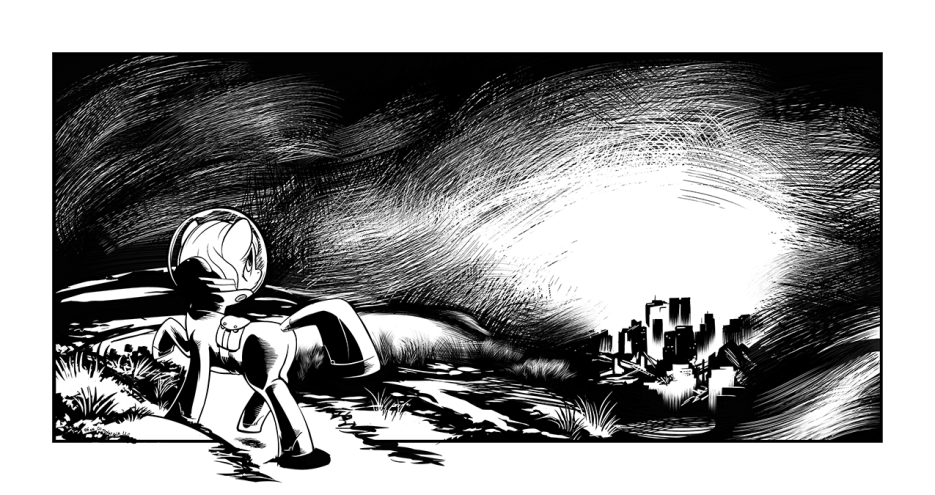
\includegraphics[width=0.9\linewidth]{image03.png}

\begin{intro}
Once upon a time, in the dying land of Equestria\dots
\end{intro}


\rtpr{``Good evening fillies and gentlecolts, this is Lonesome Pony speaking, and you're tuned to Radio 52. All the news you need to hear about Big 52 and nothing else! Well, almost nothing. In fact, it seems that now the biggest radio station in Equestria is broadcasting through all of the Wasteland. Some saint went down to Fillydelphia on behalf of DJ PON-3 and bucked the transmitter till it worked again. So hooray for those guys at Tenpony Tower, they took over the world!''}

Boisterous music played for a few seconds.

\rtpr{``Heh. That's everything from the big dogs, now back to the local news. Hey little ponies, are you afraid of ghosts? Maybe you should be. Do you remember the story of the Carnival? Don't worry if you don't. Good ol' L.P.'s going to give a quick recap for those that didn't do their homework.''}

\rtpr{``Far away on the north end of the Big 52 there lies a solitary barn. The Redtrotters call it `The Carnival.' It's a cursed relic from a long lost age, but unlike a lot of its siblings it never went to sleep. Once a year since before my grandpa could remember, a ghost would leave the building and lurk in the hills nearby, inviting everypony to its party and looking for company. When the next morning came, a foal was gone. No matter what, nopony ever returned. Approaching the Carnival was suicide thanks to the laser turrets that defended the place, but if you did succeed in getting close enough without being shot, you could hear music coming from the cursed barn, all day and all night long. A permanent party of horrors.''}

\rtpr{``Well, my little ponies, it seems that somepony just yelled 'I ain't afraid of no ghosts!', rushed inside the barn with the party in full swing and literally blew the roof off that whole place. No more foalnapping ghosts for the Redtrotters! I tried to gather some information about this benefactor, but what I got was a bit messy. Apparently, the one who did it some sort of ghost itself---a filly wearing a yellow radsuit and rising from death out of a pink cloud. Well, Yellow Ghost, nice work. One problem solved, nine-hundred-ninety-nine to go. Oh, and did I mention that this year's victim made it safely home? Celestia bless our souls! And now back to good old Pony Marcus!''}

\begin{music}
		I can see that lone star from a thousand miles away,
	
		Calling me back home, though I've ventured far away.
	
		When I see that beacon shining for me all along,
	
		It calls me to Equestria and a home!
\end{music}

\horizonline

\englishdaytimeplace{4}{00:30 A.M.}{Salt Cube Flats, Big 52 N Branch}

Puppy trotted along Route 52, heading south. The big city had grown from a silhouette on the horizon into a large, sprawling mass just a few kilometers in front of her. The foal had trotted all day long, and now the light was fading into darkness. Her eyes began to turn bright pink, shining in the night while she walked down the road. Without the daylight it was possible to see a green glow around the dome of Salt Cube City, while the bigger skyscrapers of Downtown were lit with sparse fires. The largest part of the city simply faded into the darkness of an ever-clouded night sky.

Around midnight, the filly in yellow spotted a small caravan heading in her direction from the south. There were about half a dozen ponies, and they had some sort strange two-headed cows with them. Puppy sat down in surprise, and waited for them to draw near. The caravan guards spotted the foal soon afterwards, being that she was a light source sitting by herself in the middle of the road. Needless to say, the guards were already on edge.

A large buck wearing a light combat saddle mumbled to another. ``What do you think, could it be that 'ghost' from the news?''

The leader of the guards, an earth pony mare with a big revolver, shrugged. Raising a hoof, she made the caravan stop. ``Dunno, but I'm not taking any chances. Let's move. Two on the sides, two here. I'm trying a diplomatic approach. Cover me or you can forget your pay.''

Two of the guards detached from the caravan and left the road, circling Puppysmiles, one on each side of her. Meanwhile, the leader ran ahead while the caravan with the remaining two guards kept their distance. The sight of the filly was quite an eerie one. The creepiness of the small yellow silhouette, which had a glowing pink light coming from its glassy helmet, was already a perfectly valid argument for opening fire. The leader of the guards approached the creature with caution, hoping that the other two guards were fast enough on the trigger in case of complications.

``Hi! I'm Puppysmiles!'' The foal raised a hoof, waving to the guard leader. Well, at least it didn't seem hostile.

In the Wasteland Survival Guide, there's a sentence that dwarfs all others when it comes to the sheer number of iterations: \emph{better safe than sorry.} Not seeming hostile didn't mean it was safe. ``Okay, now don't move, and tell me what you are and why I shouldn't transform you into fertilizer.''

Puppy giggled. Fancy words always made her giggle. ``Tee-hee, pretty pony is funny! I'm not Forty Liza, I'm Puppysmiles! What's your name?''

The guard leader hesitated for a moment. Was this foal simply retarded, or was it all part of some well-planned trap? The whole situation just smelled wrong. ``Yeah, I'm Solid Slug. Are you alone?'' Without waiting for an answer, the guard gestured to the two on her sides to check the surrounding area.

``Nopey mopey, I'm with Mister Voice! He's super smart or super stoopid, it depends. But for sure, he knows where my mom is!''

``And where is this `Mister Voice' now?''

``Inside the space suit! See all the lights and the pretty dots? He makes them appear!'' Okay, there was a nine out of ten chance that she was just a retard.

Solid Slug took a better look at the suit's helmet, trying to ignore Puppy's brightly shining eyes. There was an active HUD, quite similar to the one used in some models of battle saddles. Upon closer examination, the harness seemed like a very expensive piece of equipment. Solid wondered how a foal could ever find something like that, but the pink light emanating from the suit gave her the feeling that there was more to the situation. Solid Slug had been in the business for a whole lot longer than most caravan guards, and had picked up more than a thing or two about the Wasteland in all that time.

``Say, are you from Canterlot by any chance?''

``Yush! My house is, ah, was just under the mountain in Clover Leaf Terrace, but the other day it went down, so now I'm looking for my mom. She wasn't at the old barn, but Mister Voice says that there is another place in that big town so I'm going there now!'' Puppy pointed a hoof somewhere southward.

Solid Slug nodded a couple of times while listening, raised a hoof and gestured to the caravan. After some preparations the carts started moving again. ``Wow, you chat a lot, don't you? Lonesome Pony was speaking about your exploit at the Carnival.''

``My what? You mean the old barn? I didn't explode there, it was the barn that exploded, silly filly.'' Puppysmiles giggled. ``That Pinkbot was totally a baked bad! At first it was really creepy, but I'm a brave pony!''

Solid Slug scratched her head, trying futilely to follow Puppy's chattering. ``Uh, yeah, that's great. I'd stay here and chat for ages but we have to keep moving. If you're going to Salt Cube City, the ghoul community is at the Dome. I think they call it the Glow. Don't wander too much in Downtown, they don't like your kind. Oh, and, well, good luck, little ghost.'' When the caravan arrived the other ponies of the group sneaked curious looks at Puppy, but Solid Slug whispered to a purple unicorn with a red mane, and they simply kept moving. The filly in yellow stared with amazement at the brahmins and waved a hoof to the pretty ponies as they disappeared into the night. Once she was on her own again the foal trotted away, heading south along the Route.


\horizonline

\englishdaytimeplace{4}{11:30 A.M.}{Downtown, Salt Cube City}

The gate was a simple barricade built from sandbags and salvaged metal plates. On a wooden platform, a pony with metal barding operated a chaingun, while two other guards checked every pony that wanted to get into Salt Cube City. One last unicorn wearing an officer's uniform sat inside a small metal structure making notes in a register.

It was almost noon, but the traffic on the north end of downtown was as dead as the Wasteland. This time Puppysmiles was ready. She had that metal thing with the painted apple and showed it to the guards. One of the armored ponies approached her while the others kept their weapons ready.

``Let's see. Yes, this is a valid pass. Now, what's your name and business here?''

``I'm Puppysmiles! What's your name mister pretty pony?''

The guard raised the visor of his helmet, giving Puppy an annoyed look. ``Corporal Farsight. Now, what's your business in Salt Cube City, kid?''

``Oh, I know this one! I'm looking for my mom! She's somewhere in that direction!'' Puppy pointed her hoof toward a cluster of ruined buildings and the guard sighed.

``Very well, I guess that's enough. Just another question---why are you wearing a full environmental suit?''

``Oh, this one? I'm stuck inside it, but that's okay because Mister Voice lives in the space suit too and he's helping me with my mission.'' She lowered her voice, whispering to Farsight, ``He's not very good with that, but don't tell him. He's quite grumpy.''

The guard lowered his visor again and shrugged. ``As long as you're not going to blow a megaspell in Downtown, you can dress as you like. Welcome to Salt Cube City, kid.'' Puppy trotted beyond the roadblock, but Farsight called her back one last time. ``Oh, and don't go anywhere near the Dome. There are feral ghouls in the area, and it's heavily irradiated.''

``Okie dokie lokie! Bye bye mister guard Farsight!'' Puppy trotted merrily toward the big skyscrapers at the bottom of the boulevard, although the pink arrow pointed in a different direction.

Downtown was a typical trade hub along the Big 52. There were guards that kept ponies from killing each other and a couple dozen tents with signs of the different trading companies operating in the area, like the Water Herders or the Bullet Gallopers. There were even freelance traders and some trading posts from the nearest tribes. The open market was placed in the streets, but the real Downtown consisted of the four skyscrapers that still stood in the middle of the settlement. Salt Cube City had been the target of a single megaspell during the war, and the missile vector that should have delivered it malfunctioned. The warhead hit the Salt Cube Dome in the city periphery, piercing the roof and exploding at ground level. The massive structure of the Dome had shielded the surrounding area from the worst effects of the direct hit, but not from the fallout. During the successive two centuries, the most weathered buildings surrendered one by one to the ravages of time, but the four biggest and least-damaged skyscrapers survived and still stood in the middle of the city.

The four towers were the symbols of power in Salt Cube City. Two of them were each the main hub of a trading company, while the third was the headquarters of the Hired Hooves, a powerful mercenary company. The last building was the smallest one and housed the White Apples, the original tribe that inhabited the city. They were formally the real proprietors of the whole town and got a share of all the commerce going on in the place. The White Apples were also the main breeding ground for the Hired Hooves, mostly consisting of the families of ponies that worked for the mercenary company.

Puppy stood in front of a small tent marked with a red splash, the symbol of the Redtrotters. The shop sported a vast array of melee weapons and light armor on the shelves. A mare with an old cowboy hat was sitting on an ammunition box just in the middle of the exhibition.

``Hey, nice dress, little one. Say, are you from the north?'' The mare smiled at Puppy and lifted her hat with a hoof, revealing a horn on her forehead. The cutie mark on her flank depicted a basket ball.

``Hi! I'm Puppysmiles!'' She waved a hoof and trotted toward the mare. ``I'm from there.'' Puppy pointed at the street outside the tent.

``I'm Play Maker. I think that Lonesome Pony mentioned something about you last night.''

``Uhm, you mean the chatty pony on the music channel?'' Puppy scratched her helmet with a thoughtful expression. ``Last time he was speaking of the importance of drinking pure water.''

``No, no, I mean the news about the Yellow Ghost. Uh, maybe there's more than just one pony wearing a radsuit around. Anyhow, what do you need?''

Puppysmiles frowned. ``Why is everypony calling me a ghost?''

Play Maker smiled. ``So it's you after all, I knew it!'' The unicorn tapped her chin for a moment. ``Say, aren't you a bit too young to destroy a cursed barn? Actually, aren't you a bit too young to go around on your own? Are you a Crusader?''

``Nopey mopey. I'm looking for my mom, and I'm not alone! I have Mister Voice with me.''

``Your mom? Maybe I can help you: a lot of ponies visit Downtown every day. What's your mom's name? What's her cutie mark?''

Puppy smiled widely. ``Oh, her name is Rainy Days, she's purple and has an orange mane and her cutie mark is a cloud with raindrops! Have you seen her? Mister Voice says that she's somewhere in this place! That way!'' Puppy pointed her hoof again in the direction of some destroyed buildings.

Play Maker shook her head. ``I'm sorry, kid. Can't remember a pony with that palette or cutie mark, and the name doesn't ring a bell.'' She looked in the direction that Puppy was pointing and frowned. ``That way, you say? That can't be good. That's the radioactive area. The only standing building in that direction is the Dome, and trust me, you don't want to go anywhere near the Dome.''

``The Dome? What's that?''

``It's a place filled with feral ghouls and other horrors. It's highly radioactive, but maybe that's not a problem since you're wearing a radsuit. The real problem is the inhabitants: a small community of fanatical religious ghouls live there, but they're on the brink of madness. In fact, some of their 'siblings' went mad and attacked the caravans heading here. There's quite a situation now, and the White Apples are looking for a way to get rid of those rot-heads. They blast any ghoul that shows his face outside, but they can't go in and finish the job. The whole place is a deathtrap if you're not immune to radiation, so they reached a stalemate.''

Puppysmiles frowned. ``What's a ghoul?''

``You're kidding me! You don't know what a ghoul is?'' Play Maker stared at the blank expression on Puppy's face and sighed. ``No, you're not kidding.'' She shook her head. ``A ghoul is a pony that was poisoned by radiation a long time ago, when the megaspells hit. Instead of dying they were transformed into---I'm not sure what they are. The living dead? Maybe some sort of zombie? Anyhow, many of them went crazy because of that mutation and became feral ghouls---aggressive creatures that attack and try to eat everypony they see. Others retained their sanity and became immortal, but were disfigured by the mutation. Their manes fell out, their hides burned away, and their flesh began to blister and rot. Every ghoul looks like a decomposing corpse, but somehow they remain alive. The problem is that sooner or later every ghoul goes `boing' in the head and swaps their current diet for a meatier one.''

Puppy frowned. The unicorn could see fear and realization in her eyes. ``Miss Play Maker? Um, if my mom is really where Mister Voice says, will she be okay?''

``I---'' She lowered her hat, hiding her eyes from Puppy. ``I don't know, little ghost, but the Dome is a dangerous place. I hope you're not going there after what I told you.''

Puppy stood on her hooves with renewed determination in her eyes. ``I have to go! My mom could be there, and she could be in danger!''

Play Maker immediately realized that she'd never be able to talk her out of this suicide mission. ``You're not family, so I can't tell you what to do and what not to, but please listen to my advice. Go to that tower, the one with the big white apple on the sign. Tell the pony at the entrance that you want to enroll for a scout mission into the Dome. They'll give you some equipment and maybe a weapon. You have a radsuit, and they're so desperate that they'll accept anypony that they think could at least stand a chance.''

Puppy smiled. ``Okie dokie lokie! Hang on, Mom, I'm coming to rescue you!'' The foal galloped out of the tent and eagerly rushed to White Apple Tower.


\horizonline

\englishdaytimeplace{4}{2:00 P.M.}{Salt Cube Dome, Salt Cube City}

{\mt ``Warning. Mild radiation detected. Threat level: negligible.''}

The Dome was a humongous elliptical structure that had once served as an expo center where a large number of events could be hosted at the same time. A gigantic, globular roof once covered the building, but now it was almost completely destroyed, leaving only the external walls still adorned with columns and arches that made the structure vaguely resemble an oversized coliseum.

A boulevard headed right to the main entrance of the Dome, a monumental arch that led into a hall where the huge remains of a marble statue littered a floor that was once made of polished stone tiles. Now, it was mostly a carpet of rubble. Puppy stood in front of the archway, looking at the pink arrow on the compass.

``Okie dokie Mister Voice, what are we doing now exactly?''

{\mt ``Ministry of Morale hub reached. Primary objective attained.''}

``Yes, I know that we are here. I'm asking what's next. What are we supposed to do here?''

{\mt ``Secondary objective: investigate the ghouls and/or get rid of them. Warning. Mild radiation detected. Threat level: negligible.''}

``So, we find these ghouls, ask them where is Mom and then we try to make them go away?''

{\mt ``Affirmative. This is one possible approach.''}

``Great, I love having a plan. Let's do it.'' Puppy stepped into the hall and yelled, ``HEY, GHOULIE PONIES!'' It echoed several times into the large structure. She didn't seem to get any answer, so the filly in yellow trotted toward a large staircase at the bottom of the entrance hall.

{\mt ``Warning. Heavy radiation detected. Threat level: negligible.''}

``Hey, I think I've seen somepony moving behind that statue! Hey you, wait!'' Puppy galloped in the direction of a shadow that was hiding behind the pedestal of another broken marble monument. As the foal reached the hiding pony, she slowed to a trot and called out to him or her. ``Hi, I'm Puppysmiles! Have you seen my‒''

That pony! It was him---Count Horse Tile! He was right in front of her, even uglier than she could remember and somehow a lot creepier.

{\mt ``Warning. Hostile detected. Feral Ghoul. Distance: two meters. Threat level: low.'' The creature was looking at Puppy's face, drooling a yellowish goo from its mouth. It seemed oddly uncertain about its next move.}

Puppy stepped back, terrified by the macabre sight. ``W-why are you still coming after me? Leave me be! Go away!''

The creature growled and lowered its head, so Puppy turned on herself and galloped away as fast as she could.

Alas, it wasn't fast enough.

The feral creature jumped on her, foaming and biting, aiming for Puppy's head. The helmet was designed to endure punishment, so the first assault of the raging beast simply hurt Puppy's innocence. The sight and sound of a mouthful of rotting, jagged teeth scraping against her helmet was enough to paralyze her with fear.

``EEEEEEEEEEEK!'' Puppy reacted on pure instinct. She tried bucking the ghoul away, but it was a lot heavier than she was, and it pinned her on the ground with its weight. ``Rock! ROCK! NOW!'' She didn't stop screaming as she grabbed \emph{The Rock Of Destiny} with both hooves and started hitting the monster repeatedly. ``Stop moving! STOP MOVING NOW!''

A couple of minutes later, Puppy was still beating the brown slimy pulp that was once a pony's head. The scratches on her helmet and some minor bruises on the fabric were already gone thanks to the self-repair spells built into the suit. Slowly, the beating simmered down until it stopped completely. The ghoul was positively immobile and Puppy needed to catch her breath. It had been terrible, but at last the dark shadow of Count Horse Tile was gone! No more hiding or running away. The monster was stopped once and for all, his reign of terror extinguished! At last Puppy felt relieved, until she raised her eyes from the dead ghoul.

And finally noticed the three other ghouls that were looking at her with empty eyes and drooling mouths.

{\mt ``Warning. Three hostiles incoming. Nearest target: twelve meters.''}

``Hey, Mister Voice. What is a miss under---uh---static?''

{\mt ``Misunderstanding. The act of giving the wrong meaning to a word or sentence, creating confusion. The more you know!''}

Puppy nodded slowly while the three ghouls looked in her direction from the end of the hall. ``Good. What is exactly a Horse Tile Count?''

{\mt ``Hostile count. Number of enemies or ill-intentioned creatures in sensor range. Actual hostile count: three. Feral ghouls. Threat level: moderate.''}

Puppy sighed, threw \emph{The Rock Of Destiny} at the ghouls, and charged. The ghouls did the same thing from the other end of the hall.


\horizonline

\englishdaytimeplace{4}{2:30 P.M.}{Salt Cube Dome, Salt Cube City}

{\mt ``Warning. Several breaches in the containment suit. Warning. Littlehorn Agent detected. Warning. Compass malfunctioning. Warning. Inventory management spell temporary offline. Warning. Energy crystal cells damaged. Emergency cells on 29.06\%. Warning. Deadly radiation level detected. Threat level: negligible. Subject deceased, condition stable. All clear.''}

Puppy stood in the middle of a scene of mayhem, decorated with goo and rotten flesh. The bodies of three ghouls lay scattered on the ground with their heads missing. The whole fight had taken a while and been very messy, since the ghouls kept regenerating because of the radiation in the area. However, Puppy had also been regenerating because of the Pink Agent and her radsuit's enchantments. In the end, the foal's dedication at aiming only for their heads won out over the brainless biting and bucking of the ghoul trio, but in the process she had been beaten like a bucking bag. Her flanks had been half eaten and a thin pink cloud invaded the area.

``Hey, Mister Voice? Are you sure that Mom is in this place?''

{\mt ``Affirmative. Actual position: Ministry of Morale structure ID 00201--Salt Cube Dome.''}

``Okie\dots dokie\dots lokie\dots'' Puppy stopped listening at affirmative and fell to the ground, exhausted from the fight. ``Because the only thing I want to do now is cry.''

A couple of figures appeared from another entrance of the hall. They seemed to whisper to each other before one of them took a hunting rifle while the other moved cautiously toward the filly in yellow. Puppy reached out with her hoof for \emph{The Rock of Destiny} in front of her and grabbed it, but her eyes were so tired. She just wanted to lie down a little more. ``Please, go away. Please,'' she whimpered, ``stop being mean. I'll behave.''

The nearest pony now was close enough to let Puppy take a good look at it. It was another ghoul, but somehow different from the others. This one was wearing a uniform similar to the one of the mare that gave her the suit. Moreover, it didn't drool, had some intelligence in its eyes, and last but not least, it spoke.

``Hey, are you okay little one? This place is very dangerous.'' The pony sounded like chalk screeching on a blackboard, but somehow Puppy felt like it was a mare's voice. ``Hey, Soft Air! We have to take this foal out from the radioactive zone before she dies! Do we have any Rad-X or some RadAway?''

``I don't think so. Stay out from the pink cloud, it seems awfully familiar. I'm almost positive it's dangerous.''

The scouting pony abruptly stopped before getting too near to Puppy and tilted her head. ``Oh, so it's not just my bad eye?'' The ghoul trotted around the pink cloud that was quickly dissipating, as if the suit were drawing it back inside itself in the process of self repairing.

{\mt ``Containment restored. Warning. Critical level of radiation detected. Threat level: negligible.''}

Puppy slowly rose to her hooves while the ghoul mare drew near and the other kept his weapon ready. The filly had to try something diplomatic. ``I, uh, hope that those ugly ponies weren't your friends?''

``The word you're looking for is ghouls, little one. And yes, there was a time when they were our friends, but I guess that right now you did them a favor. So, no bad blood.'' The ghoul mare stopped in front of Puppysmiles and took a look inside her helmet. The face of the filly was annoyingly well conserved, not showing scars or signs of deterioration, but the pink flames in her eyes, burning bright with the radiation of the place, spoke volumes about her nature. ``You are quite a strange ghoul. I'm Peach Blossom, what's your name?''

``Uhm, oh, yeah, I'm Puppysmiles. I'm looking for my mom, she's supposed to be somewhere in this place but all I found were these ugly ponies.''

Peach waved a hoof, calling her companion. ``Soft Air, stop being paranoid and come here!'' She went back to speaking with the foal in yellow. ``Could you please stop calling us ugly and just say ghouls? Anyhow, if your mother is here she has to be a ghoul too, otherwise she is going to be super slim. What's your mother's name?''

``I know this one! Her name is Rainy Days and she's super cool! Have you seen her?''

The buck coming near overheard the conversation. ``Rainy Days, Rainy Days\dots That name sounds familiar. If you give me a second or two to think about it I might remember something.''

Puppy looked amazedly at Soft Air. ``Really? Please please please where is she?''

``Hey, wait, I told you I can't remember her very well! My memory is not as good as it used to be. Anyhow, if you don't want to meet other ferals we should move. Let's go to the Glow.''

Peach Blossom nodded. ``Yes, let's get back, after all we found what we were looking for. Anyhow, Puppy, where are you from?''

``Canterlot!'' Puppy smiled with pride. Canterlot was the best city ever, why not be proud of it?

Both ghouls frowned, Peach looked away while Soft Air sighed. ``Oh, so you are one of those.'' Peach muttered to herself. ``War sucks.''


\horizonline

\englishdaytimeplace{4}{3:00 P.M.}{The Glow, Salt Cube City}

The Glow was mostly a small circle of tents pitched in the central hall of the Dome. The roof was missing and large metallic debris littered the ground. The tents were all sporting a symbol of three pink butterflies on a yellow background, and were large and sturdy, being made of a tough material that was built to last. They had survived for more than two centuries.

Quite obviously the Glow wasn't called as such because of the tents, nor for the ghouls. It was the twelve meter tall salt cube glowing in a blueish-green light that earned the Glow its name.

{\mt ``Warning. Radiation level off the scale. Sensor emergency shutdown activated in order to prevent irreversible damage. Threat level: negligible.'' The HUD of the helmet disappeared. Puppy frowned for a single moment, then shrugged. Maybe even Mister Voice needed a little sleep sometimes.}

The cube was drawing all of Puppy's attention at the moment. It was shiny and glassy and super nice. The foal wondered if she could have some little shining cubes to keep in her bedroom. This could get rid of that bad scary monster that lived under her bed. For a moment she missed her home and felt like crying, but she was a filly on a mission, and she didn't have time for these things, so instead she asked, ``What's that pretty shiny cube? Can I have a shiny cube too? Please? Puppy please?''

Soft Air chuckled. ``I don't think so, Puppy, but I could have something nice for you if you will be a good pony. Deal?''

Puppy started jumping all around. ``A present? For me? Gimme gimme gimme!''

``Now, now, I told you to behave, right? First of all we are going to have a little chat with Sand Box, then we'll try to find out about Mrs.~Rainy Days.''

Puppy stopped jumping and began to trot alongside Soft Air and Peach Blossom. ``You know? Even if you're pretty ugly you are funny and nice ponies.''

Peach deadpanned. ``Well, thank you, miss monster. Anyhow, there he is, Sand Box, the leader of the camp.'' Another ghoul was looking at a block of paper, reading it and scratching his head seemingly in confusion. ``Even if he seems elsewhere at times, he's smarter than the average scientist. Hey, boss, we got a visitor.''

The leader of the ghouls was wearing an old lab coat and a pair of glasses, and seemed quite alarmed from the look he was giving the papers in front of him. The ghoul replied without even looking at Puppy. ``Yes, great, give him the usual speech and warn him against Downtown. Excuse me, but I'm trying to avoid a cascade.''

Puppysmiles giggled and trotted up to him, trying to look at his face. ``Tee-hee, ugly pony says fancy words! Hi, I'm Puppysmiles, but you can call me Puppy! Have you seen my mom?''

Peach tried to stop the foal but it was already too late. She opened her mouth to speak, but was interrupted by the reaction of her leader. Sand Box adjusted his glasses and studied Puppysmiles for a moment. ``Luna buck me if I thought I'd see another functioning Mark VI. That was a hay of a failure, wasn't it?''

Both Peach and Air tilted their heads, staring in puzzlement at Sand Box as he continued. ``They were designed to keep foals safe from the worst effects of a fallout, loaded with all the best medical talismans and up-to-date logical spells that in some cases were even more advanced than the ones used by Stable-Tec in its PipBucks.'' He shook his head, his expression turning sad. ``What we didn't expect was the reaction of all this technology and magic in case of a Pink Agent attack. The suits had enough medical supplies and healing power in their talismans to mitigate the first effects of the gas, creating the perfect conditions for a uh, merging process.'' The scientist turned toward the other two ghouls. ``Have you ever heard of the Ghost Herd?'' Both ponies shook their heads. Sand Box put a hoof around Puppy's neck, making her stand next to him.

``It was about a month past the day the Goddesses fell. A small herd of little ponies wearing yellow suits, just like this one, left Canterlot. Most of them lost their minds because of the mutation, the others had simply no clue about what was going on. They were ghosts indeed\dots Obsessed with the loss of their parents, and clueless about what happened, they wandered together mostly because everypony else in those days was dead. The herd came here, heading south. They met some survivors on their path, but the crazed ones simply slaughtered any living thing that they met. The others, well, they were afraid of being alone and followed the herd.''

Peach stepped back. ``She doesn't seem that dangerous to me.''

Sand Box chuckled and kept narrating his tale. ``They are mostly immortal like us ghouls, but they rise from their own dust unless you tear their bodies apart, like Canterlot ghouls. Even worse, the MK VI has a very advanced self-repairing spell that lets them recover even from some amputations and such. They are quite the little yellow devils.''

Soft Air tapped his chin. ``But if they were so invincible, where are they now?''

``I have no idea. Most of them were taken down, at last. A decapitation combined with the destruction of the main spell matrix and the backup system should do the trick, but it's not that easy if you don't know what you're doing. Anyhow, at some point they left, disappeared and were never heard from again. The whole thing lasted a couple of months at most. You had to be there to remember them, but it was quite a disheartening sight. All those foals left alone and cursed in a dying world. Poor things.''

Sand Box patted Puppy on her helmet. She listened to the whole story trying to follow it, but she seemed a bit confused. ``I don't like this story, it makes me sad.'' Sand Box simply sighed and kept his hoof around Puppy's neck.

``Don't worry, little one. It's just an old ghost story, don't let old mare tales sap your enthusiasm. I think I have a Pinkie Pie plushie somewhere. Let's do this: just tell me why you are here and I'll give it to you, yes?''

A large grin appeared on Puppy's face, the boring story of the ghost herd already forgotten in favor of a way more interesting new toy. ``Sure! I'm looking for my mom! Her name is Rainy Days, and she is the best pony ever!'' Puppy seemed to remember something else. ``Oh, right! And I'm here to tell the ghouls to go away and never come back! Have you seen any ghouls around, Mister Ugly Pony Boss?''

Peach Blossom facehoofed.

~\vfill

\begin{engnote}
	Level up! (2)
	
	New perk added: Little Leaguer - You gain a +5\% in throwing, melee and unarmed combat.
\end{engnote}



\chapter{Vola Mio Mini Pony}

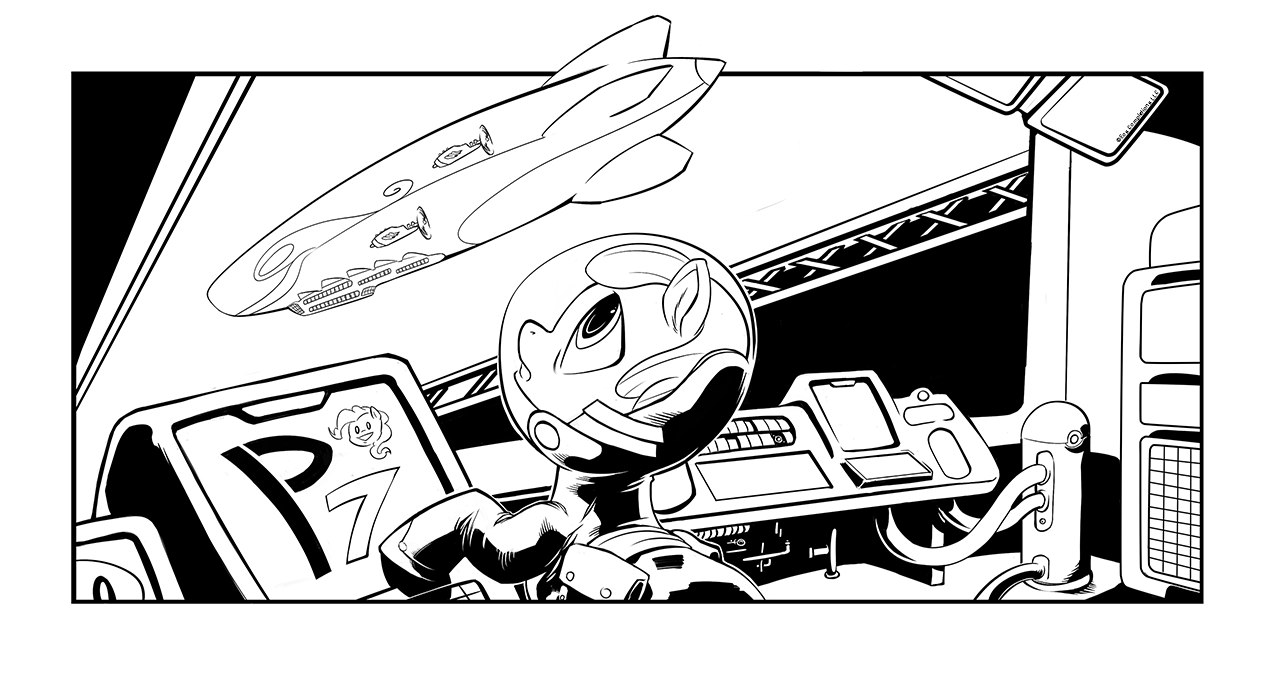
\includegraphics[width=\linewidth]{image04.png}

\begin{intro}
    Do you know you're all my very best friends?
\end{intro}

\englishdaytimeplace{4}{3:15 P.M.}{The Glow, Salt Cube City}

``That's impossible: ghouls are super stoopid zombies that eat ponies! You are ugly but mighty fine ponies, you can't be ghouls! If you're not telling me where the ghouls are I'm going to look for them on my own! BLEH!'' Puppysmiles stuck out her tongue.

Soft Air and Peach Blossom exchanged a rapid glance, then Peach spoke. ``We have no reason to lie to you, Puppy: we are ghouls, not every ghoul is a mindless pony eater.''

``But they told me-''


Puppy stepped back, afraid of the decomposing pony that was scolding her, or maybe scared by the truth in her words. ``B-b-but-''

Peach stomped a hoof on the ground. ``Stop playing the innocent foal! You're a monster like us! Stop pretending! Now!''

The little filly backpedaled, falling on her haunches and trying to hide her face with her hooves. ``Please! Please stop! I'll behave!''

``I don't want you to behave! I want you to WAKE UP!'' The ghoul mare stomped a hoof on the ground to empasise her last two words.

Soft Air put a hoof on Peach's shoulder. ``Please calm down, I don't think she's pretending; don't let your anger drive you.''

The ghoul mare shoved away Air's hoof. ``She's two hundred years old, how can she be this naive? Is she a retard? I think she's just playing with us, I think that we should''

Peach was interrupted by a long eerie wail. For a moment her mind rushed back to her foalhood, \emph{to that very day when she closed herself in the cellar by mistake and nopony came looking for her until night had fallen. She recalled the fear of being forgotten, the loneliness, every single creak from the barrels. Peach almost lost her voice calling for help but it was the fair day and nopony heard her}. With an overwhelming sense of guilt she realised that Puppy wasn't playing with them.

All the ghouls turned their attention to the filly in yellow; her long howl had something supernatural: it was the stuff of nightmares made audible and struck hard on everypony in the camp. Maybe this happened because they were used seeing a ghoul's rage but this was the first time in decades that they had heard a foal's cry. Even Sand Box hesitated for a moment before walking to Puppy and hugging her.

``What\dots what the hell is she doing? That sound\dots'' Peach staggered, trying to stand on her hooves.

``I think that you made her cry,'' Soft Air Answered flatly. ``Well, now I guess that it will be easier to make her accept the fact that we are the bad guys, right? Mission accomplished\dots''

``Oh for pete's sake, can you make her stop?'' Complained a pony with an orange helmet on his head. ``I can't hear my thoughts!''

Sand Box continued to hold the foal as her sobs gradualy lessened, growing quieter and quieter until they could barely hear her whispering half-spoken apologies. ``Now, now, I'm sure you are a good pony. You just miss your mom and this is ok,'' the ghoul leader rubbed Puppy's shoulders, ``everypony has a bad day here and there. Peach Blossom was quite upset but now you will say that you're sorry and she will forgive you; just please, pay attention to her when she is explaining something important, okay?''

Puppy nodded slowly and tried to establish eye contact with Sand Box, finding some relief in his elderly eyes. The foal turned to the ghoul mare and lowered her head. ``I\dots I'm sorry I didn't believe you, missus Peach Blossom\dots I know that you are a ghoul now, I was wrong.''


Did I already say that Puppy was easily distracted?

The filly in yellow scratched her helmet thinking about this brand new question, but she couldn't seem to find a proper answer. ``I think\dots this is because those pretty ponies promised me a piggy ride on a two headed cow if I came here, took a look around and go back and tell. They were also speaking of how great it would be if the ghouls were totally gone.'' Puppysmiles paused for a moment, trying to remember the rest of the story. ``Oh, right, so I said that I was going to deal with the meanie ghouls but they told no. I replied that I was big enough to shoo a ghoul away whatever it was and they made me promise to just come here and take a look\dots but I crossed my hooves so that promise doesn't count.'' The filly smiled widely, clearly proud of herself. ``I was smarter than them!''

Soft Air snickered. ``Oh sweet Celestia, this filly is hilarious. Can we keep her?''


\horizonline

\englishdaytimeplace{4}{4:00 P.M.}{The Glow, Salt Cube City}

Puppy loved her new Pinkie Pie plushie, hugging it tightly when she wasn't showing it to everypony she met. Too bad that it was mostly Soft Air. ``See? She is super cool, way better that that killing pinkbot! I bet she's super soft!'' The filly in yellow poked the plush with a hoof. ``Aw stoopid space suit! I want to kiss her but I can't! I'm calling her Silky Tail!''

Soft Air knocked on Puppy's helmet. ``Hey space pony, look at what I got here.'' The ghoul held out a holotape for Puppy to see, ``Guess what is this?''

Puppy tilted her head. ``Uh, a\dots black\dots thing? I know I know! It's some stuff that does other stuff!''

``Wow, I couldn't explain it better. Okay little miss scholar, come here and let me connect it to your suit.'' The ghoul Took Puppy's left hoof and opened a small socket on her wrist, then slotted the tape inside.

``{\mt Backup copy initiated. Reading. Warning. System working in emergency mode. Reproduction is impossible. Backup copy finished. The file will be opened as soon as the system will be running on normal mode.}''

``Hi mister Voice!'' Puppy waited for a moment but she got no answer. ``See what I mean? I don't even know what I did to him but he's keeping a grudge since we arrived here.''

``Oh, don't worry, it's just the salt cube. It interferes with smaller talismans and their circuitry.'' Soft Air watched the smiling foal for a moment: she was totally listening to everything and probably understanding nothing. The ghoul sighed. ``It makes mister Voice sleepy. He'll wake up when you two leave the Glow.''

Puppy nodded. ``Don't tell this to anypony but I feel a little lonely sometimes\dots I don't mean that I have no friends, but in the last few days I walked a lot and everypony had something else to do and nopony really wanted to stay with me, so\dots'' Puppy lowered her eyes. ``Mister Voice is a bit stoopid and he uses fancy words and he's grumpy, but he never leaves me\dots I hope he's not angry.''

Soft Air was going to say something but he was interrupted by the sound of two ponies arguing with each other.



``It will release in seven, eight hours at best as soon as we start moving it and if we wait it could be even too late to try anything.''

``Now I wonder why this came out all of a sudden. That damn cube was here even before the Dome was built and you give me a seven hours warning before apocalypse?''

Puppy turned her head toward the voices. ``What's going on?''

``I have no idea, little one.'' Soft Air frowned; this was bad news, but there was no point in explaining the situation to Puppy: bets were that she didn't even understand it and if she did, it could only make her panic. ``Hey, do you want to see the gift shop in the northern hall?''

\horizonline

\englishdaytimeplace{4}{4:45 P.M.}{The Glow, Salt Cube City}

``\dots And this is how Equestria was made,'' concluded Puppy.

``Ah, yeah, that was an amazing story but I asked you who is this Questioner you were talking about.''

``Oh, that story! Nay, it's boring. What about that time that I ate a butterfly?''

Soft Air lowered his head, sighed and muttered, ``I was running down the street when I saw a super duper mighty pretty\dots.''

At the same time Puppy started talking while jumping all around. ``I was running down the street when I saw a super duper mighty pretty\dots.''

\horizonline

\englishdaytimeplace{4}{5:15 P.M.}{The Glow, Salt Cube City}

Sand Box poked his head inside the gift shop, spotted Puppy and Soft Air and sighed in relief. ``Oh, here you are. You shouldn't wander this far from the Glow, there could be ferals in the area.''

Soft Air chuckled. ``Oh don't fret about that: little miss miracle here solved that problem.''

Sand Box tilted his head. ``You mean\dots she was attacked by feral ghouls?''

``Eyup: four at once, it seems; I'd say that this little filly can fend for herself.''

``I hope so,'' sighed Sand Box, ``because I desperately need her help.''

``Hi mister Ugly Pony Boss!'' Puppy jumped in front of the ghoul leader sporting a broad smile, ``I like this place! I had a great idea! I can say to the ponies of the other town that all the ghoulie are gone so they will never ever bother you! Then we find some nice dress and you'll disguise as\dots uhm\dots something not ugly and change your names, like in madame Le Flour and such! Isn't that a great idea? Oh, yeah, and we'll need a trombone!''

Sand Box cocked his head, then a sad smile spread across his decomposing face. ``Oh, I'd love to try that one, really, but I came here to inform you that we are going away: we leave the Glow.''


Sand Box sighed and put a hoof on Puppy's helmet. ``Don't fret your pretty head, my little pony: this is not your fault; it's just something that needs to be done, but I need your help.''

``Sand Box, could you please explain to me what's going on? I overheard you and Get Well talking about the FFO. Has this something to do with that cascade you were mumbling about when we arrived?''

Sand Box adjusted his glasses. ``Indeed. We already knew that the cube is not stable: during the years it absorbed and released the radiation from the megaspell following a cyclic pattern; As I already explained, during the last months this cycle accelerated. I think that the cube reached a point of non return and in less than five hours it's going to release.''

Soft Air's expression darkened. ``Well, this is not leaving exactly a lot of time. So, what now? I reckon that the Friend Force One still needs more than a little work. Are you sure about this release thing? What will be released, any idea?'' The ghoul already knew the answer, but he still had the hope of being wrong.

``I'm not sure about that. Could be the biggest mag pulse ever or the original balefire that was embedded into the zebra's warhead: when the missile hit the Dome the cube absorbed the matrix of the spell. The problem is that we are speaking of a huge chunk of pure salt that wasn't designed for some anti-megaspell defense; its behavior is highly unpredictable at best, a death sentence for Salt Cube City at worst.''

Puppy tried to follow the discussion but it was too technical for her: they used all sorts of fancy words mixed up with other terms that she wasn't even sure that were real words; so she decided to go and sightsee some other places of the Dome by herself.

Soft Air put a hoof on Puppy's helmet, pinning her on the place before she got away. ``Well then, but the FFO navigation system needs calibration and the autopilot is not working.''

``True. In fact I won't depend on those systems: I'm fly the airship myself.''

``Are you kidding me? It's suicide! Moreover, you can't fly that behemoth on your own, it requires at least somepony in the engine section and a lot of work around the hydrogen tanks.'' Soft Air looked for a moment at Puppy, then a shade of fear appeared on his face. ``Are\dots are you going to ask her to\dots''

``No, don't worry, she's just my ticket out of here: MK VI suits artificial intelligence talismans were a sub product of the P7 project. She'll be able to operate the control room just by stepping inside it and this will buy us time.'' Sand Box hesitated, ``Did you really think that I could take her with me?''

``Listen, we could simply evacuate the area and let the Cube blow those bastards in Apple Tower; we don't owe them anything, they even shoot us on sight if we try to leave the Dome. Let's hit the tunnels and let them taste this muffin.''

Sand Box looked straight into Soft Air's eyes. ``You can do whatever you want. I'm asking Puppy to open the roof and give me clearance for the take off. I don't know how far I'll get, but I refuse to be responsible for the death of another single foal. In those towers there aren't just the ponies you hate, Air: you are forgetting the foaling mares and the young ones: do they deserve your hate, too?''

Puppy was still trying to move, pushing with her helmeted head stubbornly but without avail against Soft's hoof. ``Lemme go! I wanna play outside!''

Soft Air looked at Puppy: so naive, she wasn't even aware of the horror she was already living. Even telling her to run as far as possible could have been useless; she was freedom itself and if a megaspell was really going to detonate\dots ``I can work the engines, just tell me what to do.''

Sand Box nodded. ``I knew I could count on you; Peach is coming too, and Dr. Get Well is already aboard working on the commands. The others are preparing the cube for transportation, now I need to teach Puppy her part, this may take a while.'' The ghoul leader looked at the filly in yellow, ``Hey, little one, want to explore a new place?''

\horizonline

\englishdaytimeplace{4}{6:30 P.M.}{The Glow, Salt Cube City}

\emph{``One more time, sunshine.''}

\emph{``But mommy, I repeated it one gazillion times!''}

\emph{``Just once, this is a super special secret magic spell. You have to say it without mistakes or it will not work. One more time for mommy, please?''}

\emph{``Uh, can I have muffins then?''}

\emph{``It's almost lunch time, but you can have muffins if you'll eat all the alfalfa.''}

\emph{``That's not fair! You always give me too much of it!''}

\emph{``And you'll get even a super double hug.''}

\emph{``Uh\dots okie dokie. When I'm in front of the large round door I have to put the hoof on the green button.''}

\emph{``Very well.''}

\emph{``Then the genie will ask me the Eye dentification cow. And I must say. Uh\dots a hint, mommy?''}

\emph{``Oh I know you remember it, just wait a moment and think again. Mommy knows that you are a smart pretty pony.''}

``{\mt Please state your identification code.}''

``Uh\dots FT\dots 0\dots 0\dots 1\dots 6\dots 5\dots RD\dots C\dots 1\dots G\dots A''

\emph{``Right! See? It's easy, I knew you can do it, and then what happens?''}

\emph{``Uh\dots the genie asks the other word\dots the pass code\dots''}

``{\mt Please, state your pass code for this ID.}''

\emph{``Yes, and you must say\dots''}

``Hi, I'm Puppysmiles!''

``{\mt ID accepted. First class field technician Rainy Days. Access to the control room granted. Warning. There are three thousands, six hundreds and ninety eight error messages to process.}''

\emph{``And remember, if you hear the loud honks you must run to the secret place I told you and use the magic words. Don't wait for me, understood?''}

\emph{``Sure mom!''}

\emph{``I love you Puppy, now come here and get your hug\dots''}


Behind the doors there was a large room with blinking panels. The far wall was actually a clear sheet of glass, covered in a spiderweb of cracks, and the whole room was illuminated by a couple of flickering lights in the ceiling. When Puppy stepped into the control room the door closed behind her.

``{\mt Warning. Mild radiation detected. Threat level: negligible. Activating all systems.}''

``Mister Voice you are back! It was about time\dots''

``{\mt All systems are working properly. Detected an attempt of opening a communication bridge. Checking source. Source confirmed: Ministry of Morale structure ID 00201 -- Salt Cube Dome Control Room. Comparing protocol. Warning. This suit system version is outdated. Updating, please wait.}''

``Wow, you sure chat a lot. Did you miss me? I missed you a lot! I found those ghoulie ponies we were looking for, but they were not evil! Instead they were nice, just a bit ugly\dots And Peach scolded me, but I was a bit meanie with them so I said I was sorry and then it was all right! Then mister Soft Air gave me a-''

A sudden ringing noise interrupted Puppy. She derped for a moment before launching herself in search of whatever made that funny noise. After some jumping and skipping, the filly found a red telephone just in front of a dusty desk. Puppy picked up the receiver, ``Hallo? Mom's not here and I'm too little so I can't take a note. Can you call at dinner, pretty please?'' The universe d'awed.

A familiar voice came from the phone: ``Puppy it's me, Sand Box. Good, you are in the control room; I reckon that my hacking tool worked. Here we need still some time to finish replenishing the battery boxes and pumping the hydrogen. It is very important that you stay in the room. ''

Puppy looked for a moment at the weird transmitter that Sand Box had given her before they parted. ``Oh right, the thingy! I didn't use that, I forgot!''

``But how did you\dots doesn't matter, now please listen carefully to me: I'm going to hang up the phone, but I'll call you back when we are ready. Wait there and don't touch anything until I call back, okay?''

``Okie dokie loki! Bye bye!'' Puppy put down the receiver and started looking around. The whole place was dusty and grey, quite a sad room that reminded Puppy of that stoopid place with the humongous round door; only this one was little and with a lot of desks and screens, mostly broken.

Suddenly a line of red lights appeared on the big desk in front of the damaged window; other red lights came to life on almost every desk and a couple of screens started flickering with a green light. Puppy sat on her rump, a bit disoriented. ``Hey I didn't touch anything! Cross my heart!''

``{\mt Update complete. P7 lite client version properly installed. Rebooting system.}'' The whole suit went dark and Puppy again felt that sensation of immobility just like the day she awoke in Canterlot, but this time it lasted for less than a couple seconds.

``Uh, I feel funny\dots''

In front of Puppy's face the HUD of the helmet flashed with a pink light that occupied her whole vision. In the middle of the pink square there were seven balloons tied together, then the logo disappeared leaving the usual interface with the compass on top and the other useless things down left and right. What really surprised Puppy was the voice: it wasn't mister Voice, but a different one; a feminine voice that was quite high pitched and very friendly.

``Hi there miss Days! We have a little bit of a situation here, all the screens are gone for good and we miss\dots uh\dots 100\% of the personnel. They haven't been to work for\dots woah, that's a lot of time! The bigwigs should seriously consider a little turnover here\dots Oh but don't worry! I can operate everything just fine from your personal console!''

"Who are you? Where's mister Voice?''

``I'm Pinkie Seven! Your best friendly pony-machine interface! I'm programmed to not try taking over the world nor become a judging god machine! I'm pretty nice, aren't I?''

Puppy scratched her helmet for a moment. ``Do you know miss pinkbot?''

``Why yes! Our top of the line entertaining prototype! It's being tested at\dots no wait, the test ended a couple days ago, let's see the results\dots well, it seems that the party was so great that it made you simply die! No wait, it's intended literally\dots doesn't sound that good\dots well, let's never speak again of the pinkbot project, okie dokie?''

``But it hurt a lot of pretty ponies\dots''

``Data deleted. I'm sorry I don't know what you are talking about. Now, what was the other thing?''

``Uh\dots the pinkbot?'' tried Puppy.

``Never heard of it. Something else?''

``Ah\dots yeah, something about a\dots flying\dots something\dots'' Puppy tapped her helmet trying to remember. ``Where is mister Voice? I think I like him better.''

``You\dots you don't like me? You don't want to be my friend? But why, I'm trying so hard! I waited here for, like, two hundred years! Please don't send me back to the mainframe! It's dark and lonely and I can count only the machine cycles down there! PLEEEEASE!''

``Uh\dots if you're sure you're not going to foalnap somepony\dots''

``No way, there must be a rule against that in my program, don't worry. No foalnapping, no mass extermination, no moral judgment. Just your average little helping pony routine, don't worry! And\dots say, I know this is not going to help our relationship, but the security protocol is annoying me with a little detail.''

Puppy giggled. ``Tee-hee, miss Voice uses fancy words!''

``Yes, sometimes I do that\dots say, are you first class field technician Rainy Days? Because your console here says that your name is Puppysmiles.''

``Silly Voice! I'm Puppysmiles!''

``Oh\dots great, just what I needed: a breach. Two centuries in a dusty talisman and the first time I can have some fun it's an intruder.'' The voice paused for a moment, ``Miss Puppysmiles, your presence is not authorized. I must ask you to leave and you have no idea of how much this hurts me.''

``B-but\dots mister Sand Box said that I must be here or the Friend ship will not fly! Can I stay just a little more? Pretty please? Puppy please?''

``If you want to stay you need an authorization from the chief of the staff or from a military with at least the grade of colonel. I really really REALLY want you to stay but my hooves are tied! If I only had something to work with, I don't know, a logical paradox or some funny program loop\dots Oh, wait. What's your relation with the head technician?''

``Who?''

``Rainy Days.''

``Oh, she's my mom! Do you know where she is?''

``Oh but this fixes everything! Let's see, yes, I can move this here and that there and\dots voila! Today it's the bring your daughter at work day! Are you happy?''

``Uh\dots I still want my mom.''

``Hey, look at this, it's even in your mission logbook! You are really fond of your mom aren't you?''

``Well, duh, she's my mom!'' Puppysmiles deadpanned.

``Listen here! We can make a- oh wait, call incoming on the emergency line.''

The voice of Sand Box replaced the one of the artificial intelligence. ``Hey Puppy we have done here, are you ready?''

``Hi mister Boss! Sure I am, this miss Voice chats a lot!''

``Great, now listen carefully: there are a couple of ponies that want to say goodbye. Please behave and do not take too much time because we are running a bit late.''

The voice of Sand Box was replaced by Peach Blossom. ``Hey, little one\dots are you there?''

``Hi miss peach!''

``Good, I'm so happy to hear you. I wanted to say that I'm sorry, I didn't have to scold you. Peace?''

``Uh\dots. okie dokie?''

The ghoul mare sighed in relief. ``Thank Celestia, I couldn't do this with that weight on me. Please remember this, Puppy: Equestria is an unforgiving place, you have to treasure your friends because they will be very few. I\dots I regret that we didn't have time to know better each other, but I know that you are going to be safe, so I have no regrets.''

``Are you going away? I can come and visit you when you arrive, okay? We will trow a party!''

Peach took some moment before talking again. ``Yes\dots yes Puppy, if we will meet again one day, we will `trow' a super party\dots sorry I have to go.''

The phone went mute for some moment before another voice started talking. ``Hey Puppy, Soft Air here. Please follow Sand's instructions very well, we're all counting on you here!''

``Hi Soft! Mister Voice now is miss Voice! Isn't that funny?''

``What are you talking about? Aw, doesn't matter, I have to tell you something: I knew your mother. Now please don't panic, I have little time and you really need to listen.''

``You\dots why didn't you tell me that earlier!?''

``I\dots I wanted to do that but all this megaspell thing dropped on me before I could. I'm telling you now, so please listen: I was under her command, third class technician Soft Air of the Third Armored Company Steel Flanks. Do you remember that tape I gave to you?''

``Uh\dots the black stuff that does other stuff?'' Puppy tried hard to remember.

``Yes, that one: it is the location of our field headquarters; it's located south of Salt Cube City, in the marshes. If you can find any clue about the chief it will be there. So, when you have finished in the control room just set the 165Th Brigade field Headquarters as primary objective and follow the pink arrow on the compass. Did you understand everything?''

``I\dots yes, sure: go head quartet, find mom! Thank you mister Soft Air you are the best pony!''

``I think you misspelled Pinkie Pie,'' P7 chimed in.

``Oh, and one last thing, Puppy: in your journey you are going to learn things that will hurt you. It's unavoidable, but I know that you are a brave pony so\dots please, don't forget these days and the days before the megaspells. Equestria now is a scorched dying land, but you know that it wasn't always like this. Don't let the wastelands scorch you heart, too; watching you I still can see the sun shining in the sky.''

``Uh\dots why is everypony saying sad things? You are only going for a little fly, it's not that we will never meet again; me and mommy are totally coming for a visit when you will find a new home.''

``I\dots You are incredible, Puppy. You make me miss my sister so much\dots Be safe and never forget to smile. Soft Air, closing.''

``Puppy, Sand Box here. Are you listening to me?'' The elder ghoul's voice interrupted the conversation.

``Ah\dots yes Boss\dots say, we are going meet again, right?''

The was a long pause, then the voice of the ghoul arrived calm and somehow very sad. ``I'm sure that in the end we will meet again and we will be together, if you want this to happen. Never lose hope, Puppy.'' There was another pause before the Ghoul Leader started talking again: ``We need you to open the roof and give the green for the take off. Now, repeat what I say: activate Voice Console, Authorization code SB01, chief researcher. Pass code Agatha. Override priority list from one to eleven\dots''

\horizonline

\englishdaytimeplace{4}{7:30 P.M.}{Downtown, Salt Cube City}

Sage Brush was sitting at his window with his sniper rifle ready, guarding both the Big 52 heading south and the Dome outskirts. It had been a long shift but now the daylight was beginning to fade and within a hour the earth pony was going to put his cutie mark under a table. Hopefully with a good bowl of onion soup in front of him.

``I wonder why they sent that filly in the Dome all by herself\dots she's been inside since lunchtime. Poor soul, now we're even sending kids to their deaths\dots'' The pony spat down the window and activated the night vision of his rifle sights.

And in that very moment what was left of the eastern section of the Dome's roof began to collapse with the deafening sound of screeching metal.

``Luna rape my soul, what is going on there?'' The guard looked down the scope to try and see what was happening.

After several minutes of observation, Sage was sure that the roof was not exactly collapsing, not completely at least: there were parts that simply fell down and there was a large amount of dust being thrown up, but he could clearly make out that the entire structure of the east wing was\dots rotating? The two hundred years old cover of the Dome was almost fused into a single block by rust, but now an incredible strength was simply tearing apart every metal plate that didn't want to move; that giant fossil from the bomb days was sliding on completely forgotten metal rails that in more often than not couldn't sustain the stress and cracked.

None the less, the roof was still moving. Slowly, and causing itself an irreparable amount of damage, but it moved. Now that the largest part of the debris was gone, Sage could see that there were two separate sections, similar to the doors of a cellar; the `doors' were sliding in opposite directions, creating a rectangular opening that was as large as a town square.

The noise created quite a commotion in Downtown: everypony ran out of the tents to see what was going on and some mares simply fainted, screaming things like ``The horror the horror!'' and such. Sage was made of sterner stuff and kept his head calm while aiming his rifle towards the hole.

``Ok zombies, let's see what's going on in your rotten heads.''

A section of the roof stopped moving with the sudden sound of twisting metal and snapping cables. After less than a minute, the other half of the gigantic hatch finished opening, then the sky went pink as a thousand spotlights dotted the clouds. There was an explosion of blue and green smoke with a shower of confetti all around the Dome and then a high pitched voice started talking.

``Fillies and gentlecolts!'' The voice came from the speakers of the dome: it sounded crackly and fuzzy but where one loudspeaker failed another fifty kept the pace. ``Glory to our beloved and magnificent princesses Luna and Celestia! It's with immense honor that today I'm here to assist the launch of the newest and most incredible technological jump in the field of mass transportation! Thanks to the \emph{Friend Force One} and her many sisters that will follow, Equestria will never seem so small to you!''

Boisterous music played loudly for a few seconds.

``And now let me introduce our guest of honor! The daughter of first class technician Rainy Days, Puppysmiles!''

``-and then I said: Oatmeal, are you CRAZY?'' There was a long pause. ``Uh, was that my voice?\dots LALALALALALA! Hey, it's fun! Goodbye ghoulie ponies have a nice trip! Send me a postcard!''

Sage brush raised both eyebrows. ``What the hay is going on? First what Rainy who? Who's this Rainy Days? And what\dots is\dots that\dots thing?

From the opening in the Dome, an odd shape slowly emerged: it was like a balloon, but it was very elongated, like a gigantic corncob pointy at the ends and larger in the middle; the flying machine had four fins at the back and it was completely pink, save for a white oval on each side in which was written 'Friendship is Magic!'.

Sage rubbed his eyes and tried to pick his jaw back up off the floor. Now the airship was rising above the dome and slowly rotated itself; under the humongous pink balloon there was a structure similar to an air wagon but way larger. On what the guard pony decided was the rear side of the cabin, there were a couple of large propellers and other two were placed immediately under the two horizontal fins next to the tail of the balloon.

The thing began to gain speed, it avoided the Towers and headed south-east. Sage still looked in disbelief at the balloon flying away when the high pitched voice from the Dome spoke again. ``Very well everypony, I guess that's all, remember to buy war bonds! This Show was brought to you by the Ministry of Morale, and remember, Pinkie Pie is not happy if you are not happy! So smile, because she's watching you FOREVER!''

The Balloon was already half a kilometer away when the lights from the Dome finally shut down and the music stopped. The roof tried uselessly to close again but this simply led to a new concert of bending metal, snapping cables and falling debris.

``Holy mare\dots she\dots they\dots they are gone\dots the ghouls simply jumped on that\dots thing and\dots they flew away?'' The guard scratched his head, ``Why didn't they do that before!? Where did they get that ridiculous air thing? Friendship is Magic? This place is going crazy.''

Almost half an hour later the ponies had already gone back to bed and the Airship was just a point in the distance, ten kilometers away; it wasn't moving very fast if compared with an air wagon, but it was way bigger. The sound of hoofsteps from the stairs should have alerted Sage Brush, but he was still looking at the balloon flying away.

A mare with a combat saddle knocked on the wall before entering the room where Sage was stationed. ``Shift time. Hi mate, was it exciting?''

The guard turned to face his comrade. ``They\dots just flew away! In a gigantic balloon! I\dots I don't get it, why did they fly away!?''

The mare tilted the head while looking outside. ``Hey, now that the light is gone don't you feel that something is missing?''

``Yeah, the ghouls and another third of the roof from the Dome.''

``No, that's not what I mean. Look better. Where is the glowing light?''

``Oh buck me, you are right! The Dome is not glowing! It's\dots dark and\dots ghostly\dots and scary\dots''

``So\dots they went away for real\dots tomorrow morning with some light we have got to go there and check the radiation.''

``Do you think that-'' Suddenly the world became blindingly white. It was so strong that even with his eyes closed Sage could see it. He waited for the light to go away for what it seemed an eternity until\dots

SKRA-KRACK!

It was the loudest sound ever: something halfway between the sound of a thunder and the whistle of a tornado, only louder. Driven by his instinct, the guard grabbed his friend and tried to gain shelter behind a wall.

Immediately after the sound came the rumble. At first it was nearly impossible to percieve, but in a matter of seconds it became an earthquake and with it arrived a solid wall of dust that hit Downtown, flattening most of the tents in the market but barely scratching the heavier structures.

``Wh-what was that?'' Sage rubbed his eyes, trying to open them.

``I don't know\dots the ghoul's flying machine exploded? It seemed something like a gigantic spell going\dots'' The mare realized what this implied. ``Oh fuck. A megaspell. They had a damn megaspell on that flying thing!''

~\vfill

\begin{engnote}
    Level up! (3)
    
    New perk added: Intense training - Charisma ($7 \to 8$) now you are 14.28\% cooler
\end{engnote}






\chapter{Chickens}

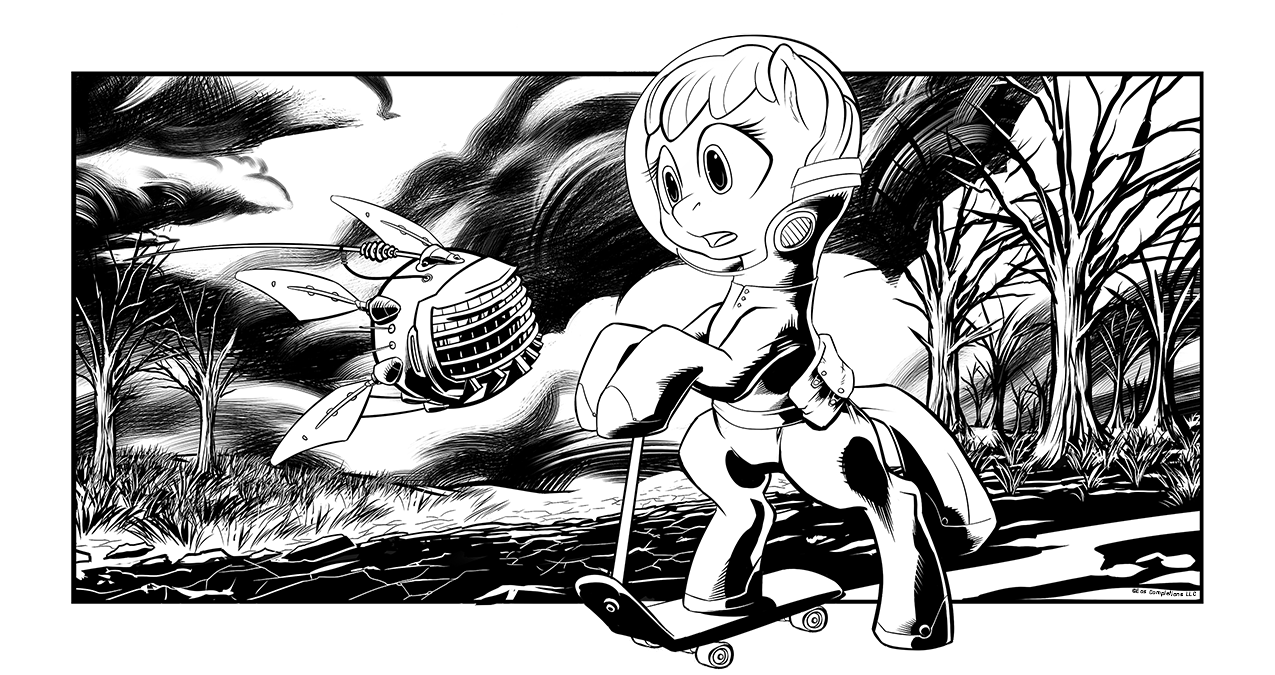
\includegraphics[width=0.9\linewidth]{image05.png}

\begin{intro}
Cutie Mark Crusaders Chicken Rescuers are go!
\end{intro}


\englishdaytimeplace{5}{9:30 A.M.}{Downtown, Salt Cube City}

``Yay! Go faster pretty cow! I wanna go faster!'' The left head of the brahmin sighed and threw a desperate look toward the nearby unicorn with the black hat.

The pony snickered at the cow and waved a hoof, dismissing her mute complaint. ``It's the deal, no grudges. Give the foal one last ride then bring her to my office.''

``All right, Mister White.'' The cow sullenly began to trot around the outside of White Tower, a journey she had made several times in the past half hour. The ponies in the streets were busy repairing the damages from last night's shockwave, but Puppysmiles still drew a lot of attention from them. And with the glares also came low, muttered words.

``I know her, she's that ghost from the Carnival. She cursed the ghouls. That foal brings bad luck.''

``Look, she's making a fool out of the White Apples. I bet all my caps that she's blackmailing them with things that she discovered inside the Dome.''

``Have you seen? The Glow disappeared and then---then the ghoul's airship exploded. They tried stealing something but it backfired. Filthy ghouls, they deserved that one.''

``Yes, but what is she?''

``Don't ask, I've never seen her eat or even open the helmet. I don't know what that means, but I'm sure that she's up to nothing good.''

``Shush! She's coming this way!''

Puppysmiles was having a good time and didn't care about the strange glances. It was unlikely that she even noticed them. ``That was super fun Missus Cow. Can we do it again sometime?''

One of the two cow heads nodded. ``Sure, but you have to ask Mr.~White. He's waiting for you in the office. Just go inside and take the red door,'' the other head continued to ruminate.

Mr.~White's office was a large, clean affair, sporting a variety of pictures decorating the walls as well as a mahogany desk so highly polished that you could see your reflection in it. ``Woah, this place is super duper fine, Mister White!''

The chief of the White Apples was a male unicorn that wore a black hat on his head. His coat was white, and his mane cyan. ``Well, thank you, Miss Days.'' This name won a puzzled look from Puppy, so Mr.~White elaborated. ``The voice from the Dome last night said that your mom was named Rainy Days, so I imagine that your full name is Puppysmiles Days, isn't it?''

Puppy slowly nodded and tilted her head. ``Uh, yes it is. Now I have to go. Miss Voice put a new arrow on the compass so I have to follow it. Can I go please?''

White sighed and lowered his hat in front of his eyes. ``Sure, but I'd like to ask you one last thing. What was that glow inside the Dome?''

``Ah, you mean the Salt Cube?'' Puppy giggled as if she found that question funny. ``You silly pony, haven't you ever seen the Salt Cube of Salt Cube City? I mean, you live here, \stpr{duh!''}

White felt the urge to raise his voice, but the filly had a very simple mind and scolding her was useless at the moment. Instead he smiled. ``I must admit that I've never been inside the Dome. It is a bit scary, if you wish. So, the ghouls took away the salt cube on their vessel?'' Another puzzled look came from Puppy. ``The flying balloon?''

She nodded. ``Eeyup! They took the cube and they did that quite in a hurry, too! They were all talking about a cascade and something about a dee---uh, de-tuna show.'' Puppy didn't seem very happy with that last term. ``Something like that, I can't remember. But they were saying that they had to go away before it happened because it was dangerous.''

``Detonation, maybe?''

``Yes! They said detorn\dots uh, deetun\dots that one. Anyhow, it was inside the cube and they wanted to go away with it super fast. I helped them!''

He raised an eyebrow. ``They wanted to go away as fast as possible with a time bomb? I knew that those ghouls were crazy, but I didn't think that they were gone this far. Oh well, I guess that this explains why the radioactivity around the Dome is fading.'' Mister White smiled thoughtfully. ``You did a good job, little one. I'd like you to stay a little more, but if you want to go so badly, I guess that I'll let you follow your road.''

``Okie dokie, Mister White! Bye bye! I'll tell my mom that you were super nice to me!''

``Sure, have a nice trip, little one. Sorry if I'm still a bit curious, but where will you go?''

Puppy pointed a hoof southward. ``There! My mom is just at the other end of the arrow!''

``Oh, straight into the marshes. Good luck and take care!''

She was so dead.

The marshes were the worst area in the northern branch of the Big 52, and a foal alone was just going to be some radigator's breakfast. It was a pity to waste that radsuit, but the White Apples were not raiders.

Mister White stopped for a moment, pondering that last thought. She was already going away, but something in that little pony made him regret having used her so badly. She probably saved the tribe from a fate way worse than the ghouls, and he had given her, what? Just a cow ride and not even a forewarning of the incoming danger? Not fair. ``Hey, Miss Days, wait a moment! I have something for you.''


\horizonline

\englishdaytimeplace{5}{11:30 A.M.}{Salt Cube City Outskirts, Big 52 N Branch}

``WEEEEEEEEEEE!'' A yellow bolt dashed along the road riding a red scooter.

The last houses of Salt Cube city's suburbs zipped past Puppysmiles, leaving a landscape of abandoned corn fields in their stead.

\stpr{And please, keep this in mind. Once you reach Happy Straw you have to take the detour. The route through the swamps is---}BLAH BLAH BLAH! Blah\stpr{---and remember! Don't try in any case to cross the} blah blah boo-ring!

The filly-propelled vehicle zoomed directly south and, since the scooter wasn't loud enough by itself, Puppy was providing the sounds. ``WOOOOSH! ZOOM! Straight to the moon! Space Captain Andromeda to the rescue! YAY!''

Ahead of her, the road ran through rotten fields and ruined farms, straight as a sunbeam heading toward her objective. After a hoof-full of kilometers, the fields became a barren land dotted with dead trees and small pools filled with murky water. Here and there rose a shack or a small camp, but they all seemed old and abandoned. There was some life in the area, but it consisted mostly of insects and other nasty creatures that instinctively left Puppy alone.

What was not seemingly eager to ignore Puppysmiles was the spritebot that stood right in the middle of the road about a hundred meters in front of her.

``BEEP BEEP, I'm a jeep! Space pony incoming!'' The spritebot seemed to ignore this information, but Puppy wasn't the kind of foal that stopped for anypony while she was having fun. The yellow bolt simply kept going at top speed on her brand new scooter. The spritebot dodged at the very last moment and seconds later was following on Puppy's heels, trying to keep up with her pace.

``Hi, Puppy, are you in a hurry?'' A familiar voice came from the spritebot's speakers.

``Questioner! I was missing you! Have you seen my new scooter?'' Puppy giggled, still cruising at top speed. ``I knew another talking robot, but this one was funny! Well, it wasn't exactly a robot. I'm not sure.''

``How wonderful. Care if I ask you something?'' He didn't wait for a reply. ``What happened in the Dome, and what was that explosion east of Salt Cube City? Hey, could you stop a moment, please?''

Puppy sighed and slowed down. ``Gee, I was having fun.''

After stopping and jumping from her brand new ride, the foal tapped the bottom of her helmet as if it was her chin as she thought about Watcher's question. ``What happened in the Dome? I made a lot of friends---Mister Boss Sand Box, Mister Soft Air, Miss Peach Blossom\dots Oh, and Miss Voice.''

``Wasn't it Mister Voice?'' Watcher tried to correct.

``No, silly robot, there is a Mister Voice AND a Miss Voice! She had to stay at the Dome, but Mister Voice can call her whenever I need! She is super cool and helped me with the goodbye party for the ghoulie ponies!''

``Oh, another pony-machine interface routine. So, you met these ghouls and then threw them a goodbye party? What do you mean by that? Did you help them launch the airship?''

``Yush!'' Puppy nodded enthusiastically. ``It was super great! I was looking from the window and there was this \stpr{huge} thing that went up, up, up in the sky!'' Puppy spread her front legs to show how large the ship was, and reared up on her hind legs to show how high it was, but she went too far and fell on her haunches giggling. ``And there were all those lights and I heard my voice super loud, so I said `la la la' and `goodbye ghoulie ponies' and then they went away! It was scootastic!''

``Scootawhat?''

``Scootastic!''

``Is that even a word?

``Scootasure!''

``You know, I don't think that this scooter is good for your pretty head.'' Watcher's voice betrayed the slightest trace of concern. ``Back on topic, what about the explosion?''

``What explosion?'' Puppy tilted her head, frowning a bit. ``You mean the roof that went down?''

``No I---wait a second, another roof fell on your head?'' This piece of information took Watcher by surprise.

``Yup. After the roof opened and the big balloon went away the place went all squeaky and bang! Right on my head.'' Puppy giggled. ``But I'm a super space pony so I dug my way out! I'm just that good.'' She smiled proudly.

There was a short laugh, then a sigh from the robot speaker. ``Oh well, everyone has their talents. So, where are you going now?''

``To the next Mom's place, obviously. Third time's the charm!''

\stpr{BLAM! BLAM!}

A sudden pair of gunshots echoed through the air. The bullets didn't hit anywhere near Puppy or Watcher, but the filly heard them loud and clear. ``Hey, what was that?''

``I---Sorry Puppy, I have to go. There must be raiders somewhere. You'd better hide and wait until this firefight ends.''

``A firefly? Where? I love fireflies!'' Puppy immediately launched herself in a frantic search, jumping all around.

``Please, Celestia, keep her safe.'' The voice from the spritebot was replaced by fizzling music, and the drone simply began to drift away.

The sound of the gunshots came from above Puppy's head, and when she looked up she saw an incredible scene. Some big, flying ponies were dancing all around and making fireworks, like a majestic ballet. The sight took Puppy back to the day that Mommy took her to the flying grounds, and there were all the pretty pegasi flying and making super fun things in the air.

This time it was more or less the same. Well, actually not the same, but there was somepony flying, and there were lights and loud noises, so Puppy immediately classified the whole thing as top-tier entertainment.

But all the figures were pretty big, and didn't seem like pegasi at all. The foal frowned and asked, ``Hey, Mister Voice, what's wrong with those ponies?''

{\mt ``Analyzing. Friendly griffons.''}

Puppy hadn't the slightest idea of what a griffon was, but if Mister Voice told her that they were friendly, then it was A-OK. She waved a hoof and tried to get their attention. ``Hey pretty ponies! I'm here! Hey!''

One of the creatures turned to look down at the road, lowering his guard for a moment. He was shot by another of the creatures and went down spinning.

``Uh, Let's see, one, two, three\dots'' Puppy tried to count the remaining griffons, but they were a bit too fast for her tastes, so she decided to trot up to where their friend had landed. Drawing next to the creature, the foal noticed that it wasn't a pony at all. It looked like some strange beast, being half-eagle and half-lion, She decided that it had a funny look.

``Hi, Mister Chicken!''

The creature didn't move. A large pool of blood was forming under his body. Puppy poked him with a hoof. ``Hey, what's wrong?'' There was no reaction. ``Uh, Mister Chicken? Wake up? Rise and shine?'' Still nothing. This couldn't be good, but the worst part was that his friends didn't seem to notice it. Something had to be done.

``HEY! CHICKENS! YOUR FRIEND HERE IS HURT! COME DOWN!'' Puppy cried with all her breath and waved both hooves in the air, trying to get some help. Quite obviously, she was ignored. The remaining three griffons continued to dance their waltz of bullets and blood in the sky above her head.

``Aww, they're too busy having fun and they don't hear me!'' Puppy sighed. ``If only I had something to catch their---Wait a moment, I have it!'' She smiled, recalling that shiny thing that Mister White gave her. What-was-its-name? Nine miles meters? Nay meme liters? ``Uh, Mister Voice, gimme that shiny thing that makes a lot of noise.''

{\mt ``Warning. Object Puppysmiles cannot be retrieved from inventory.''}

``Hey! You're not very nice! You know what I mean! That thing, the nanny my litters! You know, that one from Mister White!''

{\mt ``Affirmative. Retrieving 9mm semiautomatic pistol.''}

The gun floated in front of Puppy.

She grabbed the iron with her hooves and pointed it at the sky. ``Hey! HEEEEY! Listen to me! How does this thing work? How does it do the noisy stuff?''

{\mt ``Loading instructions for shooting mode 'Time Crisis'. First: point your gun at the target. Second: pronounce the word 'fire!' or 'bang!' and the gun will shoot. If you need reloading, put your weapon in the inventory and extract it again.''}

``Uh, sounds easy!'' Puppy pointed at a griffon. ``Bang!'' \stpr{BLAM!} \stpr{Clank!} ``EEEP!'' Recoil sent the gun flying out of Puppy's hooves. It bounced against her helmet, falling to the ground a couple of meters in front of her and knocking Puppy down on her rump.

One of the griffons screamed in pain. ``Fuck, he has backup! Kill that snip---'' the creature didn't get to finish the sentence, as his head exploded in a cloud of blood. Now there were only two griffons dueling in the sky, but the battle itself was becoming a lot more personal.

The two griffons engaged each other in melee, biting and slashing with their talons. Puppy trotted over to the new fallen griffon and noticed that his head was missing. ``You know, Mister Voice, I don't think they're playing. Is this chicken, uh, dead?''

{\mt ``Affirmative.''}

``And, uh.'' Puppy frowned. ``The other chicken there?'' Puppy pointed at the other grounded beast. ``Is he dead too?''

{\mt ``Analyzing. No vital signs detected. The subject is dead.''}

Puppy's eyes rose again to the sky, where the last two griffons were fighting. ``And those two are trying to hurt each other?''

{\mt ``Affirmative. Every clue leads to the conclusion that they are fighting each other to the death.''}

``Okie dokie.'' Puppy paused for a moment, pondering the situation. ``How do we make them stop? Oh! I have an idea!'' Puppy took a deep breath. ``PLEASE STOP FIGHTING! SOMEPONY COULD GET HURT!''

Actually, somepony already got hurt. Well, mostly some griffon, but Puppy wasn't fussed about details, and the two surviving fighters didn't seem to pay attention to Puppy anyway. From her point of view it was quite hard to say what was going on exactly, but one of the two let out a high pitched scream and then they both began to fall in a rapid spin, like a whirlybird seed.

Puppy jumped on her scooter and launched herself on the chase, trying to see where they fell. When she reached them, she found quite a scene: one of the two griffons lay on the ground, his chest torn open on the left side and his throat cut; the other creature was struggling to get to his feet, but was losing too much blood from a multitude of wounds.

``Hey, Mister Chicken, are you all right?'' She rushed to the struggling griffon as he fell on the ground coughing. ``You don't seem all right.''

``\stpr{Cough}\dots You\dots are the foal that shot\dots Thank you\dots''

Puppy frowned. ``I what?''

``Please---\stpr{cough}---listen carefully. There is\dots my daughter\dots in the military---\stpr{cough cough}---south.'' The griffon's breaths were deep and labored, bringing with them a gurgling sound and causing him to cough again. ``Henrietta\dots She\dots is waiting for me there---\stpr{cough}---I beg you\dots go there\dots give her\dots this\dots'' The griffon handed Puppy another gun. This one was heavier than the one she owned, and it was black with a red line along the barrel.

``Uh, okie dokie?'' Puppy poked the griffon. ``Sure, but\dots you're going to get better, aren't you?''

``You\dots are you stupid or what\dots? I'm\dots dying\dots'' Another burst of coughs and blood interrupted the creature. ``Tell\dots tell Henrietta\dots that I wanted to go south with her\dots tell\dots her that I---\stpr{cough}---I\dots tell\dots'' His voice faded, and with it even the spark in the griffon's eyes disappeared.

Puppy waited for a moment, then tried poking the griffon with a hoof. ``Hey, Mister Chicken, are you sleeping? Mister Chicken?'' She poked him again. ``Uh, I think that I have to go. I, uh, am sorry.'' Puppy took a step back from the dead creature. She felt bad. Something was really wrong now. This wasn't the first time she was in front of a dead creature, not even a dying one, but\dots but she never really stopped to contemplate it before.

Now, if we were talking about your average pony, this would be a perfect moment to make her face the horrors of a world where brothers kill each other in a constant struggle for survival. Too bad that this is a story about Puppysmiles.

``Uh, I hope you get well soon, but now I really, really have to go. Sorry.'' The foal kissed the griffon goodbye through her helmet and jumped on her scooter, dashing away.

``Hey Mister Voice, are you there?''

{\mt ``Affirmative. All systems operational.''}

``Why do pretty ponies hurt each other?'' She frowned.

{\mt ``Warning. This routine is not meant for socializing.''}

Puppy sighed and kept scooting toward the pink arrow on her compass. ``Uh, Mister Voice? Did that chicken say something about a daughter?''

{\mt ``Affirmative. It is set as objective for secondary mission: Bad News, New Buddies.''}

Puppy pondered for a moment, stopping the scooter. ``Can you show me where she is?''

{\mt ``Affirmative: Henrietta Firebright set as new primary target.''}

Puppy looked at the pink arrow disappearing from the compass and reappearing again in the same point. ``Uh, I don't think it worked.''

{\mt ``Affirmative. New mission objective correctly set.''}

Puppy shrugged. Operating all the mumbo jumbos in the space suit was Mister Voice's job; if he said that it was okay, then it had to be so. ``Let's roll.''


\horizonline

\englishdaytimeplace{5}{14:00 P.M.}{165Th Brigade field Headquarters, Salt Marshes}

{\mt ``Warning. Several breaches in the containment. Warning. Compass offline. Warning. Radio offline. Warning. Medical system offline. Warning. Breach in the helmet. Warning. Pink agent detected. Repair talisman activated.''}

``Ugh, I think that I stepped on something.'' Puppy tried to get on her hooves, but stumbled and fell again. ``I feel dizzy.''

A couple of road signs right in front of her stated, ``Attention: minefield!'' and ``Military zone: access restricted.'' Debris and broken pieces of asphalt lay strewn across the road around her, and entire chunks were missing from the route ahead. Quite incredibly, the scooter lay a couple meters away from Puppy, showing almost no sign of damage.

``Hey, Mister Voice? Why did the road went boom?'' Thick pink smoke poured from the holes in the suit and the cracks in her helmet.

{\mt ``Analyzing. The cause of the explosion is a land mine. Radio is online. Helmet integrity restored.''}

Puppy frowned for a moment. ``What's a land mine? No, wait! This is going to take forever, right? With you using fancy words and me trying to not get angry and we start arguing again. I need a professional here! Call Miss Voice.''

{\mt ``Opening communication bridge. Please wait. Compass online. Medical system restored. Loading personal data for subject 001: Puppysmiles. Subject deceased, condition stable. All clear.''}

In less than five minutes the suit was almost repaired, mostly taking materials from the various pieces of junk that Puppy kept in her pockets. The foal wasn't very selective with the stuff she decided to keep. If it was shiny and colored, it was a go. The suit's repair spell  wasn't picky either. Anything that contained glass, metal or plastic was good enough.

``Hello hello? This is Salt Cube Dome emergency line. Sorry, but at the moment all the personnel are dead, so please call again when the services have been restored. Bye bye!''

``Hold on, Miss Voice! It's me, Puppy!''

``Oh, Puppy! Hi there, it's been a while! What's going on? Did you find that thing I asked you to find? I'm ready for activating transfer protocol as soon as you are!''

``Uh, nope, sorry, Miss Voice. Actually, I need help.''

``Oh don't worry, I've been waiting here for, what? Two hundred years? I can wait another couple centuries! So, what do you need?''

``Well, I was dashing like a Wonderbolt on my new scooter when suddenly---''

``Wait wait wait! You have a new scooter? Is it red?''

``You can bet your saddle!''

``Scootastic! Is it fast, super fast, or double super duper fast?''

``It's like the one you see on the signs with Scootaloo on top and all the stars around! You have to try it. It's totally crazy!''

``Aw, now I feel green! You have to find me that prototype body so I can try it! Promise me!''

``Sure! Pinkie Pie swear!'' Puppy tried to poke her eye, but the helmet was a problem.

``YAY! Okay okay, back on topic. You just wanted to tell me about the scooter?''

``Uh, no. Actually, I have a problem of exploding roads. You see, Mister Voice says that there is some mining, but I can't see the miners, and I don't think that mines go boom.''

``Well, it depends on what you are mining but I can see your point. So the road exploded and there are no miners there\dots I need you to take a look around, please. Do you see anything like a, ah, flat and large frying pan with an orange light on top? It should be ugly green or sadness gray.''

Puppy smiled. ``Yay, I see it! No wait, there's moar! It's full of them! There are orange lights everywhere! It's like fireflies! Wow!''

``Oh, so we are speaking of those kinds of mines. Okie dokie, I need to see them myself. Wait a second.'' The HUD in the helmet flickered for a moment, then the whole helmet lit with targeting signals, one for each mine that the suit's sensors located. ``Wow, forty-five and still counting! This reminds me of a game I used to play a lot!'' P7's voice paused while the sensor finished detecting all the mines. ``Done! Now, there's a path. You just do as I say, and we'll be on the other side lickety split.''


\horizonline

\englishdaytimeplace{5}{14:45 P.M.}{165Th Brigade field Headquarters, Salt Marshes}

The base was mostly intact. A line of big hangars stood in front of a large court with low armored buildings on the sides. The front gate had a couple of automated guns, but a large battle tank had crashed into it, nearly destroying the entire structure and effectively blocking the entrance for anything bigger than a pony.

Puppy stopped for a moment to rummage inside the tank before entering the base. ``Woah! This thing is full of shiny stuff! Look at this one!'' She took a large shell with a red band around the head. It was big, probably used as ammunition for the tank's main gun. ``It's pretty! Hey, there's more! This one is black and this one is blue! Tee-hee!''

After gutting the tank's ammo rack, Puppy finally decided to venture inside the base. There were more tanks that were positioned in the middle of the court, simply abandoned in place and mostly devoured by the rust and the climate of the swamp. Strange plants grew all over the place and out from the windows. At first glance Puppy couldn't see any sign of the griffon's daughter, so she did the most logical thing.

``HEEEEERE CHICK CHICK CHICK CHICK CHICK! COO COT COT COT!'' Still nothing\dots how strange. ``Maybe she's sleeping.''

{\mt ``Warning. Hostile detected. Distance: one-hundred meters.''}

A large creature poked its head out from one of the small buildings. It was some sort of lion, but way bigger, and when it stepped out from a hole in the building, Puppy saw that it had a pair of leathery wings and a segmented tail that ended in a long stinger, dripping with a green goo.

{\mt ``Analyzing. Manticore. Threat level: lethal.''}

``Uh, I don't think that's the chicken I'm looking for.'' Puppy trotted toward the beast, completely ignoring the warnings. After all, this one was half-lion too, so maybe he and the girl she was looking for were cousins! ``Hi! I'm Puppysmiles! Have you seen my mom, or a little chicken with a kitty cat tail?''

The fell beast gazed down at the young pony and sniffed the air, then stepped back and started growling. Somehow it seemed scared of Puppysmiles.

``Do you understand me? Pretty please? With a cherry on top? She has two wings, and a beak, and she is small\dots well, I'm not sure how small, but I guess she's quite small\dots Uh, are you listening to me, Mister Kitty Cat?''

The manticore roared and hit Puppy with a paw, knocking her some ten meters away, then turned tail and ran inside the half ruined building. When she finally stopped rolling, she got on her hooves and stuck her tongue out in the general direction of the beast's lair. ``Bleh! Meanie cat! I'm going to find the chicken all by myself!'' Puppy frowned. ``Gee, if everypony here is as kind and pretty as this, I can see why the chicken girl is hiding.''

A second small building was in a better state, and Puppy tried to peek inside it. ``Uh, nopony here?'' She saw a soft green light coming from a working computer screen. She trotted into the building, looking at the bright light. It was a small office, with a couple of desks and the remains of a line of filing cabinets mostly destroyed by a fire. On the screen there was a single line: ``Please insert password.''

Did I already say that reading wasn't Puppy's trump card? ``Pee\dots{} El\dots{} Ee\dots{} Ei\dots{} Es\dots{} Ee'' Okay you got the message. ``Password? I know I know! Puppysmiles! Pee\dots{} You\dots{} Pee\dots{} hey, it's fun!''

% NOTE: force to break line

After three failed tries the terminal activated the security lockdown, and Puppy grew bored of playing ``write your name.'' She was a filly on a mission after all. Well, on a lot of missions actually, so she had to keep moving. Yay!

The hangars looked mostly intact from the outside, but their roofs had collapsed a long time ago. The only thing left on the inside was just a bunch of ruins and rubble, leaving nothing more than a rotten pile of bricks with the shiny façade of a complete building on the outside. Puppy went through the various hangars, finding only rubbish that she decided to keep just in case. She noticed that sometimes a cute shiny metal plate or some glassy bubbles disappeared, but she wasn't sure why they did that or where they went.

Continuing with her search, Puppy explored another building. This one sported an observation tower, some very thick walls with a single entrance, and no windows at ground level. Inside the building, there was little space, and it was occupied with the remains of a campfire, a couple of mattresses, and some empty food cans in a corner. There was even a low table with a broken radio transmitter on it and an overturned pile of boxes that partially occupied the stairs that led to the tower.

The voice of the suit suddenly came to life.

{\mt ``Destination reached. New position: Rainy Days's camp.''}

``Wait, what did you say? Mom is here!? MOM! IT'S ME, PUPPY! \stpr{MOM!}'' Maybe she was upstairs? Puppy galloped up to the top of the tower. The stairs were old but still solid, and they led to a small room with its entrance in the middle of the floor, and a control panel on each of its four sides. The walls were replaced by large open windows so that it was possible to keep an eye all over the base from the tower. But the room was empty.

Puppy stopped for a moment, looking all around the room. ``Where is Mom? Mister Voice, you said she was here. Why you keep lying to me?''

{\mt ``Warning. This program is not designed for social interaction.''}

``You\dots YOU! Why everytime I try scolding you, you say that? You are a bad voice and you should feel bad! Make me speak with Miss Voice, she understands me! She \stpr{cares}!''

{\mt ``Opening communication bridge.''}

P7's voice replaced the one of the suit internal system.

``Hi there, and thank you for calling. We are sorry, but the personnel are all dead. Please call again when somepony has-''

``Hi Miss Voice. It's me, Puppy. ''

``Oh, hi again, Puppy! You call a lot lately! Do you feel lonely?''

``A bit. Uh, but I must ask you a thing. It's important!'' Puppy frowned, ``Where is my mom?''

``Uh, give me a few minutes. Processing data. Comparing results. Object not found. I'm sorry Puppy, I can't say where your mom is. But if I correctly read the data in your suit, you should be at her last known location.''

Puppy stood there for a moment, trying to understand that torrent of difficult words. ``Uh, say it again, please?''

``Your mom was here, but now she is gone. Maybe if you look around carefully you'll find something useful to locate her.''

``B-but where?'' Puppy was losing her confidence. She had been really sure that she would find her mom here. Now that even this attempt had been a hole in the boat, she was beginning to lose hope.

``Let me help, okie dokie? Now be a nice pony and wait while I scan the area\dots and here we go! Look, a data disk on that console!''

Puppy trotted over to the data disk and nudged it with her hoof. ``Uh, it reminds me that thing that Soft Air gave me.'' Puppy connected it to her suit. ``Does it say where is Mom?''

``It's an audio file. It has a recording on it, let's see. Hey, it's quite old! Two hundred years old! Do you wanna hear it now or later?''

``Uh, yes sure. Play it.''

A female voice came from the suit speakers, and Puppy's eyes widened. It was her Mom at last! But something was wrong. She was coughing. Was she ill?

\stpr{``Day fourteen\dots I'm running---cough---out of RadAway\dots The cloud seems to have---cough---moved---cough---but the whole place is still a death trap.''}

The voice paused for some time, and then came the sound of somepony drinking.

\stpr{``Damn, I hate this world and I hate---cough---zebras and the princesses\dots{} they killed us all. The only---cough---thing that keeps me from becoming---cough---crazy is the thought that at least Puppy is safe in the stable.''}

There was another long pause.

\stpr{``I'm sorry. What hell hole of a world have I brought you into? I\dots''}

The mare's breaths came quick and shallow. She was crying. Puppy jumped on her hooves.

``Mom! Don't cry, I'm fine! I'm all right Mom! MOM! Please don't cry, I\dots I will be a good pony, but please don't cry! I\dots I can go back into that gray place and say the magic words and go inside right now! Please don't be mad at me!''

\stpr{``I\dots I have to be strong. Puppy is safe, and she is in the stable. I---cough---must believe this. Now, what about me\dots It seems that the south was---cough---only hit in a couple of main cities. The radiation there should be less---cough---dangerous, but the trip is long, and I don't think I---cough---have all that much strength now.''}

The tape interrupted for a few seconds, then another voice file started again with Rainy Days speaking.

\stpr{``Day sixteen\dots Fuck, I'm pissing blood, but at least the coughing is gone. I need to move now or it will be too late.''}

\stpr{``This is for Party Star and Soft Air. If you are still alive and find this recording, I'm moving south.''}

\stpr{``I'll try to reach the tunnel under Sugartop Mountain along the Route 52. I'll be waiting for you there. I hope to find shelter in the maintenance rooms inside the tunnel. They should be shielded from the worst effects of radiation.''}

There was a short pause.

\stpr{``Bloody Luna, it's snowing green again. Fuck you all, the ministries, the goddesses\dots What did you do to Equestria? This was a blessed land! Why didn't you stop before it was too late? Puppy, I miss you so much. I'd gladly die if I could see you just one more time.''}

Puppy heard the voice of her mother and curled up on the floor. She wasn't able to react. Her mom was lost somewhere in the south and she was dying. Puppy wanted to see her mother right now, to hug her, to show her that everything was all right, even if it wasn't.

But, after all, Puppy knew for a fact that her mom was the best pony ever. Her mother was going to be fine for sure. Mom said that she was going south to some sort of tunnel. Maybe she was there right now! Puppy couldn't simply stop here and wait for the sadness to devour her heart while there was still hope.

``Miss Voice, are you there?''

{\mt ``Negative. Communication interrupted. How can I be of help?'' Mister Voice quickly replied.}

``Oh, it's you Mister Voice. I, um, need to go to another place. Some sort of tunnel, under a sugar mountain.''

{\mt ``Affirmative: Tunnel Town is set as new target on the compass.'' A new pink arrow appeared in the helmet HUD.}

``Purrfect! Then let's g---''

``Don't you dare move even a single hoof, you foal!'' A high-pitched voice interrupted Puppy. She turned herself toward the speaker and saw the silhouette of a winged creature that was a little smaller than an adult pegasus. ``Now keep your hooves where I can see them, and tell me what you are doing he---'' 

\stpr{ROAR!}

The young griffon ducked and tumbled into the room as a large lion head snapped at the air where she had been just a second earlier. The jaws of the manticore bit the iron of a window's frame, and the fell beast retreated for a moment only to renew its assault. This time the frame bent, and the predator was able to force its way in, up to its wings. The manticore retreated again, but next time it was going to break inside the tower, and nopony was going to stop it.

``Fffffuuuuuck! That was close! Hit the stairs!'' The young griffon launched herself downstairs, grabbing Puppy with a claw. ``Where'd that thing come from!?''

``Uh\dots hi, I'm Puppysmiles?'' Puppy wasn't totally sure that this was the right time to introduce herself, but being dragged around like abused luggage left her very little to do.

``Shut your trap! Oh fuck, why is everything always going south?'' The griffon stopped part-way down the stairs when she saw that the manticore was too large to fit into the hatch from the control room. She drew a white gun with a yellow line that ran down the barrel and emptied it into the monster's snarling face, forcing it to backpedal into the control room and give up the chase for the moment. ``Good kitty, stay!''

A terrible roar came from outside, followed by the sound of claws tearing at the concrete.

``Perfect, just\dots perfect! Now he's angry.''

``Uh, hi, Missus Chicken? Can you let me down, pretty please?''

``Pretty what? I'm no chicken! Say that again and I'll---'' With the sound of metal being rent and torn asunder, the upper entrance of the stairs was blocked off by one of the control panels from the room above. The manticore had trapped the two girls inside, and now the only exit was that narrow door at ground level. ``Oh, fuck\dots He's smart. Not fair.''

~\vfill

\begin{engnote}
		Level up! (4)
	
		New perk added: Heave Ho! - You're becoming a pro at throwing things. Every object you throw flies farther and faster.
\end{engnote}



\chapter{Gunslinger Girl}

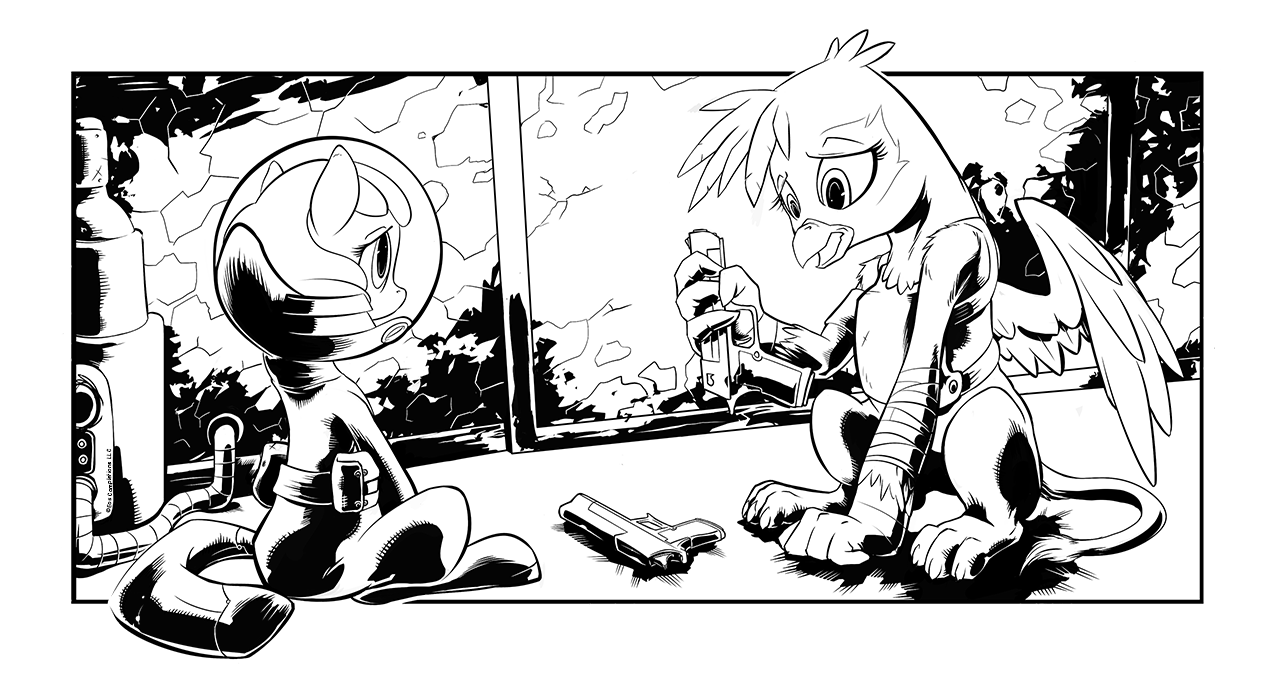
\includegraphics[width=\linewidth]{image06.png}


\begin{intro}
    Well, now, uh, Lancelot, Galahad, and I, wait until nightfall, and then leap out of the rabbit, taking the French by surprise - not only by surprise, but totally unarmed!
\end{intro}

{\rt Good evening my beautiful herd! This is Lonesome Pony and you're listening to Radio 52, the frequency that gives you all the essentials about Big 52 and nothing else!}

The evocative tinkling of Dueling Banjos filled a brief intermission.

{\rt Lets get to work. Have you ever wondered what the sun looks like? Ask the White Apples! Last night a gigantic ball of light exploded ten kilometers east of Salt Cube City bringing thunder and devastation in its wake. Luckily enough, along said wake there were mostly radigators and abandoned shacks, but the light could be clearly seen even from Tunnel Town, Badlands and the Redtrotters territory. If you think this is crazy, I must warn you that it was just the last act of a night of follies! First we had the launch of a balloon full of ghouls, yes the very same ghouls that threatened the caravans in the area! The take-off was accompanied by a light and magic show offered by a certain Puppysmiles. Weird name, isn't it? This is not the first time I've had something to say about this gal. Good old L.P. Asked some more questions here and there and guess what he discovered? Yes, she's the same filly from the Carnival!}

A trumpet erupted in a triumphant fanfare.

{\rt So, Lonesome Pony, where's the interesting part? Here it is for all those grumpy `too long didn't listen' busy ponies on the road: no more feral attacks between Badlands and the Cube!}

There was the sound of a reloading lever action rifle followed by pair of gun shots and a very manly voice saying ``Hasta la vista, filly.''

{\rt Oh yes I love this one! Two tribes get their problems solved by a foal stuck in a radsuit! Now I don't need to be a shaman to say that she's heading south, so\dots what's next? Is she going to reopen the Tunnel? Well kid, if you happen to stop by trade station Badlands on the Marshes detour, pay a visit to your number one fan! We'll get to know the filly inside the helmet! Till then, have some music from the best radio station you can find along the Route.}


\begin{song}
    Here's a pony there's a pony
    
    and another little pony
    
    funny pony party pony
    
    pony pony sprite
\end{song}

\horizonline

\englishdaytimeplace{5}{16:45 P.M.}{165Th Brigade field Headquarter, Salt Marshes}

``Stop that damn music, I can't hear if he's still outside!'' the young griffon snapped at Puppy while shooting her an exasperated glare.

``B-but it's funny! You are a grumpy chicken!'' The filly frowned and went back hugging her Pinkie Pie plushie, ``Don't worry Silky Tail: she's not mad, she's just a bit tired.''

Henrietta the griffon walked over to Puppysmiles and grabbed the filly's helmet so that she could look her in the eye. ``For the last time I am NOT a chicken! There's a freaking manticore out there that's pinned us inside this place and you are doing your worst to drive me crazy!'' The griffon's voice broke in a shrill screech. ``I hope that my father arrives soon,'' the girl sighed, ``maybe with his help we'll be out of here and I'll never ever need to see your stupid face again!''

``I'm not stupid\dots you are a meanie cat and I don't want to be your friend anymore!''

``{\mt Warning, Hostile griffon at three meters. Threat level: High.}''

``Aw, shut up mister Voice\dots'' Puppy turned her back on Henrietta in a theatrical display of sulking.

``Shut up mister who? Who are you talking with now?'' The griffon raised an eyebrow, ``You have a radio transmitter in that thing!?'' With a jump Henrietta was on Puppysmiles trying to take off her helmet. ``We can call for help! Call my father on 90.08! Codename Blaze!''

The filly was taken by surprise. ``Hey wait! I have to ask mister Voice! He lives inside the suit and works all the weird things!'' The foal tried waving a hoof to shoo Henrietta away but the griffon was already stepping aside.

``Wait. Mister Voice? That suit talks?''

``Sure it does! This is the best space suit ever! And it is also super smart!'' Puppy smiled proudly.

``Yeah\dots'' Henrietta snickered, ``I bet it's smarter than you.''

``Sure! Smarter than-'' the filly's smile became a frown, ``Hey! That's not very nice!''

The griffon was already laughing. ``I can't believe you fell for that! You're hilarious! Dumber than a banana pajama!'' Henrietta smiled and gave the filly a bump with her paw.

``H-hey stop that! You meany- mean chicken! If your dad wasn't that hurt I'd already given you a lesson!''

Henrietta froze in place, staring at Puppy. ``My father what? What do you know about my father?'' Hope and fear were mixing on the girl's face in a concotion that made even Puppysmiles aware that her next words needed to be used very, very wisely.

``Uh, last time I saw him he was dead\dots maybe he got better?'' The foal smiled, helplessly lost in childish naivete.

``M-my father\dots dead? How do you know that? Where have you seen him? This\dots this can't be, he's the best around he can't be dead! You're wrong this can't be true! Tell me that this isn't true!'' The griffin drew her white pistol and aimed at Puppy, the yellow line along the barrel pointed directly at her nose. ``Tell me that you're wrong!''

Puppy met Henrietta's wild gaze; the foal could be a bit slow, but there was no lie in those gleaming pink eyes, just the absolute innocence of a child. ``I\dots I don't know, he\dots wanted me to say to you that he really really wanted to be here and he was sorry. I ran here in a super hurry to find you because he was really sad and I felt bad for him and I lost my mom too-''

``ENOUGH!'' Henrietta batted Puppy's helmet with a claw, knocking the foal against a wall, before curling up on herself, trying to hide her face from the harsh reality. ``This isn't true\dots my dad is the best hired gun ever\dots he's okay, I'm sure he's heading here right now\dots fuck\dots I\dots I\dots.'' A soft metallic sound made the girl open her eyes.

Puppy stood in front of Henrietta; the foal didn't say anything, but took the black gun with the red line along the barrel from her saddlebag and left it next to the griffon before going back into a corner of the small room.

``Black Rose\dots'' The young flier stared at the gun in surprise as she came to realize what she already knew. ``Oh no\dots no, please\dots this can't be true\dots'' Again, she looked at the pony with the yellow suit, ``Please\dots tell me this isn't real\dots tell me this is a bad dream\dots''

Puppy frowned and looked down. ``I\dots don't know\dots if this is a bad dream then I'll wake up and find my mom waiting for me, so\dots I also hope that this is all just a really long bad dream\dots'' The foal sighed, ``but I don't think it is\dots''

``Fuck\dots'' Henrietta took the gun in a claw, looking at it and extracting her own .45 Auto pistol. They were identical in every detail but the color. ``How did it happen? Why were you there?'' \emph{Keep flying Henrietta, don't snap now. You learned from the best. You can do better, you MUST be better.}

``There were four chickens fly---''

``STOP CALLING US CHICKENS! We are griffins and we're better than you filthy ponies! Call me, or another griffon a chicken again and I'll make sure that it will be the last time! Capeesh?'' The griffon held Puppy by the neck, keeping her lifted off the ground while she pressed a gun into the filly's chest with her other claw.

The foal's eyes were filled with fear; Puppy tried to break free but after a quite useless struggle she simply gave up and began to cry. ``I\dots I'm sorry miss griffon! I'll behave! Please stop\dots please!''

Henrietta nodded and put the filly down. ``Way better. Now, there were four griffins. Where and when?'' That burst of anger somehow washed away the first shock, helping the griffin to focus a little more on the situation.

Puppysmiles talked fast, trying her best to not disappoint the scary griffon again. ``It was earlier: I was going down the road with a friend and they were in the sky\dots At the beginning it seemed that they were doing a pretty show, but then a lot of them got hurt and they fell from the sky and then they were all dead. I spoke with the last one before that he was dead and he told me to come here and give you that black thing and to say to you that he was sorry and that he wanted to go south and then I poked him to make him open his eyes but he kept sleeping I tried really hard to wake him! Please don't be mad at me I really really wanted to make him get better but he didn't move and then mister Voice told me that he was dead and\dots and\dots'' The filly stepped back, gasping for air and putting both hooves above her head in an attempt to hide herself. ``Please stop bullying me I didn't want to be mean I just wanted to help! I'm sorry!''

\emph{Fuck, she's just a kid.} The griffon hesitated as her anger began to fade. That foal probably didn't even mean chicken as an insult\dots nonetheless someone had to teach her something before she got into real trouble.

``And guess who's that someone\dots'' muttered Henrietta, sighing; the half-eagle patted Puppy's helmet, ``It's cool, really. Call me Henrietta or Henry, okay? You just lack some\dots style; but don't worry, you'll learn. Now let's find a way out of here.''

``But\dots but you are mad at me\dots'' Puppy was still hiding her head behind the hooves.

``No, I'm not mad\dots now be a good pony and stand up, okay?''

``But I called you a chicken and I told you that you were mean\dots'' protested the filly.

``Just don't do that again, okay? I scolded you and now we are even\dots alright?''

``So\dots so we can still be friends?'' tried hopefully Puppy.

The griffon sighed. ``Yes, we can still be friends\dots now please be quiet while I think up a plan.''

Yes, sure, it was easy to say\dots maybe a little harder to achieve, but even those simple words were enough to renew Puppy's happy-go-lucky mood. The filly nodded and sat next to the stairs, while the griffon took a look outside; the predator had to be hiding somewhere, probably waiting for them to venture out in the open.

``Not good\dots if only I had something better than my guns. I could hope for a lucky shot, but if it doesn't work\dots'' The griffon looked back at Puppy, ``Hey, you don't happen to have a big caliber gun or some high explosives, do you?''

``I have a rock! It's super rocky!'' Puppy proudly showed \emph{The Rock Of Destiny} to Henrietta.

This made the Griffon snicker. ``Oh yes, exactly what we need: a rock. Sorry kid but I don't think that I'll let a stupid rock decide my fate.''

The filly tilted her head, then looked a bit confused at her favored weapon. ``I don't think that you're dumb, Rock\dots but now it's better that you go back sleeping.''

``Please! I'm trying to put a plan together here. Stop kissing goodbye to everything you stash in your saddlebags and do something useful like\dots'' Henrietta hesitated, ``Like\dots ah\dots On second thought, just go back and play with Twinkle Sail.''

``Silky Tail!''

``Yeah, that one\dots have fun\dots''

``Okie dokie! The tea will be served in five minutes!'' Puppy sat down on the stairs taking the stuffed Pinkie Pie from her bag.

``Yes, whatever\dots now\dots'' the griffon lowered her voice to a mumble: ``there's no decent cover and I'm not sure that I can outrun that thing for more than a couple of minutes. We have to face it, but we lack the firepower\dots'' Henrietta sighed in distress, ``this is ridiculous: those tanks are full of high explosive ammunition and we are stuck here with three .45s and\dots a rock\dots''

In the meantime Puppy sat her doll on a large Flack 8.8 projectile while using another one as a teapot to serve tea. ``Hey, do you want six or eight sugar cubes in your cup? Ah\dots do you have a cup?''

``No thanks. I think I have a plan,'' the griffon said without even bothering to turn back to the foal. ``I'll run outside trying to get the manticore's attention. After the manticore starts chasing me you'll sprint to the nearest tank and get inside; you have to be fast because I can't distract that thing for very long. When you're in the tank you have to look for HE ammo: they're big and shiny, like a big can with a pointy head; they should have a red band so they are easy to identify. Alright?''

``Uh, yes\dots'' Puppy looked for a moment at her 'teapot' shrugging and putting it away, ``You just keep an eye on Silky Tail, okay?''

``I don't think that your doll is going anywhere while we're out. Just go inside the tank, grab the big can with the red line and run back here; when you're done I'll explain to you the second part of the plan.'' The griffon crouched, readying herself for a jumping start: she needed all the speed she had.

"But she will be afraid!'' That filly was a constant source of idiocy and distraction.

``Puppy, Twinkle Sail is just a doll! It can't be afraid!'' Henrietta walked over to the stuffed Pinkie Pie/Silky Tail, grabbing it and waving it around in front of the filly: ``See? She is smiling, so she is okay! Maybe when we are back she will throw us a\dots HE Flack 8.8?'' The griffon's eyes focused on the object being used as a chair for Puppy's toy, ``Pardon me\dots where did you find this?''

The filly in yellow smiled. ``Soft Air gave me Silky Tail in the Glow.''

``No, I mean this one: the 'chair'\dots''

``Oh that\dots it was inside a broken super huge metal cart; it's shiny and clean, I've got plenty of them.'' From the expression on the griffon's face Puppy felt that she had to say something more. ``Do you want one?''

Henrietta's left eye went twitchy twitch. ``Okay, great\dots part one done\dots now part two\dots''

``What? But we didn't even-''

``No\dots just\dots no. I said part two, let's never speak of part one again.'' The griffon's self control was considerably improving. ``Listen carefully: I'm trying to lure mister Big Bad here at the tower entrance: when the manticore pokes his head in you have to throw the shell into his mouth and then I'll shoot it. The head goes boom and no more bullies, got it?''

Puppy frowned. ``So\dots I throw the teapot inside the jaws and the movie ends?''

``The what? Yeah, sure: throw that thing in the manticore's mouth and I'll do everything else. Now get ready and don't be scared, Okay?''

``Okie dokie!'' The filly hugged the shell and hid herself behind the wall while Henrietta cautiously stepped out of the building with her wings outstretched.

Not even a minute later the sound of gunshots came from outside, followed by the voice of a griffon who was teasing the manticore with a lot of words that Puppy never heard before. The foal was super double curious about what was going on outside, but she had been told to stay put and wait. Now this was a dilemma: if Henrietta found her out of place she was going to be really mad and that girl was really scary when she was mad\dots on the other hoof Puppy was sure that there was something totally cool going on just a few steps away from her.

``Maybe just a little peek\dots'' Outside it was raining lead while roars thundered in the storm of the battle. ``Just one\dots It won't hurt, right?'' The filly slowly crawled next to the door, always hugging her HE shell and trying to look outside, ``Sneaky sneaky\dots''

``Aw, I can't see a thing! This isn't fair at all-''

Suddenly a blurry silhouette came speeding through the door, rushing to the opposite side of the room and yelling ``NOW!''

``Now what?'' asked Puppy a little surprised.

ROAAAR!

Snarling and scraping at the concrete, the manticore appeared at the door, trying to get inside but being held out by it's size. Puppy found herself looking into the snapping jaws of a fell beast just a few inches away from her helmet and yelped backpedaling.

``What are you doing Puppy! Throw that thing now and dive for cover!'' The urgency in Henrietta's voice danced with the panic in her eyes. ``Move that cutie mark!''

The filly in yellow nodded and tried launching the shell: the high explosive round described a straight trajectory through the air while Puppy jumped as far away as she could. When the explosive ammunition hit the ground right below the beast's head the griffon opened fire.

BLAM! BLAM! BLAM!

Three shots, three hits, three bounces. ``Fuck! It's case is too thick, I can't penetrate it!'' The gunslinger girl swore and emptied both pistols against that stupid explosive shell with no avail.

``It's not working!'' Henrietta put away one of her guns and took a third pistol. This one was Red with a white line along the barrel but in everything else it was identical to the other two she had. Unloading the gun directly in the manticore's muzzle she succeeded in making the monster slow down his assault for a moment.

``I think he's trying to make the door larger.'' Puppy stepped back another couple of meters but now she seemed a lot less scared. The foal tapped her helmet as if she was pondering the situation. ``He's good\dots''

The beast was looking at Henrietta with bloodlust in his eyes; it was clear enough that he wasn't going to lurk any longer even if this meant tearing apart the whole tower. The real issue was that the manticore was actually tearing the building apart: maybe not very fast, but he was getting there.

``Don't just stand there! Come here!'' The griffon reloaded her pistols, ``We can still make that thing go boom if only I can hit the detonator. You just stay low I'll try something!''

``What's a dee-tuna thor?''

Henrietta launched herself towards the manticore ignoring Puppy's question. With a leap she arrived just a couple of slashes out of the beast's reach and pointed both guns at the shell. ``Say goodbye Josè-'' Too late the young fighter noticed that the predator had his head reclined and his back arched. Henrietta was half feline too, she had to know how much a manticore can stretch; she should have known better, but now the cat had just fallen into the lion's jaws. He didn't even give her time to swear.

In that moment the manticore stretched out and struck the griffon with a claw, hitting her in the shoulder and grabbing her with his mighty talons. Henrietta shrieked in pain and instinctively but uselessly pecked and bit at the monster's paw.

Puppysmiles screamed in terror, too. The filly tried to back away further but her rump was already pressed against the wall. This manticore was terrible but even worse, he was hurting Henry.

For a moment Puppy didn't see the manticore but a pink metal face with blinking blue eyes.

\emph{Please -giggle- make this -giggle- end.}

Puppy's eyes flared with pink flames while she raised a hoof. ``Rock!'' As soon as \emph{The Rock Of Destiny} was in her hoof the filly launched herself against the beast. ``Let her go! Let her go NOW!''

The manticore immediately spotted the yellow critter assaulting him and instinctively turned his head and closed his jaws on her, tossing his old prey aside. The fangs of the monster closed on the little filly, crushing her with a dry crunchy sound. Henrietta fought to stay conscious while she staggered across the room trying to reach the stairs. In the meantime the manticore let out a triumphant roar that sealed once and for all Puppy's fate.

``No\dots no, it's too late\dots Save yourself gal\dots don't turn back\dots'' Weakly, the wounded griffon climbed a couple of steps but the pain was driving her crazy. The manticore behind her was howling in a bloody ponycidal rage, probably tearing apart and dismembering every limb of that poor corpse. Henrietta took a healing potion and swallowed it in a single gulp, then fell face down as her sight began to fail her. Henry tried to turn over to see what was going on and why that atrocious beast kept roaring and howling, but all she could see was a thick pinkish smoke and nothing else\dots then the griffon lost her battle against the staggering pain and fainted.

\dots

% NOTE: change the order

Now please let's have a minute of silence in memory of a truly unfortunate manticore.

And this is why rule number one says no biting. Never. It could be spoiled.

\horizonline

\englishdaytimeplace{6}{00:45 A.M.}{165Th Brigade field Headquarter, Salt Marshes}

``{\mt System successfully rebooted. All functions restored. Diagnostic system is online. Subject 001: Puppysmiles. Female earth pony. Subject deceased, condition stable. All clear.}''

Puppy lazily opened her eyes and yawned. ``But it's still dark outside\dots'' She had the unpleasant sensation of something heavy laying on her back. ``What happened? Where's the chicken? And the big meany kitty cat?''

``{\mt Analyzing. Hostile detected. six meters east. Henrietta. Threat level: negligible.}'' A single red dot was blinking on the compass.

``Silly Voice, Henry is not an enemy\dots'' The dot turned pink. ``Okie dokie, let's go to\dots hey!'' The filly moved her hooves but this didn't make her go anywhere. Puppy looked down to see that she was hanging from some sort of gray perch. It took more than a couple of tries to break free from the skull of the manticore; the skeleton of the beast had turned the same color as the wall and seemed to be partially stuck inside it as if the animal and the wall had melted together. The large head full of teeth was open in an eternal roar while his wings stretched out, desperately trying to break free from the deadly cloud that had consumed him.

Puppysmiles trotted over to Henrietta but the griffon was lying on the stairs giving no signs of life. ``Mister Voice, is she\dots you know\dots uh\dots dead?''

``{\mt Analyzing. Negative. The subject is unconscious.}''

``Oh\dots This means that she will be okay?''

``{\mt Affirmative. The subject is recovering.}''

``Okie dokie.'' That was enough for Puppy: she smiled and kissed Henrietta goodbye through her helmet, ``I'm sorry but I still have to go, chicken girl. My mom is somewhere on the other end of this arrow.''

Puppy trotted some meters away but then stopped and frowned: somehow she felt that just kissing goodbye this time wasn't enough. The filly went back to Henrietta, took the Pinkie Pie doll from her saddlebags and put it under one of the griffon's paws.

``Here, Silky Tail. Look after Henrietta and don't let anything bad happen to her.'' Now it was really okay. Puppy trotted outside and retrieved her scooter.

``Hey, can I has some music?''

\begin{song}
    In the jungle, the mighty jungle,

    the lion sleeps tonight

    in the jungle, the quiet jungle,

    the lion sleeps tonight
\end{song}

\horizonline

\englishdaytimeplace{6}{10:00 A.M.}{Griffon's Fall, Salt Marshes}

Digging in a marsh without a shovel was already torture by itself, but digging your father's grave in this muddy terrain with your bare claws was\dots No. Just, no.

Tears dropped from the griffon's beak while she swallowed pain. Every time she tried deepening the hole in the dirt it was filled again with murky water but she kept digging in silence. He could never bear her crying, he was the most hardened badass mercenary ever. And now he was dead, killed by Talons.

Henrietta dragged the dead body to the shallow hole and pushed him inside; the corpse settled into the mud with a gurgle. The daughter watched the blood stained feathers sinking in the pool and tried her best to fight back the tears. Fuck\dots he wouldn't even sink in completely.

``Not fair man, leaving me alone like this\dots what am I going to do now?'' Henrietta sighed; she tried being mad at him if only to find a weapon against grief, but it was so hard. He was gone\dots so what now? ``Why you\dots''

Fuck.

Just fuck.

The griffon began filling the grave again with mud and all the stones and asphalt chunks she could find nearby. With the last stone in place, Henrietta stared at where his beak had been visible just moments before; she took out the black gun and hesitated, then put it away again. Instead, she plucked three feathers from her right wing and planted them where she knew her father's chest would lie forever.

``Tell mom I'll be fine, okay?''

Henrietta rubbed her eyes with one claw while she rummaged in her bag with the other, retrieving Silky Tail. The griffon looked into the smiling blue eyes of the stuffed doll and tried to smile back. ``I'll be fine.''

\horizonline

\englishdaytimeplace{6}{11:30 A.M.}{Random encounter location, Salt Marshes}

``Hi! I'm Puppysmiles!''

One of the three slavers, a black earth pony, frowned. ``I think I heard that name before\dots Maybe we should just pass on this one\dots'' He looked at the other two ponies: they were all well armed but over the last two days Lonesome Pony kept rambling on about a ghost infesting the northern branch of the Big 52.

``I'm not afraid of ghosts, Dripping Blood. But if a foal scares the shit out of you then just keep an eye on the other slaves.'' The leader of the slavers, a yellow unicorn, glared at his meager haul: a couple of stallions and a foaling mare\dots way below the quota, ``Forty Nails, Catch her.''

Puppysmiles was a bit uncertain: there were six dots on her compass but half of them were pink and the other half was red\dots this had to be another weirdness by mister Voice. One of the ponies marked with a red dot approached her cautiously and put a hoof on her back.

``Now come with us and don't resist, kid.''

``Okie dokie! Where are we going?'' The filly in yellow smiled with enthusiasm.

Apparently her behavior was quite odd to these newcomers. The nearest pony, a green unicorn, looked over to his boss, who shrugged and encouraged him. ``See? Easy peasy. Put her in a collar and let's move.''

Forty Nails tried to open Puppy's Suit but he wasn't exactly a Ministry of Peace technician. ``Hey boss, this fucking thing won't open!''

``U-uh. I can't take it off too: it's a super stuck helmet\dots I even tried hitting it but it just keeps repairing itself\dots'' At last somepony was helping Puppy with the space suit problem, but they didn't seem anywhere skilled enough. ``I think that there is some sort of button to press here and there but they don't work\dots''

``Shut up, retard.'' Forty was losing patience and decided to go medieval on the whole problem: ``It's clobbering time.'' he held up a hydraulic wrench and brought it down hard on Puppy's helmet, creating an intricate network of cracks that ran across its surface.

The yellow unicorn roared. ``Hey if you break her head I'll break yours! A dead foal is worth nothing!'' The black slaver simply kept an eye on the other three slaves snickering at the scene.

Puppy stepped back, afraid. ``Hey that's dangerous!''

``{\mt Warning. Compass malfunctioning. Warning. Sensor system offline. Warning. Helmet integrity severely compromised. Repair system activated.}''

``Fucking Sun, that's a hard nut to break!'' The green unicorn raised his weapon again only to see that the cracks in the helmet were already closing, ``What the fuck?'' He hesitated.

``Just tie her up with a rope and let's get going, we'll see to that once we're out of this shit hole.''

Puppy was told to behave, so she behaved while the pretty ponies put a noose around her neck. It was only when they tried dragging her with the other slaves that she began feeling something wrong in the air.

``Hey, I can't leave my ride there!'' The filly trotted towards her scooter but the slaver holding the rope stopped her with a sudden jerk.

``Where do you think you're going?''

Puppy kept struggling. ``My scooter! Lemme go!''

Forty Nails snickered. ``Yeah sure, bitch.'' He pulled the filly close and looked into her eyes: ``You're a slave now. Forget your scooter and everything else. If you want to stay alive, stay put. Got it?''

``Uh\dots but I have to go there!'' Puppy pointed a hoof south. The green unicorn snorted and hit her on a flank with the butt of his hunting rifle.

``Shut up and open your ears or I'll rape you hard! Rebel ponies are bad commodities anyway.'' Forty turned to the slaver's leader, ``Hey boss I'm teaching this one a little respect''

``Don't mess her up or you'll be paying for her.'' The leader shrugged without even turning back.

The filly in yellow frowned. ``I don't think that's a nice word\dots'' She seemed completely unfazed by the first beating so the green slaver gave her a stronger blow.

``SHUT! UP!''

Puppy was sent flying, landing a few meters away. ``Hey! somepony could get hurt!'' She got up on her hooves giving no sign of pain and earning a worried look from Forty Nails

``B-but\dots what are you? Fuck off and stay down!'' The slaver aimed his rifle and shot two bullets into the foal.

BLAM! BLAM!

Two hits, two holes in the filly's chest and still no reaction from her. Forty's eyes widened in terror. In the meantime the leader turned on his minion.

``What the fuck are you doing you fucking son of a fucking drug addict! This is the last time you kill a slave!'' The yellow unicorn charged the green pony head down, sending him flying through the air.

``No! I'm not gonna die here!'' In a state of utter panic, Forty turned his rifle against his boss and emptied the magazine; one of the unicorn's legs exploded before he could even realize what was going on. The slave leader fell to his knees, pulling out his assault rifle and spraying bullets all around. The black earth pony that had kept silent until now unsheathed a shotgun but was hit by the raging boss along with one of the slaves and Puppysmiles. The bullets pierced the foal leaving at least three different holes but it didn't seem to affect her very much.

``Stop quarreling! Please! Hey! I'm talking with you too!'' Puppy tried to restore some order but this brawl seemed a bit beyond her capabilities. ``You are all bad ponies and you should feel bad! Mister Voice, do something!''

``{\mt Repairs finished. Containment fully restored. Subject 001 Puppysmiles deceased. Condition stable. All clear.}''

``Not that something! Something else!'' Puppy pouted.

The black slaver staggered trying to retrieve a healing potion but the unwounded stallion slave rammed him, taking his gun and emptying it into his sorry muzzle. The wounded slave fell on the ground coughing blood while the pregnant mare tried to find cover behind the armed slave.

Forty Nails exhaled his last breath and even the leader was rapidly bleeding to death; but he didn't want to hit hell's doors alone. With a glow of magic a remote control appeared from his saddlebags while he coughed blood trying to laugh. ``Do not fear -cough- little ponie -cough- ponies\dots you are going to -cough- to precede me\dots'' He raised his good hoof to hit the detonator for the the slave's collars. The two surviving slaves looked at him in horror.

``No toys for the meanie pony!'' A yellow hoof took the detonator from under the slave leader's muzzle. Puppy was looking at him with her best scolding look. ``I said stop being crazy! I'll keep this thingie until you behave!'' the filly gave a theatrical pause, ''And I'm dead serious about this.''

The slaver looked at Puppy and snickered. ``I\dots can't believe this\dots -cough- I heard that story about -cough- the ghost\dots'' His eyes focused for a moment on the last scratches of Puppy's suit as they disappeared completely, ``Hell\dots you're\dots -cough- fucking scarier -cough- than I could -cough- could ever ima\dots gi\dots n-\dots'' The slaver's voice died as his life dripped away into the thirsty wasteland.

\horizonline

\englishdaytimeplace{6}{8:30 P.M.}{Tunnel Town Outskirts, Big 52 N Branch}

``So, when mommy pony loves daddy pony super special much they write a letter to Princess Celestia and ask for a little foal. You really didn't know that?'' The filly trotted and galloped all around as she talked.

It had been a long, but luckily uneventful walk through the salt marshes. At last the endless plain of murky pools was behind them, giving way to an area of barren hills. Now it was possible even in the darkness of the night to see any suspect movement from a good distance. Puppy's HUD flashed here and there with red dots, but they were mostly wild animals scared by the filly's supernatural presence.

The pair of ponies traveling with Puppysmiles were in a bit of distress. It was the pregnant mare, a milky unicorn by the name of Sweet Flower, who spoke first: ``Well yes, it works more or less that way\dots you're quite a chatty filly, aren't you?''

``Yup! Everypony keeps telling me that.'' Puppy smiled and completely changed the topic, ``I hope that you get a filly. Fillies are the cutest!'' She lowered her voice, ``Besides, I heard that colts have cooties! It's true!''

Sweet Flower giggled and nuzzled her companion, a brown earth pony named Asso, in the neck. ``She's a little bit right, isn't she?''

Asso laughed. ``I just know that it's going to be awesome.'' The stallion stopped trotting and looked in the distance.

``Here we are, little one: that's the Tunnel.'' The brown pony pointed a hoof to a small group of lights perched on the middle of a steep mountain wall.

A large bridge, formed by many stone arches rose from the swamp, climbing directly toward the mountain like a highway to the sky. Puppy's eyes widened in awe at the sight of such a marvelous thing: it seemed like the road shot upwards like an arrow of awesomeness and then BAM! It disappeared in a show of colored lights. The filly's two companions were way more interested in her: the foal's eyes shone in the dark, a bright pink light that surrounded the helmet in a ghostly halo.

``Okie dokie! So, we go now? Mom is waiting for me somewhere in there!'' the foal asked enthusiastically and epic failing to notice the alarmed looks the two gave each other.

``Ah\dots well, we don't live there and you need to pay a fee in order to get inside Tunnel Town. We are heading to trade station Badlands: it's a small hub along the detour.'' At that point Asso hesitated but the mare nudged him, encouraging her mate to speak his mind. After a brief pause the stallion lowered his eyes and continued. ``I\dots we have to know this: are you really a ghost? Some sort of guardian angel sent here to protect children?''

Puppy tilted her head and giggled. ``I'm Puppysmiles, mister pretty silly pony! I don't know why everypony keeps calling me a ghostie but I'm just looking for my mom.''

``Yes you\dots you told us that about a million times\dots'' Asso gave a tired look at his mate and shrugged, ``Well, I guess this is all. We owe you our freedom, somehow\dots so\dots Thank you? I wish I had something to repay you but we need everything we have just to get home alive.''

``Okie dokie! Goodbye pretty ponies!'' Puppy waited until her new friends disappeared from sight then merrily trotted up the bridge towards Tunnel Town.

~\vfill

\begin{engnote}
Level up! (5)

New perk added: Intense Training (2) - Strength ($5 \to 6$) You can has a lotta stuff in your bags!
\end{engnote}





\chapter{Foalsitting}

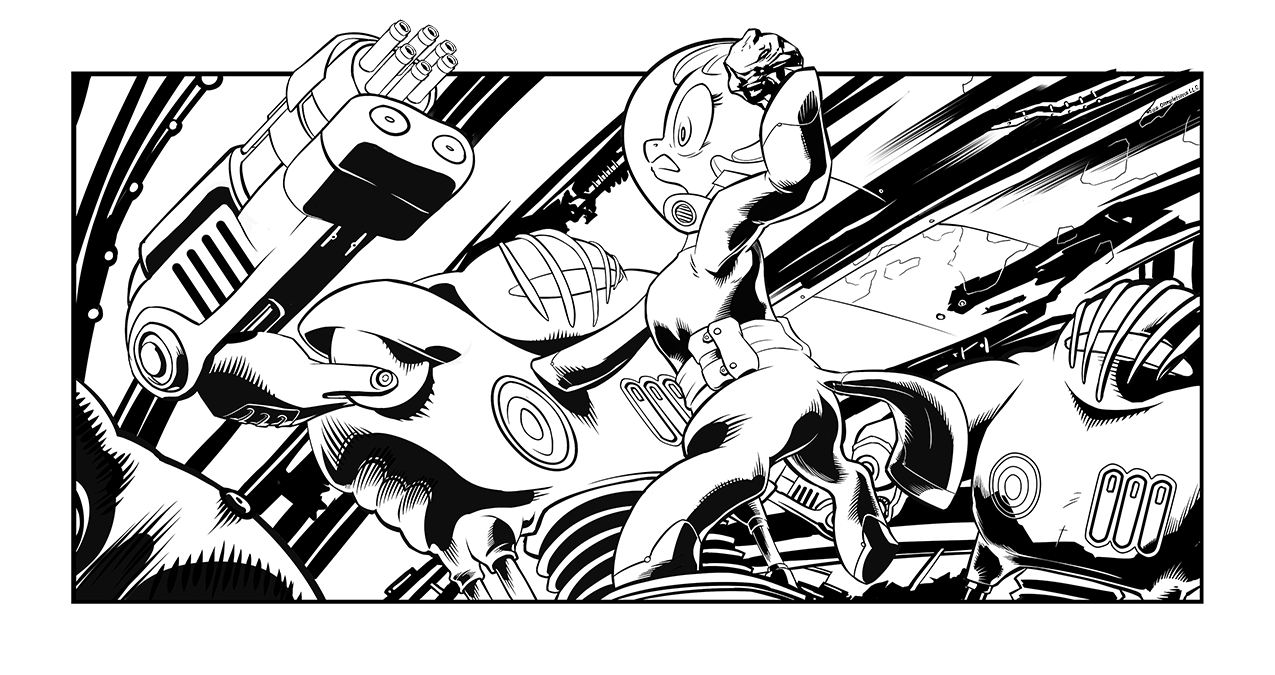
\includegraphics[width=0.9\linewidth]{image07.png}

\begin{intro}
What? These sweet little angels? They'll be no problem at all.
\end{intro}


\englishdaytimeplace{6}{9:00 P.M.}{Tunnel Town, Big 52 N Branch}

Trigger Happy had been a guard for a good half of her life, and she was pretty sure she'd seen everything that could try to get through the Tunnel Town gates. Tonight, she had to admit that she had been wrong, but the fact that all her guards were cowering behind her because of a foal in a funny costume was even more upsetting.

``All right, scaredy-ponies, I'm taking this one. Just relax and, for the sake of my sorry tail, don't shoot blindly.''

She stepped out of the guard post and trotted toward the yellow foal who was surrounded by an eerie pink light. ``Okay, that's close enough. Stop right there and tell me what the hay you are!''

Trigger didn't actually expect the foal to comply, but when she sat down the guard chief felt relieved.

The strange pony rose its hoof and waved it at her. ``Hi! I'm Puppysmiles! Have you seen my mom?''

Trigger Happy frowned. ``Puppysmiles as in 'Puppysmiles the ghost'?''

``I'm not a ghost, I'm a filly!'' she protested. She was carrying something long and red strapped on her back. It didn't seem a weapon, but it was still quite large.

``Let me guess. You zoomed all the way here from Salt Cube City through the marshes on a Red Racer?''

Puppy giggled. ``Nope, I had to trot a bit because the fat unicorn was super boringly slow.''

``The who now? No wait! On a second thought, I don't care.'' Trigger sighed. ``Now I'm coming over. You just don't do anything, ah, ghostly.'' Trigger turned her head toward the guard post just to meet three pairs of eyes that were carefully hiding behind the barricade. One of her guards waved a little white banner for a second. She silently wished for a crew that was less stupid, then trotted toward Puppysmiles.

``Hi! You're pretty, miss pretty pony! What's your name?'' The foal smiled her friendliest smile.

\emph{It's\dots it's just a filly with a pair of glowing eyes, probably caused by a mild case of radiation poisoning.} Trigger chuckled. ``Are you serious? You're the Puppysmiles from the news? The one from the Carnival and Salt Cube City?'' She laughed. ``Oh please, gimme a break!''

Puppy smiled and laughed too. ``Ah ah ah! That's funny! Uh, why are we laughing?''

At Puppy's question the guard chief laughed even louder. ``Name's Trigger Happy, but you can call me Trigger.''

Puppy frowned. ``Ah, can I call you Happy?''

``Sure. Anyhow, I have something for you.'' Trigger took a yellow piece of plastic and handed it to Puppysmiles. ``Here's your pass. A griffon by the name of Henrietta was here at noon. She waited until dusk for you, but then she had to move. Before leaving, she bought you the ticket saying that you were arriving sometime tonight or tomorrow.''

``Uh, Henri was here? Was she all right?''

``Yes, I think. She wasn't very chatty, but I never met a chatty griffon.'' Trigger turned on her tail and trotted back to the guard post. ``Come in! Staying outside this late is unhealthy. We have some bloodwing issues 'round here.''

``What's a bloodwing?'' Puppy asked, trotting behind Trigger.

``If you ask me, they're trouble. Think of them as large flying leeches.'' She snickered and beckoned Puppy inside the guard post. It was a low building surrounded by sandbags and rusted plates of metal. A couple of miniguns were placed in front of the windows overlooking the bridge, and there was a stack of ammo boxes stashed in a corner. Three ponies greeted Puppy with scarce enthusiasm as she followed the mare inside.

``Look alive guys. This is Puppysmiles, the hero of the Carnival. As far as I know she's on our side, so we have nothing to fear.'' Trigger snickered. ``I'd give my cutie mark to see how Lonesome Pony would react if he knew what his \emph{'hero'} really looked like. Anyhow, this is Green Pear, Jammed Gun, and Little Bean.''

``Hi, I'm Puppysmiles!'' She trotted toward the trio of ponies. Since her new friends seemed a bit uneasy, she felt that something more had to be said. ``I'm looking for my mom, and she's somewhere inside the mountain!''

One of the three guards raised an eyebrow and mumbled, ``Well, that could be a problem.''


\horizonline

\englishdaytimeplace{6}{9:45 P.M.}{Tunnel Town, Big 52 N Branch}

``Wow, it's huge!'' Puppy sat in front of the tunnel entrance. It consisted of a large archway high enough to let in both ground carts and air wagons for emergencies or maintenance. The entrance was so wide it could have handled passage from both directions at once. The concrete of the tunnel walls ended abruptly twenty meters into the mountain, where a rusted metal bulkhead sealed it. On the door there was the symbol of a white alicorn, but this one seemed more bulky and manly than the goddesses. Around the symbol ran a motto: \emph{Solaris Inc. ‒ Try the alternative.} Under the company slogan there was a big red symbol, suggesting danger, that occupied most of the door.

``See?'' Trigger Happy knocked at the metal door a couple of times. ``It's sealed. I'm afraid that your journey ends here, little one.''

``But my mom is in there! Look at the arrow, see? It points to the door! I have to go inside the mountain! Open it please!'' Puppy put on her best pout. ``Puppy please, Miss Happy pretty pony?''

Trigger stepped back frowning. ``Wow, those eyes should be classified as illegal military ordinance! Still, I'm sorry, Puppy. There's no way inside the Tunnel. We have tried our best to reopen it, but, as you can see, it won't budge.''

``But I really, really, REALLY have to go there! My mom is waiting for me!'' She stubbornly stomped her hooves.

Jammed Gun tapped his chin with a hoof and muttered, ``I think that TNT once said something about getting inside using the vents.''

Trigger's eyes widened. ``Shush!'' She launched an angry stare at her subordinate before quickly turning back to Puppy, trying to hide a concerned look under a fake smile.

``See? No way inside!'' She tried to hold a poker face, but Puppy was already frowning.

``Uh, vents? What are the vents? Please, I'll do anything. I-I have this!'' Puppy produced one of the tank shells from the military base. This one had a black band around its head. ``See? It's shiny and super duper nice! You let me go inside and I'll give it to you! Deal?''

``Puppy, it's dangerous. I can't let a foal trot to certain death! I'm sorry.''

Puppy stepped back, on the verge of tears. ``I'm not afraid and you're unfair! If it was your mom that was closed inside, you would already be opening that stoopid door! And\dots and---'' She bucked the door. ``I can't stop now! She is there, she \emph{must} be there!''

Jammed stepped next to Trigger and whispered, ``Why not let her in? After all, she's already saved two towns! Besides, I don't think she's just a foal.''

Trigger sighed before she replied. ``We don't know what's going on inside the Tunnel right now, but I'd like you to recall the day the door closed. I clearly remember the ponies trapped inside hitting the door and asking for help, the sound of the guns, and the voices screaming in pain and terror.'' Trigger softly bumped Jammed's forehead with a hoof. ``Look at her. Maybe she's not your average little pony, but she's still just a kid. I'm not sending kids to clear minefields.''

Jammed looked into his chief's eyes. ``Do you think that she'll give up that easy? If she really is the famous ghost, I don't think there's anything we can do to stop her.''

Trigger Happy facehoofed. ``Are you really falling for those fairy tales? Please, get real! She's just a filly with a full enviromental suit and mild radiation poisoning!''

In the meantime, Puppy was still standing in front of the door, muttering to herself. ``I'm not a foal, I'm a big pony! I've made a balloon fly!'' She frowned angrily at Trigger Happy. Suddenly, a new idea popped into her head, making her smile cunningly. ``Say, Mister Voice, what is this vent they are talking about?''

{\mt ``Vent: ventilation system. Device used to circulate fresh air inside close spaces. In the case of a tunnel it consists of a long web of passages that take air from the outside and pump it inside using fans and small ducts large enough to let a single pony crawl through them for maintenance--the more you know!''}

``So, ah, there are other doors to go inside the mountain from where the air gets in?'' asked Puppy, trying to translate what she was just told.

{\mt ``Affirmative. Loading local maps. Solaris Inc. Tunnel n° 2. Analyzing technical blueprints. Warning. Part of the blueprints are not available due to military restrictions. Loading section A01, A02, and A03. Loading maintenance tunnels blueprints. Analyzing. Elaborating route. Maintenance hatch A01-104 set as new waypoint.''}

The pink arrow disappeared from the compass and appeared again pointing to a new direction.

A grin appeared on Puppy's muzzle. Once again she had outsmarted her rivals.


\horizonline

\englishdaytimeplace{6}{10:15 P.M.}{Tunnel Town, Big 52 N Branch}

``And I'm saying that I've never seen a pony survive inside a sealed suit for more than three days! Your 'kid' seems just a bit too fine to be normal!'' Jammed Gun pointed a hoof at the empty place where Puppy was supposed to be. He did a double take, looking at where he was pointing and realizing that something was missing. Something the size, shape, and color of Puppysmiles. ``What the hay?''

Trigger Happy jumped on her hooves, looking around frantically. ``She was here a minute ago! Why didn't you keep an eye on that filly?''

``Oh, now \emph{I} have to watch after the glowing, yellow pony? And what were you supposed to do?'' Jammed stopped and snickered. ``See? It's just like I was saying, you can't stop the Ghost of the Big 52.''

``She's not a ghost, so stop blabbering.'' Trigger Happy waved a hoof, dismissing the idea, but her companion continued talking.

``Now please, Happy, listen to me for a moment. This place is getting worse every day. When we were kids we used to play outside, and the Big 52 had way less slavers and bandits. The tribes were strong enough to keep order and make everypony feel a little safe.'' He sighed. ``Don't you miss those days, Happy?''

She looked down, sadness filling her eyes with a dim shadow of tears. ``Yeah, but at that time it was easier. The tunnel was still open, and Sun City was a civilized place. Now the Big 52 is just a bunch of detours and dangerous trails.''

``Yeah, I know\dots so I was wondering. They say that everything has a spirit, right?'' Jammed Gun was trying hard to explain a thing that was quite clear in his head, but not that easy to put down in words. ``It's like a city. A city is more than the ponies that live in it. The efforts of the community and the hopes of the families sustain each other, feeding a common will that makes you feel as if the whole place is alive.''

``Yeah, it's called community. So what?'' Happy looked at Jammed with a dubious expression. ``I hope you're really going somewhere with this, because we have a lost filly right now!''

``So, even the Big 52 is something like that, right? I mean, The Redtrotters, the White Apples, the Sand Sweepers, and all the other tribes. Maybe they're separated, but they all live on the same long route from the Ridges to Emerald Shores. We are all on the same road, and we all are citizens of the Big 52.'' Jammed Gun raised a hoof pointing north, then arched to the south with a slow movement. ``Salt Cube City belongs to the White Apples, yes, but the Big 52 belongs to everypony that lives along it.''

``This is a very poetic idea, but I still don't see how this is going to help us find Puppy.''

``I'm almost there. We both had that feeling. You know, that the Big 52 is dying. Slowly but inexorably sliding into the same horrors as the rest of Equestria. And suddenly\dots bang! This Ghost appears and starts solving problems that vexed us for years.''

``The Redtrotters were slowly giving up. The Carnival was killing more than a foal per year. It was killing hope. Once I heard a trader say that the mares of the tribe refused to have foals because they were scared to lose them. And the ghouls? Do you know how many caravans traveled only as far as Exchange Station Badlands because making the trip to Downtown wasn't worth the additional escort?''

``Well, yes, okay, but I don't think that a foal can---'' 

``And I think she can.'' Jammed was dead serious. ``Think about that griffon today. Have you seen her eyes? She had this\dots light. As if things for her had sucked for a lifetime, but finally they were beginning to get better. She had hope, and she showed gratitude. Think about this, Happy. How many ponies in this sinkhole value gratitude? Maybe several years ago it was still common to think of other ponies as something other than a potential threat, but nowadays if you don't have the pass you aren't even given a chance.'' Jammed paused for a moment, but now Trigger was listening carefully and didn't interrupt him.

``And now she needs to get into the Tunnel. Maybe she is just a lucky foal, or a dead one, but---but I want to believe that she's something more. Okay, maybe she's not the Stable Dweller, or Security, but she's all we got down here. Just the good old Big 52 trying to fix things by herself.''

Trigger Happy sighed. ``You are a dreamer and a silly pony, Jam. If you have a problem you can't just wait for somepony else to come and solve it for you. You have to face it and work hard in order to earn something.'' She looked away at the ever-clouded sky. ``But I have to admit that in one way, you're right. That filly doesn't know when to give up. I think I know where she's headed, and Luna curse my soul if I'm letting her wander into trouble.''


\horizonline

\englishdaytimeplace{6}{10:15 P.M.}{Solaris Tunnel, Tunnel Town}

A metallic sound echoed through the ventilation ducts. The whole place was pitch black except for the dim light from Puppy's eyes and the helmet's HUD. For her it was more than enough to see where she was going. After all, she was following the arrow. She couldn't be wrong!

``When I find Mom, I'm hugging her super strong. Then she'll kiss me and we will be together forever.'' She was reviewing the vital passages of her new plan. ``Because this time she didn't move away, right Mister Voice?''

{\mt ``Negative. There is a 99.9\% probability that your female parent will not be present or in condition to---''}

``Hey, don't even try that! A positive attitude is everything.'' Puppy stopped for a moment and looked around. She could've sworn she heard something. ``Hey, did you hear that? Like somepony calling?'' She took a deep breath. ``I'M HERE! WHERE ARE YOU?''

The sound of Puppy's voice echoed for a lifetime in the dark and lifeless tunnels before dying. A distant voice seemed to reply, but Puppy couldn't hear it very well.

``Where is this voice coming from?''

{\mt ``Analyzing. White noise and distortion are too high. Impossible to determine the source of origin.''}

``Oh well, then let's move.'' Trotting away, Puppy found herself looking down from a grate. Just below her there was a black and bottomless void ready to devour anything.

``Uh, why is the arrow pointing down now?''

{\mt ``Loading instructions. You need to reach the main tunnel ground level in order to proceed. Maintenance grate A01-001 is the nearest passage to reach the next section of the tunnel.''}


\horizonline

\englishdaytimeplace{6}{10:15 P.M.}{Tunnel Town, Big 52 N Branch}

``I don't give a fuck about your opinion, Jam! Now give me the light helmet and help me with that checklist.'' Trigger Happy was wearing a worn-out maintenance suit equipped with a wide variety of tools.

Jammed Gun sighed, trying to appear annoyed. It wasn't hard to sense that he was worried to death. ``As you wish, Happy, but please, come back\dots''

Trigger snorted and looked away. ``The list.''

The stallion sighed again and shook his head. ``Rope.''

``Check.''

``Batteries.''

``Check.''

``Canteen.''

``Check.''

``Shotgun and slugs.''

``Check, check.''

``Common sense.''

``Che---hey, stop playing around!''

Jammed Gun snapped, unable to conceal his feelings any longer. ``And you stop trying to kill yourself, Happy! You're a good shot and an action pony, but you're still a pony! You could get killed, and I don't want to lose you!''

She cocked her head. ``Lose me? What do you mean by that?''

``I mean that I love you, Trigger Happy! Since we were little more than foals! Why do you think I enrolled into the guards instead of keeping Pa's tavern? Please don't go\dots or at least let me come with you!''

Trigger tilted her head, frowning. ``You mean\dots you had a crush on me for, like, twelve years and never said a single word? Even when Black Hat and I---'' Trigger shook her head. ''You're kidding me. This is another fucking joke, isn't it?''

Jammed Gun sat down, lowering his eyes. ``I wish it was, but you can be really cruel sometimes. And I'm a shy guy, you know? But I can't just watch you kill yourself over a ghost.''

``She's not a ghost! Why must you be so stupid? She's a little foal, and she is in danger!'' Happy grimaced. ``Since she's not coming back, I'm going inside to get her, and I'll spank her so hard that she will never do something like this again!'' She paused for a moment. ``Oh, and I'm sorry, but after Black Hat, I'm more into fillies than colts. Uh, we should talk when I get back. Is the list done?''

Jammed's jaw fell open in shock. It took him a while to process what she'd said. Slowly, he regained his composure and nodded in her direction.

``Sweet, I'll be back soon.'' Trigger crawled inside the maintenance tunnel, disappearing into the darkness.

``Great. I got dumped. Twelve years to find the guts to spit it out, and I got dumped! Fuck, I'm out of here. Maybe Little Bean didn't finish that Wild Pegasus.'' He turned on his tail and walked away, stopping one last time only to whisper, ``Please, come back in one piece\dots''


\horizonline

\englishdaytimeplace{6}{10:30 P.M.}{Solaris Tunnel, Tunnel Town}

{\mt ``Warning. You are doing it wrong.''}

Puppy was jumping up and down on the ventilation grate. After a minute of this treatment it had begun to crack. A bolt detached from the frame and fell into the black nothingness underneath. ``Don't worry, when the grate falls I'll jump away super fast! What could ever go wrong? After all, I'm Space Captain AndromedaaAAH!''

\dots

\emph{THUD!}

\dots

\dots

``Owie.''

{\mt ``Repair spell activated.''}


\horizonline

\englishdaytimeplace{6}{10:30 P.M.}{Solaris Tunnel, Tunnel Town}

Trigger Happy slowly crawled down the maintenance tunnels, searching for some sign of Puppy's passage. She was quite sure that Puppy entered the tunnels from the same hatch she did, but that place was a hell of a labyrinth. Lucky for her, though, she had a stick of chalk and a decent light source.

Passing above a ventilation grate, the mare stopped to look down in the main tunnel fifteen meters below. The grate creaked dangerously under her weight, but held.

``Sweet mother of Luna.'' Right below Trigger, not far from the metal doors that separated the inner tunnel from the town, were piles of bones that had amassed on the ground. They were the only surviving remains of the more than two dozens ponies that had been corralled there and executed on the spot. It was horrible.

Trigger could still remember the day the doors closed. It was an ordinary day only ten years ago. She had just begun her career as a town guard and still had to take tunnel patrol duty, though of course she had already been through them many, many times before. The passage connected Tunnel Town with Trade Station Tunnel South. It was the only way to get past Sugartop Mountain besides the pass, which was dangerous on clear days and practically suicide when it rained. If you wanted to reach the northern branch of the Big 52 from the south, you had to trot six kilometers underground, and pay good caps for it.

Then, the doors slammed shut.

There were no warnings, nor signs that it was coming, and, worst of all, there seemed to be no reason. The thick, gigantic bulkheads simply fell from the ceiling and sealed the tunnel with all the ponies that were inside at that moment. For about an hour ponies on both sides of the doors tried to open them, but suddenly those inside started screaming and beating on the metal, begging to be let out. It was at that point that there came the gunshots. The roar of two dozen machine guns that put a stop to the screaming.

After that day, only silent darkness dwelt in the tunnel. At first a couple of adventurers tried to get inside and hack the doors, but they never came back. With time the ponies of Tunnel Town resigned to this turning of events and worked hard to make the pass a little safer. A lot of ponies died trying to exterminate the predator's nests along the path, and they built a couple of shacks on the trail, but the caravans today were less than a fifth of the ones that used to pass through when the Tunnel was open. Tunnel Town was slowly dying.

Those skeletons below were just the first victims of this senseless tragedy, and maybe they were also the lucky ones. At least their end was fast.

Suddenly the sound of machine guns echoed in the tunnel. Trigger rubbed her ears to be sure that she wasn't hallucinating, but the guns kept firing.

``Fuck. I'm too late.''

\emph{That poor filly. Why did Jammed have to make me lose so much time? If I had been faster Puppy could still be}---``Wait, why are they still firing?''

The machine guns were still roaring in the distance as if they were fighting something rather than simply slaughtering it. Maybe the foal found some shelter and the security turrets couldn't hit her. Maybe it wasn't too late! After all, as long as the guns fired, it meant that Puppy hadn't been killed.

Trigger took the screwdriver and the rope from her utility saddle. ``Hold on little one! Big sis is coming for you!''


\horizonline

\englishdaytimeplace{6}{10:45 P.M.}{Solaris Tunnel, Tunnel Town}

Puppy trotted toward an abandoned cart in the middle of the road. She tried sniffing it, but it was a bit difficult since she was wearing a helmet. ``This place is full of cool stuff like food, toys, and those noisy guns that everypony is carrying around these days. Maybe it's some sort of super big closet.'' Puppy shrugged. ``Oh well, let's find Mom.''

``STOP RIGHT THERE, CRIMINAL SCUM!''

A boisterous voice echoed in the tunnel that made Puppy turn her head. ``Oh, hi there! I'm Puppysmiles!'' A robot as large as a pony in heavy armor stood in front of her. It had the Solaris Inc. brand on its flanks, and a couple of firearms attached to each side.

``SURRENDER NOW AND BE ANNIHILATED!''

% Puppy giggled. ``Silly robot, it's surrender \emph{or} be anni---any\dots eenie\dots whatever.''

Puppy giggled. ``Silly robot, it's surrender \emph{or} be anni---any\dots eenie\dots what-ever.''

% NOTE: force to break line

The robot opened fire, hitting the cart and Puppy with no less than a dozen projectiles. Now, a rapid fire gun uses small caliber bullets that have decent piercing power, but those are nothing special when it comes to dismembering things.

Puppy looked down at the holes in the suit as a thin thread of pink smoke snaked out into the air. ``Hey, I was using this space suit! Oh, I get it now. You're a bullybot!'' Raising a hoof, she stared at the machine. ``I don't like bullybots. Rock.''

The security bot sprayed another salvo of bullets at the filly who charged it with \emph{The Rock Of Destiny} floating at her side. When the guns stopped to reload, Puppy jumped at its head, tearing into its face plate with all her might. She was getting good at this hitting thing. In fact, after just three consecutive strikes in the same place, the glassy visor of the robot cracked, revealing its sensor bay, which was then destroyed in a single hit. The machine stopped functioning almost immediately.

``And stop bullying fillies, dumb robot!''

``STOP RIGHT THERE CRIMINAL SCUM!'' Another two sentinels opened fire at Puppy, though they were so far away that they mostly missed her.

``Moar bullies? Very well, I have something for you too, stoopid bullies!''

A hail of bullets almost tore away one of her hind legs, but with Puppy, almost wasn't good enough. The wound simply slowed her. ``Don't you know that I'm a nice filly and I always try to behave? You're making me not behave! I'm gonna get in trouble for this!'' With \emph{The Rock Of Destiny} in her hoof, she was already on the second robot, cracking its visor.

Three more sentinels arrived, emptying their barrels into the filly, but she was way smaller than the robots. Their friendly fire destroyed another machine with the sheer volume of bullets alone.

``Aren't you listening? Are you stoopid or what?'' Puppy jumped on another robot, springing off the carcass of her last victim. Tracers zipped through the air, and her, while the suit rang every sort of alarm. Puppy? She didn't care. She just kept going.

``Fillies are made of sugar!'' Landing on the robot's face, she hit the top of its head, piercing it with her weapon in just five strikes. In the meantime, one of the two remaining robots ran out of ammo.

``SPICE!'' Puppy put a hoof inside the hole she had made using \emph{The Rock Of Destiny} and pulled out all the cables and circuitry she could. Something in the robot crackled and sparkled as it emptied what was left of its magazines all over the place, destroying the remaining two sentinels before shutting down itself.

``AND!'' \emph{Clank.} ``EVERYTHING!'' \emph{Clank.} ``NICE!'' \emph{Clank.}

At last she found some time to breathe while the smoke of the burning wreckage dispersed a little, mixing itself with the pink gas that leaked from the holes in her suit. A pink goo dripped from the larger tears, evaporating as soon as it touched the ground and mixing again with the cloud around her. Her ears still rang with the sound of firearms.

The pink cloud as usual didn't dissolve, forming a thick curtain of smoke around her instead and slowly beginning to vanish only when the holes in the suit were mended. The repairing was almost done when a familiar voice called Puppy's name.

``Hold on Puppy! I'm almost there!'' The sound of galloping hooves echoed in the large gallery, and in the eerie pink light cast by her eyes, Trigger Happy's silhouette appeared.

``Hi, Miss Pretty Guard Pony! Did you fall from the ceiling too?''

Trigger ignored Puppy's question and rushed to her, hitting her on top of her helmet. ``You stupid, stupid\dots silly pony!'' Tears ran along Trigger's muzzle. ``You're alive, thank Celestia. I was so worried! Why did you run away?'' Happy hugged Puppy. ``Now, we need to go back to Tunnel Town, since your mom can't be here, see? There are just abandoned carts and one, two, three, four-five-six destroyed sentinel robots?''

Trigger blinked, a bit stumped. ``You just single hoofedly destroyed\dots six sentinels?''

``Uh, please don't tell mom?'' Puppy's eyes were two watery pink lights in the darkness. ``Puppy please?''

``Are you kidding me? How did you do that?'' She pointed at the carcasses. ``I mean, six sentinels and not a single scratch?''

Puppy showed Trigger \emph{The Rock Of Destiny.} ``Ah, they were bullying me. I told them to quit, but they had those noisy things and kept being mean. Mom doesn't want me to beat other ponies, so please when we find mom don't tell her!''

Trigger studied the damage on the robots. ``These three were shot, but the other three you \emph{actually} stoned to death.'' Happy stared at Puppy. ``What are you?''

She tilted her head, a bit perplexed. ``I'm Puppysmiles?''

``Please, give me a break! I heard the firefight from the tunnel's entrance. You can't just stand there unwounded and smiling like a---a ghost?'' Realization hit Trigger Happy like a ten-ton anvil. She wasn't an educated mare, but she had heard a lot of stories from the traders and their guards. ``You, you're a Canterlot Ghoul!''

``Uh, yes I'm from Canterlot. Actually from Clover Leaf Terrace, but even if it's downhill it's still Canterlot, you know?''

Happy backpedaled another couple of meters as she noticed the last ribbons of pink smoke vanishing in the dark air and suddenly felt very, very itchy. In a rush of panic she downed a healing potion in a single gulp and backed off even farther.

Puppy looked at the unicorn and frowned. ``Ah, is something wrong, Miss Happy pretty pony?''

``This---this is ridiculous. You shouldn't be here. You shouldn't be talking with me now!'' Trigger's eyes betrayed her fear. ``You're just a, a---''

\emph{A what? A monster? A walking dead? A ghost? Shut the fuck up, Happy, she's a kid. She talks like a kid and acts like a kid. I came all this way to save Puppysmiles, and I won't go back without this filly.}

Trigger found the courage to put on a smile for the perplexed filly. ``You're just a little lost, but I'm sure that I'll figure out a way to help you if we go back to town.''

``But I can't!'' Puppy stomped a hoof on the road. ``Mom is here, and the arrow says that I must keep trotting in that direction! Please don't take me back, I'm almost there! I, I \emph{need} my mom!''

``I\dots I don't know. If this is really so important for you, I guess that if you promise to be really cautious, then we could try to go a little further. There were some other destroyed sentinels along the tunnel, so maybe these were the last functioning ones.''

``Yay!'' Puppy jumped all around like a spring toy.


\horizonline

\englishdaytimeplace{6}{11:00 P.M.}{Solaris Tunnel, Tunnel Town}

{\mt ``Please state your identification code and personal password.''}

This had to be the mother of all the sentinels. It was at least as tall as three ponies, and had a payload of weapons that made the average steel ranger look like a toy. Hell, Trigger Happy couldn't even name some of the weapons that thing had.

``We should go back, Puppy.''

``No wait! I know this guessing game! It's a genie!'' The foal cleared her voice, ``FT\dots 0\dots 0\dots 1\dots 6\dots 5\dots RD\dots C\dots 1\dots G\dots A ''

There was a long pause. Trigger readied herself to grab Puppy and run like she'd never run before.

{\mt ``Please, state your pass code for this ID.''}

She smiled and declared merrily, ``Hi! I'm Puppysmiles!''

Without even waiting for a reply, Trigger hauled Puppy on her back and started running. ``Please holy Goddess of Acceleration, don't fail me now!''

``Weeeee!'' Puppy was not exactly sure of what was going on, but she was riding a pony, and riding a pony was always fun.

{\mt ``ID accepted. First Class Technician Rainy Days. Access to maintenance section granted. Please do not enter into red marked areas without a Solaris Pass Card.''}

Trigger abruptly stopped, nearly sending her passenger flying across the tunnel. Puppy grabbed Trigger's neck and the two ponies found themselves looking into each other's eyes. Puppy was smiling.

``That was fun, let's do it again! I like piggyback rides! Hey, why are you putting me down?''

She sighed, patting Puppy on the top of the helmet. ``Don't worry, I'll give you another ride, but now I guess that the sentry is letting us go inside.''

``Well, \emph{duh}, sure! I said the magic words!'' Puppy trotted to the metal doors behind the towering robot and tried pushing them. As soon as she touched the metal, the reinforced doors slid open, revealing a corridor lit with dim, flickering lights. A distant voice repeated a long sequence of emergencies in a dull tone.

{\mt ``Warning. Primary power source cut off. Emergency shutdown procedure engaged. Warning. Intruders between sectors A01 and A03. Warning. Security robots not responding. Warning. Comm Station offline. Warning.''}

Puppy sighed. ``Aw, another whinybot.''

``Come again?'' Trigger tilted her head.

``You know. Whinybots.'' The blank stare from Trigger made Puppy sigh. ``I really have to teach you everything! There are three types of robots. Funbots, they are friendly and funny, like Miss Voice or Questioner. Then there are bullybots that are nasty and not so funny. Usually I have to break those ones and I really, really hope that Mom won't spank me for this. And there are whinybots. They can only whine because everything is wrong, like Mister Voice and---''

{\mt ``Negative. I am not whinybot, I am an advanced pony-machine interface designed for---''}

``Yeah, sure, I was talking with Happy, could you please wait a moment?'' The voice from the suit stopped while Trigger Happy stared at Puppy in disbelief.

``You\dots you're wearing a talking suit?''

``Yeah, and he's smart, but don't even try that joke smarter than you and then I say yes and then you laugh!''

Trigger frowned. ``Hey, what kind of pony do you think I am? I was just surprised, that's all.''

``Uh, okie dokie then. This is a super smart space suit that talks and tells me where my mom is. I follow him and usually find a lot of friends and some not-so-friendly ponies, but we still have to find Mom. Maybe this time we'll be lucky. Oh yeah, his name is Mister Voice.'' Puppy smiled, waiting for her reaction.

Trigger nodded weakly. ``Uh, yeah, whatever. So, that thing works more or less like a very large PipBuck. I guess this explains a lot of things, like how the hay you knew where the ventilation hatch was.'' She sighed before continuing. ``All right, little one. Where to now?''


\horizonline

\englishdaytimeplace{7}{1:00 A.M.}{Solaris Tunnel, Tunnel Town}

Long story short, it took a little over an hour for the two ponies to reach an old rusted generator room and make the geothermal turbines run again. Luckily for them, restarting the turbines was just a matter of reconnecting cables that had been cut by a fallen steel beam. With some salvaging and jury rigging, mostly done by Trigger Happy, the electricity was now running along the cables again.

``Okay, let's see. Yes, the elevator is working again. We can go up.'' Trigger cleaned the sweat from her face and pushed open the elevator doors.

``Yay! I'm going to see Mom! Thank you thank you thank you so much, Miss Happy!''

She smiled weakly. She didn't believe that Puppy's mother really was somewhere near this place, but she was proved wrong so many times today. \emph{Maybe a little positive thinking is just what we need after all.} ``Good, we just have to hit the attic and see for ourselves.''

The elevator ran for more than a minute, tormenting the two passengers with lousy music that made Happy regret restarting the generators. When the doors opened again, there was a room with a whole wall made up of windows and large screens everywhere. It was the tunnel maintenance control room, and it hung above Sugartop mountain from a panoramic position that let Trigger see all the northern plains, even in the darkness of the ever-clouded night.

Puppy trotted around for a bit. It wasn't a very large place, but it had a lot of metal tables with terminals on them, as well as large maneframes stuck in a wall that could have actually hidden a crouched pony. The room was clearly empty and Trigger wasn't completely sure that just calling Mom louder was going to make her magically appear.

``Puppy, I\dots I don't think she's here.''

Puppy turned her head toward Trigger, and for a moment she felt a block of ice paralyzing her guts. Those eyes. So angry, so desperate, so\dots empty. It lasted for just a moment, but now she knew exactly how Puppy had been able to overcome six sentinels with a rock. \emph{Never cross her if you value your life.} ``Uh, I mean, maybe she moved away?''

Puppy lowered her eyes and sighed. ``Yeah, maybe. Last time she left some voice thingie that said she was coming here. Miss Voice could help a little with that.'' Puppy was now trying to smile again. That little ghost was full of anger, but she fought it with optimism. \emph{How long will this last? How long before she loses hope? And what will happen then?} ``Mister Voice, we need a professional. Call Miss Voice.''


~\vfill

\begin{engnote}
		Level up! (6)
	
		New perk added: Hard Rock!  - Okay you got a rock, now show us how bad you are with it. When using rocks, you ignore an additional 10 points of a target's damage threshold
\end{engnote}



\chapter{Past Dreams}

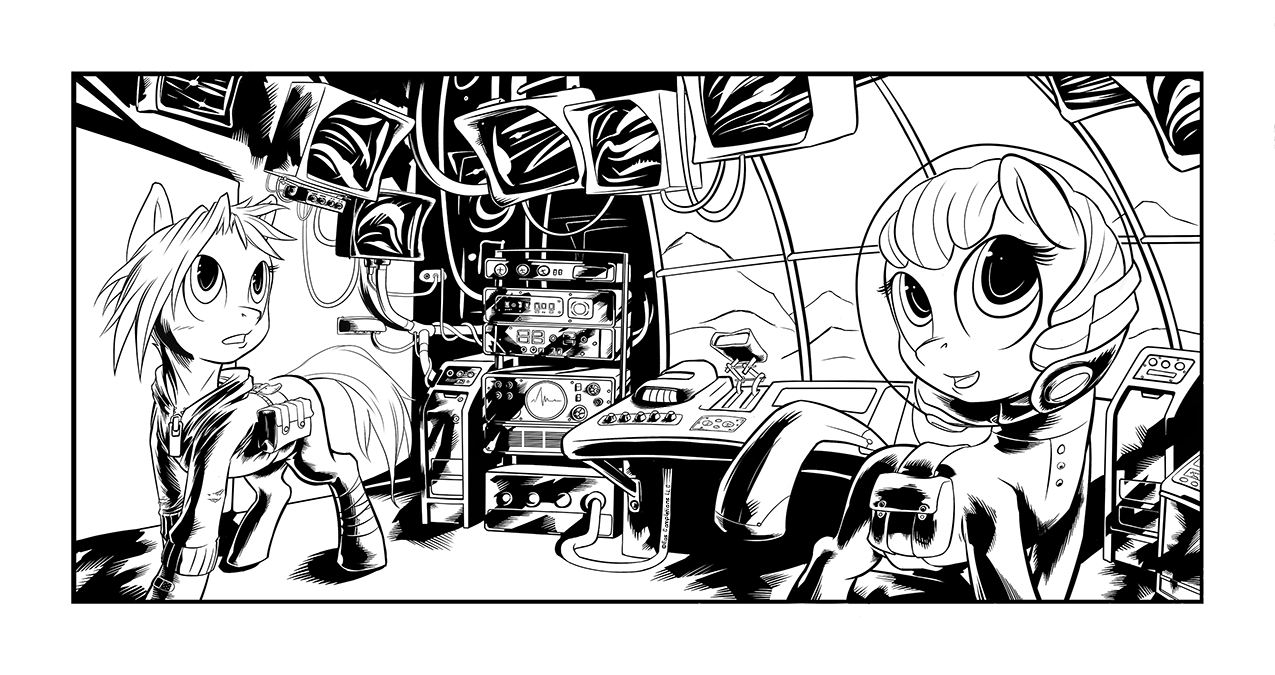
\includegraphics[width=0.9\linewidth]{image08.png}

\begin{intro}
The darkness and the shadows they would always make me fro-own!
\end{intro}


\englishdaytimeplace{7}{3:00 A.M.}{Solaris Tunnel, Tunnel Town}

Trigger Happy yawned and looked down at Puppy, who was playing peacefully on the command room floor. She was moving a toy cart around while making noises with her mouth. She put a couple of bottlecaps on the cart and placed it next to an empty bottle of sparkle cola, then dumped the bottlecaps on the ground and replaced them with the bottle.

``I can has super special minty flavor? 'Kay thanks, bye.'' She was playing quietly, as if she was worried about disturbing somepony by making too much noise.

\thpr{How can she be like that? Just ignore all the horrible things she's seen, and simply sit down and play, like a common foal?} ``Hey, little one, how is your friend doing?''

Puppysmiles didn't look away from her toys as she answered. ``Dunno. She told me it might take a long time, but I have to wait here or it won't work.'' Now she was building some sort of fence all around the empty bottle using\dots

Trigger raised an eyebrow. ``Say, why are you carrying \SI{9}{mm} bullets with you?''

``Oh, these ones? They're pretty and shiny. And it seems that they are needed to use the nine mail mint argon.'' Again, Puppy didn't even raise her eyes.

``The what now?''

Puppy waved a hoof and said in a loud voice, ``Noisy thing.'' A badly damaged \SI{9}{mm} semiautomatic pistol floated up to her hoof, making Trigger step back and take cover behind a terminal.

``Hey, who gave you that? It's dangerous!''

``Nah, it's just noisy. I don't like it very much, it seems more like a colt toy to me. Maybe if it was pink\dots''

Trigger smiled nervously. ``Yeah, Puppy, it's not a very fun toy. Wanna exchange it for something better?''

This gained Puppy's unconditional attention. Her gleaming pink eyes burned into Trigger with expectation. ``Sure, what have you got?''

``Uh, what about a cool pair of sunglasses?''

``Yay! Sunglasses! No wait.'' Puppy frowned. ``I can't use glasses with this stoopid helmet.''

Trigger facehoofed. ``Right. Sorry little one, what was I thinking?'' She went back to digging around inside her saddlebags. ``What about an almost complete \emph{Bridle Gossips} magazine? It's full of pictures of pretty ponies, and there are Fluttershy photos too.''

Puppy trotted to Trigger, took the magazine, looked at it for a moment and smiled. ``I like this one, it's full of pretty ponies! Look at this one. I know her, she's Pinkie Pie! And this one is Rarity and---oh, look here! There's Rainbow Dash too! I lovelovelove Rainbow Dash! She's smart and super cool and she can make the sky go boom! When I'm big I will marry her! I like the picture book, gimme gimme gimme!''

Trigger tried to suppress a chuckle. ``I think we can talk about that, but you have to give me the bullets too.''

``Uh, okie dokie! And what can you give me for the big ones?'' asked Puppy, retrieving a couple of 8.8 Flack AP shells from her inventory.

The mare sighed. This was going to be complicated.

\horizonline

\englishdaytimeplace{7}{3:00 A.M.}{Sugartop Cafe, Tunnel Town}

Sugartop Café was dark and full of smoke, as it usually was late at night. The place was largely deserted except for a couple of drunk ponies nursing the dregs of their bottles, a griffon keeping to himself in one corner, and a pony with a guitar who was largely hidden beneath a sombrero. The bartender was already ``cleaning'' the floor with a bucket of dirty water and a mop that had seen better days, but Jammed Gun couldn't care less.

``Another!'' He said weakly as he raised his empty glass, rattling the blue straw sticking out of it. It remained empty. ``Hey, son of a mule, I said another!'' Waving the glass faster didn't do the trick either. This was upsetting.

The bartender, a silvery stallion with a black mane, trotted to Jammed's table and put down a Sparkle-Cola. ``Hey, big bro', keep it down please. I've got clients sleeping upstairs.''

``Shut the fuck up, Blackie,'' muttered Jammed, ``and fill the glass with something strong. I can't believe she dumped me!''

Black Hat sighed and pushed the Sparkle-Cola against Jammed's muzzle. ``Oh please, Jamie! Forget her already and go to bed. Look, you can use my place upstairs, okay? Just stop drinking. It's not helping you at all.''

Jammed tried to look at his brother's face, but his head didn't want to move from the table. ``You know the bar is half mine, right Blackie?''

``Yes, but you only come in here to mope about your life while I have to deal with the customers and keep it clear of the noisy whiners who drive away the few ponies that actually pay for their drinks!'' Black Hat stomped a hoof on the table. ``Honestly Jamie, you can be a royal pain sometimes.''

Jammed Gun waved a hoof, trying to shoo his brother like an annoying fly. ``Fuck off, Blackie. I feel like manure and I don't want you around. I want booze.''

``I think that instead you should take a trot 'round the town, Jamie. Staying here won't make you feel better.''

``Shut up and give me another wild pegasus, Blackie.'' Jammed raised the empty glass again, keeping his face on the table. ``How could she?''

At last Black Hat snapped. ``Oh, c'mon, Jamie, let's get real! It's Happy we're talking about, the bitchiest mare I've ever kno---'' \emph{SMACK!}

Jammed Gun rubbed his right hoof as he looked down at the prone form of his brother laid out on the bar's floor. ``You know what, Blackie? You were wrong. Staying here made me feel better. Actually, a lot better.'' He trotted outside. ``Thanks a lot, lil' bro!''


\horizonline

\englishdaytimeplace{7}{3:15 A.M.}{Solaris Tunnel, Tunnel Town}

``Say Puppy, how was Equestria two hund---ah, before you left Canterlot?''

Puppy frowned, trying to find a decent answer to the question. ``Greener.''

``Oh, greener.''

``Yup. Mommy was some sort of soldier, but she didn't actually go to war. She was good at fixing things, so she took me with her sometimes, since it wasn't dangerous. I've seen a lot of mighty fine places: a peggysus flying field, a big place underground she called a stable, but it didn't seem like a real stable at all. And I've been in Ponyville, and in a lot of other places.'' She stopped for a moment, pondering what she just said. ``They must be somewhere else, because this 'Big 52' everypony is talking about is not that great, after all. There are no green hills, nor nice houses or pretty places full of happy ponies.''

Trigger felt a knot in her throat. ``You---you don't have to talk about that if you don't want.''

Puppy stared at her, a bit stumped. ``Why not? It's just that this place is not as nice as a lot of other towns I know. Maybe when I find Mom I'll show you those pretty places! Really, I don't know why you insist staying here with a bazillion better places to live.''

``Uh, sure, why not? But, in the meantime, can you please tell me something about Ponyville?''

``Sure! It's the nicest, sweetest, colorfulest town I've ever seen! It was where Pinkie Pie lived before coming to Canterlot! Mommy had to do some work for some pretty ponies and we lived there for a whole summer! It was full of friends and there were trees and hills and super duper colorful houses and a place called Carousel Boutique! But it wasn't a real carousel, it was just a name.'' Puppy frowned. ``I'm telling this because when I asked why the carousel wasn't actually running in circles everypony laughed and Mom hugged me and she was happy, but I felt a little stoopid, so, uh, don't ask why it doesn't move, 'kay?''

Happy giggled a moment and nodded. ``Don't worry, I won't.''

``And then there was this big digging in the middle of the largest apple farm I've ever seen, and there was a house in a cloud that was like a castle, but with rainbow waterfalls! And, and a shop that sold quills and sofas!'' Puppy paused for a moment, studying Trigger's expression. ``Ah, did I say something wrong? Why are you crying?''

``I-I'm not crying, it's just a thing in my eye---''

``Helloooooo fillies and gentlecolts! P7 is here!'' Suddenly all the screens in the room turned pink, every one of them showing a logo of seven balloons tied together.

``Oh, hi Miss Voice! Thank you for coming!'' Puppy waved a hoof at the largest terminal where the balloons had been replaced by a sequence of command lines that chased each other across the screen.

``Thank you for finding me a new home, Puppy! This is waaay better than that stupid Dome where everything was falling apart! Let's see, what do we have here. Oh, geothermal plants, maintenance robots offline, I can fix that. Look at this! A lot of classified data aaaand\dots security alert red? How did I miss that in the first place?'' The voice paused for a moment.

``Is something wrong, Miss Voice?''

``Nah, I need the authorization from a big wig at Solaris Inc. to suspend the alert, but somepony already opened a backdoor in the program and I can just exploit that. It'll only take a moment.''

Trigger was a little surprised. She never liked robots very much, but this one seemed friendly and Puppy knew it, so she decided to wait and see what would happen.

On the other side, Puppy seemed completely at ease. She sat in front of the big screen with her usual naïve faith that everything around her was going to be all right. ``Okie dokie, now can you see if my mom is somewhere in this place, Puppy please?''

% CHECK: naïve ???

``Red alert terminated, all systems green, security doors opening in five, four---Oh, I don't know Puppy, this maneframe has a huge database, and I can't check all the entries because I don't have the authorization. No wait, scratch that! Right here I found some protected files dated three weeks after day zero, but I need a pass code to open them.''

Puppy raised a hoof. ``I know this one! Puppysmiles!''

Happy sighed. ``Now Puppy, your name can't open everything, you kno---''

``Pass code accepted. There are two entries, I'm displaying them on the big screen right now,'' P7 interrupted.

Puppy looked at the writing and frowned as she tried to read it, but it was simply too long for her this time. ``Ah, I can has a little help?''

Happy sat at Puppy's side and put a hoof around her neck in a warm, tender embrace. ``Sure little one. I'll read them for you, all right?''

\medskip

\begin{center}
	\textbf{Day 18}
\end{center}

\wrpr{If I still have the right to pray Celestia, I hope that those eggheads at Stable Tech did a better job than these}---

\medskip

Uh, mules, yes Puppy, it says mules---

\medskip

\wrpr{at Solaris Inc. They succeeded in designing an emergency protocol that transferred all the priorities to the technical staff, but forgot to program the sentinels so that they didn't kill everypony else on the spot.}---

\medskip

uh, this word doesn't mean anything Puppy, let's move on---

\medskip

\wrpr{Anyhow, the tunnel is now safe, so I'll camp here waiting for my crew for a couple of days and loot anything useful for the desert crossing.}

\wrpr{It's almost two A.M. and I can't sleep. I miss her so much. I know she's safe inside the Stable, but I can still hear her calling me because she's scared of the dark or because of a nightmare, then I wake up and realize it's just a dream.}---

\medskip

Fudge\dots yup, fudge---

\medskip

\wrpr{I have to keep busy or I'll lose my mind. I hate Equestria}---

Ah, this part is just a little prayer to the Goddesses---.

\medskip

\begin{flushright}
	\textbf{Rainy Days.}
\end{flushright}

\medskip

Trigger sighed. \thpr{When Mrs. Rainy Days wrote this entry she hadn't her daughter in mind as a reader.} ``Well, it seems that she headed south after all. Let's see if the other record has something more.''

P7's voice interrupted the two ponies. ``Hey Puppy, do you remember the pass for Chief Sand Box, pretty please?''

Puppy tapped her helmet for a moment, thinking about it. ``Magenta? No, wait, Agatha!''

% ``Thanks a lot sweetie! I'd hug you super much, but under the circumstances---Uh, let's do this! Hug yourself and pretend it's me! Here's your second entry! I'll be away for a little, poking my nose where I shouldn't. Have fun and don't mess around!''

``Thanks a lot sweetie! I'd hug you super much, but under the circum-\\stances---Uh, let's do this! Hug yourself and pretend it's me! Here's your second entry! I'll be away for a little, poking my nose where I shouldn't. Have fun and don't mess around!''

% NOTE: force to break line

\medskip

\begin{center}
	\textbf{Day 21}
\end{center}

\wrpr{I'm finally ready to move. Apparently nopony is coming in this direction, so maybe I'm the only survivor in the area? Not sure, but I don't want to test my luck. I'll take a detour to avoid Sun City. The place was badly hit, and last night I could see a discouraging glow in the desert, exactly where the city should be. If I'm lucky, in a couple of days I'll be at Blue Feathers Airfield. I'm moving out at first light.}

\wrpr{I'm back, I couldn't sleep again. Another nightmare. I can't stop dreaming of Puppy lying dead in the kitchen.}---

\medskip

Fudge, Puppy, fudge\dots Do you like fudge? Okay okay, I'm reading!---

\medskip

\wrpr{these dreams. She is safe, I'm sure of it. She would never disobey me. Why do I keep dreaming of her? I found some pills, and I think that some of them could help me sleep. If this nightmare returns, I'll begin taking them.}

\medskip

\begin{flushright}
	\textbf{Rainy Days.}
\end{flushright}

\medskip

Puppy was hugging Trigger, pressing her helmeted muzzle into her back. ``What's wrong, little one? She just misses you, but you are all right. When you find her, she'll see that you're safe and there will be no bad dreams anymore, all right?''

Telling such a shameless lie physically hurt Happy's heart, but Puppy needed all the encouragement she could get right now.

``I-I'm not a good pony, Miss Happy. I didn't went to the secret place because I wanted to see the fireworks!'' She bawled loudly. ``I'm a bad pony! Mom will be mad at me!''

Trigger returned Puppy's hug, trying to reassure her. ``Now, now, don't worry. Your mom said that she was going south, right? To a place named, ah, Blue Feather something---I think it's what we call Rust Manor. It's easy to get there! It's just past Sun City. I'm sure that she will be very happy to see you.'' \thpr{Why am I giving hope to this poor creature? Her mother is long dead, what am I doing?}

Puppy looked at Trigger with those two large, gleaming pink eyes now filled with new hope. ``Really? Will she be there?''

``I-I don't know if she's still there, but you want to follow her steps, right? If you want to find out what happened to her then you have to follow the trail as long as it is still fresh!'' \thpr{Yes Happy, two hundred years fresh.}

She smiled again. ``Right! I arrived here with no problems at all, so I can follow Mom anywhere! Thank you, Miss Happy! You are the best pony!''

P7 interrupted them once again. ``Very well, I'm done with the inventory. Those guys at Solaris had quite a good grasp of the whole 'end of Equestria' concept. This place is full of labs and storage silos with enough firepower to give the survivors a second show! Oh, and Puppy, I think you were trying to say Pinkie Pie.''

Puppy raised her head. ``Wut?''

``Oh, it's quite simple my little friend. Under the mountain there are levels and levels of warehouses filled with military equipment ready for use. There is enough firepower to kill every inhabitant of Equestria at least twice.''

``Ah, and by kill you mean hurt very much?'' Puppy asked doubtfully.

``Nopey mopey. I mean hurt way too much! Something like a party so big that nopony will be here to tell the story the day after.''

``A Pinkbot party?'' asked Puppy, now afraid of the answer she could receive.

``Pinkbot: file not found.''

Puppy stopped a moment to think. ``Okie dokie, what these things do exactly?''

``Let's give some examples. Multi-plasma long range warhead. This baby can hit fifty-six different targets with high penetration, self-propelled independent micro-missiles. Every missile can easily pierce the wall of a bunker and fill the inside with plasma, raising the temperature by a couple hundred degrees, killing everypony within. The Multiport Disruption Generator dismembers every living target in a range of one hundred meters. Obviously this kills ponies. Chocolate chaos is a magic energy gun that converts the blood of the target into chocolate milk. The effect is reversible, and the blood returns to its original state after half an hour, but the victim dies almost instantly after being hit.''

Puppy interrupted the list. ``Okay, okay, I got the picture!''

``Very well, what do we do then? You're the boss here.''

At the computer's last statement, Trigger raised a hoof to try and stop Puppy from saying anything stupid, but Trigger wasn't fast enough.

``Dump it. Make a hole and dump everything inside, build a house on the hole and then move all the bullybots you have inside the house so that nopony can never ever get hurt.''

``Well, technically everything is already in a big hole under a mountain. I can detonate the elevator shafts and the tunnels between the storage areas so that they'd be sealed forever unless somepony digs the whole mountain away.''

``Do it!''

Happy gave a long sigh of relief.


\horizonline

\englishdaytimeplace{7}{3:30 A.M.}{Tunnel Town, Big 52 N Branch}

Jammed Gun hit the metal door of the Tunnel with his head, again.

``Fuck, I knew I had to stop her. Fuck, fuck, FUCK!''

``You know, Jamie, the door won't magically open just because you bucked it.`` Black Hat sat at his brother's side, still rubbing his right eye. ``I guess I deserved it, somehow. This doesn't mean I won't give it back someday.''

``Oh for Luna's sake, Blackie! Put a steak on that eye and go to bed so that I can mope in peace!''

Black Hat leaned against the wall and yawned. ``No can do. Can't leave big bro' like this. Besides, I'm gonna be laughing at you for months over this.''

Jammed Gun snorted. ``I always suspected that our mother was a bitch, but now I'm sure of it. Happy is gone and you think about laughing! Do you want another black eye, or this time are you trotting away on your hooves?''

``Hey cool down, geez! There's nothing you can do anyway while these babies stay cloOOH!''

With a metal clank the large doors started lifting, sending Black Hat sitting on his haunches. ``What the fuck?'' he shouted.

The two ponies stared in disbelief at the gigantic metal bulkhead, a monster more than a meter thick, rising into the tunnel's ceiling. As soon as the first door was completely opened, a second pair of doors retreated into the tunnel's sides.

It took almost half a minute before Jammed was able to speak again. ``Is-is this for real? Gimme a pinch.'' \emph{SMACK!} ``You son of a ghoul, I said a pinch!''

Blackie snickered. ``I told you I owed you one, and you said she was dead for sure!''

They stepped into the tunnel, ignoring the skeletons beneath them. Black Hat went to a cart peppered with bullet holes, rummaging through its contents. ``Woah, look at all this stuff! Guess what? This town is getting its share at last!''

Jamie trotted a little farther, watching as the lights of the tunnel began to turn on and illuminate the immense length of the six kilometer underground passage. A rope was dangling from an opened ventilation grate in the ceiling. His trot became a gallop and he rushed deeper into the mountain.

``Hey, big bro! Don't rush like that! We should call the other guards!''

``Fuck the guards! I'm drunk \emph{and} in love!'' his voice echoed off the tunnel's walls.

Black Hat sighed and galloped after his brother. ``At least wait for me!''


\horizonline

\englishdaytimeplace{7}{9:00 A.M.}{Trade Station Tunnel South, Big 52 SC Branch}

Trigger hugged Puppy and kissed her on the helmet. She tried to break free with an annoyed expression. ``Yeuch, smooches! Not in front of everypony!''

All the town guards and many other dwellers of Tunnel Town surrounded them. A mare that acted as the local authority gave a little speech and a pouch of caps to Puppy before Trigger Happy accompanied her out the south end of the Tunnel.

In front of the two ponies lay an endless landscape of sand dunes, disrupted here and there by some red, rocky formations. In the distance it was possible to spot the blurry silhouette of a city, but the sand in the wind made it almost impossible to tell if it was actually a town or some sort of natural formation.

``Very well, Puppy, we're here. That's Serpent Desert. Now let me explain how to get to Rust Manor. Are you listening?''

Puppy smiled and jumped in the air. ``Sure, Missus Pretty Happy!''

``Very well, the desert is the Sand Sweepers' territory. They're mostly scavengers that move a lot among the various camps, salvaging anything useful they find under the dunes. Usually I'd warn you against them because they tend to do some robbery here and there, especially on lone travelers, but I don't think that they'll try to rob you, since the Sweepers are quite the superstitious tribe and probably know about you from Lonesome Pony.''

Puppy nodded. ``Pretty ponies that walk around a lot, okie dokie.''

Trigger smiled. ``There is a trail to follow. It's quite easy to see because every fifty meters the sweepers planted a red banner. You just trot from one banner to the next and you'll be at their first encampment before tomorrow morning.''

Puppy frowned and pointed at the more inviting highway built on a solid bank and running straight south. ``Why can't I use that? With my scooter I'll be there lickety split!''

``No, little one, that highway leads directly into the middle of Sun City. You must avoid Sun City at all costs.''

``Why?''

``It's a dangerous place. Everypony that goes there doesn't come back, and nopony knows why!'' Trigger's tone brooked no argument, but Puppy was not the most astute of audiences.

Puppysmiles tapped her helmet as if it was her chin. ``Uh, maybe they like it so much that they don't want to go away?''

``I-I don't think so, Puppy. When I was a foal like you, Sun City was the home of a tribe: the Rust Scrapers. They were allied with the Sand Sweepers a long time ago. Anyhow, at some point it was said that the Sweepers found something big, but the Scrapers stole it from them. There was a big fight, something like a betrayal because the Sweepers tried to take the City with a night assault.'' She paused to see if Puppy was still paying attention.

``And then what happened?'' she asked with a worried expression.

``During the assault something went completely wrong, but nopony knows what. The only thing we know is that the Sweepers went in with every gun they had and never came back. Everypony who tried to investigate the city disappeared, apparently devoured by its secret. the Sweepers that didn't participate in the fight, mostly foals and the elders, put together what was left of their tribe and carried on, trying to survive.''

``Oh, so they were all bad ponies?''

Trigger frowned. ``In the Wasteland it's not always easy to tell good from evil, Puppy. If you want to survive, sometimes you have to leave something behind. Make sacrifices. Dying a little bit instead of dying completely.''

``Wut?'' She gave Happy a puzzled look, unable to understand such a deep concept.

``Don't fret your head, little one. Just think of it as, well, yes, they were bad ponies, but they couldn't help it.''

Puppy shook her head. ``That's not true! If you are mean to somepony you are mean and that's all! No excuses. If you begin to think that you can be just a little mean then you'll end being super duper mean in no time, and you'll be a bad pony too!''

``This\dots did you think of this on your own?'' Happy stared at Puppy in admiration.

``Nopey mopey. Mom told me!''

Trigger patted Puppy on the helmet, seeing her worried face. ``Don't worry, robots don't count. Mommy won't be upset. C'mon, show me a pretty smile.''

Puppy smiled and jumped on her scooter. ``When I find Mom I'll tell her that you've been nice to me! Thank you very much, pretty pony Happy!'' She launched herself down the road, gaining speed as she descended toward the desert. ``WEEee!''

Trigger watched Puppy grow smaller as she scooted off into the distance. ``I'm so sorry, little one.''

``So, Happy, ghost or foal?'' Jammed Gun trotted to her flank, smiling.

``I still don't know.'' She sighed. ``The only thing I know is that she's lost.'' Happy turned to look at him and smiled a little. ``And what about the black eye?''

``Brotherly love,'' Jammed stated, before immediately getting back on topic, ``and who isn't lost in this cursed world? As soon as the news spreads, ponies will head for Tunnel Town. We need more guards.''

``Speaking of that\dots The goods in the carts need to be recovered, stockpiled, and divided equally between everypony. Keep an eye on Black Hat.''

He nodded, sighing. ``Yeah, don't worry. The others are already taking the carts into town. A couple of them are branded. There's a caravan of three carts from the Water Herders and a cart that belonged to the Gallopers, but it was salvaged by the ponies when they tried defending themselves from the sentries. Are we giving 'em back?''

``We should, at least as an act of good will. If we show them that their goods were preserved maybe this will help us later. Oh, and remind me to teach you how to restart the tunnel in case it shuts down again.''

Jamie hesitated for a while. ``Well, uh, about last night. You know, when you ran after the gho---ah, Puppysmiles, and I wanted you to stay, uh\dots Can we pretend that I said nothing about, well, you-know-what?''

Trigger Happy giggled. ``I don't think so, Casanova. That was the clumsiest confession ever, and I'm totally going to haunt you about it for the rest of your life.''

Jammed groaned, lowering his head. ``Aw, why did I even bother asking?''

``May I ask you something now?''

He waved a hoof. ``Yeah, sure, go on. Shoot me in the heart.''

``Am I still in time to say that I love you too?''


\horizonline

\englishdaytimeplace{7}{4:00 P.M.}{Serpent Desert, Big 52 SC Branch}

\rtpr{Good afternoon fillies and gentlecolts! This is Lonesome Pony, and you're listening to Radio 52! The only and best radio in this slice of Equestria! Yesterday, I was walking in the street and a mare asked me, ``L.P. how can you be so good on your program? Everypony here listens to you\dots'' Well, I must admit that it's not easy, but luckily enough I'm the only fucking DJ around!}

A weak ``\rtpr{yay}'' from a feminine voice interrupted the monologue.

\rtpr{Bad L.P., you used the 'F' word. You can't use it! Not with our heroine listening to you! Right, right, I'm a bad pony and I should feel bad. Instead right now I feel just great, because guess why? You can't? Obviously not, because I'm the first one with this treat on the table. Fresh from the wings of a friend of mine coming from the south! Hold your reins, little ponies, because this is BIG!}

At that point the radio delivered a static charge and went mute for several seconds, but the static was soon replaced by the voice of Lonesome Pony laughing.

\rtpr{Ah, I had you all! You fell for it! Nopony can shut up Radio 52, and especially not today, because today we are celebrating THE TUNNEL REOPENING! Yes my little ponies, your ears are working! Tunnel Town is back in business! No more mountain pass and landslides!}

Boisterous, triumphant music played for almost a minute with the DJ making guitar noises with his mouth in the background.

\rtpr{Best thing since the destruction of the Carnival, and guess who did this? Oh yes, our guardian angel, our little yellow ghost! We needed a foal to save us all from a horrible death by starvation? Bucks, now I'm depressed. No, seriously. In a week this little devil has saved three towns from their worst nightmares. A FOAL! C'mon 52, raise your head and show some guts! Till then, I'll be here worshiping a way-too-few-years-old pony.}

There was a silent pause before the voice of the DJ came back, tired and old.

\rtpr{Wake up, everyone out there. She is just one pony. She can't save us all. We have to save ourselves with what we've got. We need only to be better ourselves. We don't need another hero.}

An acoustic guitar started playing while another song began, but this time it wasn't a record. The singer was Lonesome Pony himself.

\begin{music}
		Out of the ruins, out from the wreckage
	
		Can't make the same mistake this time.
	
		We are the children, last generation.
	
		We are the ones they left behind\dots
	
		And I wonder when we are ever gonna change it,
	
		Living under the fear till nothing else remains.
	
		We don't need another hero\dots
\end{music}

\horizonline


``Wow, I really hope I find this super filly hero they always talk about! Do you think she'll want to be my friend?'' Puppy was trotting on the sand, following the red banners just like Trigger Happy had told her to.

{\mt ``Affirmative. Usually a heroic figure is prone to be friendly. Warning. Mild radiation detected. Threat level: negligible.''}

She trotted for a while before hesitantly asking, ``Ah, Mister Voice, do you think I'm good? Will my mom still love me?''

{\mt ``Warning. This program is not designed for behavior evaluation.''}

Puppy sighed with frustration. ``Geez, you always hide from every important question, don't you?'' She was going to add something, but her attention was caught by a figure standing on a dune not far from the trail. ``Hey look, a pretty pony!''

The ``pretty'' pony consisted of an old unicorn with a white mane and a red coat, dressed in a mantle that covered her almost completely. Strapped across her back was a long lever action carbine. As she approached, the mare simply smiled. ``You took your time, little ghost. I've been waiting for you since noon.''

``Hi! I'm Puppysmiles!'' She smiled and waved a hoof. ``I'm sorry I'm late\dots Uh, late for what?''

The slightest of smiles ran across the old mare's face before she replied. ``Well, for adventure of course, little one. Do you like adventure?''

``Yush! I lovelovelove adventure! Where is it? I can has two?'' Suddenly, her enthusiasm came to a halt. ``No wait! I have to find Mom, I really shouldn't go adventuring\dots''

The old mare chuckled. ``Oh, right, you are already following a path, how could I have forgotten?''

Puppy nodded. ``Exactly! So I'm sorry, but I've got to go. 'Kay thanks bye bye!''

``And if I say to you that this adventure is about a friend of yours being in danger?''

Puppy was already trotting away, but the mare's last words made her turn on her tail. ``A friend of mine in danger? Who? Why? Where? When?''

``Now, now, don't rush like thi---'' Puppy jumped at the elder's neck, pressing her helmet against her muzzle and staring straight into the eyes of the unicorn.

``Please please please tell me! Pleeeeease!''

The mare staggered, almost losing balance. ``Calm down, little ghost, I was telling you! Just sit down and listen, all right? Behave and I'll tell you everything!''

``Uh, yeah, right\dots Sorry, miss pretty old pony.'' Puppy let go of her neck and sat in front of the unicorn, who sighed in relief.

``Very well. I'm Long Ears and I'm a farseer, a unicorn that can see distant places and ponies.''

Puppy jumped up onto her hooves. ``Uh! Can you see my mom? Can she see us? Is she okay?''

``It doesn't work like that.'' Puppy deflated, sitting down again as Long Ears continued, ``I take some medicine, and in my dreams I have visions, but I can't chose what I see. Last night I had one of those dreams, and it was about you.''

Puppy sat down in silence, listening intently to Long Ears.

``You asked a very special friend a very important favor. Your friend did her best, but a really bad turn of events made it impossible for her to accomplish her task, so she appeared to me in my dreams and I knew that you were coming here.''

Puppy frowned. A friend she asked a big big favor from? She didn't ask for---\thpr{here, Silky Tail. Look after Henrietta and don't let anything bad happen to her.} ``Henri? She is in danger? Where?''

Long Ears nodded and pointed a hoof toward the distant silhouette of Sun City. ``I'm afraid that the eagle flew too near to the sun, and she can't find a way to come back.''

Puppy hesitated. ``But-but Happy told me that I can't go there! I don't want to disobey her!''

Long Ears shrugged. ``You don't have to. You asked a friend for a favor and she wanted me to warn you, that's all. You could simply chose to ignore her and go on your way. One way or the other, my task is over.''

``B-but something bad happened to Henri! I can't leave her alone, she could be hurt! She\dots she could be crying!''

``Well then, go to Sun City and save her. But I must warn you, Sun City is a trap. A bad dream made real. Once you start dreaming, you will never be able to leave.''

``Oh don't worry, I'm not sleepy at all!'' Puppy smiled as if it was an easy thing. ``Space Captain Andromeda to the rescue!'' She galloped away, heading for the town behind the dunes.

Long Ears watched Puppy running away until she was a gray spot in the sand, then took a pill from a pouch and swallowed it together with a gulp of a milky potion. When she blinked she could see flames rising from the town and hear the sound of battle. ``What am I seeing? Past or future?''

A giggle came from the mare's side. ``She's lively, always smiling. I like her! If only more ponies were like that filly instead of being all grumpy faces\dots''

She whispered, ``Can a living nightmare bring peace? I'm not sure of this.''

``Don't ask me! I'm only a vision caused by your massive consumption of hallucinogens! Really, it won't help you very much. Things will happen the same way even if you don't see them coming, and you can't even tell what's coming from what already happened.''

Long Ears sighed. ``Well, maybe you're right. Let's go home.''

``Yeah, let's go. That puppy can fend for herself.''

\clearpage

~\vfill


\begin{engnote}
		Level up! (7)
	
		New perk added: The power of metal - there are moments when rock is not enough. You inflict 5 additional damage with HtH attacks (yeah, rocks and power hooves are considered HtH weapons)
	
		New Quest Perk added: Spirit of 52 - Your legend is growing: you will have less low level random hostile encounters as long as your standing with all the tribes is at least neutral.
\end{engnote}


\chapter{Sun City}

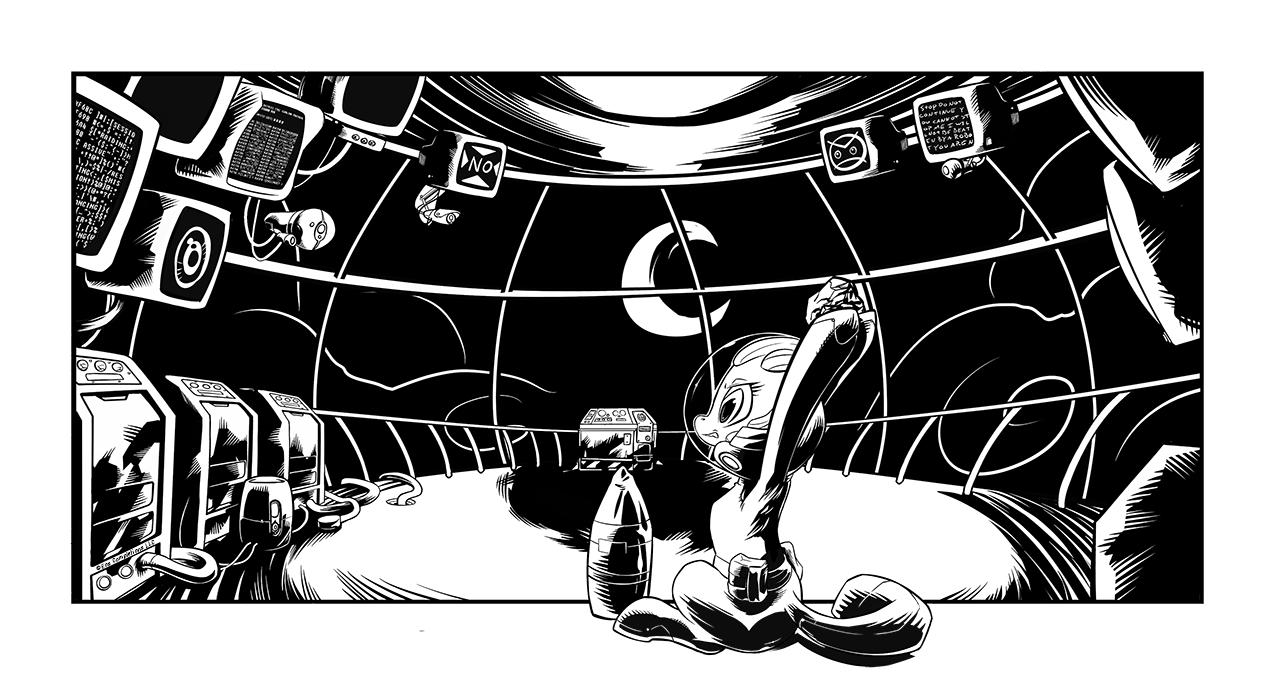
\includegraphics[width=\linewidth]{image09.png}


\begin{intro}
    Sun City is more than a town: it's the remedy to ponykind's derailment.
\end{intro}

\englishdaytimeplace{7}{11:00 P.M.}{Sun City Suburbs, Big 52 SC Branch}

The trip to the city had been quite long and by the time Puppy arrived at the first houses darkness had already descended on the streets. Sun City featured a central group of commercial and administrative buildings surrounded by residential areas. However there were no lights in any window, nor signs of anypony living there. The neighborhood Puppy was trotting through had been almost completely scavenged for construction material, leaving only the skeletons of houses resting in the ever present sand; it was like a desolate boneyard, filled with carcasses that had once been called `home'.

Now, Puppy wasn't eager to admit that she still was a little afraid of the dark, but the whole place was a little too similar to her first day in the apocalypse to let her just shrug it off and keep going. ``Why that chicken had to be in danger in such a scary place? Stoopid Henri, there's nopony here, why they call it a city if it's empty?''

Each step took her deeper into that scary place. Where did the colorful signs go? Puppy never went out very much at night but she was pretty sure that a city didn't work like this\dots She wanted some music to hide the sound of the wind howling through those bony houses, but the radio had gone mute when the filly reached Sun City's outskirts and the unusual silence made her feel lonely. ``Hey, mister Voice, you there?''

A discharge of static was the only answer Puppy got from the suit. ``{\mt Fzzt -cation BbZzzZzT -ched. Elctr- SkrackLE -ference. BzaP! -sible sustaining vo- BzZzT! -terface.}''

``Aw, he's grumpy again\dots'' The filly frowned and kept trotting. The HUD of the helmet started to display written warnings on the screen, but showing fast scrolling technical messages to a foal that couldn't even read without spelling every single letter was a waste of time. This left the filly completely alone: the radio was gone, mister Voice was gone, this was like those times when she tried to sleep but the room was too dark and the wind outside made strange noises. They were the nights when she'd hid under the sheets and called out for her mother until she came and nuzzled her, singing a little lullaby to make her feel safe and warm. Puppy actually tried to sing something, but the only thing she could think of right now was the evil enchantress song and no, it didn't help at all.

The little pony's steps echoed in her head like the beat of drums as Puppy walked through a never ending maze of identical streets, with every empty window reflecting her eerie pink glow. What was that? Maybe mister Horse Tile came back from the grave and was following her? Even mister Horse Tile would have been welcome at this point\dots A distant metallic screech froze the filly in the place; her rump hit the asphalt and she completely stopped moving.

``W-w-whatwasthat!?'' Sure, dealing with bullybots and running after mom was not a frightening thing, having to face ghoulie ponies could be scary but at least you knew what you were fighting\dots but this one was different: an empty town filled with empty houses and crisscrossed by empty roads during a clouded night? And with ghostly sounds too? Why did she think about ghosts now? No ghosts, bad ghosts! Why did she leave the red banner trail? Miss pretty pony Happy told her not to leave the trail, but she had to come and help that stoopid chicken and now it was dark and it was scary and Puppy missed Miss Silky Tail so much!

The filly flattened herself against the road and lowered her ears, trying to make herself disappear. ``N-new plan, we wait here till it's day!''

Another creak echoed in the empty streets, like the suffering wail of a tortured soul.

``EEEEEEK!'' Puppy jumped on all four hooves and started galloping faster than Rainbow Dash at the Running of the Leaves. ``Newest plan! We're out of here till it's day!''

\begin{center}
Sun City 1 -- Puppy 0    
\end{center}

\horizonline

\englishdaytimeplace{8}{8:00 A.M.}{Sun City, Big 52 SC Branch}

During the day, the city was quite similar to the suburbs of Salt Cube City, or even Canterlot; not scary at all, just\dots ugly; Puppy wondered why she had been so scared, what a silly pony she was!

``See, mister Voice? There's nothing to be afraid! It's just another town, with broken houses and broken roads and-'' For a moment Puppy's eyes caught the silhouette of a flying pony, ``and pretty peggysuses! Yay!''

The foal launched herself into a gallop, chasing the flying figure. ``Hey! Hey mistur peggysus wait for me! WAAAAAIT!'' Galloping at top speed while looking into the sky, Puppy wasn't properly watching the road in front of her and collided with another pony in the middle of the street. ``Owie, why don't you look where you're going? I was running here before you!''

The pony was an adult earth stallion with a brown coat and black mane; he had been carrying buckets full of bricks and building materials on his back, but now everything was scattered over the asphalt. Puppy jumped onto her hooves ready to zoom away just in case the older pony was mad at her, but he simply put down the buckets and started filling them again.

``Uh, yeah, you better say nothing\dots and don't stay in the middle of the road again like a dumb statue!'' Puppy stuck out her tongue, but noticed that the earth pony wasn't even paying attention to her. Actually, he seemed a bit\dots well, how to put it\dots

``Ah, sorry mister pony, are you deaf? I'm Puppysmiles and I'm looking for my mom\dots well, usually I do that but today I'm saving my friend Henry that came here and then had some sort of troubles but I still don't know what kind of troubles. Have you seen her? She's a chicken but she doesn't want me to call her that way but I mean, duh, she has a beak and feathers and everything else, she must totally be a chicken. Once I knew a pony that was a zebra, I don't know why ponies don't like zebras, anyhow this zebra didn't want to be called zebra but everypony called her that all the same, so maybe she's just like zebras, maybe ponies don't like chickens here\dots dunno\dots''

Puppy followed behind the earth pony as he, without saying a word, gathered everything that he had dropped and headed toward the center of the city. In the light of day, Puppy could see that past the outer town borders the houses had been completely dismantled, leaving a vast area of flat terrain traversed by an intricate web of paved streets in a ring of at least two hundred meters all around downtown. It seemed like some sort of nopony's land, but it was the result of the methodical demolition of every building that had stood in the area, brick by brick instead of simply flattening the houses. They weren't even using the ruins as defensive positions; the buildings had been salvaged down to their foundations.

Puppy stopped and gazed in wonder at the shining city that lay at the heart of the empty land. ``Wow, you have a pretty town here at last, I like it!''

Right in front of the filly in yellow stood a city of the old times: there were some small houses with painted walls and clean windows, no holes in their roofs nor planks nailed over the doors. Puppysmiles stared at the ponies trotting around and carrying things, it was a lively place: everypony was doing something, even the foals and the pegasi. There were pretty houses and pretty skyscrapers; even if the gardens were a little yellowish there was actual grass in the yards and there were even trees here and there. Puppy wouldn't have given this place more than a six out of ten, but hey, this was the first town along her way that deserved a vote at all!

``Really, Happy was super wrong\dots'' Puppy trotted after the brown pony she had bumped into earlier, ''ponies that arrived here actually liked it so much that they didn't want to leave! I was right as usual, ah, take this miss Happy! Sure you aren't very chatty mister pretty pony\dots'' Nope, not chatty at all, Puppy decided to leave the earth pony and wander by herself so she could check the place out. It was really a nice town and reminded her of some of rhe places she had visited with her mom: after eight days of wasteland being in such a nice place was refreshing, even if these ponies had something wrong with them that Puppy couldn't put her hoof on.

The filly in yellow searched the area for some other pony to talk to, and noticed a griffon crouched on a roof; he was replacing some damaged tiles. ``Hey mister chicken, have you seen my friend Henri? She' a chicken too!'' Nope, no answer at all; in this place everypony had to be deaf or really unfriendly.

Puppy saw a unicorn mare watering a tree, and tried to approach. ``Ah, excuse me miss pretty pony, have you seen a chicken named Henrietta please?'' Nothing again, the filly's frustration was growing; it was quite obvious that she was getting nowhere, this situation needed something better: ``Uh, she's half kitty too.''

The unicorn kept watering the tree despite Puppy's efforts, but this time the filly wasn't going to give up that easily: she put herself physically between the tree and the unicorn, staring her right in the eyes and\dots and\dots DERP! ``Ah, your eyes are\dots uh, weird\dots''

The mare had a walleyed expression and seemed frankly dumb. ``How do you make that trick with the eyes?'' Puppy tried crossing her eyes and almost fell on her rump, ``It's hard! How can you look straight with eyes like that?''

Again, the foal was completely ignored. The mare tried to circle around Puppy a couple of times, but the filly in yellow insisted on staying between the unicorn and her tree; in the end she watered Puppy's head and went away.

Puppy was now wet and upset. ``Hey, that's not very nice! What's up with everypony here? Why don't they want to talk with me, do I stink?'' The filly tried sniffing herself but it was quite pointless since she was sealed inside the suit.

The foal wandered through the neighborhood for half the morning, trying to find somepony who would talk to her, but everywhere it was the same: everypony had the same walleyed expression and didn't listen to her, not even the ghoulies.

She could remember something like this, a movie with a strange title that her mom forbid her to watch, metrodontremember\dots anyhow she tried looking it but it was boring to death. This city was just the same: like a warped reflection of the barns of horrors where fun could actually kill you, here the boredom could turn you to stone.

Her exploration took the filly deeper inside the town and nopony tried to stop her or seemed to acknowledge her passing Even when Puppy approached some foals trying to play with them, they simply kept working; she really did her best to make some friends, proposing some games like pin the tail on the pony and even something exotic, like playing space ponies and the tomato aliens, but nothing. Now she was feeling ignored and a bit sad.

``Mister Voice has gone away, Henri is nowhere to be seen and all the pretty ponies play dumb and don't want to talk with me. This is the worst city ever! Who cares about the pretty houses or the nice trees if there is no fun at all in first place? Why is everypony acting this weird?'' Puppy sighed; she knew for a fact that in each town there was at least a mayor or something like that, maybe she could find some answer if she asked that pony. Usually important ponies lived in the middle of town and this was quite good, because finding the center of Sun City was easy even for a silly pony: those giant skyscrapers were quite hard to miss.

The little foal trotted past the residential area and arrived in a wonderful and well kept block of tall buildings, with glass walls and picturesque statues of Celestia and Luna. Around the marble princesses were fountains that spilled clean water, and a big metal tower stood right in the middle of everything, like a focal point for the whole city. Puppy lifted her head as she looked around at the various buildings: there were half a dozen towers of various heights, but one of them stood out because of it's shiny metallic structure; it was like a spiral growing into the sky for about twenty stories and then abruptly ending in a large platform, like an overgrown mushroom.

``This one seems easy!'' Puppy trotted toward the tower only to find herself being lifted off the ground and floated away from her destination. ``Wut?'' The foal tried to twist around and saw that an adult pony had picked her up by the back of her neck and was taking her away toward the residential area.

``Hey! Lemme go! Meany pony I wanna go to the shiny tower! I gotta see the mayor! It's important, you dumb walleyed pony, are you listening to me?'' The pony put Puppy down just outside of the city's borders in nopony's land, leaving the protesting foal still yelling at him.


\begin{center}
    Sun City 2 -- Puppy 0
\end{center}

\horizonline

\englishdaytimeplace{8}{2:00 P.M.}{Sun City, Big 52 SC Branch}

Puppy spied on the working ponies with a resolute look on her face: they didn't want her in town and wouldn't tell her why, but she had to get inside somehow\dots maybe she needed to play smart, with some sort of disguise using a sombrero and a poncho and maybe an accordion\dots yeah, that could actually work, but where to find fake mustache at this hour?

Suddenly, the filly was distracted by another flying figure in the sky. She had grown used to pegasi flying to and fro around the outer part of the city, but this one was different: it was a griffon, a little griffon with familiar armor\dots ``Henry! Hey Henri, wait!'' Nope, even her best of bestest friends wasn't listening to her now; Puppy would have felt disheartened if she wasn't busy finding a way to get Henrietta's attention, ``Rock!''

\emph{The Rock Of Destiny} floated to Puppy's hoof, she took a moment to aim aaand\dots ``Bull's eye!'' The griffon unleashed a panicked screech as she dropped out of the sky like, well, the rock that hit her.

``Don't worry I'm catching you Henri!'' Puppy threw herself into a gallop, trying to catch her feathered friend before she hit the ground. In the meantime Henrietta struggled desperately to regain control, but she was still stunned: all she could do was to try and aim for something soft\dots but what? A yellow spot appeared in her peripheral vision. A yellow spot that was yelling and moving fast.

``I got you I got you I got-''

THUMP! ``Owie!'' ``Yeow!''

The young griffon blinked, looking at Puppysmiles. ``What the fuck are you doing here, Puppy? This place is dangerous, run! There's a strange buzz tha-'' Henrietta derped and immediately stopped talking; a trickle of blood from her head injury ran down her beak but she didn't even seem to notice.

``Henry I found you at last! Silky Tail told me that you were in danger and- HEY! Where do you think you're going!?'' The griffon opened her wings, getting ready to take-off, but the filly wrapped her hooves around Henry's neck and held on tightly. ``Don't even think of going away! Now we are getting out of this stoopid place and you are coming with meeEEEH!''

Henrietta was bigger and stronger than Puppy, and she seemingly felt no remorse in using brute force to push her away before taking to the air once again; the filly rolled head-over-heels a couple of times before finding herself sitting in a pile of rubble in nopony's land, alone once again.

``What the\dots what happened to her all of a sudden? The other day she was all let's work together and then she was wounded and I helped her and now she just scolds me and flies away\dots this is not fair, not fair at all! Very well, if she doesn't want to be my friend, then I want Silky Tail back!'' Puppy galloped back into town, looking for her ex-friend, but almost immediately came to a stop and reconsidered her last thought, ``But I gave her Silky as a present, I can't take a present back\dots but I want back my friends, at least one of them.''

Puppy shook her head. ``No, I want both of them back! I'm not going away without Henri AND Silky Tail! I only need a better plan!'' But what plan? During the day the ponies were all around the place and didn't let her walk into town and during the night the city was so scary\dots or maybe not? After all, this wasn't a ghost city\dots

The foal went back to sitting just outside of the town borders and looking at the not-really pretty ponies working endlessly and mindlessly. She had come up with a masterful plan\dots now she just had to recover The Rock Of Destiny and wait for night\dots Half hidden behind a pile of rubble, Puppy lurked, ready for the decisive strike. ``Soon\dots''


\begin{center}
    Sun City 3 -- Puppy 0
\end{center}

\horizonline

\englishdaytimeplace{8}{9:00 P.M.}{Sun City Downtown, Big 52 SC Branch}

The little filly crept through the dark, crawling with her belly on the ground and her ears flattened. ``Sneaky sneaky\dots'' She uttered a couple of whispered words, nothing more: like those oriental ponies who did all that cool stuff she was told about but she had never actually seen because mom said they were violent\dots sometimes mom was a pain. But none of that mattered because now Puppy was a filly on a mission, and she had to focus and be super sneaky and move like a shadow in the night!

Wearing a yellow suit and a pink glowing fishbowl. ``Sneaky sneaky\dots''

The plan was easy: go past the enemy lines, find the boss of the place, tell him his town stinks then go find Henri and run away in the sunset, like in that super cool movie with Pone Wayne. Now, first things first: poke her nose into the super pretty place with the skyscrapers and have at least one ride on the elevator. Okay let's get real: ride the elevator until it melts.

The city was completely empty during the night: everypony was somewhere else, probably sleeping, but this time Puppy knew that there were no ghosts in this place, only grumpy faces. Reaching downtown had been an easy task and nopony blocked her when she ventured deeper into the heart of Sun City. It was as if somepony had built a brand new town ready for the use and moved away leaving everything behind. The filly had never actually seen a brand new city, but she supposed that when you unpacked a new one it would look just like this.

The only place where Puppy could see some light was the mushroom tower: a faint blue glow came from the black windows while the upper part of the tower sometimes crackled with an electrical bolt. A faint humming sound came from the metallic structure, like the one that comes from some big electrical stuff that mom didn't want her to touch because it was really, really dangerous \py{\dots and when I say it I mean it Puppy! Are you paying attention Puppy? Look at me and repeat what I say: this is not a toy and I will never ever ever touch it!}

``Sneaky sneaky\dots''

Cautious exploration of the area surrounding the tower revealed a closed entrance and no open windows. On the dark glass doors was depicted the symbol of Solaris Inc; Puppy tried to push the door, then pull it, then ram it and finally, to yell at it: ``Hey, how am I supposed to sneak inside this place if there is no way to get in? Stoopid tower, why you don't co-operate? I am the hero here, don't you know?'' As usual Puppy had to do everything by herself: this was the price of being surrounded by amateurs.

``Rock.''

It was a glass door: whenever the filly had played with a ball in the neighborhood, breaking windows was apparently a thing that happened even if you didn't want it to happen, so if you actually wanted to break a glass then it had to be a piece of cake; obviously Puppy never heard of bulletproof glass, so it took a little more than she thought it would.

When the glass of the door finally gave up, detaching itself from the door's frame, Puppy took a long pause admiring her work: this glass was similar to the one used in her helmet, cracking and changing its shape rather than simply falling down, so that a couple of good placed hits were far from pulling the trick; luckily enough the foal had learned how to use a stone from her previous experiences, refusing to give up at the first difficulties and thus being rewarded with a hole trough the door after half an hour of hitting and cursing against a glass panel.

The filly was still panting when she stepped inside the building, but at this point she was so excited by her new adventure that she simply couldn't help giggling, and with the giggle she began singing.

\begin{song}
you better watch out, you better not cry

you better not pout, 'cause I'm telling you why:

Puppysmiles is coming to town.
\end{song}

It's unlikely that anypony was listening at that time in that place, but the filly felt as if it had to be done: after all she was going to scold the bad mayor of a bad town, he'd better know what was coming for him!

When the foal reached a large desk in the middle of the hall, a red light started to flash from the ceiling and an automated voice began to talk. ``{\mt Warning: unauthorized drone presence in reception, all personnel please stay in their offices, security will take care of the emergency.}''

Puppy had no idea what a reception or a drone were, but she already knew the meaning of that lullaby: bullybots incoming. ``Hey, don't even try bullying me, I have a rock! Got it?'' The filly showed her favored weapon to nopony in particular and trotted past the desk. A couple of turrets popped up from two big floor tiles and opened fire, but the only sound they made was that of empty magazines. Puppy looked at the turrets with a puzzled expression, trotted towards the nearest and poked it with a hoof.

``Yeah, you better behave!'' The filly stuck out her tongue and headed for the elevator, but it had a red light and didn't want to go anywhere, her usual luck\dots she had to hit the stairs but this didn't prevent her from singing.


\begin{song}
She's making a list and checking it twice,

she's gonna find out who's naughty and nice,

Puppysmiles is coming to town.
\end{song}

The stairs were quite long and went past a lot of identical floors all filled with clean, empty rooms, as if they were ready to receive furniture that had never arrived.

At the top of the stairs was a reinforced door, once again decorated with the company's logo. Puppy knocked at it with a hoof, ``Hey, I'm Puppysmiles and I want to see the mayor! This town stinks!'' When she didn't get a reply she hit the door again and yelled louder, ``Don't ignore me! Everypony is ignoring me in this lousy place, even my bestest friend ever! Even mister Voice! Why you don't want to make friends?''

Still nothing, but Puppy knew that the mayor was there: everypony knew that the mayor lived in the town hall and now it was night so he had to be there because he was sleeping. This time the foal wasn't going to give up: she still had that thingy Sand Box gave her, that strange remote control that opened doors just pressing a button. ``Things that opens doors!'' Puppy raised a hoof as a bobby pin and a screwdriver floated out in front of her; the filly looked at the objects with disapproval. ``How am I supposed to open a door with these things!? The other one, with the big black button, the red cables and the blue screen!''

Sand Box's hacking tool floated in front of Puppy, who gave a nod and grabbed it out of the air before looking at the door with her best menacing face. ``Very well mister: I have a\dots thing that can open this door lickety split and you are gonna open it or I'll do it and if I have to do that I will be very, very dis- daisy pointed!'' When mom was really, really angry she used that super scary ultimatum and Puppy knew that after that there was the spanking, so she was sure that this one was going to work.

The door resisted her threats. ``Okie dokie, let's do this the hard way\dots'' Puppy sighed and pressed the button on the hacking tool; the screen fizzled and started showing a cascade of numbers while a small vent behind it made a whistling noise; the screen flickered and crackled before turning green and almost immediately died with a small puff of smoke, but the door opened. ``See? I told you so!'' The foal jumped inside the room and faced-

A couple of skeletons? ``Hey but there's nopony here!'' The large room was very similar to the control room of the Dome, but it was circular and had windows all around its perimeter so that it was possible to see the whole city from here. There were several desks with computer terminals and a big screen just in front of the door; all the screens were lit, glowing with a dim blue light. The only sign of pony presence in the room was the pair of skeletons lying on the floor immediately in front of the door, nope, skellies weren't very scary\dots

Suddenly a deep manly voice started talking out of nowhere. ``There is nothing here for you Device 018, now go away.''

The filly was confused and looked around for the source of the voice. ``Wut? Where is the mayor?''

The voice replied with a neutral tone: ``There is no mayor: she died nineteen years ago and I have been taking care of Sun City since then. This is no place for you, don't test my patience.''

Puppy noticed the big screen's blue light blinked as the voice spoke. ``Oh, another voice! But a voice can't be the mayor of a town, sillybot! uh\dots I already know a mister Voice, so I'll call you Blue Voice!''

This time the voice boomed like angry thunder. ``You are not meant to name things and certainly not me, useless malfunctioning machine! I am SolOS and I am the master of Sun City. Besides, voices have no color.''

Puppy waved a hoof dismissing the last piece of information. ``Whatever; I'm Puppysmiles and I was looking for the pony in charge because his town is ugly and I want my friends back.''

``I already told you that there is no pony in charge here! I command this place, I am the boss! Mr Number One! And if you think that this place is `ugly', listen to this! Before I arrived this place was a war zone, with ponies killing each other and every sort of depravity performed in broad daylight! There were no sewers, the houses were a disaster and ponies would die even for something as simple as giving birth to a new foal! Sun City was meant to be the best city ever, the eternal symbol of Solaris' superiority over Stable Tech and their lackeys! Do you have the slightest idea of the work that was needed to clean the radiation and build a half decent barrier around the place to break the desert winds? Now Sun City is a jewel, the last shining ruby in a rusted crown, but it still stands and I did that! Ponies proliferate under my guidance, maybe they were deprived of their free will but look at what they did when they had the power to choose their destiny! It was ME that saved this place when it was falling apart, ME that rebuilt it from its foundations and ME that saved hundreds of pony lives by forcing them to collaborate and live in harmony and peace! Now you, a puny little crazed machine, come here, break into my control room and treat me like a common computer only to tell me that you don't like the place!? You are nothing but a-''

Puppy snorted ``Boo-ring!''

``You are a waste of time, stop being irrational and go away immediately!''

Puppy giggled. ``Tee-hee, Blue Voice is funny when he's mad!''

``ENOUGH! I have no time to spare for a broken piece of equipment. Go away.''

``Ah, did you break something? Can I help you?'' Puppy tilted her head, a bit confused.

``No, stupid low level Artificial Intelligence, YOU are the broken machine!''

Puppy giggled again. ``Silly Voice, I am a pony, you are a machine! Machines are stoopid!''

``{\mt Negative, you are FES MK-VI device 018: a piece of equipment meant for preserving the life of a pony in a hostile environment, fitted with a basic Artificial Intelligence capable of making simple decisions in case of extreme danger. From what my scanning modules can tell, you utterly failed your purpose and now you believe that you are the pony that you failed to protect: a female earth pony named Puppysmiles.}''

Puppy tilted her head, smiling. ``Blue Voice says funny words! What is an envy room mate?''

The voice paused for half a minute and when it came back it had resumed its original neutral tone: ``Alright, you want this the hard way? You are not a pony, you are a robot. Now go away and cope with it. You're not worth my time nor my pity.''

This time the filly frowned and took a couple of steps back. ``I am not a robot, I am Puppysmiles!''

``No you are not!''

``Yes I am!'' insisted the little pony.

``No you are not!''

``YES I AM!'' Puppy screamed.

``No. You. Are. Not!''

``YES! I! AM!'' Pink flames flared inside the helmet.

``YES YOU ARE!''

``NO! I'M! NOT!'' Puppy frowned as soon as she realized that the voice had tricked her. ``Hey!''

``Gotcha.'' If it was actually possible for a computer screen to smile, SolOS would have been grinning from ear to ear. ``Now, since you don't want to go away, and I gave you the opportunity to do so, activate protocol ES-01 emergency shutdown and erase memory, command line A-0101101101 bypass codes using priority Easy, Gallop, Luna, 90670.''

Puppy blinked her eyes looking a bit puzzled at the blue screen talking nonsense. The suit started showing strange numbers everywhere and a big clock appeared in the middle of the HUD, but this wasn't what bothered her the most: the Voice made her seem a fool! ``I am not a robot and I'm not stoopid! You are stoopid and I'll show you!'' Puppy rose a hoof, ``Teapot!''

A large tank shell with a blue band round the top floated out of her inventory. Trigger didn't want this shell because she said that it was only dangerous for robots, so Puppy could keep it; the guard chief of Tunnel Town also explained to the foal how to use it: just pick something hard and hit on the teapot head until it goes 'FZAP!'.

``Don't complain, I gave you the opportunity to leave but you didn't want to listen and I have a city to administrate, you can blame only yourse-''

CLANK!

The sound of something hard striking metal distracted SolOS' monologue.

``What are you\dots that is a Mag Pulse 8.8 grenade! What are you doing, put that thing away it will disrupt every computer in the control room!''

Puppy was mad. Mad because he made her seem a fool; mad because he said she was a robot; mad because this city stole her best friend; mad because, and just because. ``Yeah, right! I'll put you to sleep for good, who's the silly pony now?''

CLANK!

``No, wait! You'll destroy the Behavior Control Center! The city will fall into chaos!''

Puppy was sitting on the floor in the middle of the control room, she didn't say anything and hit the tip of the shell with \emph{The Rock Of Destiny}. Yes, it was singing time again.

CLANK!

\begin{song}
    Who's a silly pony? You're a silly pony!

    Who is? You is, Puppysmiles!
\end{song}

CLANK!

``Stop it! Stop it now! If that charge detonates I won't be able to operate anything and will forever be locked inside the mane frame!''

The countdown was running on Puppy's HUD leaving her a single digit of seconds, but she couldn't read, so it wasn't her problem.


\begin{song}
Bumping into robots, knocking over ghoulies,

who is? You is, Puppysmiles!
\end{song}

CLANK!

``No wait! We can talk about this, you have no idea of what you are doing! This utopia will crumble without my guidance!''


\begin{song}
    All day long you trot around looking for your mommy everywhere,

    dreaming all your pony dreams, but you get lost every time!
\end{song}

``Okay okay you win! I am the silly pony but please sto-''

CLANK! FZAP!

There was something like an explosion, except that this one didn't launch Puppy to the other side of the room; a nice surprise for once. The countdown on the helmet disappeared, the whole HUD disappeared; actually, every screen inside the big room went black and the lights flickered for a moment before turning red and the Voice finally stopped talking. Ah! Who was the silly pony now, Blue Voice?

And why couldn't Puppy move at all, nor speak, or even blink her eyes?

She didn't feel pain and she didn't feel tired, nonetheless she couldn't move: all she could do was look around, like that time in Canterlot or at the Dome when for the first time she met miss Voice, but that time it was really short. This time it was different: there were no pink dots coming back to life on the HUD. Puppy waited for a while, but nothing happened and she lay sitting on the floor with an exploded tank projectile in front of her; the only thing she could do was sit and hope for\dots well, some miraculous rescuer.

Sitting alone in the red light made her recall SolOS' words; maybe she was a robot after all: that grenade was supposed to shut down only the bullybots but worked on her too; but Puppy couldn't be a bullybot\dots or she could? After all she wasn't a good pony: breaking things and disobeying mom was a bully thing. Mom\dots \emph{if I am a robot then is my mom really a mom or she is a robot too? I don't eat, don't drink and almost never feel sleepy, so maybe\dots but I don't want to be a robot, I want to be a pony! This is not fair, why that stoopid Blue Voice had to say those naughty things? I'm a pony\dots It's only that\dots I'm a pony\dots}

``\py{Yes you are, indeed. A beautiful, desperate pony\dots}''

A feminine voice echoed in Puppy's thoughts. This surprised the filly and scared her, who was talking?

``\py{Oh, right, introductions: I'm you, Puppysmiles. What a beautiful obsession you have, what a delicious innocence. You can't be a robot at all, trust me.}''

Yay\textasciitilde{} another voice\dots and she was also convinced that she was Puppysmiles. The filly was even more confused; but the new voice told the filly that she was no robot, so maybe she was a friend?

``\py{Listen to me little pony, because I will tell you only the honest truth: you are a pony; if you weren't, I couldn't even exist. We went through centuries of sleep and days of hunger and delusion, but now you have fallen and I must intervene: let me help you, open your eyes and you won't be a hermit crab in a cracked shell anymore.}''

Now Puppy was scared: this voice was talking weird and she wasn't even sure of what she wanted from her, but it felt wrong in a strange and itchy way:\dots

``\py{Simple minds are truly blessed. Pay attention: accept my help and you'll be out of this place and back on the road to finding your mother before the sun rises.}''

Maybe this was just a bad dream? Puppy had once dreamed of being unable to run very well or something like that, then she woke up all wrapped up in the sheets and mom arrived, hugging her and saying that she wasn't mad, even if she wet the bed and then everything was alright. Yes, just a bad dream, no Blue Voice telling her bad things and no ghostly voices scaring her in a dark dead room with the only company of two skeletons.

``\py{Oh silly pony, you are not having bad dreams, you ARE a bad dream, but with some more insight you could be better: with a resolve like yours and such an obsession and stubbornness, we could be a Nightmare!}''

Puppy wasn't sure that this new voice was trustworthy; it wasn't the usual 'don't talk with strangers' thing, it was more a deep sense of cold and sadness that emanated from it. Her instinct was screaming at her to not listen the newcomer, but\dots but\dots she was scared, and alone in the dark and the little pony wasn't even sure if she really was a pony at all. She wanted help, she NEEDED help: she wanted mister Voice back.

``\py{You are scared. It can't work if you don't accept me willingly, I can't help you as long as you won't open your eyes, but simple minds take time to accept new things. I'm going away, but soon we'll talk again and I'm sure that the next time you'll ask me to show you how to become\dots better. Until then take back your friend Mister Voice as a sign of good will.}''

A pink dot flickered on the HUD, immediately followed by a torrent of lines that flashed across Puppy's helmet while the internal software of the suit came back to life.

``{\mt Reboot complete. Checking version. Pink suite 7.0 lite. Checking equipment status. All systems online. Resuming last session. Loading personal data for subject 001: Puppysmiles. Subject deceased, condition stable. All clear.}''

~\vfill

\begin{engnote}
    Level up! (8)
    
    New perk added: Pack Rat - Wait a moment I think I have that! Carry weight is increased by 50 lbs.
    
    New Quest Perk added: Walking nightmare (rank 1) - there's something more than simple purpose in the way you keep pursuing your goals; you are now highly resistant to EMP grenades.
\end{engnote}




\chapter{Identity}

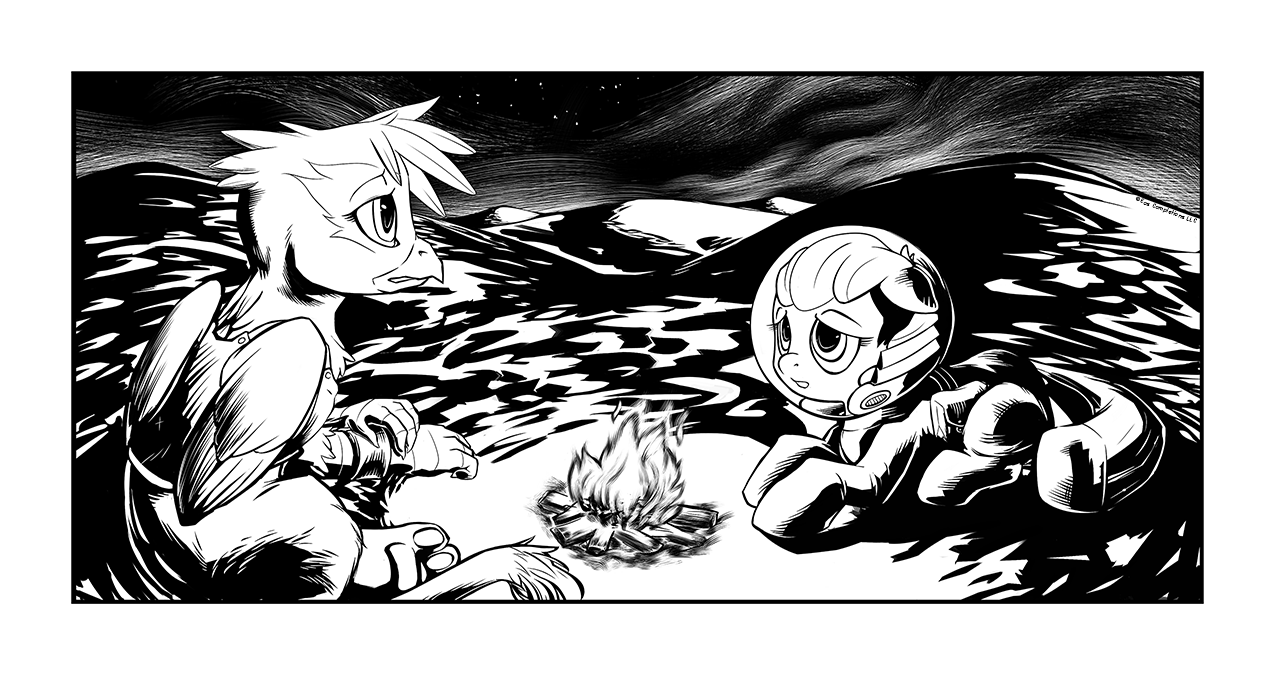
\includegraphics[width=0.9\linewidth]{image10.png}

\begin{intro}
In the desert you can remember your name, 'cause there ain't no one to give you pain.
\end{intro}


\englishdaytimeplace{9}{2:00 A.M.}{Sun City Downtown, Big 52 SC Branch}

``Fuck this headache, I can't sleep.'' Henrietta rubbed her sorry head. Puppy was a good aim, and had a fair bit of strength when it came to throwing things. Now Henri was feeling the full force of Puppy's skill. The day had been a hard one with a lot of work, dismantling the buildings in the outer belt and bringing the materials to the residential area. If she hadn't had that wound, she would have been asleep like everyone else.

``Next time I see that yellow devil, I'm going to spank her so bad that her rump could be used as a landing signal on foggy nights.'' By the way, what was she doing in Sun City? The whole place was a trap, with that hypnotic buzz that could bend your will and---

Henri's eyes widened in sudden realization as she muttered to herself, ``Wait a single eggfucking second\dots The buzz is gone. The damn buzz is gone, and I can think clearly! I've got to get out of here!'' She stood up, spreading her wings, ready to take flight, but froze in place as soon as she noticed the other griffons. There were five of them in the room. Two were the Talons that she tried to lose by diving into this fucking place, while the other three had the Talons tattoos, but wore no armor and didn't appear to be armed.

``At last, it's payback time!'' A cruel grin appeared on Henri's beak as she unsheathed her bowie knife and stepped toward the first sleeping griffon. She was one of the unarmored ones, sleeping intently because of the day's hard work. The young half-eagle moved slowly and silently, like a serpent in the grass. She approached her victim from behind, ready to grasp her beak and slit her throat. Very slowly she leaned over her victim's head and\dots noticed the eggs.

``Oh fuck no.'' The fire in Henrietta's eyes died as she looked at the two eggs that the griffon was hugging in her sleep. Rage became hesitation and her resolve shattered. Killing a mother in her sleep was beyond any hunger for revenge she had. But the other four, on the other claw\dots

The other four what? Two were just victims of the place, and one of them could have been the father of those eggs. Besides, they were totally unarmed and possibly didn't have anything against her. And the two that chased her inside Sun City were sleeping hard enough that she was going to be miles away before they realized that she was gone. What was the point in killing them like this?

``I'm not a backstabber.'' Henrietta turned on her tail and headed for the door, but stopped as she noticed a spot of pink in a corner of the room. Willy Fail, Stinky Mail, or something like that. Puppy's doll. Hell, she had almost forgotten about the doll. ``Oh fuck, Puppy!'' Stupid feather head, she had almost forgotten about Puppy!


\horizonline

\englishdaytimeplace{9}{2:30 A.M.}{Sun City Downtown, Big 52 SC Branch}

Sitting in the red shadows of the control room, Puppy was still confused. She had no idea who that mare that visited her before Mister Voice came back could be, and she wasn't sure if the newcomer was a pretty pony. Even thinking about that scary mare talking in her head was enough to send shivers down her spine. She hoped that she wasn't going to return any time soon.

Luckily enough, Puppy was now in good company again. Whatever problems the mare's voice had created were far enough away to let Puppy think about more pressing matters. First things first, she needed to find her a name, since Miss Voice was already taken.

``Ah, she's a she, so miss is okay, and she is, ah, scary? Scary Voice? Sounds wrong\dots'' Puppy frowned. This was going to be a hard nut to crack. ``Head Voice? Meh. Nightmare Voice? Too long\dots I know! Creepy Voice, because she is creepy! Yay!''

The HUD on the helmet tinged, informing Puppy that the mission ``Shaping Nightmares'' was successfully accomplished. Yes, she was good. No challenge could slow her, not even coming up with names for things. Okay, maybe something long to read could still be a mighty foe, and counting things that were more than her hooves was hard, and even opening pickle jars, that had always been an impossible feat\dots But everything else was easy, right? Go Puppy!

Now that the cheering was done, it was time to undertake part two of her master plan, finding Henri and getting out of here as quick as a pony at the Running of the Leaves. ``Okie dokie, Mister Voice, where's Henri?''

{\mt ``Henrietta Firebright set as primary target.''}

The arrow on the compass integrated in Puppy's helmet disappeared and reappeared pointing to her left, displaying a distance in meters that rapidly diminished until it reached a single digit.

``Yay! It's adventure ti---''

\emph{BLAM!}

\emph{CRASH!}

\emph{BLAM!}

One of the windows exploded, and with a flutter of wings a young griffon wielding a pair of .45 pistols blitzed inside the room through a cloud of glass and bullets. ``Hold on, Puppy, I'm here!'' She tumbled across the floor trying to identify any possible hostile target, fired twice at the lights in the ceiling, which plunged the room into darkness, and jumped behind a desk before upturning it to use as an improvised barrier, all in the space of just a few seconds.

A smile grew across Puppy's muzzle as she watched the show. Wow, this was so cool! Henri was totally the best pony! She was like that griffon in that movie, Liòn: the Professional. She stomped her hooves on the floor, cheering her friend's performance. ``Woohoo! Go Henri, you rock! Way to go!'' A couple of bullets narrowly missed Puppy's helmet before Henri recognized her friend.

``Lie flat on the floor Puppy, I'm taking care of them! Leave this little pony alone, you brain eaters!''

``Wut?'' Puppy tilted her head with a curious expression.

Noticing that nopony was firing back and that there was no movement in the room, a thought suddenly struck her. Could it be that Puppy wasn't actually in danger? Henrietta smiled in embarrassment as she stopped acting like a special forces pony and took a decent look around. Putting away her guns, she stroked back the feathers on her forehead and assumed a cool demeanor. ``Hey, Puppy, still all in one piece?''

She checked her legs and tail, then smiled and nodded to her friend. ``Yup, I forgot nothing! Is Silky Tail all right?''

``Your doll? Sure, want it back?'' Henrietta grabbed the pink plushie and waved it. Puppy shook her head.

``Nopey mopey, she is fine with you. I asked her to keep an eye on you and she warned me that you were in danger, so I came here but at the beginning you were all grumpy and scolded me then you flied away and didn't want to talk with me anymore, so I waited for the night because I had this super duper mega plan but before I had to say to the mayor that his town was ugly but then the mayor wasn't a mayor, but a stoopid voice that told me bad things, but I was smarter and he said he was sorry and now he's gone away, so I'm smarter than Blue Voice.''

Henrietta rose a claw. ``Wait wait wait! I see you moving your muzzle, but all I hear is blah blah blah. None of it makes sense and we're in a hurry. Everyone is sleeping right now, but very soon someone will wake up and realize that the buzz is gone. This place is filled with Enclave pegasi, Talon griffons, and ponies from at least two different tribes, and they are all sitting on a fortified source of pure water and fresh food.''

Puppy tilted her head in confusion. ``Uh, okie dokie?''

Henri facepalmed. ``All right, simple version. In a couple of hours Tranquility Lane will become War Zone: Sun City, and we have to get our tails out of here before that happens, capeesh?''

``War zone? Like when ponies are mean with each other?'' Puppy asked with some degree of doubt.

``Yes, exactly. Each group will want to take this place for themselves. Now, leave behind everything heavy you have in your bags because we need to get out of here, and fast.''

Puppy frowned. ``But why do they have to argue? Ponies are pretty and nice. They shouldn't be mean!'' She explained her theory about pony behavior as if it was something so simple that it was impossible for it to be some other way.

Henrietta opened her beak to reply that an entire world had turned into a wasteland as a legacy of pony kindness, but trying to explain such a concept to Puppy was harder than teaching an anvil how to swim. And even more importantly, it required time that they didn't have. ``Yeah, exactly, but we have to go away right now anyway, because you have to find your mom, right?''

Puppy nodded vigorously. ``Yush! I have to go to a peggysus fly place named Blue Idontknow, but Miss Happy told me that now it's called Something Manner. Ah, I don't remember the name very well, but there's an arrow on the compass so I can't miss it!''

Henrietta sighed. ``Let me guess, it's south.'' She pointed a direction with her claw.

Puppy stared in surprise at her friend. ``Woah, how did you know that? Are you a wizard?''

``Yeah, sure, I'm the best magician in Equestria. The Great and Powerful Henri. Now please dump everything you don't need or we won't be able to fly.'' Henri paused for a moment, noticing something new in her friend. ``Say, how long have you had a blue streak in your mane?''

A thin line of blue ran through Puppy's blonde mane, starting from her forehead just above her right eye and ending at three quarters down her neck. The line was made of a couple shades of blue, in a similar way to that mare from the Ministry of Magic, Twilight Snarkle or something like that.


\horizonline

\englishdaytimeplace{9}{3:00 A.M.}{Sun City Downtown, Big 52 SC Branch}

Puppy risked opening one eye and looked down. The world rushed away from her into the night. Large skyscrapers zipped past below her, and dark, deserted roads trailed off into the distance under her nose. Much too far under her nose to be comfortable with.

``ARE WE THERE YET?'' She grabbed Henrietta's neck tight enough to choke her.

``Ack! Loosen those hooves, pony, you're going to make both of us crash!'' At first it just seemed natural to Henri to fly away with Puppy. She was really small and, once she threw away all those useless scraps, she was lighter than a military backpack. Problems came when Puppy discovered that she hated flying. ``Just close your eyes and pretend you're having a regular piggyback ride or sing something!''

Puppy already had her eyes sealed tighter than a Stable door, but it didn't seem to help at all.  Seeing all the houses from above and seeing the roofs run and run away in a crazy stream of colors already scared her enough. This wasn't like looking down from a tower. Towers didn't go around, and they had floors! She liked floors, they were so\dots so flat, and floory! ``Please please please I will behave! Put me down pleeeease!''

``Oh c'mon, are you a scaredy pony? Have some faith in your friends!'' With a stroke of her wings, Henrietta gained a little altitude, flying between two skyscrapers and soaring past downtown, high above the residential area of Sun City. The fresh night air tasted of dust and old, but the south winds carried a new scent, the sea. ``Just relax and enjoy the trip. Sing something!''

Singing something. Yes, that always helped Puppy. She just had to sing a song and everything would be better! She cleared her throat and tried singing the first thing that came to her mind.

``
\begin{song}
	Humpty Dumpty sat on a wall
	
	Humpty dumpty had a great
\end{song}
OH PLEASEPLEASE\emph{PLEASE} PUT ME DOWN NAO!''

She was dancing the pony pokey on Henri's back, but a griffon's constitution is one of a predator, happy to fly with an adult pony struggling in her claws and still capable of gaining altitude in the meantime. ``Stop it, I'm not letting you fall! Yeow! Don't pluck me! Have you the slightest idea of how long those plumes take to grow back!?'' Sick of being pestered by the panicking pony, Henri bumped Puppysmiles off her back and caught the falling filly with her talons. ``All right, at least this way you don't risk falling! Hold on, we'll land as soon as we're out of the ruins!''

``EEEEEEP!''

``Don't wet your suit! It's a couple kilometers at most, so we gotta put some distance between us and this place before it blows up!'' She accelerated, pushing herself harder so that the trip would be as short as possible, but carrying a howling banshee in the night sky was going to wake some sleeping ponies. Henrietta could only pray to her lucky star that nopony would poke their head out a window and look for the source, or that they wouldn't care enough to bother.


\horizonline

\englishdaytimeplace{9}{3:30 A.M.}{Serpent Desert, Big 52 SC Branch}

``I wasn't scared at all, you know. I was just, ah, cautious. I mean, with all those roofs looking the same and the wind you could, ah, lose yourself, and it's much better seeing the names of the streets when you don't know where you are going.'' Now that she had all of her hooves on solid ground again, Puppy was desperately trying to regain her macho appeal, but the effort was a little wasted by Henrietta literally rolling on the road laughing.

``Priceless! You're priceless, Puppy!'' She gasped as she tried to inhale, wiped a tear from her eye, and burst into another laugh. ``How did you scream? \emph{Eeeep!} Do it again, do it again please!''

Puppy pouted, sat down and sighed. ``Hey, I wasn't the one that got lost in a city! I've seen chickens smarter than y---'' 

\emph{BLAM!}

Puppy looked down at the hole in her suit, right where her heart should be. ``Hey! There are already enough bullybots doing that!''

Henrietta got up and waved her gun in a dismissive manner. She still hadn't stopped smiling, even after she shot Puppy. ``Aw, don't complain. You got torn apart by a manticore and you're still standing! How could you get hurt by a bullet or two?'' 

\emph{BLAM!}

\emph{BLAM!}

Another couple of shots pierced Puppy, once in a leg and again in her chest. ``Stop it! This stoopid suit starts saying absurdities and mumbo-jumbos every time this happens!'' A thin thread of pink poured from the holes made by the griffon's gun.

``Okay, okay, but you stop calling me a chicken.'' Henrietta yawned and put away her pistols. ``Just for your information, normal ponies die when they are shot, even ghouls, so don't try this on other ponies, okay?''

Puppy nodded, a bit confused, then tilted her head. ``But I am a normal pony!''

``Hey, hey, I didn't say otherwise\dots Woah, are we a little upset today? Want me to sing you a lullaby?'' Henri asked with a mocking tone.

Puppy nodded vigorously. ``Sure! I lovelovelove lullabies! Can we sing \emph{Hush now quiet now}?''

Henri facepalmed. What was the point of trying to provoke this foal if she couldn't even tell when she was being mocked? ``You're a lost cause, Puppy. ''

\begin{song}
		``Hush now, quiet now, it's time to lay your sleepy head!
	
		Hush now, quiet now, it's time to go to beeed!''
\end{song}

Henri sighed and started walking south. ``Why, dad, why do I owe my life to this idiot twice?'' She smiled and turned her head toward Puppy. ``Hey, jump on your red racer, and I'll fly above you. We have a lot of ground to cover if you want to get to Rust Manor by tomorrow.''


\horizonline

\englishdaytimeplace{9}{10:30 P.M.}{Serpent Desert, Big 52 SC Branch}

A small campfire cast the shadows of Puppy and Henrietta over the sand dunes. The two travelers were sitting next to the little source of light and heat. Henri was eating something from a tin can, but from the faces she made it wasn't exactly griffon food. The clouds above the desert helped the place to maintain its temperature even during the night.

``So, Puppy, this Blue Voice told you that you're a robot?'' Henri's expression was hard to read, like she was trying to keep a poker face until she finished telling the whole story.

``Yes, and he seemed double super sure of this. I almost fell for it too, but then arrived Creepy Voice that told me that it was impossible because, ah, I didn't understand that part, but it seemed quite okay when she said it.'' Puppy nodded wisely, as if this was everything that she needed to know.

Henri shrugged. ``So, a computer tells you that you're some sort of crazy machine, but a hallucination says otherwise. I think you just got dazed by the EMP grenade because of the backlash on your suit's circuitry and you had a dream.'' Henrietta yawned before continuing. ``But I don't think you're a robot, Puppy. Robots explode when shot, and, besides, robots are intelligent.''

Puppy frowned. ``So, what do you think I am?''

Henri stretched her hind legs and took a seat on her improvised couch. ``You? You're bad news, that's all I need to know. But I like you, so you can hang with me and be cool like big sis Henri.''

Puppy trotted over to her companion and met Henrietta's gaze. Her eyes were two large glowing pink lights in the darkness of the night. ``Yes, but, I am a pony, right? I mean, it doesn't matter if I don't eat or drink or never need to potty, right? I'm a pony\dots''

\emph{She seems worried, this robot thing is actually scaring her\dots Oh, fuck, why me?} Henri was completely exhausted, and she didn't need a foal with an existential crisis at the moment. All that she wanted was to get some sleep. She patted Puppy on the helmet, yawning. ``You can be whatever you want, Puppy. You are a good pony, and good ponies are the most rare variety in Equestria nowadays. As long as you think that you should be a pony, then you'll be a pony. Now go to sleep, please.''

Puppy smiled and tried nudging Henri through her helmet. ``Thank you Henri, you are my very best chicken friend!'' Crouching next to Henri, she sighed and waited, since she wasn't sleepy at all.

\dots

\dots

``HEY! What did you mean by I'm not a robot because they are intelligent?'' Puppy poked Henri in a flank, but Henri just snickered and turned on her other side.

``Priceless.''

Puppy kept whining and poking her friend to try and make her talk, but Henri began to snore loudly, leaving a frustrated Puppy complaining in front of a dying fire.


\horizonline

\englishdaytimeplace{10}{1:00 A.M.}{Serpent Desert, Big 52 SC Branch}

It was still dark and Puppy couldn't sleep. She wasn't tired at all, but Henri didn't want to be disturbed, so Puppy did the most logical thing she could think of: sightseeing the desert by night, because wise Puppy is wise.

So far this place had deluded a lot of Puppy's expectations. After all those movies with the cowponies and the buffaloes, she was quite sure that a desert should be crowded with so many skulls, arrows, tents, and other things that you couldn't even find a place to put down your hooves. But after spending a few days in the ``real'' desert, she had the slightest suspicion that all the buffaloes must have gone away for some sort of holiday. She at least hoped to find a lizard in a place called Serpent Desert, but all she had seen so far were a couple of carts half buried in the sand, and a large parasprite with long teeth that was building something similar to a nest. When she approached it, the parasprite flew away, avoiding her.

{\mt ``Warning. Hostile detected. Analyzing: Mutated parasprite, Parador variety. Threat level: deadly.''}

``Aw, why is every pretty fluffy animal in this place so shy? I just want to make friends!'' said the two-hundred-year-old monster to the mutated, murderous offspring of Mother Nature and Father Taint.

``Hey, Puppy, it's been a while. You travel a lot, don't you?'' said a staticky voice, interrupting the little exploration of miss adventure. She smiled broadly and turned to her friend.

``Mister Questioner! Where have you been?''

``It's Watcher. I watch things, Watcher?''

Puppy nodded, still smiling. ``Okie dokie, Mister Questioner, can I watch things too?''

From the speakers of the spritebot came a soft and metallic chuckle. ``Puppy, Puppy never changes. How are you? I've heard that you had a little adventure in Tunnel Town, and now I find you south of Sun City.''

``Yush! I met a lot of nice and pretty ponies! There was this chicken called Henri, and then Asso and Sweet Flower, Happy, Jamie, and a lot of other friends!''

``Wow, you are quite lucky to have so many friends, aren't you? And say, have you been in Sun City?'' The voice was trying hard to maintain a neutral tone, but it seemed very curious.

Puppy frowned. ``Yeah, it was like a super duper box with streamers and mighty fine wrappings, but with oatmeal inside. Everypony was grumpy, they didn't want to talk with me or to play with me, and their mayor was a stoopid voice that told me bad things.''

``Bad things like what? Would you like to talk about that?'' Watcher's voice betrayed a hint of worry.

Puppy looked away. ``He told me that I wasn't a pony, but a robot, then I used that big teapot that puts robots to sleep, and I was hit too. Everypony keeps telling me that I am no robot, but why I---''

``Tut, tut, Puppy. Don't fret your little head. If there's something that I'm completely sure of, it's that you're not a robot. That voice probably read some data from a sensor scanning you, but it was a machine and couldn't see beyond your appearance. You are a pretty pony, okay? Now smile and show me that everything is all right.''

Puppy nodded and smiled a little.

``Very well. Now, zombie ponies in a nice city. Did you find anything like a buzz or a humming sound all over the place?''

``Nopey mopey, but Henri told me that the buzz was gone and that all the pretty ponies were going to wake up and start being not-so-pretty.''

``Oh, so at last the interference is gone. I can finally take a look inside the place then. Let me guess, you stopped it?''

Puppy frowned. ``No, I just went there because I was told that Henri was in danger, but she wasn't! She just acted like a stoopid chicken flying around and not paying attention to me, like every other pony in the town, so I went to this Blue Voice Mayor and we had this big argument. He wanted to be smarter than me, so I took the blue teapot and---''

``Ah, excuse me, what is this blue teapot?''

She sighed, helmethoofing. ``Why I have to explain everything to everypony? It's a teapot, round and shiny with a blue pointy head. I found it inside a rusted cart in that place in the swamp.''

``All right, so you detonated an EMP shock shell in front of a supercomputer. Yes, you stopped the interference. And what about the new look?''

Puppy tilted her head, trying to look at her mane. ``You mean the blue line? I don't know, it appeared when I woke up the other day after speaking with Cre---''

``Hey Puppy, who's there? Hold on, I'm coming!'' Henrietta's voice interrupted the little pony.

``Sorry little one, I've got to go. You can tell me this story another time!'' Without even waiting for an answer, the spritebot made a noise like static and began playing some patriotic music.

Henri quickly vaulted over the top of the dune separating her and Puppy, checking the surroundings with a gun in both her talons. As soon as she decided that there was no immediate danger, she put away the weapons and scolded Puppy. ``Bad pony! Stop playing around with the spritebots and come back to the camp!''

Puppy waved a hoof at the floating robot as if left and trotted back to her feathery friend. ``I wasn't playing, I was telling him my interesting adventures!''

``Yeah, sure. Now let's get back to sleep. Tomorrow will be a long day.'' She rubbed Puppy on the helmet and they went back to their camp.

Half an hour later, a scared parador could finally go back to building its nest in peace.


\horizonline


{\rt
Good morning fillies and gentlecolts! This is Lonesome Pony, and you're listening to Radio 52! Find a radio better than us, and I'll personally give you a treat! Who, DJ PON-3? Please, I've heard he's a she! Really! And during clear nights she transforms herself into a giant three headed diamond dog! No kidding, just go to Tenpony tower during a clear night and you'll see! ``But L.P., There hasn't been a clear night or day since the spells fell!'' Not my problem, my little ponies! You just stay tuned on Radio 52 and stop blabbering about crossdressing radio DJs!

Now, back to work. It's news time! Yesterday morning, Sun City woke up from a nineteen year long sleep. I don't have any details, but it seems that during the night somepony assaulted the central tower of the town, stopping whatever device was controlling the minds of everypony in the city! Yes my little ponies, you heard me correctly! Nopony ever came back from Sun City because the whole place was under the effect of a giant mind control device! This is crazy!

And guess what the pretty residents did the very same moment they realized that the mind control was gone? You guessed it! They started fighting each other for control of the town! If you are going to cross Serpent Desert, take a long detour, following Green Route East or take the Chasm Trail, but stay away from Sun City until things settle down! I repeat, stay away from Sun City and avoid Red Route if possible.

Now, for the ones who like a little gossip, who's responsible for the change of administration in the city? Do I really need to say the name? Yes my little ponies, our little resident hero saved you from a never ending sleep so that you could freely and willingly WASTE YOUR LIVES KILLING EACH OTHER! Don't you even feel ashamed? I\dots I don't want to talk about this. Take some music while I look for answers in an empty bottle.

What we've got here is a failure to communicate. Some ponies you just can't reach\dots
}

The voice of the DJ was replaced by music.

\begin{music}
		Look at you young colts fighting.
	
		Look at your fillies crying.
	
		Look at your young colts dying,
	
		The way they've always done before.
\end{music}

\horizonline

\englishdaytimeplace{10}{10:30 A.M.}{Rust Manor, Big 52 SC Branch}

Rust Manor seemed like exactly what it said on the tin: a large, reinforced barricade made up of huge air wagon carcasses forming a ring a hundred meters in diameter around what was originally the offspring of a bunker and an air traffic control tower. The whole structure was once coated in thick, reinforced steel plates, but now all the metal was rusted, and the large tower seemed a monument to the concept of neglect itself. Nonetheless, the little town was a lively trading post, with several caravans stationed outside of the northern gates, and half a dozen town guards scanning the surroundings from a crown of guard towers built on top of the wall.

Henrietta called after Puppy, trying to get her to stop when they were a couple of kilometers from the town, where the low hills became a flat plain peppered with craters. During the war the airfield was heavily attacked with conventional weapons, flattening every structure except the fortified control tower. The open terrain gave a sniper a long line of sight, which made it easy to take care of any possible nuisance. 

``Wait for me, red bolt!'' Henri landed in front of Puppy, making her stop and kick up a cloud of dust.

``Woah, look where you are landing! I was running there before you!''

``Yeah, sure, whatever. I need you to listen carefully, fishbowl head. I have to leave you again, but this place is safe, so you won't find troubles.''

Puppy's eyes grew large and teary while she was already starting to pout. ``But-but why? I don't want you to go away!''

``Yeah, I know. I'm cool, and without me you are quite clueless, but those guys that were after me in Sun City had a whole day behind their wings. It's possible that they're waiting for me here. I don't want you to get involved in my troubles.''

``Ah, if the bad chickens are after you we can explain to them that you are a good girl, and you will behave and say that you are sorry for whatever you did so they will let you be, can we?''

Henrietta sighed, patting Puppy on the helmet. ``The story is a little more complicated than that, involving things like me having shot a couple of theirs and them wanting my head, so\dots No, I don't think we can just say that we are sorry, especially since I'm not sorry. They killed my father.''

``Oh,'' Puppy lowered her eyes, trying hard to think of something else. ``But you can't just bully those that bully you! I mean, they're not bullybots, they're pretty kitties! You can't bully kitties!''

Henrietta snickered. ``Yeah, pretty kitties. That's why I'm not going into town. If I avoid them, there will be no need for me to kick their sorry butts, and they won't be able to bully me.'' Henri shrugged. ``And that ends the topic. Take care Puppy, I'm sure we'll meet again.'' Without even waiting for a reply, Henrietta jumped into the air, and with a couple of strokes from her wings she was already out of range of the eventual stone throw from Puppy.

Puppy galloped after her friend for a few hundred meters, calling desperately for her before stopping and sighing. ``Aw, this is not fair. She didn't even hug me goodbye!'' She raised her head to the sky, screaming, ``Silky Tail, take care of her! She's in your hooves nao!''


\horizonline

\englishdaytimeplace{10}{11:00 A.M.}{Rust Manor, Big 52 SC Branch}

The sniper had been keeping the yellow dot in her sight since she had come over the last hill, but the unicorn mare was uncertain of what she was looking at. The guard put a hoof on an interphone. ``Last Stand here, I have a contact at one, one, eight, six, south. It seems to be a pony in a yellow suit, could be that ghost from the radio, fits the description pretty well. Are ghosts welcome here?''

The speaker replied in a storm of statics and electric whistles. ``Keep an eye on the target and see what it does. Call again if you notice any hostile behavior, otherwise let it approach the gates.''

``Roger, roger.'' The mare went back to her position.

In the meantime, Puppy reached the first caravans, drawing the attention of almost every hired guard in the area outside the walls. A lot of ponies were whispering to each other, and a couple of them reached for their weapons. She didn't even notice their reactions. Her mother was somewhere inside the big town, and this was all that she needed to know. ``Hi, I'm Puppysmiles! Have you seen my mom? Mister Voice told me she is here!''

All the ponies in the area looked at her, then one of them sighed. ``Oh, it's just Lonesome's Ghost.'' The guards put away their weapons and a couple of merchants that stopped chatting at Puppy's appearance went back to their business, but nopony replied to her question.

``Uh, I guess that's a no?'' She was confused. Her status changed from center of attention to completely ignored. This couldn't be right. ``Aw, when you want something done, you have to do it yourself. Okie dokie, Mister Voice, where now?''

{\mt ``Analyzing. Loading local maps: Blue Feathers Airfield. Matching failed. Loading backup data. Finding points of interest. Points located: one---Control Tower. Control Tower set as next way point.''}

The arrow moved on the compass.

``Oh, inside the town, all right!'' Puppy trotted merrily towards the gates, but was stopped almost immediately by an old stallion wearing mercenary armor and a dusty hat. Somehow the eyes of this pony held something familiar, as if the little pony had seen them somewhere before.

\rcpr{``Hey mom, why that pony has only three legs?''}

\rcpr{``He's a war hero, Puppy, please don't bother him. He's very tired.''}

\rcpr{``Yeah, tired of giving my leg for a fucking useless war against fucking enemies I don't even care about because of a fucking goddess that puts a bunch of coal in front of a pony's life!''}

\rcpr{``Tee-hee, the pretty pony says strange words!''}

\rcpr{``No Puppy! Forget that word, it's a bad word! And you, you should be ashamed of using such a language in front of a foal!''}

\rcpr{``Fuck off, bitch.''}

\rcpr{``Let's go away, Puppy, come with me.''}

\rcpr{``But Mom, I wanted to---''}

\rcpr{``Yeah, pink rat, trot after your mom! There's nothing to see here\dots''}

Puppy blinked, lost in her memories. When she came back from her personal world, the old pony with the angry eyes was still standing there, so she stared back at him and tilted her head. ``Hi, have you seen my mom?''

The mercenary spat on the ground. ``Are you deaf or what?''

Puppy sat down, looking confusedly at her interlocutor. ``Ah, sorry I didn't hear the question. Why are you angry? Did I do something wrong?''

The pony snickered. ``I asked you if you think you're a hero or what.''

Puppy smiled, this was easy. ``Oh, I'm Space Captain Andromeda! With my space suit and my super fast ride I run all around the cosmos and meet a lot of new friends! Wanna play with me? I have a rocket too, look!'' She rose a hoof stating. ``Rocket!'' A rocket toy floated in front of her.

The old stallion raised an eyebrow. ``Are you trying to make a fool of me? Do you know who I am? You better pick your foes and lower your ears, you fucking load of shit!''

Puppy giggled. Weird words always made her giggle. ``Tee-hee, mister old pretty pony says strange words! Can I play too? I'm good at inventing words, like, ah, scootalicious! Or bananaphone!''

The small crowd of curious ponies started laughing. Puppy not only didn't seem any impressed by that old mercenary, but she was laughing at him, too. Sooner or later somepony's blood was going to stain the dirt.

Last Stand again put a hoof on the interphone from her guarding post. ``Last Stand here, there could be trouble outside of the northern gate. The yellow pony is getting into a fight with a mercenary.''

``We are sending a couple of guards. Wait for instructions and hold fire unless one of ours is attacked.''

``Roger, roger.''

In the meantime, the old pony grabbed Puppy by a leg and lifted her from the ground, looking into her eyes with a menacing face. ``So you think you can laugh at me? You think I won't touch you just because a fucking pony in a radio program talks about you? Think again!''

``Hey, lemme go! I have to find my mom! I didn't do anything to you, meanie face! Put me down!'' She was struggling, but she couldn't break free. ``If my mom was here she'd show you! Lemme go, lemme goooooo!''

Somehow the whining of Puppy killed the mood. The small crowd looked away in embarrassment, and even the old mercenary wasn't really sure of what he was supposed to do now. She wasn't some stuck up hero walking triumphantly through the city gates or some sort of knight in shining armor thinking that she had Luna knows what kind of holy mission. This was just a---``Fuck, Lonesome Pony must have gone very far with his tequila to call this critter a hero.''

In the meantime, since everything else didn't work, Puppy started crying, wailing, and whining. Even the last few ponies that had stayed, hoping to see some action, left at the sight of that murderous act against dignity.

The mercenary put her down, sighing. ``Go away, I don't pick fights with foals.'' He gave a quick spank to Puppy's behind to empathize the order, and Puppy galloped away, still crying.

Somehow, he knew that he was a bad pony, and that he should feel bad. Somewhere inside the weathered mercenary a little pony actually did feel bad, but it was just for a fraction of a second.

~\vfill

\begin{engnote}
	Level up! (9)

	New perk added: Whining Presence - You can whine your way out of almost every situation. During certain encounters you gain special dialogue options that let you avoid combat, but you'll lose reputation.
\end{engnote}



\chapter{Family Doodles}

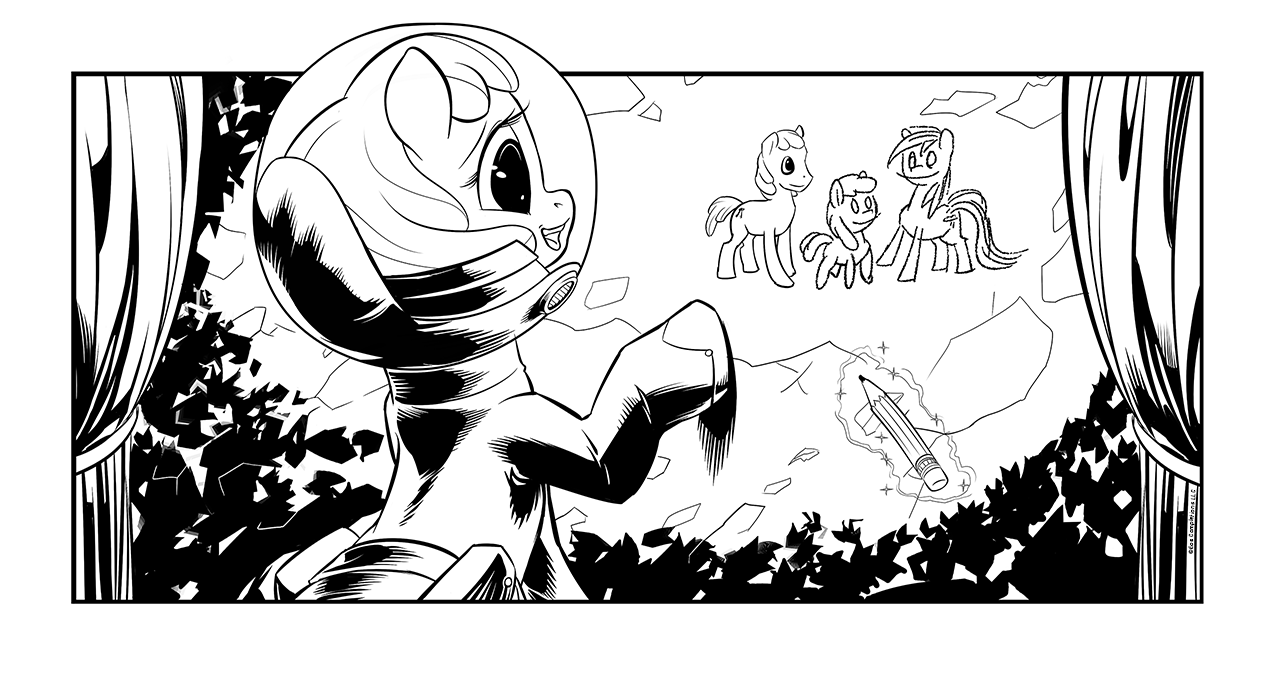
\includegraphics[width=0.9\linewidth]{image11.png}

\begin{intro}
You're not using power tools, are you?
\end{intro}


\englishdaytimeplace{10}{1:30 P.M.}{Rust Manor, Big 52 SC Branch}

\rtpr{Ahem, good afternoon everypony. I am Lonesome Pony, and this is a special edition of the news, fresh from Dust Manor.}

For a moment, the feminine voice of the afternoon DJ could be clearly heard in the background yelling ``Gimme back my seat you hog!'' followed by a metallic sound.

\rtpr{DJ Good Stuff will be back immediately after the news. I mean, what kind of a name is Good Stuff anyway? What are you, a Mintals table- ow ow OW, stop that! All right, I was kind and sweet, but now you asked for it! Here comes love and tolerance, Minty!}

A muffled sound that resembled a brawl interrupted the program. After about a minute, Lonesome Pony began to talk into the microphone again, trying to hide his panting.

\rtpr{Good Stuff wishes you well and will be back in a minute, but at the moment she has her hooves tied\dots with a power cord. So, where were we? Oh right, the special news! This is fresh from not even an hour ago, from my radio friends in Rust Manor! Thank you Easy Filly Butterfly 23!}

Lonesome Pony cleared his voice and started talking.

\rtpr{Some heroes fall, some heroes get killed, and some heroes disappear into a Stable and never come back. Well, our hero gets spanked. Yeah, you heard me. Late this morning the Ghost was sighted outside Rust Manor heading for the town, and when she tried to approach a group of caravans, a guard scolded her and spanked her in front of everypony. Now, are you fucking idiots or what? From the little we know, this pony destroyed a fortified barn outside Redtrotter's territory, and ran inside a heavily guarded tunnel, frying the robot guards inside. Yes, I got some more info about Tunnel Town. The local guard chief Trigger Happy was present, and she says that the foal destroyed six sentinels using only a stone as a weapon, and you pick a fight with this foal? What was that, were you tired of living? Anyhow, it seems that the guard won the fight, if you can call that a fight. Little Miss Yellow tried a friendly approach, got a spank in response, and ran away crying.}

There was a sigh followed by a long pause.

\rtpr{Yeah, this is what I call gratitude\dots L.P. closing. Have some decent music while Good Stuff unties herself. I've got to fly if I want to live. Stay classy, Big 52.}

Music filled the silence.

\begin{music}
		Saw you stretched out in room Ten O Nine
	
		With a smile on your face and a tear right in your eye.
	
		Couldn't see to get a line on you,
	
		My sweet, honey love.
\end{music}

Puppy hid behind an abandoned cart, still crying. What did she do this time? She tried really hard to behave and be a good pony, but everything she did seemed to backfire on her. From taking a simple peek into a tunnel, to battling crazed partying robots, to roofs falling on her head---she was a magnet for bad luck. Why did Mom have to keep moving? Why wouldn't she wait for her? She felt empty and tired.

\begin{music}
		Zebra jewelry jangling down the street,
	
		Make you shut your eyes at every filly that you meet.
	
		Couldn't seem to get a high on you,
	
		My sweet, honey love.
\end{music}

But Puppy couldn't simply stop searching and sit down. Even if ponies were unkind and the road seemed endless, her mom was somewhere just over the next hill, or maybe the hill beyond that one. One hill after another, it was only a matter of time.

\begin{music}
		May Celestia shine a light on you,
	
		Make every song your favorite tune.
	
		May Celestia shine a light on you,
	
		warm like the evening Sun
\end{music}

Puppy got up. Moping behind a cart wasn't going to find Mom. She was a filly on a mission, so everything else didn't matter. Go Puppy!



\horizonline

\englishdaytimeplace{10}{1:45 P.M.}{Rust Manor, Big 52 SC Branch}

The two stallions guarding the gates exchanged a rapid glance, seemingly uncertain about whom should deal with the approaching foal. Finally, the older one addressed her. ``Sorry kiddo, if you want to get inside you have to pay. Two-hundred caps and leave all your weapons here.''

Puppy frowned. Two-hundred was a super duper big number. She was quite good at counting up to four, and with some help (and time) even ten, but two-hundred? What was a hundred anyway? ``Ah, I'm just looking for my mom, Puppy please?''

``Show me the bottle caps and we have a deal, filly.'' The guard yawned, trying to maintain his neutral tone, but he was concerned about what would happen if she didn't have the cash and still insisted on going inside. Maybe it would be a good idea to call the chief\dots

``Pouch!'' A large bag floated in front of Puppysmiles, and she handed it to the guard. ``Ah, can you help me counting these ones? Are there enough shiny caps?''

The stallion nodded and emptied the bag on a table. It was two-thirds full of caps and a third in bits from the old age, and some of them were golden. ``All right, this is more than enough.'' The pony blinked at the other guard, who cocked his head and looked back at him with a snort of disapproval. ``C'mon, she's just a foal, you can't be serious!''

The first guard sighed and counted out exactly two-hundred caps, putting the rest back in the bag and giving them back to Puppy, who smiled and put away her possessions.

``Thank you super much, mister pretty guard ponies!''

Inside the walls, Rust Manor was cramped and crowded. The air wagons used to build the walls doubled as houses and stores, leaving little space to move around the large fortification in the middle of the town. Now that Puppy had taken a better look at the whole place, it seemed like a village of tiny creatures built all around the trunk of a dead tree, only the tree was a hundred meters tall. She trotted around, peeking inside the shops and trying to find a door to get inside the fortified tower. The arrow was pointing exactly in the middle of that big thing, so it was obvious that she needed to get inside somehow.

There were a lot of ponies. Some of the locals looked at Puppy with interest or curiosity, but they were mostly minding their business, tagging her as an innocuous oddity, especially after her ``duel'' with the mercenary that morning. Puppy didn't care at all. At last, she had found a place full of pretty ponies that behaved like real ponies, and she knew that where there were big ponies working, there must be---``Yush! Ponies playing!''

A trio of foals, a filly and two colts, were running around, laughing and yelling at each other. They were having so much fun! But Puppy had to go and find her mom. But if she went away and the pretty ponies went away, she couldn't play, and she wanted to play so much! But Mom\dots Maybe only a minute, just to make friends and ask if they had seen her mom? Yes, right! She wasn't going to play---ah, talk, not play, talk---with the pretty ponies because she wanted to have fun, it was because they could know where Mom was! Ah, clever Puppy, she could even outsmart herself.

``Hi, I'm Puppysmiles! Have you seen my mom?''

The trio of foals stopped running and yelling, turning toward the newcomer as if they were all one single pony. The filly was a gray unicorn with a pink mane, while the two colts were a unicorn with a palette very similar to the filly's and an earth pony with a brown mane and a green coat. They stared for a long moment at Puppy, both in amazement and concern. Then the filly asked, ``Where did you get that super creepy space suit?''

Puppy frowned. ``It's not creepy, it's Space Captain Andromeda's Space Suit!'' At this point Puppy made a theatrical pause to raise the tension, and added, ``It's cool!''

The unicorn colt nodded. ``Yeah, I have an Andromeda comic. She's a girl, but she's super cool all the same because she has a laser gun and fights zebra aliens.''

The other two foals nodded when the expert gave his approval, and the unicorn filly smiled in a friendly manner. ``I'm Big Deal,'' pointing a hoof at herself, then, waving her hoof at the other unicorn, she continued, ''he's my twin brother Ricochet, and he's Painkiller.''

``And I'm Puppysmiles! I come from Canterlot and I'm looking for my mom. What were you doing? Playing? Can I join?'' Great, now that she asked what she had to ask twice, she could take a pause, right?

Ricochet tilted his head. ``Your mom? What's her name?''

``She's called Rainy Days and she's the coolest pony ever! She can cook muffins and cupcakes and chocolate pudding and apple pie, but she makes me always eat alfalfa. She went away some days ago for work, and then our house in Canterlot collapsed, and I'm looking for her because Mister Voice knows where she is, so it's better than waiting for her inside a collapsed house, I think.''

The three little ponies nodded, as if Puppy's speech made sense. ``Yeah, last time I broke a bottle Mom was really mad. I don't want to know how mad your mum will be when she finds out you broke the whole house.''

Puppy frowned. ``It's not my fault! I went to sleep and when I woke up the house was gone!''

``Tell that to your mom---I tried to say that a band of slavers broke the bottle but she \emph{knew}! Moms have some sort of super sense that tells them who did what,'' added Painkiller, muttering the last words as if it was better not to divulge too much of such secrets.

``I didn't break my home! Cross on my heart!'' Puppy insisted on defending her position, mostly because it was the only defense she had. Nopony was around when the house collapsed, and she was \emph{almost} sure that it wasn't her fault.

``You better have not,'' cut short Big Deal, ``but I don't know any Rainy Days living in Rust Manor. We were playing cowponies and zebras, want to join? You can be the alien.''

Painkiller protested. ``I don't want to be the zebra anymore! Why can't you two be zebras for once?''

Ricochet tapped his sister's horn with a hoof. ``Because zebras don't have horns, duh!''

Puppy intervened in the discussion. ``Once I was told that zebras can grow wings with some sort of weird device, but they're bat wings. Besides, I want to be Space Captain Andromeda.''

``But you don't have Andromeda's gun. You could be Maripony, the second mare on the moon!'' said Ricochet. His sister interrupted him.

``Maripony had never been on the moon for real! A pony can't get there!''

``Yes she did!''

``No she didn't!''

``Yes she did!''

``No she didn't!''

The twins stood in front of each other, muzzle against muzzle, arguing about a two centuries old moon landing. Painkiller approached Puppy, sighing. ``They'll go on like this until dinner. So, ah, you've got a cool suit. Does it have a compass and healing spells?''

Puppy watched the brother and sister show for a moment, then moved her attention to the earth pony. He was a little older than her, and he already had a cutie mark of a syringe. ``Are you, ah, going to make injections to me?''

The colt stared, a bit confused at Puppy before realizing that she was talking about his cutie mark. ``What? Oh, this! Don't worry, dad doesn't let me touch his stuff. So, uh, you're quite cool, for a filly\dots''

Compliments always worked on Puppy's ego. She sported a broad smile, instantly growing ten centimeters taller. ``Well yes, I'm cool, I know. Yeah, this space suit has everything! A compass, a lot of dots here and there, and some writings, see?'' She poked at the helmet, trying to show the colt all the stuff she said. ``And look at this! Ah-hem. Rock!'' \emph{The Rock Of Destiny} floated in front of Puppy.

``Woah, how do you do that without unicorn magic?''

She shrugged. ``I don't know, the suit does all this cool stuff for me. It's magic, I'm not going to explain that.''

He tapped his chin, thinking. ``Too bad you don't have Andromeda's laser gun, but I have an old toy gun I never used because it's so heavy that I can't hold it in my teeth. Maybe with that levitation thing it could fit with your costume.''

Puppy's eyes grew as large as soup bowls. ``Really?''

``Yeah, maybe if you have something to barter with, we could make a deal. I don't want it anyway. It seems girly and does nothing.''



\horizonline

\englishdaytimeplace{10}{3:00 P.M.}{Rust Manor, Big 52 SC Branch}

While Painkiller looked at the pile of 42 muffin boxes, not believing his luck, Puppy tried to point at something with her brand new laser gun. It was a pistol with a futuristic look, an antenna on the muzzle, and some metallic rings here and there. The grip had no trigger, and the whole object was silvery gray with red plastic inserts.

``It's heavy,'' she complained, trying to hold it with a hoof to no avail.

``Hey, no refunds!'' He was dropping one box of muffins after another from his grasp. ``Why can't I hold all these muffins?''

In the meantime, Puppy aimed at the sky, sitting on her rump and using both hooves to hold the weapon. She said just one word. ``Bang!''

{\mt ``New equipment detected: Sol. Inc. Prototype 152, Codename Sentenza. Synchronizing. Opening communication bridge with Comm Station n° 2. Checking status. Ponymedes net online and operative at 12\%. Relaying coordinates.''}

``Aw, this stoopid suit is talking nonsense again!''

From the curtain of clouds appeared a thin red line of light, then a second and a third. They were faint laser beams, piercing the leaden skies and illuminating with tiny and seemingly innocuous red dots a roof here and a cart there. A dog that was napping under a bench chased one of the dots across the street before banging his muzzle on a door.

{\mt ``Warning. Ponymedes 4, 6 and 7 are not responding. Ponymedes 8 to 12 cannot lock on target. Warning. Power up sequence delayed by---Impossible to deliver an estimate.''}

Painkiller didn't pay attention to Puppy, already trotting away and leaving a sweet trail of muffins behind him. ``Yeah, whatever, it's been a pleasure bartering with you.'' 

Sometimes the combined effort of a community can save a town, some other times a hero has to show up and fight their battle, and there are even times when it's just a matter of blind luck.

{\mt ``Warning. Losing signal. Abort command. Repeat: abort command. Closing communication bridge. Ponymedes offline due to recalibration, orbital relocation, and maintenance. Estimated downtime: 24 hours.''}

Finally, the suit stopped talking. Puppy snorted. ``Hey, have you finished with all this blah blah Idontcare? We have to find Mom!''



\horizonline

\englishdaytimeplace{10}{3:30 P.M.}{Rust Manor, Big 52 SC Branch}

``Oh yeah? And you're a stinky fish!''

``Oh yeah? And you are so uncool that even your cooties flee from you!''

Big Deal and Ricochet were still standing muzzle against muzzle, arguing about something they probably didn't even remember.

``Oh, that should explain why you have so many cooties! You're like a walking flea circus! Hi Puppy.''

``And you are all girly and smoochy and all you do is girly and all your toys are girly and---hi Puppy---and you are a\dots a\dots a \emph{girl}!''

``Hi Rico, hi Big D.'' Puppy waved a hoof, trotting past the twins, at last finding an entrance to the tower. The sign on top of the building let everypony know that it was a really classy brothel. As if Puppy cared.

The place was filled with red drapes, and was scarcely illuminated in an effort to hide the worn furniture. In front of the entrance a mare was sitting behind a counter. She usually greeted the customers, but now she was staring surprised at the little pony in front of her. From Puppy's point of view this was a nice place, with a lot of fancy things like posters and marble statues of ponies.

``Ah, hi there. I don't think this place is good for you.''

Puppy smiled and waved a hoof. ``Hi, I'm Puppysmiles! Mister Voice says that my mom is in this place!''

The mare looked slightly concerned. ``I\dots can't say that's impossible, actually. I have a couple of new girls working here. Do you know your mother's name? No little one, don't touch the statue, it's fragile! Ah, don't look at it, either!''

Puppy was already exploring, having found an interesting statue of a stallion in a very, ah, manly pose. She frowned. ``I think this pony has too many legs. Ah, she's called Rainy Days! And she is---'' 

``I'm sorry little one, there are no Rainy Days working here, but if you want to be sure---don't touch it!---I can call the new earth pony working here, just in case. HEY HOLLY, COME DOWN!'' Very classy brothel indeed.

Puppy wasn't listening to the mare anymore, her eyes now staring at some faded crayon lines on the wall, half hidden behind the statue.

And now she was staring at the same wall, only two centuries earlier.

\rcpr{``Wait here, Puppy, Mom will be back very soon. This will take just a few minutes!''}

\rcpr{``Okay Mom, I love you, bye bye!'' Mom nuzzled Puppy behind the ear, making her giggle before trotting away.}

\rcpr{The big room was so gray and sad, with just a couple of seats and a low table filled with ultra boring magazines showing weapons and stoopid soldiers on them. Puppy sat in front of the wall, looking at the gloomy empty space in front of her. This needed changes. This needed crayons!}

\rcpr{It took a lifetime, at least ten minutes, but now Puppy's masterpiece was almost finished. There were the two prettiest ponies she was ever able to create. One was little and pink, with a bright yellow mane. Puppy was particularly proud of how she captured her own pinkness. The second pony was bigger, with a purple coat and an orange mane. Mom\dots She was beautiful. If only Puppy could draw how beautiful she was. Oh well, the drawing was already doing a great job anyway. She had added some trees to the scene, both green and yellow, and one was pink with a yellow trunk, because she always thought that pink would be the best color for a tree. She looked over her work to see if something was missing: sun, check\dots butterflies, check\dots muffins, check\dots}

\rcpr{Now the picture needed only one last thing. ``And when we are done we will go to Dad's place and he'll be back, so we will be happy forever!'' She knew what was missing, but she was still unable to finish the picture. ``What are Dad's colors?''}

\rcpr{``Puppy, what the hay are you doing? You can't draw on walls! What did I tell you a---''}

\rcpr{``Mom, I can't remember Dad's colors.''}

\rcpr{Mom fell silent immediately. Puppy was still looking at the drawing, trying not to lose the inspiration, but how could she draw a pony if she didn't know what colors to use? Suddenly, Mom hugged her so tightly that she gasped. ``Don't worry Puppy, I swear that this will end one day, and we, we will be happy together, as we were before this war. I\dots I\dots''}

``Hey, little one, wake up, pay attention! Is this your mother?''

Puppy turned her head toward the proprietor of the brothel, now accompanied by a young mare that she didn't know. The young prostitute looked at Puppy in confusion and cocked her head. ``No, she's not mine, I would remember having a foal. Besides, I never had any pink in my family.''

``I-I've been here, it was\dots'' Puppy tried to remember, but it wasn't easy. It was as if the memories she wanted to reach were much farther away than she thought. ``A month ago, I think, but it was different.''

The matron snickered, patting Puppy on the back. ``I don't think so, little one. I've been the proprietor of the Velvet Pearl for fifteen years, and I've never changed so much as a single doorknob.''

She went back to looking at the little drawing again and finally noticing something different, something new. A broad smile appeared on her face. ``I\dots I remember him! He was white and yellow! Dad was white and yellow!'' Puppy pointed a hoof at the picture, turning toward the two mares. ``That's my dad, see? He's my dad. I didn't remember his color, but now he is there with me and Mom! There is something written here, please read it please, please, please!''

The old mare lowered her head, looking at that drawing for the first time in her life. It wasn't as if she had never seen it, she just couldn't give a buck about a stain on the wall, choosing to cover the mess instead of painting over it. The drawing was of three ponies. Two were clearly the work of a foal, just some colored lines on a wall, with some trees and a green line to represent the ground, but the third one seemed like the work of somepony good at drawing. It showed a young white stallion with a golden mane, very similar to the mane of the filly who stood looking at the wall.

Under the drawing somepony had written a few words that the old mare read in a low voice, almost whispering. ``Together again, here and forever. Love, Mom.''

Puppy put a hoof on the painting. ``Mom was here, and now we are all here! This is me, and this is Mom and this is Dad! Wait, I know!'' She reached for a pencil and added one last detail to the work: three smiles on the pony's faces. ``Now we are all happy! Yay! We can have a picnic and chase butterflies and wait for the fireflies and Mom and Dad will kiss me goodnight. It's all right again!'' Puppy paused, staring at the image as if she was living through the story she told.

The younger mare stared at the scene in silence, her face betraying a growing angst. That, that foal, how could she endure all this? That childish drawing on the wall was all that was left of her family, yet she was still smiling as if it was real. She was \emph{smiling!} But, but they were dead. She had already lost everything. She was alone! A little ghost drifting forever from place to place, asking for something she could never have back, all without rest or hope, a hole filled with faint memories, forever. The prostitute was overwhelmed by that sense of despair and eternal nothingness. She needed fresh air, to be out of that place, away from that haunting vision! She broke into a gallop, leaving the brothel behind as tears rolled down her cheeks.

The older mare was made of sterner stuff. She had already seen much of what the Wasteland could throw at her, and endured loss many times in her life. ``Yes, little ghost, you are all together.'' This was unfair. A lost foal finding a spot of happiness behind the statue of an aroused stallion was a cruel way for the Wasteland to serve you some relief. Nonetheless, there were moments like these that healed wounds, and gave you the will to go on. Letting them slip away was worse than denying yourself.

``You can sit here and watch the painting as long as you want, but I don't think that your mom is here. She must have, ah, moved away a long time ago. I'm sorry, kid.'' The mare raised her voice. ``And somepony come down here and move that statue, there are foals here! We are not perverts!'' The sensation was weird, but refreshing. That little foal, that clueless lonely soul, made her wish to be a better pony somehow. A bittersweet smile appeared on the mare's wizened muzzle.



\horizonline

\englishdaytimeplace{10}{4:45 P.M.}{Rust Manor, Big 52 SC Branch}

``Prepare your muzzle! I'm giving you a black eye!''

``Oh yeah? You and what army?''

``I don't need an army, I already have a dumb brother! Hi Puppy.''

``I'm not dumb! Hi Puppy. You're dumb! Dumber than your rump!''

``Hi Rico, hi Big D.'' Puppy trotted past the twins, who were still standing muzzle to muzzle. She had no time to assist the fight. She was looking for the place the arrow was pointing at. ``Ah, Mister Voice, what do we need to do now?''

{\mt ``Actual priority is to investigate Rust Manor. A set of public places have been selected in order to ask as many ponies as possible for information. The first location in the list is Red Water Saloon.''}

Puppy trotted inside the saloon. It consisted of a large hall with a loft at the bottom, noisy and full of hardened ponies that swore and drank hard stuff like Wild Pegasus and Coyote Tequila, sometimes mixed together and reinforced with special ingredients. To Puppy, this place was simply another room full of pretty ponies that could know where her mom was, so she went for her usual routine.

``Hi, I'm Puppysmiles! Have you seen my mom?''

For a single moment all the eyes inside the place turned on the entrance. The barpony crouched behind the counter and the pianist stopped playing, the only sound in the whole place was that of the swinging doors creaking behind Puppy.

One of the really tough ponies that was sitting at one of the tables next to the entrance tipped his hat and muttered in a voice that in the still silence was perfectly audible to everypony. ``This ain't a place for ya, little pony. Now go play with the foals before you get spanked\dots again.''

All the saloon exploded into laughter, every single pony, and since everypony was laughing Puppy laughed too. ``Tee-hee, very funny. Ah, I don't get it, but it's funny, so, have you seen my mom?''

Most of the ponies didn't hear Puppy, but two of them did. A ghoul that was standing next to the door, and the pony that had spoken to her. The former simply got out of the place, while the latter sighed and facehoofed. ``No, no I don't know where your mom is, now please go away!''

Trotting outside the saloon, Puppy smiled. Okay, her mommy wasn't there, but all the ponies in that place seemed crazy, so it was a good thing that she wasn't there! ``Okie dokie Mister Voice, what's next?''

``Hey, you there with the yellow suit, wait a moment!'' A voice from the other side of the street made Puppy stop and turn on her tail. There was a ghoul pony wearing a leather hat and a long black trench coat looking at her. ``Yes you, I have to speak with you!''

Puppy sat down in the middle of the street, tilting her head. ``Uh, okie dokie?''

After crossing the street, the ghoul patted her on the helmet. Now that he was near enough, Puppy noticed that he seemed like some sort of mummy, devoured by the sand and dried out like a big leather pelt wrapped around a carcass. Saying that he was ugly would be an understatement, but Puppy had already dealt with ghouls, and she knew that they could be nice ponies. Maybe not pretty, but nice. For a moment she wondered if Soft Air and the others had already found a new home. Maybe they'll write her a letter or, even better, send her a postcard with some super cool photo. Puppy loved photos.

The mummified ghoul cleared his voice before talking. As with every other ghoul she had met, he seemed to speak through a throat filled with jelly. ``Good girl. You are the foal Lonesome is making a big fuss about, aren't you?''

``Wut?'' Puppy giggled. ``Tee-hee, ugly pony says fancy words!''

The ghoul rose a decomposed, perplexed half-eyebrow. ``Ah, you can call me Molten Gold. I'm an adventurer and a treasure hunter.''

She smiled back. ``Hi, I'm Puppysmiles! Have you seen my mom?''

A faint smile appeared on the ghoul's muzzle. ``Mmmmmmaybe. What would you do for me if I had?''

Puppy jumped on all her hooves, ``Anything! Please please please where is she?''

The smile on Gold's face broadened. ``Good filly. I think we can make a deal, here.''



\horizonline

\englishdaytimeplace{10}{11:00 P.M.}{Solaris Stable, Big 52 SC Branch}

The cave was dark and filled with the bones of a number of different animals, but mostly just pony bones. It seemed like a macabre carpet laid on the floor of hell's atrium. Puppysmiles stepped into the shadow, followed by Molten Gold. ``I don't like this place. It's dark and full of hurt ponies, why do I have to go there?''

He sighed. The walk with her from Rust Manor to the Solaris Stable had been a torture. This foal just couldn't shut up for a single moment, but what if what Lonesome Pony said was real? Then she was also some sort of unstoppable raiding machine, able to deal with heavy defenses with little effort. ``Because I'm a treasure hunter, and we are going on a treasure hunt. You said that you like to treasure hunt, didn't you?''

Puppy frowned. ``Ah, yes I like playing treasure hunt, but usually Mom hides the cookies inside the jar, on the table. Where is the kitchen in this scary cave?''

``This time we're not after cookies, Puppy. Inside this place there is a thing I need, and if you find it I'll tell you about your mom, so listen carefully.''

Puppy sat down, trying to take a martial pose. ``Yush! Space Pony Puppysmiles ready for the mission!''

He snickered. ``That's the spirit, filly! This is a secret base built by those good for nothings from Solaris Inc. It was meant to work more or less like a Stable, but buck me if they ever made something that worked as intended. Anyhow, that is not our problem. Our problem is the fact that it's more defended than a ranger's base, but from what I heard this could be a piece of cake for a badass like you.''

Puppy mumbled, trying to find a sense in his words. ``Ah, I like pie?''

Molten laughed. ``You remind me of a very young Soarin. Anyhow, I'm not sure how big this place is, but there must be a place named `research area', okay? You have to reach that place.''

``Okie dokie! Re-search area, got it! Search it twice!'' Puppy nodded enthusiastically.

``Exactly, and when you---no no no NO! Not, search twice! Research, as in science! Now, you just have to ask your suit. It's really easy! Now repeat with me: Research area.''

``Ree-search area?'' she tried, sounding a little dubious.

``Good girl. Now, when you get there, you have to find a box filled with these.'' Molten took a round object from his bag and showed it to Puppy. ``It's called a memory orb, okay? Repeat with me: memory orb.''

``Murmuring orb.''

Molten's face deflated. ``How in Equestria have you survived this far? Memory, like remember things!''

``I know what memory is! But that's a glass ball, it can't remember things, \emph{duh}!''

He rose a hoof while his eye started going twitchy twitch. ``Wait, wait a second here please. I'll be back in a moment.''

Molten Gold headed outside, and even from where Puppy was sitting she could clearly hear him screaming, ``Why is it a fucking retarded foal, why? FUUUUUCK!''

Since the screaming seemed to go on for a while, Puppy decided to take a look around by herself, just to get acquainted with the place. The cave was large enough for a cart to pass through, but the entrance was half collapsed, so that only slim ponies could actually squeeze in. It had been easy for Puppy and Molten Gold, but if an average stallion would have tried to get inside, he was going to get stuck in the middle of a bunch of half collapsed and unstable rocks at the bottom of a narrow canyon exactly in the middle of nowhere.

The bones that littered the ground were old, white, and bleached by time and the dry climate. Some of them still sported a piece of clothing, like laboratory coats and some bits of scorched armored saddles. Rummaging through the piles of bones, Puppy found a cool pair of glasses and some shiny bits. Lucky Puppy! There were even some weapons, but she already had her super cool space pistol and didn't need some noisy and ugly toys like those. Instead she took the blue plastic card from the neck of a skeleton. Blue wasn't her favorite color, but it had that cool image with the white alicorn stallion, and she liked cool things.

When Molten Gold came back, he seemed a lot happier. ``All right, I'm done, where were we?''

``Ah, the glass balls?'' tried Puppy uncertainly.

``Yes, right, the mem---glass balls. Those.'' Molten smiled and focused on what she was holding in her hoof. ``Say, where did you find a security pass?'' His eye once again started to dance the pony pokey. ``No no no, don't tell me, I don't want to know. So, let's see if you understood. First you have to go to the\dots''

``Ree-search area.''

``Yes, and you have to look for the\dots''

``Glass balls.''

``Perfect. Now go and don't come back until you have those damn orbs,'' he said, sighing with relief.

``Okay. I like you, Mister Ugly Gold! When I find Mom, I'll tell you that you were nice with me!'' She trotted away, heading for the bunker's entrance.

``It's Molten, not Ugly\dots Aw, who cares. Just do this job so I can forget this story forever.''



\horizonline

\englishdaytimeplace{10}{11:45 P.M.}{Solaris Stable, Big 52 SC Branch}

The entrance of the bunker was a gigantic, circular door two meters thick and six meters wide, with the usual symbol of the company in the middle of it on both sides. Even here there were skeletons on the ground, littering both the floor of the cave and the entrance hall of the Stable. The hall was illuminated by flashing red and blue lights from four lamps on the ceiling, a clear sign of danger.

``Uh, pretty lights!'' Puppy jumped over the reinforced door and trotted around the hall for a moment. There were skeletons even here, on the inside, as well as destroyed sentinels. The whole place was peppered with bullet holes.

Other guns, other ragged dresses, bones, boo-ring. ``Say, Mister Voice, where is that ree-search place? Are we there yet?''

{\mt ``Negative. Current location: Solaris Stable Entrance Hall. Downloading local maps. Warning. All blueprints for Solaris Stable are protected. No maps available. Direct navigation is required. Auto-mapping function activated.''}

``Ah, this means you have no idea where we are going?''

{\mt ``Affirmative. Current location is partially unknown. Impossible to set navigation points to the objective. Please proceed with caution.''}

Puppy's eyes widened in surprise and glee. ``There's something you don't know! YAY! Who's the smart pony now, who? Ah? Ah? Who is? Not you, Mister Voice! Bleh!''

{\mt ``Warning. This program is not designed to feel bad. Any form of teasing will be reported to the Legal Department as infringement of the license agreement per section 2, article 9, comma 12.''}

Puppy frowned. ``Hey, stop using smart words I don't know! I'm not stoopid! I'm a smart, pretty pony, and when I get big I will be as intelligent as Pinkie Pie! Now let's find this place. Since \emph{you} don't know where it is, \emph{I} will have to do all the work as usual.''

From the main hall there was only one passage that led into the underground complex. Maybe this whole ``find the glass balls'' thing wasn't as hard as it seemed. After all, the place was still illuminated with the flashing blue and red lights, so it wasn't very scary. The walls were painted in a light shade of blue with a gray line, and the floor had sweet white and black tiles, so Puppy started playing with them, jumping only on the white ones and avoiding the black tiles because they were super scary bottomless pits. Hey, it was fun! ``Yay, I'm Daring Do! Look at me! Now I'll---''

``STOP RIGHT THERE, CRIMINAL SCUM!''

Puppy sighed. She never lifted her eyes from the floor. It was too good to last, she had to know that. ``Please, Puppy please! Do not start being bullybots! I don't have time for this! I have to find the balls and then find Mom!'' She tried her best pretty face, looking at the sentry bot with the two most sorrowful eyes she could give.

``SURRENDER NOW AND BE ANNIHILATED!''

The twin miniguns on the sentry pointed at Puppy, then suddenly the visor of the robot turned from red to blue and its voice changed. ``You again? What are \emph{you} doing here?''

Puppy was already asking for \emph{The Rock Of Destiny}, but at that turn of events she tilted her head, a bit uncertain. ``Mister Blue? Is that you?''

\clearpage

~\vfill

\begin{engnote}
		Level up! (10)
	
		New perk added: Finesse - No puppy, not there, please! +5\% critical chance
\end{engnote}



\chapter{Darkness}

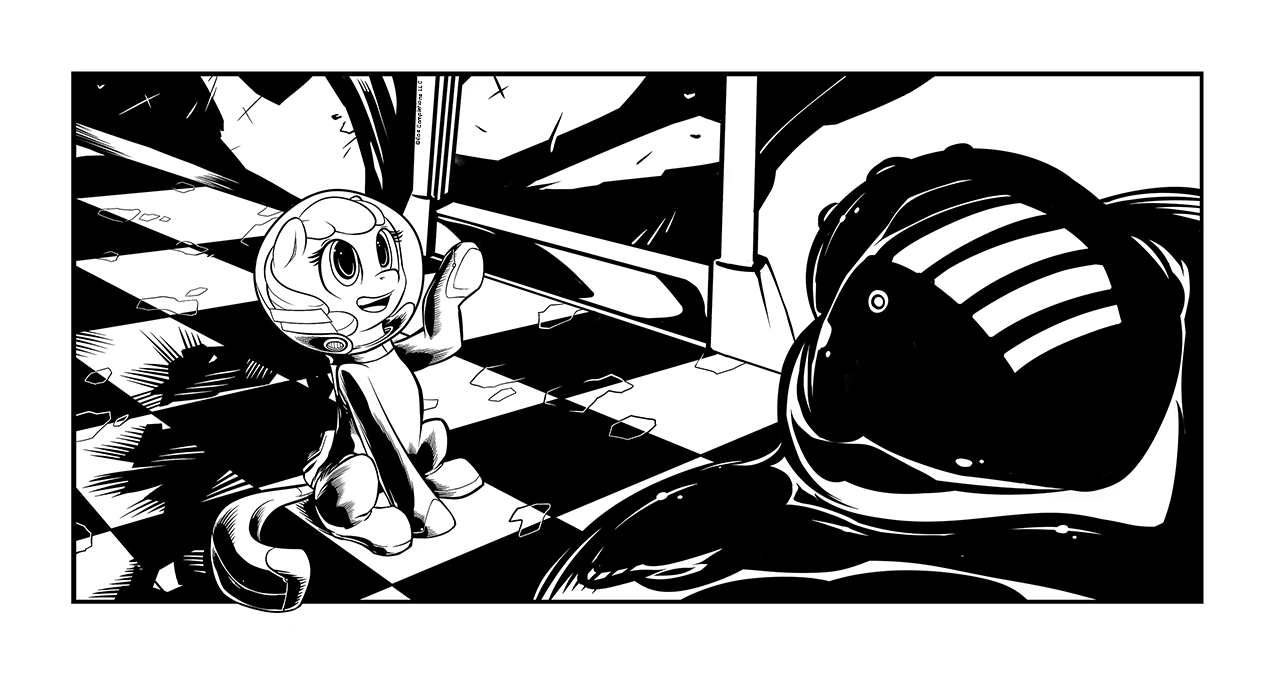
\includegraphics[width=\linewidth]{image12.png}

\begin{intro}
    When I'm walking a dark road I am a mare who walks alone.
\end{intro}

\englishdaytimeplace{11}{00:15 A.M.}{Solaris Stable, Big 52 SC Branch}

``Get out of my Stable, NOW!'' SolOS' voice thundered through the corridors of the underground complex like a wave crashing on the shore; the order came from every speaker and every operative sentry patrolling the abandoned halls.

Puppy sat down on a floor tile, making sure that it was a white one; you know, since the black ones were still bottomless pits; you couldn't let adults get in the way of playtime all the time. ``Why?''

``Because you have already caused enough trouble, you malfunctioning little drone!''

Puppy frowned. ``I am not a throne! Don't try sitting on me, stoopid Voice!''

``Drone means robot! You don't even have a decent integrated dictionary! Your uselessness makes my sub-routines reboot!''

Now, that was too much; Puppy stood up and looked at the sentinel in front of her with a really, really angry stare, but the best she could manage had the same effect as putting a military helmet on the head of a plushie\dots scarier? No, cuter. ``Hey I am no robot! Miss Creepy Voice told me, and Mister Questioner and Henri, so it's one against\dots ah\dots'' Numbers, why everything was always heading to numbers? ``Against a lot of us!''

``Many wrong results put together don't become true out of sheer magic, Device 018. Even now every sensor analysis gives the same results as before. You are a suit filled with the remains of a corpse, mostly broken bones, and a large amount of a gelatinous substance. There are no scientific studies confirming the existence of the fabled marshmallow ponies, ergo you are a crazed machine filled with goo and bones.''

Puppy raised a hoof, pointing it at the sentry. ``Stop being smart, Blue! Or else I'll have to show you again who's the gee- jeen- ah\dots super duper egghead here!''

``I don't think there were any doubts about that, D018. Now I must ask you to leave this place, and let me contemplate these empty halls until forever.''

``But I can't go away, I have things to do!''

SolOS' voice paused for a moment before replying, ``And what exactly must you do here?''

Puppy frowned, trying to remember\dots why did she now have to explain things to stoopid Mister Blue? She wanted to play Indiana Mares. ``I have to find the glass balls or Mistur Ugly Gold won't tell me where is my mom\dots can I has the glass balls, Puppy please?''

``So, you are here to scavenge this place. Destroying my hard work in Sun City wasn't enough? First you trash my utopia and now you come to my place of eternal rest to rob me! I am not giving you anything more than a last chance to leave.''

``But\dots but I really need that to find my mom! If you give it to me I'll give you something! It's a barter, like the big ponies do!'' The filly looked into her bags trying to find something useful for a ghost voice.

``You don't have a mom, you are a robot; your insistence is futile and bound to fail, like your logical matrix.''

That\dots that was mean, and a lie! Mom was just somewhere else, Puppy had heard the registrations and seen the mural; Mom was leaving messages for her. Blue Voice was a bad voice and Puppy didn't want to hear his lies anymore. ``Music!'' the radio inside Puppy's helmet started playing music to cover SolOS' voice.

``And even if you are mistaking some female pony as a motherly figure, your firmware is more than two hundred years old; at this time your 'mother' is certainly dead.''

``Louder.'' Even outside of the helmet, it was possible to hear DJ Lonesome Pony, talking about the dangers of radiation and taint.

``So, now you are trying yo ignore me. You could simply turn on your tail and leave the way you came, 'pony'\dots''

``Louder!'' The volume of the music inside Puppy's helmet rose until the computer's voice became only a muffled unintelligible sound in the background.

``You're not going away, are you?''

The filly didn't reply, sitting stubbornly on her white floor tile; the noise from the radio was so loud that it was clearly audible even several meters away from her.

``{\rt And this is why you should always remember to bring with you some pure water and at least a couple of Rad-X and a Rad Away. Now, the public complaints about good old L.P.'s music choices; I was told that my music is too sissy. At this point a bad DJ would have said that he decides what it goes on his radio\dots but I'm a worse DJ, so I give you what you asked for, and just that! Get eleven minutes of The Hoarse with The End. Let's see if you'll criticize my choices again\dots}''

``Then I have no choice but remove you with lethal force.'' The sentinel's visor turned red again as it immediately opened fire on Puppy with both its weapons. The spray of bullets coming from less than a couple meters tore open the filly's chest, repainting the walls and the floor with pink slime.


\begin{song}
    This is the end,
    
    beautiful friend
\end{song}

Puppy staggered and tried to get to her hooves, but a large part of her torso was a peppered ruin, making her stumble and fall with her muzzle on the ground.


\begin{song}
    This is the end

    my only friend, the end
\end{song}

Propping herself against a wall with her only good foreleg, the filly opened her mouth to protest, but a second hail of bullets struck her helmet: The first hits bounced against the curved glass, but it didn't last and the whole sphere exploded in a rain of shiny crystals. Puppy's head had a hole in an eye, an ear missing and it was possible to look through the wounds in her neck; nonetheless she was still able to speak. ``Rock.''


\begin{song}
    Of our elaborate plans

    the end
\end{song}

``I see, you are highly resistant to external damage. Change of tactics, let's aim for the talismans.'' While \emph{The Rock Of Destiny} was still fluctuating in front of Puppy, the sentinel took aim and shot three bullets, hitting the suit behind her neck, in the lower belly and on her left flank, approximately where ponies have their cutie mark. The foal froze for a couple of seconds, as if the hits paralyzed her in the pose of taking her weapon, but almost immediately she moved again, grabbing the stone with her wounded hoof.


\begin{song}
Of everything that stands

the end
\end{song}

``Mom doesn't want me to break other ponies' toys, Mister Blue, but if you keep using them to tease me I'll break yours, even if I'm going to be sorry about it!'' Puppy looked down with her single remaining eye, sighing in frustration. ``Look what you did! You made me step on a black tile! I've lost the game, dumb bullybot!''


\begin{song}
    No safety no surprise

    the end
\end{song}

``I must concede you this: I've never seen a drone this resilient. Say goodbye to your power source.'' Another couple of well aimed shots hit the filly between the saddlebags and her sides; the radio crackled for a moment, seemingly dying, but it kept singing the song at a slightly lower volume. ``This is not working as intended. You have no processors nor power, you should stop functioning. Please obey at least the laws of physics and stop functioning.''


\begin{song}
    I'll never look into your eyes

    again
\end{song}

Puppy stomped a hoof against the wall, while slowly moving toward the sentinel: her inexorable advance revealing that she had merely been slowed down by the massive damage she had received. The pink stains on the wall seemed to evaporate and flow back toward the foal, and the missing parts of her face had already begun to reform, as if somepony were drawing it in with crayon; this regeneration didn't involve muscles regrowing or bones mending, simply color and lines filling over the holes. ``Stop that! I'm not doing anything wrong, why you tease me? I'm really, really trying to be your friend even if you are being a stinker and a bug!''


\begin{song}
Can you picture what will be

so limitless and free
\end{song}

``What are you?'' The corridors were flooded with a bright green light, briefly giving everything around her a faint green halo. ``Oh, I see now. I was using the wrong weaponry.'' The sentinel rapidly retreated down the corridor as the last of Puppy's missing parts finished reforming and the suit began to repair its own damage.


\begin{song}
Desperately in need\dots

of some\dots different friend

in a\dots desperate land?
\end{song}

Why was the bullybot going away now? Puppy had to find those balls, she needed somepony to show her where they were! The filly launched herself in a gallop trying not to lose the sentry. ``Wait! I'm sorry I didn't want to call you a bug! Please don't leave me alone, I need the balls!'' Puppy entered a large hall filled with catwalks hanging from the ceiling and tables on the floor; at every table sat dead ponies, and other skeletons were amassed next to the door that lead to the Stable exit. ``I'll give you all my pretty toys, please!''


\begin{song}
Lost in a

wilderness of pain
\end{song}

From the other side of the mess hall, a second, slightly larger sentry appeared carrying a single weapon: a large barrel more than two meters long that crackled with blue energy. ``Maybe some magic will do the trick.'' The gun shot, releasing a large beam of magic that completely enveloped Puppy in its cobalt light.


\begin{song}
    And all the children
    
    are insane
\end{song}

The filly stood for a moment, her large eyes losing their unnatural pink light; she tried to open her mouth to say something, but all she could do was fall down on the floor.


\begin{song}
    All the children

    are insane
\end{song}

Everything became black, every problem seemed so distant. Mom\dots the ugly ghoul\dots why was she even bothered? Puppy couldn't remember\dots everything was so\dots cold\dots all she wanted now was just\dots rest a for moment\dots she was so sleepy\dots who was she, anyway?

\begin{song}
Waiting for the summer rain    
\end{song}


The music slowly died until it was impossible to hear the song, all the lights in the helmet's HUD fading away completely.

\horizonline

\englishunknowndaytimeplace

``\py{So, Puppy, is this the end? Is this when we give up?}''

The filly curled even tighter on herself; she didn't want to listen now, she only wanted to stay like that, in the dark. Finally she didn't have to think about how far Mom was and how hard it was to walk so much road every day only to find another place where she wasn't. Besides, Mister Blue was too strong, he had big bullybots that hurt her so much that she couldn't even stand up\dots so, why should she get up again just to get another spanking? It made no sense. It was so much better to lie down and stay put\dots so much better and less painful\dots.

``\py{I don't think you really want to stop here. You didn't achieve anything; your mother is still out there and this Mister Blue cheated to win\dots why you should let a cheater win?}''

It was not that Puppy let Mister Blue win, she simply didn't want to play anymore, that was all\dots because Puppy knew that cheaters never win, it would had been wrong if a cheater won. Mom told her so many times: ponies are pretty and nice, never meanie. Cheaters and evil doers never win in the end, because that's not the pony way of doing things. You have to love and tolerate.

``\py{So, you will love and tolerate this cheater and let him go like this\dots I understand\dots but\dots what if somepony else, not you, came and showed this cheater that he can't win like this? Let's say, just to give him a lesson?}''

Puppy didn't know\dots for sure Mister Blue needed to learn something about friendship, maybe if somepony was going to show him that cheating was not a way to make friends, he would change and become less of a meanie. Maybe this way Puppy could talk with him again and make that barter, have those glass balls and find Mom\dots it\dots it would have been fantastic! But who could win against those bullybots with the big hurting light? Puppy didn't know anypony strong enough to-

``\py{Oh, maybe you do, little one\dots open your eyes and leave the rest to me.}''

\horizonline

\englishdaytimeplace{11}{00:30 A.M.}{Solaris Stable, Big 52 SC Branch}

Puppy's eyes opened wide, flaring with dark blue flames as she got to her hooves once again.

``Guess who's back, big bully boy.'' The filly's voice was different, as if it came from afar, echoing through a long cave.

``I must have made a miscalculation: a single charge wasn't enough, please, have another.'' The sentrybot armed with the crystal cannon took aim at Puppy while the large barrel crackled with blue light.

The filly waved a hoof in a dismissive manner, sporting an amused smile on her muzzle, ``Nah, I'm okay; I'm trying to lose some weight.'' One of the catwalks was enveloped in a dark halo and detached itself from the ceiling, striking the sentry like a gigantic arrow that cut the robot in two.

\emph{Woah, that was cool, how did you do that? Can I do it too? Huh? Huh?}

SolOS' voice boomed in the hall. ``You think that a simple magic trick will suffice to impress me? Think again, I have a full army down here!''

Creepypup snickered ``And that's exactly where I'm going. Get ready for the spanking.''

``{\mt Initiating lock down procedure. Closing blast doors, activating security system. Residential area on red alert. Research area on red alert. Warehouses from one to twelve on red alert. Workshop on red alert.}'' While a voice announced the status of various sections of the base, a dozen sentry guns popped from the ceiling and started firing at the little filly in the middle of the hall.

``Yeah, whatever.'' The foal trotted toward the remains of the destroyed sentrybot, finding that the door behind it was shut: it was a heavy security door, with the usual signs warning against danger depicted on it. The sentry guns kept peppering Creepypup with a swarm of bullets, piercing the suit almost everywhere. This let the cloud out, a thick pink curtain of smoke filled with thin blue winding lines that danced inside it, giving it a form, giving it\dots strength.

``So, I totally mustn't go down here? I always loathed orders.''

The pink cloud slammed itself against the door, apparently doing nothing, until with a loud metallic screech the heavy bulkhead began moving with a rain of sparks; an intricate network of blue lines drew strange meanders across the door while it was dragged open, crushing the plungers that should have kept it in place.

\emph{That was AWESOME! Show him some grrrrl power, Creepy Voice! Yay!}

Immediately behind the door, three sentries armed with energy cannons were waiting, already in firing position. ``Checkmate.'' SolOS voice disappeared in the roar of the three weapons.

The rays hid the blast door as it slammed shut again. Black tendrils ran down the corridor, enveloping the robots and making their weapons fizzle and explode in a big blue sphere. The door opened gain.

``You are just a magical anomaly, why you don't give up and disappear? Mistakes like you must be corrected!''

Creepypup snickered. ``Yeah, sure, corrected by an egomaniac that kills foals. I think that the one in need of a lesson is not me, here.''

\emph{Tell him that he stinks! Tell him he's a bug!}

``Oh, please Puppy, I'm trying to work here!'' snorted Creepypup with an annoyed expression, ``You have your methods, I have mine, alright? It's called personal space!''

\emph{Ah, okay? Sorry, I'll sit here and just watch, I guess?}

``Good girl; now, where were we? Oh right, kicking some cold, shiny, metallic plot. Here we go!'' The evil kindergarten creature trotted up to a second blast door that resisted for about the same amount of time as the first had.

``{\mt Warning, intruder in the engineering area, activate heavy defenses.}'' SolOS voice interrupted the automatic messages, ``{\mt You could be quite a powerful entity, but you still have to face Solaris Inc.'s real power, anomaly.}''

Creepypup frowned, trying to seem offended. ``Hey, didn't you hear the filly before? I am a pony!'' The creature snickered, ``Yeah I'd better leave that line for the little one\dots oh, look, larger robots! Should I be scared?''

``Indeed, are you familiar with the concept of railgun?'' A large robot as tall as a main battle tank appeared in the corridor; it sported quite a number of weapons, but they were all dwarfed by the massive cannon mounted on its left side. ``It exploits the same principle used in the Ponymedes Project.''

The nightmarish filly yawned, trotting along the corridor as if the robot wasn't there. ``You are not even trying, are you? Look, I'd stay here all the day and wait for you to gather some friends and make a real attempt, but I have an agenda.'' With the simple wave of a hoof the sentinel was sent against a wall, upside down.

\emph{Whoa, will you teach me that thing with the hoof? I can only make stones come and go!}

Half a dozen turrets showered Creepypup with various calibers of bullets when she crossed the workshop, heading for the mainframe room; the attacks didn't even slow her, simply thickening the pink cloud that followed the pony everywhere. The foal stopped for a moment, an evil grin depicted on her muzzle. ``Don't you feel that something's missing? I mean, if I'm going to do this I should at least do it by the book.''

Dark-blue tendrils wormed through the pink cloud that surrounded Creepypup, sculpting the shapeless mass and stretching it between two frameworks of magic. At first their form was vague, but they quickly gained definition, becoming a pair of vast, bat-like wings that looked disturbingly like they had been woven from cotton candy.

\emph{``Ah, are those wings? Are we going to fly? We are not going to fly, right?''}

Creepypup snorted ``Well, duh! What do you think wings are for?'' The blast door that protected the mainframe room creaked and bent until it gave up, opening like its siblings. The room consisted of a large circular pit, at least thirty meters deep, that surrounded a large pillar of weird looking machinery. The entrance was at the top of the pit and headed to a narrow catwalk running all along the walls of the room. A ladder on the opposite side of the entrance led to a second catwalk, about six meters under the first one.

\emph{``No no no no! Wait a moment, I don't want to fly, it's scary! Ah, I mean, it's not cool! Not cool at all!''}

The blue flames in Puppy's eyes flickered while she helmethoofed, ``Look, I know quite well what I am doing, couldn't you just let me finish with this thing, then we'll talk?''

\emph{``Ah\dots mmmmaybe\dots no wings?''}

Creepypup raised her hooves at the ceiling in exasperation, ``Alright, alright! No wings!'' The leathery wings disappeared, reverting to a simple curtain of pink mist. ``See? Happy now?''

\emph{``Yush! Thank you super much Miss Creepy Voice! It's not that I am scared of wings, you know, it's just that\dots ah\dots I have no dresses to put with them\dots yup: no dresses that fit! That's it!''}

``WHATEVER! Now, let's say goodbye to this Mister Blue.'' The little pony looked down the stairs and sighed, ``I can't believe this\dots'' Slowly she began climbing the ladders downstairs; one done, five to go.

``Wait!'' SolOS' voice boomed from the loudspeakers. ``I think it's time to discuss a truce?''

``You should have considered it before, big guy\dots this will teach you what happens putting yourself against mysterious unworldly powers\dots'' Creepypup paused for a moment, in the middle of a ladder, ``no wait, this won't teach you anything: I'm removing you from the equation.''

``I should have predicted this, I lost.''

``Yup, too bad; it sucks to be you.''

\emph{``Yay! He admitted it! Ah! Now do the victory dance! It's like the Puppy dance but you have to 'sing ah-ah ah-ah ah-ah who's the best? I'm the best!' While you do it.''}

``Yeah, we will do the victory dance when I'm finished with him.'' Creepypup started climbing down to the third floor.

\emph{``Wut? But we already won\dots''}

``Meh, more or less: Sometimes winning is not enough. Crushing your enemy completely will spare you trouble later. Trust me.''

\emph{``Hey hey hey, wait! We are not going to bully somepony who said he's sorry!''}

Creepypup stopped on the catwalk, sighing, ``But you did the same thing in Sun City! He said he was sorry and you detonated that shell anyway!''

\emph{``It was different! That thing destroyed only bullybots, Mister Blue is not a Bullybot, you silly filly, he's a whinybot!''}

``Please, tell me you're not serious\dots no wait, you are. Very well, little miss imbecile, this time we make sure he won't shoot us again with magic.''

\emph{``But he said he's sorry! He won't do it again!''}

``Yeah, sure, but we want to be just a little bit more certain about that, don't we? It's a machine anyway, it's not like anypony is going to get hurt.''

\emph{``Miss and Mister Voice are robots, and Questioner is a robot and they are all my friends! Voices are not just\dots big toys to play with! They can be pretty and nice if you want to be friend with them! Oh, but maybe you don't want to be his friend?''}

``Why do we have to befriend an egomaniac control freak?''

\emph{``Alright, enough fancy talking! If you don't want to be his friend, I want! My turn!''}

``Yeah, sure, as if you could break a possession like th-'' Puppy's eyes became pink and she looked around trying to find a screen or something that seemed like it was Mister Blue's face. ``Oh, hi! Excuse my friend, she can be a bit, ah, grumpy\dots''

Wow, this was\dots weird; Puppy couldn't describe how she felt or where she was while she let miss Creepy Voice do her little show, but if she was asked to describe it, it would have been a little like when you let somepony play with one of your toys and you looked at how she uses it; you know, not because you don't trust her, just because if she breaks the toy then Mom will be upset and you'll have one less toy and Puppy didn't have a lot of space suits. Taking it back was easy, really; after all it was Puppy's space suit, why she shouldn't have it back if she wanted? It was so obvious that the little filly didn't even consider the fact that breaking a demonic possession involves high magic and large rainbow blasts.

``If you're finished quarreling with yourself, could you please explain to me what's going on?'' SolOS interrupted Puppy's thinking, bringing her back to reality.

``Uh? Sure! What do you want to know Mister Blue?'' The filly smiled broadly and sat down to stare at the tower occupying the middle of the pit, since there wasn't anything better to talk with.

``Can you start with what just happened?''

``Yush! Creepy Voice helped me show you that cheating is not the right way to win a game, then you said you had lost and you seemed sorry, so I told her to make the victory dance but she wanted to bully you, so I made her stop. Oh, right, I was almost forgetting!'' Puppy started wiggling her flanks in front of SolOS, singing, \textbf{``ah-ah ah-ah ah-ah who's the best? I'm the best!}'' and just to be sure that the message was properly delivered, the foal stuck out her tongue, ``Bleh!''

``Yes, very funny, really\dots Excuse me if I don't laugh.'' SolOS paused for a moment, ``So, what now? Are you finally going away?''

Puppy tapped her helmet as if it was her chin, thinking. ``Ah, I think I had still something to do\dots hey Mister Voice, what were we doing down here?''

``Actual primary quest on the list: Rolling Memories. Objective: retrieve at least six memory orbs from the research area of Solaris Stable.''

Puppy nodded wisely, ``Oh, right: the glass balls! Ah, Mister Blue, now that we are friends, can I has glass balls, Puppy please?''

``We are not friends. You are an intruder, and you must be removed. But, since you seem to have the upper hoof, I am willing to negotiate. If you will do a little chore for me, you will have free access to the research area and I will let you take anything you like. Is that acceptable?''

Puppy frowned: chores, what a terrible word! ``Ah, I don't know, do I have to prepare the table for dinner, or take out the trash bin?''

``Absolutely not. I don't even want to know how you could think that I was going to ask you something like that. You will reach an abandoned, infested and mortally dangerous area of the Stable and reactivate the communication center. When you are done, come back here and I'll guide you to the research area.''

The filly in yellow nodded enthusiastically. ``Yay! I like pressing buttons! It's easy!''

``Good, then it's settled. Now listen carefully\dots''

\horizonline

\englishunknowndaytimeplace

Creepy voice settled down again in the recesses of Puppy's mind; she knew exactly where she failed: she had been impatient, after two hundred years of waiting, impatience spoiled her victory. The foal was losing faith, letting herself slip away, so the Voice tried to feed on her desperation, but in her hurry she made the mistake of giving Puppy hope. Hope for a better solution, hope of making a new friend. Instead of feeding on Puppy's desperation, she fed Puppy's force of will and when the foal didn't need her anymore, she was strong enough to break the domination.

But the nightmarish creature wouldn't stop at first failure, not with so precious a prey in her claws. The foal had big hopes, so big that they could actually keep her power at bay, but what could happen the day those hopes crashed? The bigger you are, the the harder you fall; it was just a matter of time, the little pony was drawing near to the end of the road and the Voice would be there, waiting for her.

\horizonline

\englishdaytimeplace{11}{03:00 A.M.}{Solaris Stable, Big 52 SC Branch}

``{\mt Warning. Eighteen hostiles detected. Threat level: beyond deadly. Immediate retreat is advised.}''

The three paradores cowered in the room's corner, biting each other in frenzied terror. Puppy gave up trying to catch and pet one of the big ones because they were too fast; now she was looking for the little ones, but even those jumped and rolled away, even hurting themselves rather than letting Puppy catch them.

``Aw, but what's wrong with all the pretty puppies? A pet is supposed to be all yappy and soft, not running everywhere like a\dots ah\dots a crazed pet!''

Several skeletons of ponies and the remains of a lot of robots lay in the communication room; as is usual inside Solaris structures, the room was located in a high place, in this case the vertical wall of a mesa; from there it was possible to see Rust Manor, very far in the distance. Over the years, one of the reinforced windows had fallen out and now the whole place was a parador nest.

Paradores were mutated parasprites that developed a large array of predatory features, like a bigger body, long teeth that secreted a very corrosive and toxic substance and a totally aggressive attitude. Paradores were also pastel colored with large butterfly wings that made them appear to Puppy's eyes as big, Celestia-tier cute, living plushies; the little pony had completely forgotten her mission and had been chasing the fearsome predators inside their nest for more than an hour, with very little success, since it seemed that the animals were scared of her to the point that a couple of very young creatures actually launched themselves down the mesa rather than letting her draw near.

Puppy snorted in frustration, ``I just wanted to play with you! Aaaw!'' Sighing, the filly went to the various control panels, trying to find the correct one that made the whole room start again, just like Mister Blue asked her to. ``Ah, red button, red button\dots why they always hide important things? Hey Mister Voice, where is that stoopid button?''

``{\mt Scanning. Start up relay localized. Setting objective on the compass.}''

Puppy reached a switch in the wall and, after several attempts, succeeded on pressing it. The room's lights turned on and some of the screens came to life, showing long lines of blue text. Puppy frowned, pink was better, but if this was Mister Blue home she had to be polite and go for the blue.

``Alright, all done! Now I can- OHMYGOSHICANTBELIEVEIT!'' Puppy's eyes locked on a small parador lying on the ground, immobile. ``A pretty butterfly that doesn't run away!'' The foal trotted to the parador picking it up in her hooves and looking at it in glee. ``I'll keep you and I'll hug you and I'll love you forever!''

``{\mt Analyzing. Dead parador cub. Treat level: none.}''

``And I'll call you Fuzzy Ball! Are you happy?'' Puppy threw the dead creature in the air, catching it again when it came down. ``Yes you are happy! Who's mommy's love? You're mommy's love!''

``{\mt Advising. Picking up dead animals is not hygienic.}''

Puppy put the dead creature on her back and waved a hoof, ``Don't be jelly, Mister Voice, I love you too! Now be kind with Fuzzy Ball.''

``{\mt Warning. This program is not jealous. Dead animals can spread germs.}''

``Yeah, sure, you're not jealous\dots gee, '' the filly lowered her voice, ``jelly\dots''

SolOS interrupted the suit's reply, projecting his voice from the loudspeakers in the room. ``Very well, D018, you did your part; I will relay the faster path for the research area to you and cease the red alert, so that you can take what you were looking for. Now please excuse me, but with the communication station online, I have a nation to conquer. Have a nice day but please leave the Stable as soon as you finish rummaging in the laboratories.''

\horizonline

\englishdaytimeplace{11}{04:30 A.M.}{Solaris Stable, Big 52 SC Branch}

When Puppy appeared from the cave, Molten Gold was sitting in front of a campfire, playing the harmonica; he noticed the foal almost immediately, getting up and moving toward her. ``You took your time, did you find the orbs?''

Puppy smiled merrily and declared: ``Glass balls!'' A dozen memory orbs floated out of her saddlebags, ``Are they enough? Now you tell me where my mom is? Please, please, please?''

The old mummified ghoul waved a hoof, ``Wait just a moment, let me check these then we'll talk about business\dots'' Molten took one of the orbs and nodded, then carefully inspected all the others. ``Yes, they are good, I think that I can-'' The ghoul froze in the middle of his sentence. ``Hey, why are you carrying a dead parador on your back?''

The filly in yellow smiled and moved a little so that the ghoul could take a better look at the dead critter, ``Do you like her? She's Fuzzy Ball! I've got a pet! I always, always, ALWAYS wanted a pet! We will do everything together, like chasing butterflies, having slumber parties, teasing the colts and cooking pancakes!''

Molten Gold cocked his head, ``But\dots it's dead! Throw that thing away\dots''

``What? But Fuzzy Ball is my pet, I can't abandon her! When I find Mom she'll immediately love her and it will be wonderful!'' Puppy smiled, recalling the deal, ``Right! Where is my mom?''

The ghouls snickered, ``As you wish, little ghost. You did your part, I'll do mine: the last time I saw miss Rainy Days was a couple months after the apocalypse\dots she was in Ivory Tower, organizing the survivors.''

A dinging sound came from the suit, informing Puppy that the primary objective had changed. ``{\mt New destination: Ivory Tower. Objective designated as primary target. Displaying on compass.}''

``Yay! A new adventure for Space Captain Andromeda! Bang! Boom! Straight to the Moon!'' The filly was already running away when the ghoul grabbed her tail.

``Wait! Ivory tower is not a place for foals! It's a Steel Rangers outpost nowadays! It's been two hu-\dots'' Molten's eyes met Puppy's and he knew; he saw that hope and that incredible faith that everything was still going to end well. \emph{Fuck, how can I tell her that\dots But when she finds out it\dots NO! Not your problem, Molten. She asked, you replied. The deal is over, let her go her way and don't look back.}

``Yes, Mister Ugly Gold?'' Puppy was still waiting for him to finish the sentence.

Molten Gold looked away, muttering the last words. ``Just\dots try not to make them mad, they don't like those like you and me\dots good luck, little ghost\dots''

``Thank you Mister mummy! When I find Mom I'll tell her that you were nice with me, bye bye!'' The filly merrily trotted away.

``And throw away that dead thing! It's nauseating!''

``I can't hear you! LALALA!'' Puppysmiles disappeared behind some rocks, leaving the old ghoul alone with his new found treasure.

Molten Gold sighed and looked at the orbs, putting them away in his saddlebags. ``Don't look back, old mummy\dots don't look back\dots''

\horizonline

\englishdaytimeplace{11}{07:00 A.M.}{North of Ivory Tower, Big 52 SC Branch}

{\rt Good morning Fillies and Gentlecolts! This is Lonesome Pony and you're listening to Radio 52, the only radio that works around these parts! Let me begin this part of the news with a big thanks to all the ponies with a radio transmitter out there that constantly keep me informed about the Big 52: I love you guys, I'd crumble and fall without your help. Everypony listen to this: radio 52 is blind if you don't tell me what's going on and I am the one who warns ponies about the dangers along the Route, days before the word spreads by itself. These radio amateurs are the real guardians of the Big 52; so, if you meet them toss in a good deal, because if your caravan is in town safe and intact, it could be their merit.

And now, the real news! Let's see what do we have today from the longest route. It seems that after Sun City, civil war is spreading like fire along the Route; from the last information I got, what seemed just some sort of ideological quarrel became all out war between two factions inside the Steel Rangers. Some rangers think that they should keep going as protectors of the old tech, while another group thinks that they should go out and use that tech to save ponies.

The problem is that at the moment both factions are mowing lives in their battle: the technologists and this other group, I think they called themselves after the head of that old ministry, Applejack, are setting Ivory Tower on fire. So again, guess what? Avoid Ivory Tower and its surroundings at all costs, if you don't want to be assaulted and robbed by a group of heavily armed ponies that fight another useless holy war. I repeat: avoid Ivory Tower, go back to Rust Manor or Broccoli and wait for the situation to settle down!

I heard that Mr.~White in Salt Cube City is organizing a company of mercenaries to occupy the area surrounding Sun City and secure the route from Downtown to Rust Manor, seemingly all for free. I guess that this means that the White Apples are aiming for their slice of cake in the newly freed town. I have just one thing to say to Mr.~White: remember that tiny ghost that saved your plot from a megaspell, in that city there aren't only armed ponies, but also foals and ponies that didn't ask for war. So, please, tell your guys to think twice before they pull the trigger, okie dokie?}

A dense pillar of black smoke rose from the horizon, while the echoes of explosions died in the distance. Puppy trotted merrily, following the pink arrow on her compass and at last getting her hooves back on Route 52's asphalt pavement; deploying her folded scooter, she jumped on and zoomed away toward the next war zone.


\begin{song}
    The roads are the dustiest

    the winds are the gustiest

    the gates are the rustiest

    the pies are the crustiest

    the songs the lustiest, the friends the trustiest

    way back home.
\end{song}

\clearpage

~\vfill

\begin{engnote}
    Level up! (11)
    
    New perk added: stonewall - You are much less likely to be knocked down in combat
    
    New Quest Perk added: trotting nightmare (rank 2) -You have seen the darkness beyond the moon; now you can shape the toxic cloud surrounding you.
\end{engnote}




\chapter{Stormy Clouds}

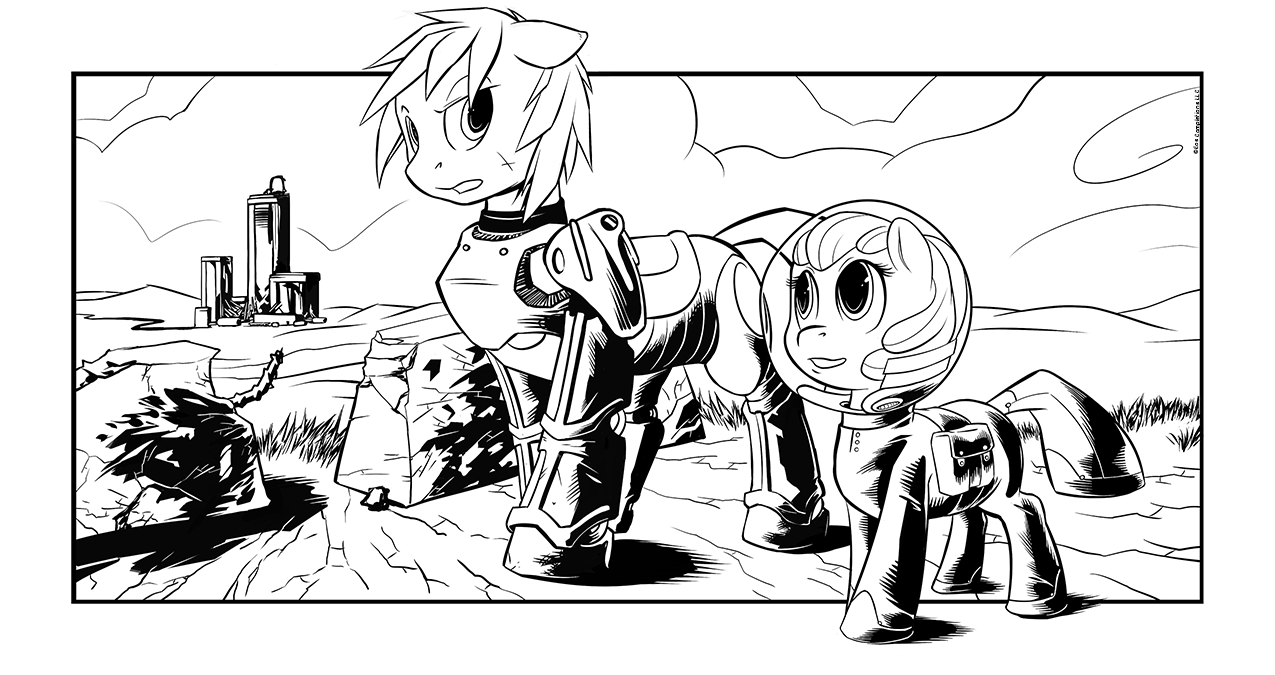
\includegraphics[width=0.9\linewidth]{image13.png}

\begin{intro}
I wanna know, have you ever seen the rain?
\end{intro}


\englishdaytimeplace{11}{18:00 P.M.}{Ivory Tower, Big 52 SC Branch}

Ivory Tower was a complex of large, white structures protected by reinforced ceramite plates. Before the war, the tower had been a research and development facility, where the Ministries of Morale and Peace worked together to find non-war oriented uses for the technological breakthroughs of the ministries of Arcane Science and Wartime Technology.

Nowadays, Ivory Tower was the only settlement on the Big 52 controlled by the Steel Rangers, mostly because it was the only place where you could find technology that hadn't been produced by Solaris Inc. And nopony with half a brain wanted to be near something made by Solaris Inc.

Yes, Solaris Inc., the company that merged a radio and a vacuum cleaner, creating the first sonic weapon ever, and putting it in the hooves of a very confused housemaid. They also invented a doorbell that incorporated a thief detection and disposal talisman, successfully electrocuting more than sixty door-to-door salesponies and a whole platoon of filly scouts selling muffins.

The central area of white buildings was surrounded by a moat and a perimeter fence, defended with automatic turrets and minefields. For more than a century, the tower held against every sort of invader, from raiders to organized war bands. Today the defenses were looking rather sorry for themselves. The turrets were destroyed and the minefields depleted. Even the perimeter fence had sustained heavy damage, having been cut in several places. The moat was crossed by two bridges, on the north and west sides of the complex, where two small collections of shacks were located. They were mostly warehouses for the caravans, and places where the traveling ponies could stay for the night and conduct business with the rangers with a roof above their heads.

The northern settlement had been almost completely razed, and the debris was used to build a barricade on the wasteland side of the north bridge, while the western group of buildings, which had been built around a couple of pre-war structures, had been hastily fortified and featured a pole with the flapping banner of the Applejack's Rangers.

The little fort was guarded by a dozen ponies, some of them still in their teens and wearing light combat saddles. A couple of fully fledged Steel Rangers in their standard power armor were guarding the bridge itself, while a third was patrolling the rocky area surrounding Ivory Tower, followed by a couple of recruits. A fourth ranger was inside the headquarters, arguing with a young mercenary.

``Yeah I can do that, no problem at all, but I want half the caps now, and some plasma stuff.'' Henrietta stretched her arms and reclined in the chair, putting her feet on the old desk.

The Ranger paladin cocked her head, a horrified expression on her muzzle. ``What do I look like, a garage sale? I'll give you a power lance, and that's already worth a fortune, but only when you're finished with the work.''

Henrietta snickered and shook her head. ``I'm a gunslinger. Don't offer me your fancy melee stuff. Three plasma grenades, two now and one later. Toss in a couple EMP mines and I'm your griffon.''

``Two EMP grenades now, a plasma grenade and a plasma mine later, last offer.'' The pony stretched her hoof towards the griffon.

Henrietta shrugged and shook the pony's leg. ``Deal. And half the caps now.''

``So you can fly away with them? I don't think so. You won't need them until you're done in any case.''

She sighed. ``You know what I think? I don't even think you have the caps. You hope that I'll accept and do the work for you, so that you can try an assault on the fort and then pay me with the caps that are inside the base. I don't think I want to play this game on the hope that four rangers and fifteen recruits will succeed in an assault against half a dozen better trained and heavily equipped ponies backed by sentries, and behind a solid defensive position.''

The paladin raised her hoof. ``All right, all right, you damn bloodwing, half the caps now! But don't expect any gratitude.''

Henri shrugged again. ``Gratitude doesn't buy bullets. I guess we have a deal. I'll be moving very soon, so be sure that your guys don't screw up.''

``All right, when you're finished, come back here and talk with Scribe Mellon. If you want to participate in the assault, I could have a little extra for you. Maybe some scavenged equipment.''

Henrietta was about to reply, when the pony in front of her held up a hoof, asking her to wait a moment. The conversation was interrupted by an emergency call for the Steel Ranger paladin.

``Cold Shower copying, report.'' The pony lowered her voice, but griffons have good hearing.

Henrietta sat in front of the desk, yawning. This wasn't her business, and she could drift away already, waiting for the night, but that thing about getting scavenged weapons from dead Steel Rangers seemed too good to be true. These ponies had to be really desperate if they made an offer like that to a griffon.

``Repeat that last part, please? You shot it dead how many times?'' The paladin's voice betrayed her disbelief. ``I don't think you can kill something more than once, Gauss.''

Henri couldn't help but turn her head toward the pony talking in the helmet, but Cold Shower was now ignoring the mercenary, immersed in her new conversation. ``What exactly do you mean by that? Are you at least sure that it's hostile?'' She paused, listening for a moment. ``So, basically, you shot it because it was creepy and it didn't even return fire?''

Henri jumped to her feet in alarm. ``Hey! Tell your guys to stop teasing Puppy!''



\horizonline

\englishdaytimeplace{11}{18:30 P.M.}{Ivory Tower, Big 52 SC Branch}

Puppysmiles trotted up to the small fort, looking at the rusty barricades and the guards on the perches. ``Hi pretty ponies! I'm Puppysmiles! Have you seen my mom?''

The glares that Puppy received in response to her greeting were mostly those of weathered ponies, tired from days of restless guard duties and broken by the awareness that they were not fighting some raiders or slavers, but ponies that they had once thought of as brothers or teachers. No, she couldn't find benevolence among this herd.

Puppy shrugged and kept narrating her interesting story to her escort. ``So, when Robocolt was sent away by the mayor, he decided to save the city all the same, because, you know, Robocolt wasn't just a robot, he was also a super kind pony!'' As usual, she didn't notice the general mood, and was already showering the poor patrol with her personal idea of what a pony with metal armor should do. ``But at that point Mom found me watching the movie and she turned off the TV.'' She shrugged. ``Meh, I can't see why she doesn't want me to watch cool movies. I mean, Robocolt is the good one. It's so obvious that in the end he'll win!''

Paladin Gauss sighed in frustration from his open helmet. ``Yes, sure, but I am NOT this Robocolt you're talking about! I'm an Applejack Ranger! It's different.''

Puppy giggled. ``You're funny, mister Not-Robocolt, I like you!''

``Yeah, whatever. Please, at least put away that dead parador! It's disgusting!'' Puppy had her pet sitting on her back. If the average pony would fear and hate such a dangerous predator, nopony could feel anything other than pity for that poor puny creature who was missing half its legs and a wing. Still, Puppy treated it like a treasure. Eww.

Puppy frowned. ``But Fuzzy Ball wants to see the pretty ponies! She will behave, I swear!''

The paladin facehoofed. ``I'm sure she will behave, but, uh, there are pet eaters around. It could be dangerous.'' He felt guilty, trying to sell her such an evident lie.

``Pet eaters? Where? Oh no, Fuzzy's in danger!'' She put the carcass of the little parador inside her saddlebags and started scouting the area in concern. ``Stay inside the bag, I'll take care of them!''

Gauss's jaw fell. He was trying to say something when one of the acolytes who had been accompanying them started laughing like an idiot, followed by the other two. Puppy stared at the laughing trio, seemingly clueless of what was going on. ``Ahahah! Very funny!'' Evidently, she didn't suspect anything.

Gauss looked away, trying to be as serious as possible. ``Right, you can never be cautious enough with those pet eaters around. Now follow me to our leader. And you three! Stop laughing like foals and report for duty at the front gates!'' He trotted away from the small group of acolytes, followed by Puppy.

``Okie dokie, Not-Robocolt! When are we going to fight crime?''

``For the last time, my name is Gauss! Paladin Gauss!'' He sighed. ``This is why I hope I'll never have foals.''

The duo finally arrived at the HQ, and Gauss opened the door, letting Puppy in before following her. The building was once a school, but now it was mostly collapsed, and all that was left were a couple of rooms and corridors that ended in a small office with white walls and a single desk in the middle. Sitting at the desk was another pony with metal armor and Henrietta.

``Henri!'' Puppy launched herself through the room, charging Henri, who effortlessly dodged the hug and caught Puppysmiles just behind the neck. Puppy struggled for a moment, trying to locate her friend. ``Hey! Where are you?''

``See? I told you that we were going to meet again.'' She put Puppy down and patted her on the helmet, snickering. ''So, Paladin, this is a friend of mine. Can you keep an eye on her while I'm doing my job?''

Cold Shower tilted her head while looking puzzled at Puppy. ``This pony was shot four times, and not only does she show no sign of it, but she's also in a good mood. I don't think I should accept her in this place until I know what I'm looking at. Gauss, call Scribe Scold.''

Puppy didn't care very much about the paladins. Now she had Henri, and this was way better. ``Yup! Mom is somewhere in the white houses on the other side of the bridge! I was going there, and I met these pretty ponies and mister Not-Robocolt!'' She finally succeeded in hugging her target. ``I'm so happy to see you again! Tell me you won't leave me alone this time!''

Henrietta cleared her voice, looking away from her. ``Uh, actually, I have a couple of things to do, but I'll be back if you wait here for me. It won't take long.''

Puppy frowned for a moment, asking uncertainly, ``Ah, will you take Silky Tail with you?''

``Sickly who? Oh, the doll! Yeah, sure, why not?''

She sighed in relief. ``Then it's all right. Just let her help you, she's good.''

Henri patted Puppy on her helmet. ``Cool, now stay with the rangers and behave. Don't make them mad, and don't run away. When I'm back I'll let you hang with me, all right?''

``Yush!'' Puppy waved goodbye to Henri as she left the room.



\horizonline

\englishdaytimeplace{11}{19:00 P.M.}{Ivory Tower, Big 52 SC Branch}

Scribe Scold was an old pony who had trained many acolytes over the years, and his cruelty and coldness toward everypony made him infamous among the young recruits. There was only one way to gain the old scribe's respect, and that was by doing a perfect job every time. When he turned against the Steel Rangers, joining the Applejack's Rangers, everypony had been surprised by his choice. In fact, a lot of the defects still thought that he was a spy.

Scold approached Puppy and looked into her eyes while talking with Paladin Cold Shower. ``Canterlot ghouls have the same scars as usual ghouls, so I don't think she's one of them.''

Cold Shower sighed, sitting behind her desk. ``Then what could this foal be? She survived four direct hits. One in the head, and three in the heart.''

``Can I has a red cape too?'' With these words Puppy grabbed Scold's cape and looked at it in amazement. ``I like the golden thingies! Gold is Pretty Princess Celestia's color! When I'm a big pony I want to be a princess too, but I need the gold! Please?''

``Runes. They're runes, and you can't \emph{have} it. Now sit down and behave.'' Scold turned back to Cold Shower. ``It could be something necromantic, I'm almost sure of that. If we had access to the library I could do some research, but at the moment I can only guess.''

``Why I can't has, ah, have it? I can give you something in exchange. It's a \emph{barter}! It's cool! Big ponies do barters every time and it's okay, not like when I changed my breakfast for two marbles and then I was really hungry and Mom scolded me! This is okay!''

Cold Shower nodded, trying to ignore Puppysmiles. ``So, what's your guess?''

Scold gave a stern look at Puppy. ``No, I don't intend to barter my cape with you. Now behave and wait until the 'big ponies' are done talking.'' He sighed before going back to Cold Shower. ``I remember reading something about these radsuits. They were less than effective during the Canterlot attack, and almost every foal wearing them was turned into a ghoul.'' Scold paused for a moment, looking at Puppy still trying to pull off his cape. ``Not this one, I'd say. Maybe I should run a diagnostic test on the suit to see what comes out.''

Scold connected his PipBuck to the data socket of Puppy's suit, keeping her still with the other leg. ``Now please stay still for a couple of minutes.''

``Can I hug you? You are funny, I like you!'' Puppy paused for a moment, pondering. ``And I like your cape, did I say that?''
>
Cold Shower couldn't help but chuckle, despite the situation. This won a grim glare from Scold. ``Yes, you can hug me as long as you stay still. Now, let's see what we have here.'' He frowned. ``It says she's deceased. No heartbeat, no body temperature. Actually, no body at all, just two thousand bone fragments and about one hundred and eighty grams of organic matter. No, it's definitely not a ghoul.''

``Tee-hee, Red Cape talks funny!''

``Yeah, Scold, stop talking funny and give me a version for the troops. Since you rejected my application as a scribe I'm more into guns than scholarship.'' There was no bad blood in Cold's words, but he occasionally needed somepony to remind him that he wasn't in his classroom.

``I still don't know. I can only say what she isn't.'' Scold looked back down at his PipBuck, reading the results of his analysis. ``The artificial intelligence of this suit is intact and working perfectly, so I'm pretty sure this is not a crazed robot. Oh, look at this. The main healing talisman failed two hundred years ago, during a reboot. A one in a thousand chance, probably caused by a short circuit or a flawed component. This activated the backup talisman.''

Cold Shower raised an eyebrow. ``And why this should be interesting?''

He snickered. ``Because the backup healing talisman had a different function to the main healing talisman.''

Cold snorted. ``Yeah, give me your information a bit at a time. Do you want to finish this thing or we are going to wait for the morning?''

Scold sighed, ignoring her comment. ``This thing doesn't seem to contain a single healing spell, just a program to manage and inoculate potions from the suit's stash. No wait, there's something else, but I don't recognize the matrix, it uses\dots zebra runes? What the hay could zebra runes be doing inside a healing talisman?''

Cold sighed and muttered, ``They could, uh, save one hundred and eighty grams of organic matter?''

He kept working with his PipBuck. ``Yes, a partially decomposed heart, I'd say. This is interesting. Scanning the inside of the suit I can see a couple of deformed high caliber bullets floating in the heart's proximity, as if they hit it without damaging the organ.'' Scold pondered for a moment. ``Let's see if I can access the registry of that talisman, then I could see how it was supposed to work.''

All this talking was plain boring. Puppy was a notoriously patient filly, but not even the most patient pony in Equestria would've been able to stand all that blah blah blah. So, she put her hooves in the scribe's pockets and started browsing through his possessions. She found a quill, some paper, a book, a pair of glasses---SNAP---uh, a monocle, another monocle. ``Hey, what's this?''

Puppy took a brushable plastic pony out of Scold's pocket. It was a green and white unicorn with a broad smile and a lyre as a cutie mark. ``D'aaw, it's so cute!'' She started petting the doll's mane. ``Brushie brushie brushie. Brushie bru---''

``What the---hey, give her back!'' He snapped the doll from Puppy's hooves, putting it back in his pocket. ``Play with your own dolls. This is an action figure, and it's very delicate and---'' Scold's eyes met Cold Shower's, and he realized what just happened. ``No, oh no, no, no no no! It's---it's a toy I confiscated from an acolyte! It's not mine!''

Puppy's eyes widened as soon as she heard that the doll hadn't a proprietor. ``Not yours? I can has that then! I'll love her and pet her and have tea with her and we will always play together and we will be best friends forever! I'm calling her Bonbon and I'll make her mane pink!''

Scold's composure evaporated when he heard about dying the doll's mane. ``Her name is Lyra and you can't HAS it! It's MI---ehr, it's confiscated material and needs to be scheduled and classified!''

An amused, evil grin appeared on Cold Shower's muzzle as she walked around the desk and trotted toward the duo. ``Oh, don't be so strict, Scribe Scold, I'm sure that we can let a little filly play with a foal's toy, right?'' Cold Shower was smiling widely, but she would have needed even more teeth to really show just how much fun she was having right now.

``See? See? Robocolt says I can has it! Gimme gimme gimme!'' She tried to pick Scold's doll again from his pockets, but this time he was on edge and blocked her.

``It's mine, okay? Lyra is mine! I can't give her to you because I like her! Are you happy now? You, ah---'' His expression changed while he looked at Cold Shower. After all, safety in mutual destruction could be an option. ``You can have a toy from the paladin's room if you wish. She will be very happy to let you rummage in her quarters, because I am sure she has nothing embarrassing to hide. Am I right, Paladin Robocolt?''

Shower's smile died as she quickly coughed and looked away. ``Ah, I'm sure we'll find some pretty toy for you, little one. Now, uh, please behave and stay put while the scribe finishes his work, okay?''

Puppy smiled in glee. A promise of new toys was good enough for her to let this funny pony with the red cloak mess with her space suit for as long as he wanted. ``Okie dokie!''

Scold sighed and launched one last accusing glare at Cold. ``Could you please stop grinning like that? I'm trying to focus here.'' He went back to his instruments, mumbling. ``Oh please, you're kidding me. They couldn't include such a feature in a healing talisman!''

Cold Shower looked puzzledly at Scold. ``What did you find? Is it as bad as it seems from your face?''

``I-I'd say it's worse. Somepony at the Ministry of Peace went to extreme lengths to make sure that these foals didn't die; that they weren't \emph{allowed} to die.''

``Weren't allowed? What do you mean by weren't allowed?'' She raised an eyebrow.

``I mean that the last resort of the backup talisman consisted of some sort of \emph{necromantic} spell. I'm not sure how it works, but it seems to bind the life of the patient to what's left of her.'' He sighed. ``Luckily enough, it doesn't seem too powerful a spell. I think it could be undone, but it will take a lot of time and study. Moreover it will require way more magical power than just my own. And I need my library.''

Cold Shower whistled. ``Talk about tough love. How could somepony do something like, like forbidding you to die? How is that even possible?'' she objected.

``Since we are facing it, I'd say it is. I'm not an expert of necromancy myself, but I can tell that the talisman itself isn't in great condition. It stayed active for two hundred years with just a single spark of energy. I can't explain it. This shouldn't work at all! There must be something else, an external factor, maybe.''

Cold tilted her head. ``So, basically, the foal is some sort of ghost?''

Scold tapped his chin. ``I'm not sure. I need to study this phenomenon a little longer. I think that the talisman somehow linked everything together. The suit, the pink goo inside it, and the remnants of the foal's body. A ghost? I don't think so, but I can't say. Technically, this poor creature shouldn't even be capable of walking around. Its magic isn't strong enough. Instead she behaves like a foal, has memories, and acts as if everything about her was normal.''

He paused for a moment, rubbing his eyes. ``Looking at this log. The suit went almost dead and didn't move at all for two centuries. Then all of a sudden its batteries got charged way above their maximum capacity, and every spell inside the suit began working at five times its effective potential. I can't explain this with science or magic. Maybe she's a ponygeist?'' With a very tired expression on his muzzle, Scold snickered and let go of Puppy's hoof. ``All right, we're finished here, little one.''

Puppy smiled back at the scribe and replied, ``Yay, now I have to go and find my mom, but I'll be back for the toys! Bye bye!''



\horizonline

\englishdaytimeplace{11}{19:45 P.M.}{Ivory Tower, Big 52 SC Branch}

Puppy pouted, looking at the closed door. ``But I have to go find my mom! I can't stay here!'' She banged at the door, but nopony answered her. She was trapped inside the classroom.

Those stoopid Robocolts put her in a room, luring her with the promise of toys, and now she was sitting in some sort of kindergarten, prisoner of those meanie ponies. Well, they actually gave her some dolls and a lot of crayons, and even a super nice coloring book, but she had no time for this! She had to find her---``Oh look, this picture has butterflies!'' No, Puppy! You must resist! You have\dots to find\dots ``Woah, a golden crayon! It's actually the color of gold! I can color Pretty Princess Celestia with this, and she will be super identical to the real one!''

No! Mom comes first! Puppy was a filly on a mission! She put down the super cool crayons and looked away. These fancy things won't keep her down! Never! ``Is that\dots a \emph{real} teapot, with \emph{real} tea cups?'' Puppy lost her battle.

Not even five minutes later, the situation was critical again. ``\emph{GASP!} Miss Fuzzy Ball ruined Rarity's gala dress, and if they don't find a gold crayon the whole gala will be spoiled! But look! Here comes Pretty Princess Celestia with a gold crayon! And there's Rainbow Dash, too! The gala is saved, yay! Now it's time to celebrate with a good cup of tea!'' Puppy was moving the dead parador and some other dolls around, talking to herself with a very focused expression on her muzzle. It was clear that she couldn't be distracted, since the gala was completely depending on that tea party.

Scold moved away from the window, shrugging. ``It seems that she won't be a problem. Keep a couple of acolytes at the door, just in case something happens, and get back to tonight's assault preparations.''

Cold Shower shivered, following the scribe. ``She seems so\dots oblivious. What should we do with her? It doesn't seem right to keep her prisoner like that, and sooner or later she will try to go and find her mother again.''

Scold sighed. ``I think I can dispel her curse. The spell is weak enough, but I must study the ritual, and I'll need other unicorns.''

``But, will she die?'' The concern in Cold's voice was evident.

Scold replied slowly, talking deliberately as if he tried to explain a very easy but vital concept to a simple mind. ``She's already dead, Cold. That little pony deserves her eternal rest. She shouldn't even exist.''

``But, she doesn't seem to care. We could at least try to see if her mother is still alive. Maybe she's a ghoul! If she lived here, there could be some information about her in the library.''

He shrugged. ``Which brings us back to our original problem: getting back my library. So, put a couple of acolytes guarding the room and start the preparations for tonight. When I have the instruments, we will discuss how to solve this problem.''



\horizonline

\englishdaytimeplace{11}{22:00 P.M.}{Ivory Tower, Big 52 SC Branch}

A little more pink in the clouds, aaand\dots done! Puppysmiles looked amazed at her new creation. Who said that you couldn't paint a picture using only pink? Pink went with everything! Now, she just needed to stick it to the wall with the others---\emph{BOOM!}

The windows shook, and for a moment there was a big red flash outside, making Puppy turn on her tail and stare in curiosity. ``Fireworks?''

\emph{BOOM!}

Another red light flared outside, and a window shattered, launching glass shards all around the room. Sharp window fragments rained on the floor, on the desks, and against Puppy's helmet. She didn't care. Instead, she stuck her head outside to get a better look at whatever was happening.

``Yay, fireworks!'' Lucky Puppy, this was a great show! Past the bridge, on the other side of the moat, a lot of ponies were running and playing, throwing fireworks and a lot of other noisy and colored lights to each other. For sure, these robocolts knew how to party hard, and Puppy wanted her share of fun.

She headed for the door, but she remembered that it was closed. Obviously this didn't discourage Puppy. She simply jumped through the window.

Landing on the road outside, Puppy hesitated. Leaving behind all those toys and pretty drawings was not easy, but everypony has to make sacrifices in order to follow their goals. What did Soft Air say? One day she would have to make sacrifices and find that not everything was easy, and you have to leave something of yours behind if you want to go on. Puppy now knew that the ugly pony was right, and Trigger Happy too, but she was a filly on a mission, and she wanted to see the fireworks from closer, so, goodbye, pretty toys. Oh, and she still had to find Mom! Finding Mom was important, too! Go Puppy!



\horizonline

\englishdaytimeplace{11}{22:15 P.M.}{Ivory Tower, Big 52 SC Branch}

The whole area between the bridge and the main research building entrance had become a battlefield. The four Applejack Rangers were supporting the attack with their heavy weapons, but the real assault was performed by the acolytes, protected only by light armor, and armed with light caliber weapons like assault rifles and submachine guns. When Puppy crossed the bridge, Paladin Gauss didn't notice her immediately and she slipped past him before he could react.

``Fuck, what is she doing here? Shower, the ghost is on the field!'' He tried following Puppy, but he had to dive behind cover again when a barrage of bullets hit his position. ``No can do! If I move I'm dead! Moreover, group two needs cover!''

Puppy noticed a young mare lying beside a smoking crater. As she approached, she could see that a pool of red had formed beneath the sleepy pony and that it was continuing to grow. ``Hey, is something wrong pretty pony?'' Puppy poked the acolyte, who weakly opened an eye.

``P-please\dots Help me\dots I\dots I don't want to die\dots'' The soldier's voice was feeble, and she couldn't even move.

Puppy gently patted the acolyte's mane. ``Don't worry, fireworks can be a little scary, but you are a big pony, so you don't have to cry.''

The dying pony stared up at her blankly, not even hearing the foal's comforting words. ``I\dots don't want to\dots die\dots'' She was a young mare, probably a fresh recruit at her first and last battle.

``There, there.'' Puppy sat down next to the pony, continuing to stroke her mane. ``I'm here, don't worry, there's nothing to be scared of. When the fireworks end we will go and buy cotton candy, okie dokie?'' The first time Puppy saw fireworks she was scared too, but Mom bought her cotton candy and she stopped crying. It must have worked with this pony, because she stopped whimpering and now she was simply crying. A couple of bullets hit Puppy in the torso while she sat beside the mare, but she hardly noticed.

``Mom\dots Sorry\dots Why I\dots ran away?'' The acolyte's dying words were barely a whisper as her last breath left her lips.

``Uh, don't worry miss pretty pony, moms are good and nice. She will be happy to see you again even if you ran away. Ah, maybe she will scold you, but I'm sure she cares.'' The dead pony didn't reply, so Puppy tried poking her. ``Ah, are you all right? Miss pretty pony? Ah, Mister Voice, is this pony all right?''

{\mt ``Analyzing. Negative. Applejack Rangers Acolyte condition: deceased.''}

Puppy frowned. ``Oh, like Henri's dad.'' Finally, Puppy seemed to catch up with the situation. ``Hey, Mister Voice, are these ponies playing or fighting?''

{\mt ``The ponies in the area are fighting, though none of them are marked as hostile toward you. Only point defenses are marked as enemies.''}

To reinforce the suit's words, another couple of bullets hit near Puppy's position, and one partially cracked her helmet.

{\mt ``Warning. Breach in the containment layer. Repair talisman activated. Hostile count: two.''}

``Hey! Look where you point those things!'' Puppy stood on her hooves, leaving the dead pony and trotting toward the nearest group of acolytes who had found shelter behind an upturned cart. ``Stop fighting! It's dangerous! Your friend is very ill!''

One of the three soldiers stared at Puppy. ``What the fuck are you doing here, filly? Find some cover!''

She tilted her head, confused. ``Why?'' Exactly at that moment, a spray of bullets hit Puppy's flank, leaving a thin trail of pink when the bullets pierced her body as if she had been made of butter.

The acolytes stared at the scene in horror, but when Puppy simply yelled at the turret to stop being a bully, they seemed speechless. The trio of soldiers didn't even react when she lost it and galloped toward the Steel Ranger's most advanced defensive position.

``Stop that! It's dangerous, stoopid bullies! Can't you see that everypony is scared here?'' Puppy charged directly toward the main building entrance, where a couple of Steel Rangers were shooting at the assailing forces.

One of the rangers turned toward her and shot at her with grenade launcher, sending her flying over to the other side of the battlefield. Puppy took a minute to recover from the explosion, and in the meantime Paladin Cold Shower managed to reach her.

``What the hay are you doing here, Puppy? Go back in the school building!''

Puppy sat down, shaking her head. ``Nope, I don't like ponies arguing with each other. Ponies should be pretty and nice, not mean and violent!''

Cold cocked her head. ``This is war, Puppy! You can't stop it by just whining! We'll handle this one. Don't worry and run back to the school. It's too dangerous here!''

``Ah! There is no war that Space Captain Andromeda can't stop!'' She lifted one hoof and stated, ``Lazer Gun!'' Sentenza floated in front of her.

Shower tried grabbing Puppy, but a burst of bullets forced her to get back into cover. ``Put away that toy gun and come with me! Puppy! Are you listening to me? Puppy!''

She galloped into the middle of the battlefield, grabbing the gun with both her hooves and pointing it at the ponies defending the main building entrance. ``Stop fighting and surrender or I'll shoot! You are bad ponies, and you should feel bad!''

A turret hit Puppy in a leg and in the belly while the rangers ignored them. Cold Shower desperately looked for an opening in the barrage of fire to dart in and grab her.

``Okie. Dokie. Lokie. Space Captain Andromeda, to the stars and beyond!'' She dived onto the ground as if she was dodging invisible laser rays and pointed her own ``toy'' gun, before stating a single word.

``Bang!''

Half a dozen times.

``Bang! Bang! Bang bang! Bang! Surrender nao, stoopid zebra aliens!''

{\mt ``Target one to seven acquired. Opening communication bridge to Ponymedes through Comm Station two. Ponymedes status: restored and functional. Relaying coordinates.''}

A window on the third story of the central building exploded from the inside, and a griffon flew out of it, firing a pistol back into the room she just left. The griffon's appearance on the battlefield completely gained Puppy's attention.

{\mt ``Ponymedes I, IV, V, IX, X and XII are ready to fire. Ponymedes II, III, VI, VII and VIII have target beyond their horizon. Relocating for indirect fire. Estimate time: 30 seconds.''}

``Henri! HEEENRIII! I'm here! Make these ponies stop fighting please! HEY! HENRI!'' Puppy tried to gallop after Henri, with Sentenza still in one hoof and a turret stubbornly firing at her. ``WAAAAAIT!''

Stoopid chicken, that girl always needed some help to notice things! Puppy put away the gun and took a chunk of asphalt from the ground, taking aim aaand---bull's eye! Henri lost control of her trajectory and landed, well, crashed, not far away from Puppy.

In the darkness of night, Ponymedes opened its eyes. Half a dozen red lights pointed at the roof of the base's main building. At first they were only pale, thin, crimson lines moving randomly in the area, but they grew in intensity until you could see them even from the other side of the bridge. Like red laser beams, they appeared from the clouds, piercing the gray curtain and coloring it with faint red shadows, seven small pillars of light connecting Ivory Tower with the heavens, and beyond.

``EVACUATE THE AREA! ALL PONIES LEAVE YOUR POSITION AND RETREAT!'' Enhanced with magic, Scold's voice thundered above the explosions. Every acolyte began falling back, following Scold's order, leaving their cover and running toward the bridge. The rangers defending the central building seemed confused, and held their fire as they watched the retreating forces.

``Fuck, Puppy, why did you throw a stone at me this time?'' Henrietta was rubbing her head, still trying to work out what was happening. ``What's the old mummy screaming?''

Puppy shrugged and hugged her friend. ``Dunno, but I wanted you to tell them to stop being mean, only it seems that they are already stopping.''

{\mt ``All weapons ready to fire. Target is locked. Commencing full scale attack in ten\dots nine\dots''}

\clearpage % must clearpage

~\vfill

\begin{engnote}
		Level up! (12)
	
		New perk added: Little Scoundrel - No Puppy, give it back! You are less likely to get caught when stealing, in addition you can access to NPC's inventory during dialogues if you are facing them.
\end{engnote}



\chapter{Rag Doll}

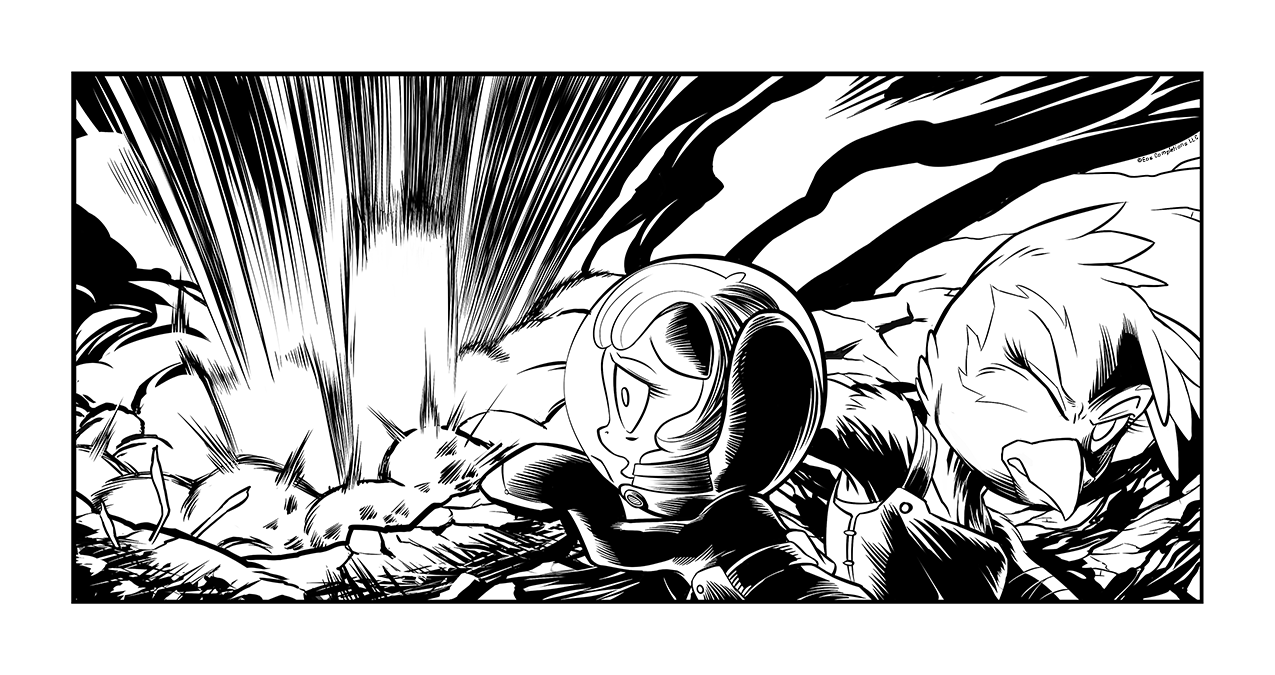
\includegraphics[width=0.9\linewidth]{image14.png}

\begin{intro}
Into each life some rain must fall\dots
\end{intro}


\englishdaytimeplace{11}{22:30 P.M.}{Low orbit, $\approx \SI{1800}{km}$ above Equestria}

High above the planet floated Ponymedes I, a giant of plastic and super light alloys that had a body shaped like a large sunflower and long solar panels that formed its petals. There were words and signs painted across the satellite that warned against a multitude of dangers, such as fire or falling rocks, but the only one that held some meaning for an observer was the Solaris logo, with its male alicorn and the company motto ``Try the alternative'' encircling the image.

Attached to the satellite's large round body there were four barrels, easily longer than a couple train cars. The weapons were composed of two linear metal rails held together by many rings, placed only a few centimeters apart from each other. It functioned as a weapon that use a sequence of strong, magnetic pulses, and a potent electric thrust to propel a metallic body at unpony speed against very distant targets. In other words, it was a deadly weapon, and Ponymedes I was armed with four of those little toys.

But at Solaris, nopony left a work half-baked. How could a single satellite always be ready for action? They needed a network of satellites, a complete shield ready to defend Equestria or whomever made a better offer for that little jewel. Ponymedes had eleven siblings, able to change their distance from the planet and move around in orbit to operate in groups. Now the whole family had been reunited, and each of the twelve brothers had their guidance lasers pointed at their own designated target.

{\mt ``\dots Eight\dots seven\dots six\dots''}

As one, the four barrels began to discharge sparks of blue electricity from between each ring and all along the metal rails as the the countdown steadily ticked away. A metallic bar coated in ceramics, more or less one and a half meters long, and shaped like a pointy stick, was placed into the barrel by an automated loading system and immediately enveloped by a blue halo.

{\mt ``\dots Five\dots four\dots three\dots''}

Behind the satellite, four hatches opened to reveal the exhaust vents for the recoil compensation system, a dim red light appeared inside each of them, glowing like lava within the belly of a volcano. All four barrels were now completely blue, powered by the electricity running from ring to ring. They resembled four bright lances, ready to unleash their fury against a doomed opponent.

{\mt ``\dots Two\dots one\dots''}

{\mt Fire.}



\horizonline

\englishdaytimeplace{11}{22:30 P.M.}{Ivory Tower, Big 52 SC Branch}

{\mt ``Attack commenced. Estimated time of arrival for the first salvo: seven minutes.''}

Half of the guidance lasers disappeared, and a couple shifted kilometers away in the blink of an eye, as if something up in the heavens had gone awfully wrong. Still, five red lights continued to shine down on the building's roof, flickering once or twice, but staying on target.

``Why is everyone retreating now?'' Henrietta opened her wings, ready to grab Puppy and fly away with her.

Puppy pointed at the besieged building entrance. ``Those two aren't running away, we can ask them!'' And with these words she tried to trot towards the two perplexed paladins defending the main research building.

``I don't think so! My job is done here, and we're following the example of our fleeing friends.''

``TO ALL THE PONIES INSIDE THE BUILDING! YOU ARE BEING ATTACKED FROM THE SKY! EVACUATE THE FORT! WE CALL FOR A TRUCE! RUN FOR YOUR LIVES!'' Once again, Scold's voice thundered above the battlefield before he turned on his tail and ran, following the acolytes and the other scribes.

Finally, Henri looked up at the clouds, and her beak hung open as she saw the red lasers cutting through the darkness of the night. ``Oh, rotten eggs. If those are what it uses to aim, I don't want to see what it fires!''

{\mt ``Warning. Lost signal from Ponymedes III, V, X, XI and XII. Ponymedes IV and VII report major failures with the recoil compensation system. Ponymedes I, II, VI, VIII and IX are commencing the second barrage in ten\dots nine\dots''}

Puppy frowned. Mr. Voice had been talking for a while now, and it didn't seem like he was going to stop any time soon. Everything was becoming really confusing. Why was everypony running away? Why was Mr. Red Cape yelling so loud, and why was her helmet showing her all these blinking red lights everywhere? ``How do I make all this mess stop?''

``I don't know. I don't care! Let's get out of here!'' Henri took flight, grabbing Puppy and gaining height and speed with each stroke of her eagle wings.

Okay, new problem. Flying. Puppy had thought up a plan for the next time she had to fly, something she really, really had to do. What was that already? Oh, right, scream. ``EEEEEEP! NONONONONO!''

``Shut that trap! I'm trying to save your life!'' After her running start, Henri began to lose speed and altitude, dragged down by Puppy's weight. ``What the fuck are you carrying around now? I made you throw away a ton of junk, and you're already full of useless stuff again! Aargh! Unload the bags or we'll crash!''

{\mt ``\dots two\dots one\dots Second salvo out. Readying guns for third salvo.''}

``LEMME GO! LEMME GOOO!'' Puppy was struggling, in the middle of her personal world of things moving too fast and too far from her hooves to be comfortable with.

Henrietta tried cutting one of her saddlebags with a talon, slashing desperately at the bottom of the container, and missing it several times before finally managing to hit the moving target. ``Gotcha!''

{\mt ``Repair spell activated. Lost signal from Ponymedes I and II. Ponymedes VI, VII and XI will be ready to fire in ten\dots nine\dots''}

The hole in the bag closed almost immediately, while the inventory management spell kept everything in its place.

``Hey, that's cheating! Do you want to play rough? I'm in!'' She let go of Puppy from one side, turning her upside down. This strategy worked a little better because one of the bags wasn't closed. Puppy rapidly lost weight as she left behind a trail of odds and ends in the sky: empty bottles, roasted plushies, and a small toy cart.

``NONONO! I'm gonna pee myseeeeelf! Please stop! PLEASE!'' Puppy was completely terrorized by the situation, and being dangled in the sky like that only made things worse. She succeeded in grabbing The Rock Of Destiny as it fell from her bag, although a lot of the cool stuff she found was lost forever. Everything was going bad today, and she didn't even have time to complain, since stoopid chicken Henri was teasing her hard. ``You bully, let me go or I'm telling Mom!''

When Puppy had finally reached a bearable weight, Henri lifted Puppy onto her back, hoping that that would lessen the screams. ``All right, all right! We're done, now be quiet and I'll put you down when we pass that hill!'' Henri had no idea of what was going to rain down from the sky, but her life as a mercenary had taught her the value of cover. Actually, she wondered why nothing had happened yet, but she suspected that the longer whatever it was took to arrive, the worse it was going to be. ``We can't land here, Puppy! Try not thinking about it. Listen to some music and close your eyes!''

Puppy was barely listening, but the music idea suddenly seemed like the best idea ever. ``Music! Now, please!''

The radio came to life, while on the ground ponies ran as fast as they could. Both the Applejack's Rangers and the Steel Rangers who had decided to believe the old scribe were now running for the hills.

\rtpr{``Hello fillies and gentlecolts! Isn't it well past your bedtime? This is Lonesome Pony, and you are listening to Radio 52, the only radio that brings you news and safety, from the Ridges to Emerald Shores! Tonight we have a lot of things to talk about, so let's get to business.''}

Not music. Why was it that every time Puppy turned on the radio, the first thing she heard was the stoopid chatty pony? Puppy wanted some music! The ground was a rushing blur down below, and Mister Voice wouldn't stop chatting, and now even Lonesome Pony was giving her a lecture instead of some music? Puppy wanted to cry. In the background, the suit informed her that the surviving three satellites were continuing their attack.

\rtpr{``First things first, Things are getting messy along the South Branch. It seems that the Wild Herd is ambushing the patrols from Ironworks again, but this time they seem to be better equipped, and way more organized than in the past. Maybe they found a new leader? This could mean big, big trouble in the near future. Don't lower your guard if you are traveling south of Broccoli, or from the Memorial to Ironworks, and try avoiding the east route to Emerald Shores. Stay on the road and turn your tails as soon as you see something suspect. Better safe than sorry!''}

Henri soared through the air, easily surpassing the ponies that led the retreat. They were slow, too slow to get to a safe distance in time, but there was a good chance that even she and Puppy were condemned, so why not try running anyway? With a stroke of her wings, Henri gained speed and kept flying straight, despite the choking grip Puppy had around her neck.

\rtpr{``Now, since bad news never trots alone, we have a new change of policy from the NCA, rejoice! The NCA forces have decided that every trader is actually a raider, so they started arresting traders and confiscating the merchandise on their borders, yay! If you were planning for a trip there, you better reconsider and try heading for Salt Cube City or Tunnel Town for trading your goods, since the northern branch is now safe.''}

Henrietta landed behind the hill, panting heavily. Puppy jumped down from her back as soon as she could see solid ground and immediately stuck out her tongue at the big meanie chicken. ``Bleh! Why do you always bully me? I'm your friend!''

``Fuck off, Puppy.'' Replying with almost no breath in her lungs was quite hard for Henri, but Puppy couldn't have things her way every time. ``I'm not bullying you. Something is going to happen in that place, something bad.''

\rtpr{``And now the last news. It seems that an old merchant came back from his longest trail. He started four years ago with a cart full of garbage and a brahmin, and he's back with, well, a brahmin, a cart full of garbage, and a lot of stories! Maybe over the next day I'll tell you all about the places he visited, but it seems that those ponies in the far west are crazy! He told me about a city of lights, and great walls crossing a river, imprisoning it to produce energy. Woah, we could use something like that, couldn't we? And this ends the news. Have some good music, my little ponies!''}

Puppy cocked her head in surprise. ``Something bad? But Mom is there!'' Puppy turned towards Ivory Tower, now more than a couple kilometers away, illuminated by the dim red light of a single surviving laser beam. The clouds above the old research facility flashed with white light for a moment.

At which point the radio decided to start playing music.

\begin{music}
		Raindrops keep falling on my mane,
	
		And just like the foal whose cutie mark is not there,
	
		Nothing seems to fit there.
\end{music}

Blazing lines of white burst through the clouds. Like tiny silver darts shining in pure heat, they rained down from the heavens onto Ivory Tower. The magnetically accelerated shots crossed the cloudy sky in a split second, striking the buildings and the area nearby with such force that for a moment, Henri could have sworn that she felt the earth shudder beneath her feet.


\begin{music}
		Raindrops are falling on my mane. They keep falling---
\end{music}

First arrived the flash. A white halo rose from the impacted structure, then the walls seemed to expand for a moment, reminding Puppy of a balloon being inflated. For a short instant, everything seemed to hang in the air, as if time had stopped, leaving the building floating there, separated into its many elements. Walls, windows, doors, all like in one of those drawings that showed all the parts of a cart or a house that Mom had shown her that one time. That instant of stillness only lasted for the blink of an eye. Then everything flew away in different directions. Chunks of wall as large as trucks went flying through the sky like shreds of paper, surpassing even the moat and landing on the bridge and shacks beyond, making them crumble like a cardboard castle.

Then came the sound. The first thing Puppy heard was an acute whistle, like when you try making that weird music with grass leaves. But it didn't last for long, because immediately after it arrived the boom. Not just one big boom, but the sound of many thuds, followed by the booming thing. It was like a rapid fire concert, a thud then a boom, a thud and a boom, a thud-thud and a badaboom. Wow, catchy.

Puppy really wished that Mom could have been there to see that show. It was so fun! No wait, Mom was there. Actually, Mom was supposed to be inside that super nice white build---oh.

Her eyes widened as she lifted a hoof towards what was once Ivory tower, her expression becoming a mask of fear. ``Mom?''


\begin{music}
		So I just did me some talking with the sun,
	
		And I said I didn't like the way she got things done.
	
		She's sleeping on the job.
\end{music}

{\mt ``Warning. Ponymedes VI is out of ammunition. Signal lost from all the other satellites. Attack aborted. Area will be safe from incoming fire in fifteen minutes. Thank you for choosing Solaris Inc. as your main siege weapon system. Solaris: try the alternative.''}

Puppy stared unblinkingly at the white points of light as they continued to pierce the clouds and rain down like tiny stars on what was once her mission objective. Why didn't they stop? Wasn't that enough? They already made a lot of noise and stuff, so now it was time to stop, right? It's fun only if it lasts a bit, but then it becomes scary. Puppy held her breath, praying that every silver shard falling from the sky was the last, but they never seemed to stop. There were always others coming.

They were destroying the place where Mister Voice told her that Mom was. But wait! The arrow was still there! Yes! There was still hope! Puppy rejoiced. Nothing could stop Mom! Take that, stoopid silver rain!

\begin{music}
		Those raindrops are dropping on my mane. They keep falling---
\end{music}

Another hail of falling stars fell in the cloud of smoke and debris, this time hitting somewhere near the research center's power plant. It was easy to tell, because the thud was followed by a ball of green fire that exploded upwards towards the sky, producing a glowing mushroom cloud in the middle of the mayhem. Okay, that was new, and it was unfair.

{\mt ``Warning. Mild radiation detected. Threat level: negligible.''}

The pink arrow on the compass blinked three times and disappeared. Puppy waited for it to reappear, hoped for it to reappear, and begged for it to reappear, but the compass remained empty. The suit informed her that the mission 'Chasing Rain' had been completed.

Why were those silver things still falling even now? It was over, all over. The arrow was gone. Mom was gone! Mom\dots was gone? No, that couldn't be! Mom was\dots Mom was where the arrow said, but now, now the arrow didn't say anything! Puppy followed that arrow only because it pointed at Mom, and now there was nothing to follow! There was nothing left, just\dots just a bunch of falling stars and---and for the first time since she left Canterlot, she didn't know what to do.

Mom was gone.

\begin{music}
		But there's one thing I know.
	
		The blues they sent to meet me,
	
		Won't defeat me.
\end{music}

Puppy's right eye twitched. She stood still, eyes wide open and staring, her muzzle petrified in an expression of surprise. Henrietta put a paw on Puppy's shoulder, trying to say something in the deafening thunders of the bombardment. Whomever began that attack wanted to be double sure that nothing was left of the whole place. Even after the generator's explosion those white missiles kept arriving. These guys had ammo to waste.

``Don't worry! Your mom wasn't there! I was inside the place, she wasn't in Ivory Tower!'' Puppy didn't react. She probably didn't even hear her words, so Henri tried shaking her, but the pony didn't offer any resistance, simply moving like a rag doll, her blonde head bobbing inside the helmet.

\begin{music}
		It won't be long till happiness steps up to greet me.
\end{music}

``Oh, c'mon, Puppy! You have been through things way worse than this! Hey, I'm talking to you!'' Henrietta poked Puppy again, making her head bob a little more. ``What the fuck? Hey, wake up!'' Still no reaction.

``We have to get away from here. That last explosion spread radiation everywhere!'' She sighed in frustration. ``Why me? I just accepted a simple job. Why is it that every fucking time I try something it goes fucking south? No wait, I don't want to know!'' Henri put Puppy on her back and started walking away, trying to catch up with the rangers.

``Whatever, those fanatics still owe me half my pay. Let's go, Puppy.'' Henri slowed her walk, feeling that something was missing. ``I can't stand you like this. Say something, please!'' Still nothing.

``Okay, you want it the hard way? Here we go!'' Henrietta waved Puppy's hoof around in the air and tried to imitate her friend's usually enthusiastic voice. ``Yush! Let's go, pretty bully chicken!''

By now the attack had begun to slow down, with only a couple of lights raining down each minute, but even those few bolts were enough to make the ground tremble.

``Great, now I'm talking with a giant puppet. This will help for sure\dots''



\horizonline

\englishdaytimeplace{12}{4:30 A.M.}{Steel Ranger's Outpost, Big 52 SC Branch}

A group of rangers, scribes, and acolytes were building an impromptu encampment next to a hillside. They were moving crates and military bags out from a reinforced blast door that was built into the natural mound.

The little bunker had been used as a monitoring station during the war, and then as an observation post by the rangers for more than a century. It was built inside a hill with a couple of raised scout platforms on top. The whole complex was a little cramped, and couldn't fit more than eight or nine ponies inside, but it was better than nothing, and the rangers had kept some supplies and spare equipment inside in case of an emergency.

``Look, things didn't go exactly as planned, so I can't spare another single cap right now.'' Cold Shower hadn't even bothered to take off her helmet before speaking with Henrietta.

She cocked her head, upset. ``But I did what you asked me to do! I disabled the generators and all their damn internal security system! I don't care if the whole place got showered with falling stars! I want my caps!''

``You could always go back into the crater and take them for yourself, we won't argue with that. Now if you'll excuse me, I have a camp to organize, decisions to make, and prisoners to manage.'' Cold Shower began to trot away from Henri.

Henrietta took Puppy's hoof, pointing it toward Cold, and spoke with a childish voice. ``You meanie pony! Why are you cheating? Stop being a bad smart robowhatever and play by the rules!''

Cold Shower froze on the spot, turning her head toward Henri, who was moving the foal like a rag doll. ``You are creepy as hell, do you know that?''

``Don't use your smarts with me! I'm not stoopid! Now behave and pay my friend!'' With a poke to the helmet, Henri made Puppy's head turn a little in her direction. This made Cold step back, shivering.

``Stop that! Listen, I'm sorry for your friend, but we have our own problems!'' Shower hesitated. She wasn't sure of what freaked her out the most: seeing the once lively filly now reduced to a veggie, or the young griffon girl using her as a money begging puppet.

Henri crossed Puppy's hooves and made her head turn away. ``I don't want to be your friend nevermore!''

``Okay, okay I give up! Listen, now we have to work out what to do with the rangers that decided to surrender. After that I'll send you to Scribe Scold, and he'll see what can be done for Puppetsmiles, ah, I mean Puppysmiles. When that's done, I'll see if I can put something together to pay you, but don't expect very much.''

Puppetsmiles raised a hoof. ``Yay~''

``And stop that puppet thing! It's creepy!'' She trotted away without waiting for another reply from Henri.

Henri stood for a moment, smiling satisfied, then walked around the hill, and as soon as the camp was out of sight, she hugged Puppy with all her strength. ``Don't worry, we will fix everything, just\dots just don't go away, please\dots''

She sat on the ground and kept talking, still hugging Puppetsmiles. ``I know I've been a bad friend, but I never meant to. It was all a joke! Have you the slightest idea of how hard the life of a mercenary is? No, you don't, you\dots You're just an immortal shade playing around and making everything seem easy and, and I envied you. I also hated you because you weren't sad, even though you were alone. I hate being alone\dots''

Scribe Scold came around the corner at that very moment, calling for Henri. ``Hey, Miss Firebright! Paladin Shower wants to talk with you in the bunker.'' Scold stopped where he was, waiting for a reply.

Henri yelped in surprise and tried desperately to hide Puppetsmiles behind her back. ``Call! Call next time!''

``Yes, sure.'' He nodded.

Her expression was one of panic and concern. ``Did you see anything?''

``No girl, I didn't see that you were hugging your friend and crying.''

Henri seemed to relax. ``Good!'' She walked toward Scold and poked him in a shoulder. ``Keep an eye on the dead weight there while I'm away.'' She paused for a moment, looking straight into the old scribe's eyes. She lost the battle almost immediately. ``Please\dots''

``No problem, I was actually looking for her on my own. Take your time.'' Scold waited for Henrietta to nod and walk away, then he trotted toward Puppy, who was sitting and staring off into the distance, still lost in some Celestia-knows-what place in her head.

``So, here we are, me and you again. I have a suspicion, and I need to take a look in your bags. Care if I do? No? Thanks.'' He didn't smile, he simply opened the suit's saddlebags and started browsing through Puppy's inventory. ``After all, you went through my stuff, so I don't see why I shouldn't return the favor. Let's see what we have here.''

\emph{A broken toy\dots colored glass\dots light bulb\dots bottle caps\dots the other half of my glasses\dots }---SQUELCH---\emph{squelch\dots squelch?}

He pulled his hoof out of the bag only to see it covered in a stinky green goo. ``For Luna's sake, what is this stench?'' Scold put on a glove and carefully took out whatever it was that had produced all that slime. ``A dead parador? Why would a foal want to keep a rotting dead parador in her bag!?''

\emph{Wait\dots A dead parador cub\dots for a little undead foal. It's---is this her pet? All right, this has ruined my day.}

Scold put the dead critter back inside the bag and went to check the other that was almost empty. Why had she put all that stuff in one bag and left the other empty? 

After a quick check of the second saddlebag, Scold found what he was looking for in the form of a target designator. Uttering a short whistle, the scribe took it in his hooves and studied the model.

``And here we have the winner. Solaris, that makes so much sense.'' He snickered, reading the weapons data on his pipbuck. ``Sentenza, meaning judgment. How appropriate.''

Looking in the distance, more or less in the same direction Puppy was turned, Scold sat beside her and continued. ``I am in your debt, little soul. If that attack wasn't interrupted, many young ponies would have died. When those lights from the sky derailed the battle, you saved lives on both sides.''

He patted Puppysmiles on her helmet. ``This battle is ridiculous. Brothers fighting brothers, and elders that care more for their own power than the good of those that surround them. Once I was told that a chief that deserves respect is a chief that gives respect to his subordinates. Our elder was\dots different, and stubborn. He would have let all of his followers die simply to defend his beliefs, not even caring if they shared those beliefs or not.''

Patting Puppy again, this time on her back, Scold sighed. ``I guess that I'll keep this little secret for myself, and Sentenza. And I'll forgive you for destroying, well, everything I possessed and cared for.'' He paused, a slight smile on his lips. ``Except for the most valuable thing I ever had: my students.'' He sighed again as his body told him he was old and tired, but somehow he was also a happy pony. Scold didn't remember the last time he felt like this, but it must have been very long ago. ``Oh well, the Big 52 gives, the Big 52 takes. And I'll give you something in return for your toy.''

``Here, be her friend, but don't dye her mane, deal?'' Scold put the Lyra doll inside Puppy's saddlebags. ``Looking at you, I wish I had a grandchild, but my son---no, I'd better not talk about that.''

He stood and trotted away, leaving Puppy to sit by herself on the hillside.

``Oh, one last thing. There is a town named Broccoli south of here, but before getting a name from what they farm, the town was called Rainy Camp, and its assembly hall is still named Rainy Days. I'm not sure if this will help you, but I don't believe in luck, so\dots You should check for yourself.''

With these last words, the pony disappeared behind the hillside.

{\mt ``Journal updated. New primary quest: Southern Storm. Broccoli Town Hall set as new primary objective. Broccoli Town Hall marked on the compass.''}

A pink arrow appeared and began to blink.



\horizonline

\englishdaytimeplace{12}{5:00 A.M.}{Steel Ranger's Outpost, Big 52 SC Branch}

Cold Shower greeted Henrietta with a nod as she entered the bunker. ``I hope my summon wasn't too hasty, but I could have a solution for both your payment and a trouble of mine.''

Henrietta took her time to look inside the room before replying to the paladin's words. The bunker central hall consisted of a large room with a low ceiling supported by a forest of pillars. There were shelves lined up against the walls, and low metal tables in the middle of the room, but instead of chairs the ponies used metal boxes that doubled as small cabinets. Henri noticed that there were no couches in this room, but there was a staircase going up, probably to the observation posts, and a couple of metal doors closed with some sort of computerized lock.

In the room there were seven ponies, two of them wore the typical power armor of the rangers, but, without their helmets, Henri was easily able to recognize them as Paladin Shower and Paladin Gauss. The other five ponies were all new faces for her. They were in chains and showed varying degrees of shame, fear or anger on their faces. Just looking at those muzzles made her aware that whatever the paladin was going to offer wouldn't be good news. ``I want double.''

Cold Shower ignored her and carried on speaking as soon as she was sure of having the mercenary's attention. ``These are Steel Rangers still faithful to the elders. They decided to capitulate instead of fighting, since the base is irremediably lost, but they won't join our ranks. They need an escort to Tunnel Town, across the desert, so a good hired gun that doubles as air recon would be perfect.''

Henrietta cocked her head. ``What am I, a foalsitter? I have my agenda, and you still owe me a load of caps!''

``Yes, I know, and this is where I'm offering you a helping hoof. We will keep Puppysmiles with us, hopefully finding a way to make her talk again. I'm quite sure that you haven't the slightest idea of how to help her. Maybe we can do something about that. Oh, and I'll give you good weapons and special ammo, plus your caps. Are you still declining?''

Getting help for Puppy and a bunch of new equipment just to make sure that these five silly ponies made it across Serpent Desert? That was too good to be true. ``What's the catch?''

Cold frowned. ``I'm not trying to trick you! I need you to make a clean job and do it fast, and I'm sick of quarreling about every damn comma in a sentence. This is my first, last, and only offer. If you don't accept I'll have to dispose of the prisoners by different means.''

At those words a young mare gasped, trying to step back. ``B-but we're prisoners! You can't do that! We surrendered!'' One of the other ponies, an older mare with a long scar along her cheek, hit the panicking pony with a hoof.

``Shut up, scribe. What did you expect? A cup of tea and some apologies for being too harsh?'' The other three prisoners simply lowered their eyes, saying nothing, but the young mare insisted.

``Scribe Scold won't allow that! I'm his best student! I'm---'' 

\emph{BLAM!}

The room went mute, every pair of eyes staring at the still smoking muzzle of Gauss's pistol. The young scribe shivered without looking at the hole in the wall nor at the hairs of her mane that slowly fell to the floor next to a yellow stain that was rapidly spreading on her robe in the hindquarters. ``Shut up and wait, scribe.''

To her credit, the young mare tried not to scream, but simply sobbed in silence. The other prisoners seemed almost ashamed of her, more than afraid of what just happened. The old mare with the scar looked directly at the scribe in contempt and anger.

Gauss turned to Henrietta, continuing the negotiation from where Cold Shower was interrupted. ``We do what we have to do, griffon. Paladin Cold Shower and scribe Scold decided to try a diplomatic approach to the matter, but not everypony is happy with that. So, what's your choice?''

The young mare was still sniffling. She muttered in a low voice, ``I don't want to die\dots''

Henri looked at Gauss's eyes, then at the five prisoners, trying to ignore the stench of piss that was rapidly invading the room.

Fuck.

\emph{Everypony is a pretty pony; pretty my fucking eggs. This is for Puppy. I'm doing it for her. Hang on, Henri.} ``All right, all right! You win! I'll escort them north! But if I come back and Puppy isn't here, you'll have gained yourself an enemy! And I'm faster than you with a gun, Paladin Robocolt, so don't even think you can impress me with some cheap tricks like that!''

Gauss smiled back at Henri, nodding slowly at her remarks. He didn't seem very impressed.

``Now I'm going to speak with that Scold guy to be sure he won't do anything weird with my friend. You better get these five ponies ready before I'm back.'' She walked out of the bunker as if she was the princess of the place.

As soon as she was out of sight, Gauss burst into a laugh. ``What a crybaby! I can't believe it. And she dares calling herself a mercenary!''

``Close that trap, Gauss, we need her. It was a nice bluff, by the w---'' Cold cut him short.

``I wasn't bluffing.''

``Gauss, you scare me at times.''



\horizonline

\englishdaytimeplace{12}{5:30 A.M.}{Steel Ranger's Outpost, Big 52 SC Branch}

``What do you mean by she's gone? She was with that red pony! Scold! She can't be gone! Where's that scribe?'' Henrietta was freaking out completely. She hadn't even spent half an hour talking with the rangers, and Puppy had already disappeared. ``I can't believe it! This is a joke, right? She's going to jump from behind a corner and yell 'surprise!' and I'll look like a fool, right?''

The young acolyte was forced to backpedal as Henri stalked towards him. ``I don't know! Scribe Scold went for a walk, and he's still not back!''

``Yes, but did he have the foal with him or not?''

``I don't know! Wait, he's there! Go talk with him please, I really, really, really have to go bye!'' The young soldier galloped away while Henrietta tried to spot Scold.

Scold trotted into the camp after giving one last look to the horizon. ``May you find happiness one day, little pony.'' He turned his head to have a look at the camp, but instead he found himself once again facing that griffon brat. ``Oh, you're back already.''

``Yeah, yeah, where's Puppy?'' she snapped.

``Don't worry, she is being taken care of. Did you accept Shower's offer?''

Henri nodded, still quite upset. ``Sure, but I want to see Puppy before going.''

He smiled and looked her in the eyes. ``There is no need to check on the foal. She will be fine. Trust me on this one and help those five ponies. They need you way more than Puppy, at this moment.''

Those eyes, so\dots charming\dots Yes, Puppy had to be safe, especially if he was saying so, right? ``I\dots I forgot what I was about to say.''

``Probably nothing important. Look, there's Paladin Gauss. You had better check if they're ready to leave.'' He smiled again. A simple trick for a simple mind, though he didn't have too much pride in his Stare.

Gauss came out from the bunker, followed by the five ponies, now free from their chains and being escorted by a group of armed acolytes. ``Miss Brightfire! The group is ready! Miss Brightfire!''

She moved toward Gauss, opened her beak to say something, but immediately paused to study the bunch of ex-prisoners. ``They aren't armed. How am I supposed to take them across Serpent Desert without a weapon?''

``I don't know, give them yours, or make a stop at Rust Manor and buy some. Good luck, tough girl.'' Gauss now wore his helmet, but it was quite evident that he was enjoying the moment.

Henrietta ignored this provocation and shrugged. ``I'm more than enough. You keep an eye on Puppy and everything will be all right. Goodbye, Not-Robocolt.''

``Call me that again and I---''

``Yeah yeah, I know that story, I use it too.'' She ignored his threat and waved at the five ponies. ``Group, let's move. This place smells.'' She walked out of the encampment heading north, followed by the others.


\horizonline


\rtpr{
Hello again, my little ponies! I have some hot off the presses news for you this morning, and it's absolutely incredible! Easy Filly Butterfly 23 reported a light and magic show south of Rust Manor, in the direction of Ivory Tower. I don't have many details, but it seems like someone attacked the place with some really big guns, because that light show could be clearly seen from miles away! The whole fight seems to have lasted no more than five minutes, maybe a little longer, but it ended with the biggest explosion ever. Well, after that one we saw at Salt Cube City. Anyhow, I don't know who attacked who or why, but the area surrounding Ivory Tower should be avoided if you don't have urgent business there.

And now, worse news. A caravan was found razed near Ironworks, the corpses of at least eight guards were lying dead along with the trader and his family. The Wild Herd is doing things seriously this time. Please, be cautious and try to travel in groups. Avoid the area if at all possible.

Now, some music for those ponies that have lost their way and can't go back home. May a lone star guide you, my little ponies. This is Pony Marcus, and it is for you.
}


\begin{music}
		I can see that lone star from a thousand miles away,
	
		Calling me back home, though I ventured far astray.
	
		When I see that beacon shine, and call me all alone,
	
		It calls me back to Equestria and a home.
\end{music}


\horizonline

\englishdaytimeplace{12}{9:30 A.M.}{North of Broccoli, Big 52 S Branch}

Puppysmiles zoomed along the Big 52 on her red racer, following the pink arrow blinking on the compass.

``I knew Mom was okay! I mean, ah, I was just a bit, uh, tired? Yeah, I was tired, not worried! And that Creepy Voice didn't stop chatting all the time, with all her blah blah blah. I mean, \emph{duh}, who needs wings anyway?'' Puppy's chat never seemed to meet an end. She jumped from one topic to another in a manner that only a mindless machine could actually stand. ``Do you know what's scary? I was in that place with the silver rain, and then I woke up in a whole different place! Maybe I sleepwalked? Hey Mister Voice, are you listening?''

{\mt ``Affirmative. Vocal interface is active.''}

``Good, I wonder where Henri went again, she keeps disappearing. Oh well, I guess she'll be in the next town. What was its name again?``

{\mt ``Broccoli.''}

``Ew, I hate broccoli\dots Did I say that?''

{\mt ``Forty-eight times.''}

``Well, yeah, because I hate them for real! I hope Mom isn't there to buy broccoli, because I didn't scoot all this road just to have a broccoli pie for lunch!''

In the distance, an old road sign stated that travelers were now leaving the central branch of the Interequestrian Route 52 and entering its south branch. Somepony had written underneath it:

\begin{center}
	Broccoli, 12 kilometers.
\end{center}

\clearpage

~\vfill

\begin{engnote}
		Level up! (13)
	
		New perk added: Specialized Loyalty - No Puppy, you're doing it wrong! Here, let me help\dots With this perk, you will be capable of using the explosives, lockpick, medicine, repair, science, and survival score of a present ally instead of yours in skill checks. In addition, the presence of certain allies during encounters will provide additional dialogue options.
\end{engnote}



\chapter{Call Me}

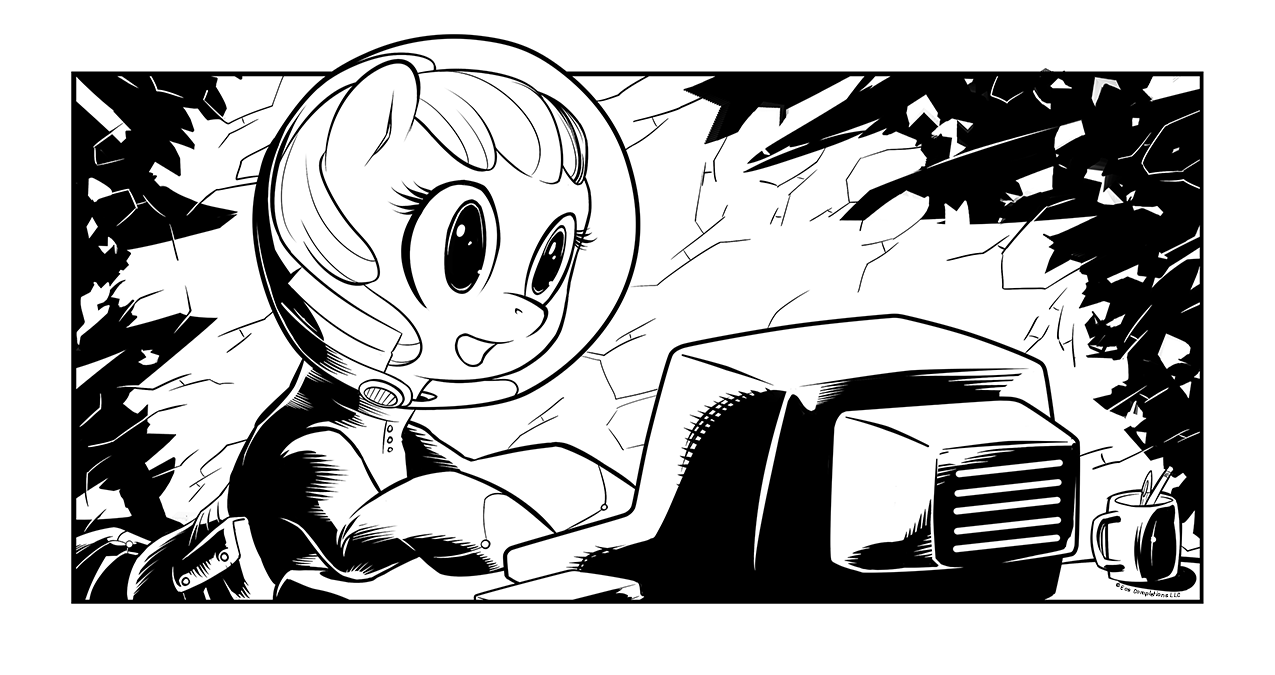
\includegraphics[width=\linewidth]{image15.png}

\begin{intro}
    Psychiatric Help 5¢ - The Doctor is IN
\end{intro}

\englishdaytimeplace{12}{10:30 A.M.}{Broccoli Fields, Big 52 S Branch}

Broccoli, the capital of\dots well, you guessed it. All around the town rose fortified farms surrounded by green and yellow fields; the crop didn't seem healthy nor yummy, but growing anything in this tainted and sunless land already seemed a great success. A couple of figures in the distance were working in the fields, but they didn't pay any attention to the yellow filly moving from the north along the Big 52; unlike the farmers, a solitary spritebot patrolling the road immediately noticed the yellow bolt and stopped broadcasting its usual patriotic songs, instead turning towards the incoming filly.

``Hi Puppysmiles, have you got a mom-'' The filly zoomed past Watcher. ``-ent? Aw, foals! Hey, wait you little lady! Waaait!'' The spritebot chased Puppy trying to catch her attention.

``Sorry Questioner, I'm really in a hurry! I want to get to Broccoli before my mom goes away again!'' The filly kept zooming while she replied to the robot's summons.

``Please! At least tell me what happened in Ivory Tower! I can't follow you into town!''

``Ah, nothing special! Some stars fell from the sky and all the town went boom! It was fun and a little scary, but mom wasn't there so it's alright!''

``Yes, but what made those 'stars' fall?'' insisted the robot.

``Ah, I don't know\dots'' The filly stopped abruptly, suddenly realizing something. ``Oh no! I forgot it! Stoopid Puppy! Stoopid, stoopid!'' The foal began hitting herself on the helmet with a hoof.

``What now? What did you forget?'' From the robot's voice it was easy to tell he was both worried and stumped. ``Was it important?''

Puppy jumped down from the scooter and trotted towards a rock, hitting it with her head and continuing her mantra. ``Stoopid!'' BONK! ``Stoopid!'' BONK! ``Stoopid!'' BONK!

``Stop that! You'll break your helmet, Puppy! Now please calm down and tell me what's wrong, maybe I could help you or find somepony that can help\dots'' The spritebot floated next to the filly in yellow, bumping gently against her shoulder. ``C'mon, you're a big pony, I'm sure it's nothing that can't be solved\dots''

``No!'' BONK! ``You don't understand!'' BONK! ``It's too late nao!'' BONK! ``Stoopid!'' BONK! ``Stoopid!'' BONK!

``Oh, c'mon Puppy, you remind me of\dots'' The robot's voice stopped for a moment, as if he caught himself thinking about things he didn't want to recall. ``Ah\dots I'm sure we can fix it; I'm your friend, don't cry little one and tell me what's wrong, we will find a solution, okay? Just\dots don't do like that\dots please\dots'' The robot's voice was filled with pain and sadness.

Puppy must have caught the change in Watcher's voice, because she stopped headbutting the rock, sat down and sighed. ``I\dots I forgot a very important thing, Mister Questioner, but I had to do it when I was in Ivory Tower and now that the stars are fallen and the place is gone I can't do it anymore\dots I am a silly pony\dots''

``Oh, I understand\dots you needed to be there\dots I'm sorry, Puppy\dots really\dots'' The robot floated beside the little pony for a while before asking, ``By the way, what was that you had to do?''

``I\dots I had to ask a falling star to find my mom\dots there were so much of them, they would find mom for sure\dots when you see a falling star and you make a wish it will come true for sure! But I forgot! Now I have to find mom myself again!\dots it's not fair\dots''

``You forgot to wish upon a star!? All this scene about a wish? I can't believe I-'' The robot paused, noticing the crushed spirit of the filly and rapidly changed tack. ``It's bad, but it's not that terrible, don't worry\dots'' There was a long embarrassed pause, ``Puppy, I had a friend that sometimes acted exactly as you are doing right now\dots she was a very smart pony, but she lost herself in a glass of water because of the most incredible details\dots sometimes it was really important, some other times it wasn't, but her way of panicking and acting impulsively worsened things a lot\dots panicking is not good for clever young fillies; you are a clever young filly, right?''

Puppy sighed and nodded, looking down.

``Perfect, this was what I wanted to hear; since you are a smart pony, I'm sure that you don't even need the help from a star to find your mom. I mean, look at you: you already arrived here without those useless stars, you can go wherever you want with your determination and your friends.''

The filly tilted her head a little, looking at the spritebot with a hopeful expression. ``Really?''

``Yes Puppy, really. I think that if there is a pony that could really find your mother is not a magic pony living on a star or some sort of fairy pony with butterfly wings. That pony is you, Puppy. So, why you don't stop moping and show me some of your enthusiasm?''

Slowly, the frown on Puppy's muzzle turned to a faint smile and kept growing, until Watcher's words hit her little head and she understood them. ``Yush! I'm Space Captain Andromeda! I am the best pony ever! I will find mom for sure! Who need a stoopid star anyway? Thank you Mister Questioner!'' The filly hugged the spritebot, giggling. ``I'm sure mom will be in Broccoli or in the town after Broccoli at worse! I'm almost there! YAY!''

The voice chuckled. ``This is the spirit, Puppy! Now go and get 'em! Oh, and it's Watcher, my name is Watcher\dots''

``Sure Mister Questioner!''

``Not Questioner, Watcher!'' insisted the spritebot.

Puppy sighed, trying to be patient. ``Really, i don't see you watching a lot, but for sure you make a lot of questions, so if you really want a name like that, it's Questioner, no more complains.''

``But it's not my name!'' protested the voice.

Puppy shrugged. ``Now it is, live with it. Really, no other voice protested when I gave them names.''

``Aw, I give up\dots do as you want, stubborn little pony\dots I have to go, just try to stay out of troubles, okay?''

``I stay always out of troubles! I'm a good filly!''

Watcher chuckled one last time, before the voice was replaced by the usual patriotic music and the spritebot floated away.

Puppy watched at the robot disappearing behind a hilltop and sighed. ``I can't see why he doesn't like the name I gave him\dots I mean, it's so much better than the one he had before!''

\horizonline

\englishdaytimeplace{12}{11:30 A.M.}{Broccoli, Big 52 S Branch}

The town of Broccoli was protected by a group of local guards and a couple of squads from the Hired Hooves; not a real army, since nopony was supposed to threaten the town. From the night before, the guards were now running double shifts keeping all their eyes pointed toward south; from what little news Lonesome Pony gave, the Wild Herd was on the war path and this time they had sticks, so it was vital that every pony who could use a weapon was always ready to get up, grab his rifle and defend the wall.

The mercenaries wore black gas masks and heavy armor, nothing special if compared to a steel ranger's power armor, but for the Wasteland they were still equipped top notch. All of the Hired hooves sported anti materiel rifles or assault rifles, while the Broccoli militia was a little more lightly armed and way less armored.

A pair of militia ponies patrolling the northern fields noticed Puppy approaching along the road. One had already taken aim when the foal suddenly came to a halt and sat down, holding one hoof against the side of her helmet as if she were listening to something. The pair looked at one another in confusion.

``Attention. Incoming request of opening a communication bridge with structure Solaris Stable. Checking authorization. ID is valid. Opening communication.''

SolOS' voice replaced that of the suit's. ``All these ID checks are annoying, they could prove to be a problem in case on an emergency, I suggest you to lower your security measures.''

Puppy sat down in the middle of the road, smiling. ``Oh, it's you Blue Voice, how are you?'' The filly waved a hoof at the approaching guards, who simply waved back and exchanged another confused glare.

``The plan is not going as predicted, D018, this is why I am calling you. I have some questions for you.'' SolOS hadn't even bothered to say hello, but Puppy knew he was just a bit shy, so the filly let that thing slip.

``Questions? Guessing game! Yay! Ask me, I'm world champion of guessing game!'' The filly clapped her hooves in joy, she loved to play.

One of the two guards levitated his rifle, readying the shot, but the other stopped him with a hoof. ``Wait, I think this is that ghost from the radio; I don't think we are supposed to shoot her\dots besides, I'm curious.''

SolOS went on, ``I have contacted the facilities at Solaris Tunnels 1 and 2, but in tunnel 2 I found some sort of Artificial Intelligence controlling the place. Since you once said something about being friend with other A.I. I wanted to know if you knew something about this one. Its designation code is P7.''

``Oh, Miss Voice! She is my very best voice friend! She is funny and friendly and she is the best funnybot ever!''

SolOS paused for a moment. ``I take that as a yes. That program was not supposed to be installed in a military base, do you know why there is a P7 pony machine interface operating in Solaris Tunnel 2?''

``Sure! She was lonely at Salt Cube City, so I helped her move house, now she has a lotta new friends! Ah, do you want to be her friend too?''

The unicorn guard sighed, but his friend poked him with a hoof. ``See? She's been in Salt Cube and at the Tunnel, she must be the Ghost. Wasn't she looking for her mother or something like that?''

The unicorn shrugged. ``I don't care, look, if she is the pony you are talking about we should simply ignore her and keep our eyes open for some real threat.'' The two ponies trotted away, taking a path that headed to the nearest farm.

In the meantime SolOS and Puppy continued to talk over the radio. ``Actually, I want it to grant me access to the weapon storage, but that program cut me out from any administration rights and banned me from the local net.''

``So, ah\dots You wanted to be her friend but she didn't want?''

``No, I need to get access to the weapon storage. Are you even listening to what I say?''

Puppy giggled. ``Silly Voice, you don't need to be shy! She is a super friendly Voice and I am sure that she wants to be your friend and you two will be best friend forever, because you are blue and she is pink and everypony knows that pink is the color of fillies and blue the color of colts and-'' Puppy stopped, gasping.

``What now?'' SolOS voice had grown annoyed; as usual talking with that crazy anomaly was an impossible feat.

``I know! You have fallen in love with her! Don't worry! I'm fixing that! I'm a super expert of love!''

``What? No! That's not what I meant at all! Talking with you is a complete waste of time! I'll find another way to get those weapons, get lost!'' SolOS cut off the communication.

``D'aww! He's so shy!'' Puppy finally turned toward the two guards. ``Hi, I'm Puppysmiles! Have you seen my mo- hey where have they gone?'' The guards had disappeared, leaving the foal on her own.

\horizonline

\englishdaytimeplace{12}{12:00}{Broccoli, Big 52 S Branch}

Puppy reached the walls of Broccoli still confused about being left alone like that; this had never happen to her before; well, except that one time in Sun City, but it was different; ponies there were weird. Oh well, it didn't matter, there were plenty of pretty ponies here, so it was going to be easy to find some help.

The foal found herself in front of a closed gate and sat down, looking up at the wall's crest; a pony with a gas mask was looking back at her. ``Hi there! Can I get inside Puppy please? I'm looking for my mom! Ah\dots if I can't get in, can you tell her to come out?''

The masked pony ignored the filly and trotted away, patrolling the wall. ``Hey, I'm talking with you, funny muzzle! Aw! HEY!'' Nothing, these stoopid ponies had to be deaf and blind\dots what now? Puppy tried banging at the door, but patience wasn't exactly her virtue, so she decided to trot around the wall and see if there was another way in.

The wall was composed of a patchwork of metal carcasses, welded together to ensure that there were no gaps between them. Suddenly Puppy heard the sound of gunshots coming from the south, quickly followed by the shouting of guards as they rushed around the walls towards the noise. None of them paid any attention to the foal outside.

When the filly reached the other side of the town, she noticed that there were way more ponies on the walls; a lot of them were wearing those black masks and some others had helmets and crappy rifles. Sometimes a pony looked down at her, but when she tried to talk with them they simply turned away and resumed looking out into the distance just like their friends were doing. This was beginning to frustrate the foal. ``Ah, Mister Voice, isn't there any secret passage to get inside?''

``{\mt Analyzing. Connecting to Equestria Cartography Onspark. Warning. Broccoli not found in the database. Switching to auto map mode. The town has two access points, one from north and one from south. Both accesses in this moment are inaccessible.}''

Puppy sighed. ``So, we are closed outside?''

``{\mt Affirmative. A rapid analysis of the external walls doesn't reveal the presence of any other entrance. Advised solution: asking to be let in and waiting for a positive answer.}''

Puppy frowned. ``Wut?''

``Knock at the door and wait.''

The foal smiled enthusiastically, finally understanding what the interface meant. ``Oh, okie dokie! I can do that, I'm good at asking things!'' The filly trotted merrily toward the southern door, only to be interrupted again by the suit.

``{\mt Attention. Incoming request of opening a communication bridge with structure Solaris Tunnel 2. Checking autho-}''

The suit's voice was muted and replaced by P7's. ``Aw, shut up you grumpy routine! Hi Puppy, how are you? I hope you're fine because it has been a while since our last chat and I was really worried that you forgot about me, so I was thinking that I should call you just to be sure you were alright\dots ah\dots are you alright?''

Puppy jumped on her hooves in excitement. ``Miss Voice! I almost forgot to call you! I have a lot of things to tell you! Oh, oh! But wait! I have super duper extra news for you!''

``Really? Wow! I can't wait to hear it, but before I wanted to ask you why you activated the Ponymedes net. I mean, you said you didn't want ponies to get hurt and then-''

"You have a coltfriend!''

``And then you have a coltf- wait, I have a what? Why am I the last one that finds out these things!?''

Puppy nodded wisely. ``Yup, but he's super shy and he say you were a little nasty with him\dots''

There was a short pause, while the A.I. Tried to elaborate the new information. ``But I don't have a coltfriend! I don't even know anything about love!''

The foal frowned. ``You don't know anything about love? How's that possible?''

``Well, you see, it seemed that love trashed the P5 project, since the AI decided that love was more important than, let's see\dots survival of the planet, so she mixed up her priorities a bit and\dots well that's a sad story, you don't really want me to tell it. But now that I have a coltfriend it's all different! What can I do? I don't even know him!''

Puppy giggled. ``Silly voice, but he knows you! And don't worry, I am the best love expert ever!''

``Really!? Woah! I always always ALWAYS wanted to know about love! Can you teach me?''

The filly held up a hoof. ``Yush! Doctor Puplove will teach you and you will be best lover ever!''

``YAY!'' Now that the long dead foal and the party A.I. had a real topic to discuss, trivial things as the utter destruction of a pony settlement and unleashing a weapon of mass destruction rightfully slipped away from their attention.

``First lesson, the dangers of love: cooties!''

\horizonline

\englishdaytimeplace{12}{12:30 P.M.}{Broccoli, Big 52 S Branch}

Two of the guards on the wall were looking down at the foal as she talked and giggled to herself, while their fellow sentries kept watch for any sign of another suspicious movement from south. One of then scratched his head and muttered, ``We should at least tell her to go away\dots''

The second guard sighed, hitting his friend on the head. ``Yeah, sure, are you going to tell her that? After we've seen what happened to the rangers at Ivory Tower? No thanks! You heard the radio, she is dangerous! Let's wait until she gives up and moves away.''

``But, if she doesn't go away? Then what? I think that somepony should go down there and shoo her.''

``Sure, great idea, and who's going to tell her that? You?'' The elder guard emphasized the concept by knocking his colleague on the head again.

``Hey, stop hitting me! Why don't we send the mayor? We elected her for this kind of thing, after all!''

The veteran stopped his hoof a moment before hitting the other guard for a third time, and instead he tapped his chin. ``You know? that's not a bad idea\dots not bad at all\dots''

\horizonline

\englishdaytimeplace{12}{12:45 P.M.}{Broccoli, Big 52 S Branch}

Half an hour of explanations later, P7 knew everything she needed to know about love, at least from Puppy's point of view.

``Alright, so, kisses are eeew but they are cool if they have explosions in the background or a fitting music?''

``Yep.'' Puppy nodded with the expression of a pony who knows a lot of things.

``Still, I'm not sure I understood the part with making foals\dots''

``Eh, that's quite a difficult part; I'm almost sure that there are a mom and a dad involved\dots mom told me that you had to love dad very super much and it involved a letter to Pretty Princess Celestia, but the teacher at the kindergarten told me a story with cabbages and Pretty Princess Luna\dots my old school friend Green Sleeves told me it involved also a lot of rumbling and that it was super gross and that when she had caught her mom and dad on the couch they got super angry and her mom scolded her dad because he didn't lock the door and the day after she explained to Green Sleeves that they were giving her a little sister\dots'' Puppy paused for a moment, trying to remember something else. ``I think that sending a letter is better; it also explains why I can't have a foal of mine, since I can't write\dots''

``Alright, and what about poetry?''

``Oh, that's easy; to fall in love you look out of the window and then your real love will come out of a bush and sing you a song, or tell you some mighty beautiful poem and you will love him and all.''

``That doesn't sense very much\dots'' objected the computer.

``Love doesn't make sense at all. Besides, I've seen it in a show called Colteo and Fillyet; it was boring as hay and boring things are always instructive, so it must be true.''

``Okie dokie! You are the expert here!'' replied P7, now positively convinced. ``So, what do I do now? Who is this lover of mine? I'm so excited, aren't you excited? When am I going to meet him?''

``Woah, hold your horses! He must do the first move! It's always the colt that goes to the filly, not the opposite!'' Puppy sighed. ``Really, were you listening before? I'll call him and tell that you don't like him at all, then-''

``Hey you there\dots'' A voice called, but Puppy was far too busy with matters of the heart to pay attention.

``But I like him! I want to meet him, but you didn't tell me his name!'' protested the A.I.

Puppy helmethoofed. ``Of course I didn't tell you! He's a secret admirer! Do you want to spoil everything? Do you want to lose your true love forever?''

``Ah-hem\dots Excuse me!'' The voice interrupted again but the foal waved a hoof at it, trying to get it to be quiet.

P7's voice panicked. ``No, NO! I don't want to be alone for all of my existence! I'll do like you say Puppy I'm completely in your hooves! Please don't let me down!''

The filly nodded, satisfied. ``Very well, stick to my master plan and you will be happy ever after.''

``Hey, stop ignoring me, little filly!'' A hoof knocked on Puppy's helmet forcing the foal into diverting her attention from Miss Voice's love affairs to the annoying pony in front of her.

She was an earth pony mare with a helmet, a light combat saddle and a lever action rifle standing directly in front of Puppy, with an annoyed expression. ``I'm the sheriff and the mayor of Broccoli, you can't stay here; please go away.''

Puppy sighed. ``Excuse me, Miss Voice, it seems that some ponies can't really wait their turn\dots I'll call you later.'' The filly moved her attention toward the mare and her annoyed expression quickly changed to a broad friendly smile when she realized that the pony came from inside the wall. ``Hi! I'm Puppysmiles! Have you seen my mom? I tried knocking at the door but nopony opened it for me and all those funny faces up on the wall must be completely deaf!''

The mare sighed, waving a hoof. ``Wait, stop talking and listen! You can't come inside the town. There are raiders all around the place and you are not welcome here. I'm here to tell you to go away, we don't want you.''

Puppy kept smiling while she replied. ``Silly pony, I can't go away! Mister Voice says that my mom is inside this place! I have to find her so that everything will be alright!'' The little pony giggled.

``What the\dots are you stupid or what? You arrived from Ivory Tower and that place was completely destroyed just the other day, we aren't a superstitious herd, but it seems quite obvious that you don't bring good luck with you, so just live with it. You can't get in, now go away or we will shoot you down.''

``But I need to find my mother! Puppy please?'' Puppy tried her best begging eyes, making the pony step back for a moment.

``A no is a no! Now go away or you will be killed. This is my last warning.''

The little filly sat on ground, looking at the mare while pouting. ``B-b-but\dots my mom\dots please\dots please!'' The foal began sobbing.

``No\dots please, don't cry! Aren't you supposed to be some sort of immortal hero?'' The mare had been prepared to send away a big badass wasteland dweller, but a crying foal was not on her list. This little pony had no dignity at all; the mare looked up to the walls, begging for some help from the mercenaries, but all she got back were just shrugs. \emph{Damn, this filly saved their families, they won't shoot for sure\dots} ``Okay, okay! You win! Just\dots don't cry, alright? Stop crying! You can come inside and I'll accompany you through the town, so that you can look for your mother!''

The foal sniffed a little, muttering her reply. ``You don't want to find my mom for real\dots you just want me to go away\dots why you don't want to be my friend, miss pretty pony?''

The mare snorted. ``Don't make me change my mind! We will get inside but you have to follow some rules! No weapons, no stealing, no annoying the guards and the most important one: stop whining!''

Puppy smiled and trotted to the mare. ``Okie dokie! I like you miss pretty pony! What's your name?''

The guard sighed and looked away. ``Boiled Broccoli. Now behave and follow me.''

``Eww! I don't like broccoli! How can a pony have a broccoli cutie mark? It's terrible!'' protested Puppy.

``Broccoli is all we have here, you better learn to like Broccoli because you won't get anything else for lunch, dinner, breakfast or a snack. Oh, and they aren't for free.''

\horizonline

\englishdaytimeplace{12}{13:30 P.M.}{Broccoli, Big 52 S Branch}

The mayor of Broccoli stepped inside the town hall while talking with Puppy. ``Alright kid, here we are: Rainy Days Hall. I'm not sure that it has something to do with your mother, but the town hall was here since the days of the war; it's name comes from all the writings on the walls. Take your time.'' The mare took a look back at Puppy to see if the foal was listening, but her charge was instead engaged in conversation with her own helmet. Boiled Broccoli shook her head.

``So I told her that you were super shy and she seemed really interested; now you must write her a love poem.''

``You called me just because you want me to declare my love to another artificial intelligence? I have a lot of things to do, like keeping together a band of brainless cutthroats and you call me for such an idiocy? Please, tell me, did I do something wrong?''

Puppy stopped for a moment, pondering SolOS' question before nodding. ``Yup totally, but we can fix that and she doesn't really know that you were a bug and a stinker. Now, about that love poem\dots''

``I don't want to write love poems! Stop calling me!''

``D'aw! You're so sweet! Okie dokie, I'll help you with this one! Tell me, what do you like in Miss Voice?''

``Ah, she has a surprisingly powerful firewall and her routines seem to work better while she is multitasking\dots I also found that her anti-virus suite was well programmed and up-to-date and- wait, why am I playing your game? I'm out of here and STOP. CALLING. ME!'' With these last words SolOS closed the communication, leaving Puppy alone with Broccoli's Town Hall.

The mayor sighed, looking at the foal. ``So are you done? Want a cup of tea?'' The sarcasm was evident in her voice, but using sarcasm against puppy was just like honking a horn to make a deaf pony move.

``Ah, no thanks, I can't take off the helmet\dots'' The filly stepped in the large room filled with lots of chairs and a large desk; on the entrance's left there was a line of windows looking outside, but all the other walls were covered with graffiti. Puppy couldn't remember being in this place before, so she hadn't the slightest idea of where to look.

``Ah, can I has some help, please?''

Boiled Broccoli sighed. ``What now? Can't you even read?'' The mare pointed at the walls. ``It's all there!''

The foal looked away, a little embarrassed. ``Ah, it's not that I can't read, but\dots well\dots I have problems with some letters and I'm not very good with long words\dots''

``Listen, I've read all this stuff like a hundred times, it says that one day a mare named Rainy Days arrived here from a military base in the north and founded the place; there were troubles and ponies were dying, so she wrote some important rules on these walls.'' The pony pointed at a long list of written words placed just behind the big desk. ``See? They're still there\dots anyhow, she had been the first mayor of this place as you can see on the mayor's list there, but after her there were at least five other Rainy Days\dots it's a pretty common name around these parts\dots''

Puppysmiles tilted her head, trying to understand what the mare was telling her, but everything she got from her fast synopsis could be summarized like this: ``Wut?''

Boiled sighed. ``Why me? Listen, we are in a situation of danger here; a big band of raiders is assaulting the city south of here and they could be hitting us very soon. I have no time to help you finding a two hundred years old mare! Please, go away and leave us be! There is nothing for you in this place! Honest!''

Puppy frowned; she didn't understand everything, but it seemed that her mom had been here and now was gone\dots again\dots if only this pretty pony could tell her where mom went this time it would have been awesome, but it seemed that she didn't want to help Puppy.

``Ah, if you help me, I'll give you this\dots'' Puppy looked inside her bags, searching for something pretty to barter. ``It's a barter, it's okay because everypony does that!'' The filly found Fuzzy Ball, but she didn't want to give away her pet\dots no, it was better to keep Fuzzy hidden before somepony noticed her\dots there were many other things that she could offer, like some empty bottles of Sparkle-Cola, a bag of pretty caps, a brushabe Lyra\dots wait, what?

The foal gave a better look at the doll to be really sure, but it was impossible not to recognize that gorgeous coat and wonderful flowing mane. ``Woah! He gave me the pretty green pony! Look!'' Puppy showed the green plastic unicorn to Boiled Broccoli.

``What now?'' The mare raised an eyebrow, confused.

``Mister Red Cape! He gave me his doll! She is so cute! I love her!'' The filly hugged the doll in a burst of happiness. ``This is the best toy ever! She still has all her mane in its place! and her tail too!''

The outburst of joy made the guard pony smile for a moment, but she immediately reverted to her scowl; foals were annoying, that was all. ``Yes, so what? Are you trying to make me help you in exchange for a doll?''

Puppy froze on the spot, her joy disappearing in sudden realization. ``You\dots you want her? B-but\dots'' The foal looked at the mare, then a the doll and again at the mare, hesitating. This toy was really beautiful and it was so new, but Miss Broccoli wanted it in order to help Puppy finding mom\dots

Sacrifices, always sacrifices\dots why this stoopid place was taking from her every single nice thing she had? Not fair, not fair at all; but these were the rules and mom was somewhere out there. ``Ah\dots if you help me finding mom\dots'' Puppy hesitated before nodding, resigned. ``Okay, I'm giving you the cute doll. But please, will you help me?'' This was a hard blow, the doll was a present, but mom\dots no Puppy, don't think about it; when you'll find mom all of this will go away. Just one more town.

Boiled Broccoli cocked her head. \emph{What the fuck, is she holding back tears? Does she really believe that I want her doll? What am I doing, teasing foals and extorting toys? When did I become like this?} The mare looked away, lowering her voice. ``I\dots I might help you. I think that there is some sort of computer with a logbook; we can search together in the first entries to see if there's something regarding this Rainy Days\dots come with me.'' The little pony inside the guard felt very, very ashamed of herself.

\horizonline

\englishdaytimeplace{12}{14:15 P.M.}{Broccoli, Big 52 S Branch}

``Could you please speak a little lower? I'm trying to find some clues about your mother while you play Cirano de Puppysmiles!'' Boiled Broccoli groaned, trying to ignore Puppy's chatting on the radio and put her hooves over her ears.

``Yush! He says he's super in love, he likes your\dots ah\dots stuff, and some other stuff of yours and he said something about a wall that burned; I didn't understand everything but he seemed so hot!''

P7's voice was dancing the pony pokey out of joy. ``Yay! He likes me! I'm so happy I can't believe I don't even know who we're talking about! You know, after that hacking attempt from the other day I was quite depressed; it seemed that anything out there existed with the sole purpose of bullying me, but now that I have a secret lover my life is pink!''

``Yep, I know I'm the best, no need to thank me\dots now, your next move is waiting until he confesses himself, then you refuse him.''

There was a long pause. ``What? I think I heard you wrong. This is funny, it seemed to me that you told I had to refuse him.''

Puppy nodded wisely. ``Pressis- precis\dots pree- ah\dots eyup! You must always refuse him the first time, so he feels bad and loves you even more! Remember the rules!''

``Oh, right, the rules! Okie dokie, let's do this by the book! I'll leave everything to your master plan then!''

Puppy smiled. ``Don't worry, you won't regret this! Now I really have to go because miss Broccoli is trying to find my mom, I'll call you later and tell you what to do, okie dokie?''

``Okie dokie Loki! Later!''

The communication was interrupted while Puppy turned her attention toward the pony at the terminal. ``Ah, did you find something miss pretty pony?''

``You mean, while you were giving sage advice about love to your friends? Yes, I found something.'' The mare turned the computer screen towards Puppysmiles. ``Is this your mother?''

The filly smiled happily. ``Yes! Mom! Isn't she beautiful! My mom is the best mom ever!'' It was a repertory photo, with the mare wearing her military technician suit and a helmet; the earth pony was slim and not very tall, Puppy shared the line of her muzzle and her eyes.

``Alright, here it says that she moved south, to Emerald Shores\dots doesn't say why, but it was almost two centuries ago\dots I don't think that-''

``Where is Emerald Shores?'' Puppy Asked promptly.

``South, past Ironworks; you can't miss it because there's only ocean past Emerald Shores.''

Puppy's ears moved a little. ``You said\dots That place is the last one along this stoopid road?''

``Yes, it's the last city along the Big 52, but you shouldn't call it-''

``YAY! I found mom! There's no other place where to go! Mom is in Emerald Shores!'' The filly jumped all around the room, faster than a filly on a sugar bomb and Sparkle-Cola trip.

``Well, actually if you follow the coast there's the NCA and\dots you don't give a fuck, right? You aren't even listening anymore.'' The filly was already out in the road and was running toward the walls; Boiled Broccoli sighed. ``Oh well, at least I got rid of her\dots''

Trotting outside the town hall the mare was surprised to find Puppy waiting for her, especially after having seen her zooming away. ``What now? Weren't you chasing your mom?''

The foal took the green unicorn doll from her bag and offered it to Boiled. ``Ah, please love her and brush her. Her name is Lyra and she is a really really awesome friend\dots''

The guard refused the doll, sighing. ``Keep that thing; I'm not stealing toys from the foals\dots just get out of my town as soon as possible and don't come back. We already have our load of troubles.''

Puppy hesitated a moment.

``But, if you want, I can take the doll anyway\dots''

That last line gave the filly the motivation she needed to move; the foal hid the brushable toy in her bag and zoomed away, leaving alone a snickering Boiled Broccoli. ``'kaythankyoubai!''

``Goodbye, whiny ghost\dots'' The mare sighed one last time, then raised her voice yelling at the ponies on the walls. ``Let the foal go out and close the doors again! Organize for another night with double shifts! Make sure every farm lights a fire and keep your eyes open!''

Winds of war were blowing in the air, and that yellow pony was running straight into the storm\dots oh well, not Boiled's problem at all.

\horizonline

\englishdaytimeplace{12}{17:00 P.M.}{Broccoli Fields, Big 52 S Branch}

``What do you want again?'' SolOS' exasperation was palpable in his voice, but Puppy didn't care.

``Hi Mister Blue! I've talked with Pink and she is very, very interested in meeting you\dots she said she feels so lonely and wants new friends.''

``What the\dots wait, you convinced that Artificial Intelligence in Solaris Tunnel 2 to let me access its storage? Are you serious?''

While zooming through the last fields south of Broccoli, Puppy frowned. ``I am always serious! Yes, she is waiting for you to sing her a serenade, so, make a super romantic song and go to her, so you will fall in love and you will be happy ever after!''

There was a long pause before SolOS spoke again, and when he did so, he was confused. ``Ah\dots thank you? I was convinced this P7 was a friend of yours, can I ask you why you are backstabbing her like this? It doesn't seem rational\dots not that I expect anything rational from you anyway.''

``Backwhat? Listen, it's easy: you are a Voice, she is a Voice and both of you are very, very lonely. I'm mighty sure that when you will meet you will be super friends and since I am friend with both of you I want you to be friend with each other! That's all!''

Another long pause rolled away with the road before SolOS replied. ``Friends, you say? We'll see\dots I could use a strategic ally, after all\dots'' When the communication was cut, the radio replaced Mister Blue's voice.


{\rt Tonight I can't say it's a good night, my little ponies. Not earlier than half an hour ago, Ironworks launched a cry for help. The ponies in the fortified town are under siege, apparently attacked by an horde of well armed and organized raiders. If this is the Wild Herd, we have never seen them like this before; they have heavy weapons, combat robots and fight like an organized group. I have no idea of what's going on behind the scenes, Big 52, but if we don't react now, it could be too late, and to show that Lonesome Pony is not all talk and no meat, I'm flying to the front with my old rifle on my shoulders. DJ Good Stuff will take care of the radio in my absence, be kind with her and help her like you did with me. From L.P. That is all, have a last song.}

\begin{song}
    Blessed bodies of the Heavens

    sun and Moon of greatest light

    bathe us in your warm embraces

    shield us with your peerless light

    help us to stand firm as mountains

    doing right and shunning wrong

    may we find our strength in friendship

    unite our herd as one group strong
\end{song}

~\vfill

\begin{engnote}
    Level up! (14)
    
    New perk added: Boisterous Incompetence - Yeah, don't worry I know exactly what I'am d-BOOM! During dialogues or skill tests, if your skill is less than half the required score for succeeding in the feat, you get special dialogue options that have a 50\% chance of success. Beware, if you fail this test, the results will be way worse than a usual failure.
\end{engnote}



\chapter{Reunions}

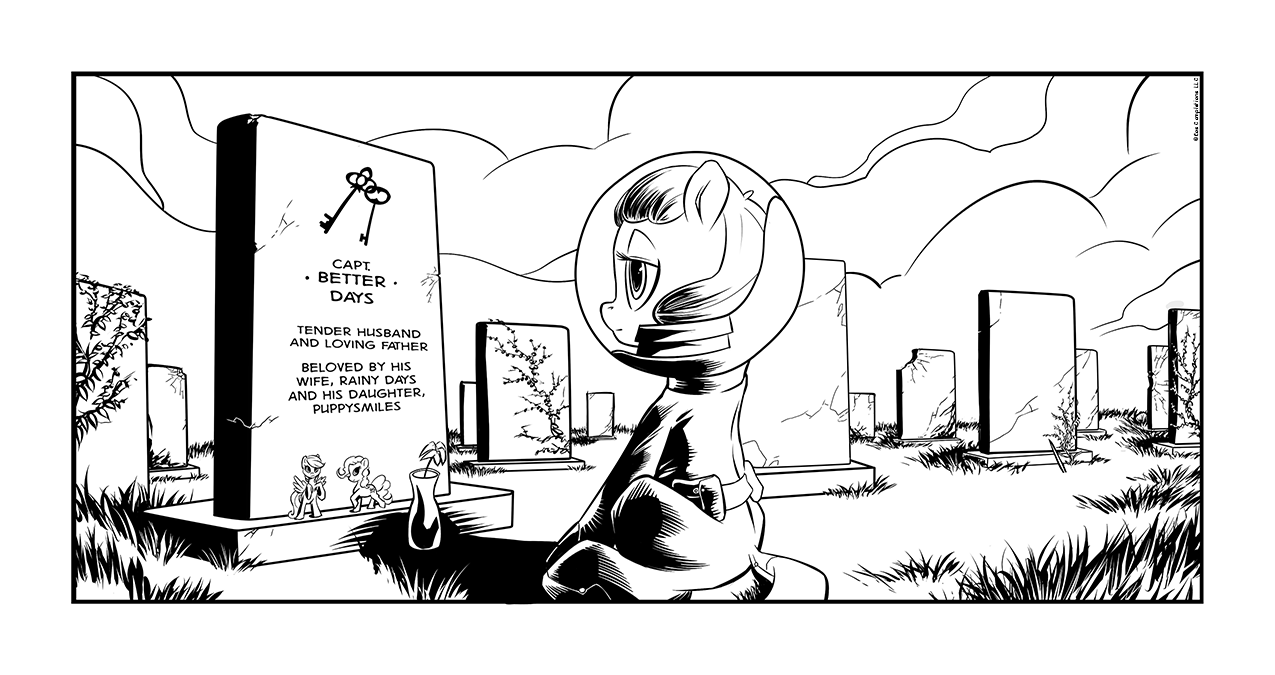
\includegraphics[width=\linewidth]{image16.png}

\begin{intro}
    We're getting the band back together
\end{intro}

{\rt 'Sup, ponies. I can't believe he really did that! He took that piece of crap he calls a rifle and just flew away\dots that feather head! While I was sleeping! Hey L.P. if you are listening to this, shove that rifle up your ass!}

The radio paused for a moment, the feminine voice that had been talking didn't seem sad or worried, just angry.

{\rt Alright ponies, show must go on; DJ Good Stuff here and you are listening to Radio 52, at least until I collapse because a certain pony left me here all alone with a show that is never supposed to stop! Okay, new rules: I'll be airing during daytime and you'll get only music during night, because I'm not immortal and i need to sleep, and if anypony wants to drop by and do some talking while I'm asleep, just knock at the door; you know where we are.}

The sound of paper shuffling filled another pause.

{\rt Alright, remember that I can operate that damn shortwave radio too, so don't stop sending news, especially regarding the situation in Ironworks. And speaking of news, the Memorial has been deserted and the ponies are moving north, towards Broccoli. All the caravans still moving between Broccoli and Emerald Shores should head north and try to reach Rust Manor. I repeat, head north towards Rust Manor, don't stop at Broccoli because it's too near to the war zone.}

{\rt Fuck, I hate giving the news; if anything else comes in I'll lat you know, otherwise you'll get music all day long. Remember, music means no news and no news is actually good news. Have some angry music because I'm angry and give Lonesome a buck in the head if you see him.}


\begin{song}
    Say your prayers, little one

    don't forget my son

    to include every pone

    tuck you in, warm within

    keep you free from sin

    `til the sandmare she comes
\end{song}

\horizonline

\englishdaytimeplace{13}{4:00 A.M.}{The Memorial northern picnic area, Big 52 S Branch}

In the distance ahead of Puppysmiles stood another little town, little more than a group of shacks built around a very large statue that depicted a group of ponies hoisting an Equestrian banner. The marble monument was remarkably well conserved, it's enormous size made it possible to see even from several kilometers away. On her way south the filly met several groups of ponies with carts loaded with everything; she tried to socialize with them, but they simply kept moving, mostly ignoring Puppy except for a couple of foals who waved back from a cart\dots Entire families were fleeing, leaving their homes and trying to reach safety behind the walls of larger and better guarded settlements.

The filly was now staring at the monument with a puzzled expression. ``Ah, Mister Voice, are we near to dad's place?''

``{\mt Analyzing. Actual position is Equestria: Fallen Soldiers Memorial, northern picnic area. Location of your male parent is currently unknown.}''

Puppy tilted her head, studying the surroundings. ``Yes, I remember this place! That big road sign with the Pinkie Pie face and\dots'' The foal left the road, galloping over a low hill and finding herself in the middle of a group of tables and rusty abandoned barbecues. ``This is dad's place! Dad is near! Let's go!''

The filly in yellow galloped further away from the road, heading for a group of hills to the west. The low hills were still far from here, approximately four or five kilometers away from the Memorial, but even from this distance it was possible to see that they were dotted with white stones, each spaced evenly apart.

As she ran toward the distant hills, Puppy passed by a dead tree; once upon a time it must have been a proud oak, but all that was left now was just a blackened skeleton, its trunk scorched and its branches bare.

\emph{``I want more apple pie!''}

\emph{The grass was green and birds were singing among the leaves; the sky was blue and everything was so nice\dots}

\emph{``Don't eat too much Puppy, we still need to go to dad's place, remember? If you eat too much you'll get sleepy and you don't want to be sleepy when we go visiting dad, right?''}

\emph{``But mom, he's never there! We went a lot of times and he was always away! Will he be there this time?''}

\emph{``I\dots I don't know, Puppy, but you can leave him flowers, so he will find them and know that you love him, okie dokie?''}

\emph{A couple of colts chased each other, disappearing behind a hill; there were ponies playing and ponies having lunch, everypony was having a good time.}

\emph{``I got a better thing this time! Look!''}

\emph{``Oh, but Puppy, that's a toy of yours\dots are you sure you want to leave it here?''}

\emph{``Yush! So when dad will be back he will play with it and won't feel lonely! Besides, he will return it to me when he comes back home again!''}

\emph{``\dots''}

\emph{The distant sound of laughter filled the silence between mother and daughter.}

\emph{``Mom? Why are you crying?''}

The filly stopped for a moment, looking at the big tree and trotting around it\dots she could clearly remember having a picnic in this place not earlier than in spring\dots where had everything gone? Oh well, she knew that trees sometimes lose their leaves because mom had told her so and since there wasn't even grass on the ground it was just fitting. The filly trotted away toward the cemetery.

\horizonline

\englishdaytimeplace{13}{6:00 A.M.}{Interequestrian 52 War Cemetery, Big 52 S Branch}

The tombs were all similar, consisting of small marble stones on which were engraved a name, a date, a cutie mark and a few short words. Some stones were white and other stones were black, but when Puppy asked to her mom why they were different she simply replied that the ponies napping there were more important than the others\dots Puppy didn't like that reply, since dad was a very important pony but he only had a white stone; so she decided to bring him some more flowers, just to show him that she was super sure he was the best dad ever.

``{\mt Warning. Receiving distress radio signal. Distance from the source: two hundred meters. Signal identified: Device 009. Warning. Receiving new distress radio signal. Distance from the source: two hundred and fifty meters. Signal identified: Device 020.}''

Puppy tilted her head, confused. ``Wut? New radio music? I hope it's not like the last time when there was just a stoopid pony saying endlessly `help me, we're doomed' and all those silliness\dots''

``{\mt Negative. These are Ministry of Peace distress signals from other MK VI Suits. Receiving a third signal on a distance of two hundred and thirty meters. Signal identified: Device 013.}''

The filly sighed. ``Look, if it's not music I don't care. Now let's go find dad, maybe he's back and we will go find mom together.'' With these words the foal headed toward a low hill with the statue of an alicorn on top.

The hill was surrounded by a low metallic fence with several marble arches that led inside that area of the cemetery. A large main battle tank stood In front of the arch Puppy was going through; a brass plaque in front of the war machine explained that in this part of the graveyard were buried the fallen soldiers from the Third Armored Company -- Steel Flanks; there were also some commemorative words and a brief statement that explained how tanks nowadays weren't widely used on the front because of the new technological breakthroughs and that this decommissioned machine had been left here to safeguard its sleeping brothers.

The filly in yellow had been here more than once, so she already knew where to go and headed toward a specific grave; seeing that the place was deserted, Puppy sighed and sat in front of the white stone.

The cutie mark of a couple of keys was engraved on the marble surface, together with some writing:

\begin{center}
    Captain Better Days
    
    Tender husband and caring father.
    
    Beloved by his wife Rainy and his daughter Puppysmiles.
\end{center}

The date was mostly unreadable, but it didn't matter very much to Puppy, since she was mostly interested in the grave itself. On the small mound sat an empty vase and a couple of plastic figures. The vase once contained flowers, but now it was just filled with murky water and covered in mold, but the plastic figures still stood on the grave, looking back at Puppy; they were two molded plastic ponies, like those that were put into cereal boxes. The first figure was a miniature Pinkie Pie, while the other was of Rainbow Dash.

Puppy sighed. ``He didn't take them\dots why he never takes what I leave here? I was sure that he loved Pinkie Pie and Rainbow Dash!'' Touching the plastic blue pegasus with a hoof, the filly continued. ``Stoopid dad, if he was a little more at home mommy could be happy\dots''

Oh well, mom explained plenty of times that it was okay if he didn't come home and that she wasn't mad at him; the filly wasn't completely convinced, but something in her mother's eyes told her that she had just to accept that explanation. From the day mom got angry because Puppy didn't want to come home until dad came back with them too, the foal decided that she didn't want to see her mother cry and scream like that, so she decided to play along and leave something in this place every time she came here, hoping that one day dad would realize that she and mom still loved him and maybe he would finally come back.

Puppy cleared her voice and stated, ``Everything.''

``{\mt Warning. The inventory management spell is not devised to operate more than one object at a time. Opening fast inventory scrolling by alphabetical order. State `next' when you have finished examining an object and need to move on. State `stop' or `exit' when you want to close this application and restore usual inventory management program.}''

An Ashtray floated in front of puppy. ``Next!'' Another ashtray appeared. ``Next!'' Yup, ashtray. ``Next!'' Again, an ashtray ``Next!''\dots did I say that puppy usually scooped up every single shiny object she found on her way? This was going to take a while.

\horizonline

\englishdaytimeplace{13}{7:00 A.M.}{Interequestrian 52 War Cemetery, Big 52 S Branch}

``Next!'' The twentieth fork was stowed back into Puppy's bags and the sorry, dripping remains of Fuzzy Ball floated in front of the foal. ``Ne- no wait! Fuzzy!'' Grabbing the dead parador cub, a disgusting green goo oozed from the cracks in its carapace. The dead creature had lost all of its legs and only had a single wing left, while the eyes at some point started to decompose and were now just another grossly rotting detail on that thing.

``You don't seem very healthy today, Fuz\dots what happened?'' Puppy studied the dead creature for a moment, trying and failing to determine what was wrong with it. ``Ah, Mister Voice, is Fuzzy Ball ill?''

``{\mt Negative. Fuzzy Ball is deceased and in an advanced state of decay.}''

Puppysmiles frowned; she had learned from experience that difficult words usually weren't good news. ``Ah, this means she is very tired?''

``{\mt Negative. This means she is falling apart. Losing pieces. Disintegrating.}''

``What?'' The filly cocked her head, alarmed. ``Losing pieces!? But Fuz needs her pieces to be okay!'' She gave a second look at the dead critter. ``Besides, it seems to me that she doesn't lack any pieces\dots''

``{\mt Advice. Check twice. The creature has lost three wings and all its legs. Moreover, its carapace is rotting and has broken in several places due to the poor condition in which it is transported.}''

``Transported? You mean that Fuzzy is getting worse because I am taking her along with me!? But that's terrible!''

This was a chance that even an automated voice with no real intelligence could be able to exploit. ``{\mt Affirmative. The corpse is decomposing faster mostly because of you insisting on taking it along. Abandoning the corpse immediately is highly recommended.}''

Puppy hesitated. ``Leaving Fuzzy\dots here? But\dots but she will be alone! There's nothing here, there's only-'' The foal stopped talking, looking straight at her father's grave. ``Ah\dots maybe dad could take care of her\dots'' The foal didn't seem enthusiastic about that idea, still it seemed so obvious\dots

``{\mt Elaborating. Leaving a deceased pet in the custody of a deceased parent is\dots Error, cannot compute. Please reformulate.}''

``Reform me late? What are you saying again, you silly voice? I'm trying to being serious here!''

``{\mt Re-elaborating. It is impossible to identify a logical pattern. An external counselor is strongly advised.}''

Puppy snapped, starting to lose her legendary patience. ``Stop talking nonsense! Call me somepony more competent or we'll end up arguing again!'' The filly put her hooves on her helmet, as if she was rubbing her head. ''Really, living with you can be a pain sometimes\dots''

Watcher's metallic voice interrupted the foal-machine quarrel. ``Puppy? What are you doing in this place? It's dangerous!''

Turning toward the voice, the filly in yellow found a spritebot floating to her left, but this time she couldn't smile at him. ``Oh, it's you, Questioner-''

``Watcher\dots''

``-Whatever\dots this isn't a good moment, could you please come back some other time?''

The voice hesitated before replying. ``Sure, but I wanted to warn you. This place is not good for you; it's filled with\dots ah\dots bad things that you must not see. Please, before I go promise me that you will get away from here immediately.''

Puppy snorted in frustration. ``I can't, I need help with Fuzzy Ball, but Mister Voice is not helping at all!'' With these words, she showed her dead parador to the spritebot.

``Gah! But that thing is rotting! No please, what is that? Don't tell me! Puppy, throw that thing away!''

``What? But Fuzzy Ball is my very best pet friend! I love her and she loves me and we are having lot of adventures together! I don't want to abandon her\dots'' The foal hesitated, looking away. ``\dots but\dots''

``But?'' Pressed Watcher, since Puppy didn't seem eager to end the sentence and still hugged the corpse.

``\dots But she is ill and Mister Voice says that she must rest\dots I could leave her with my dad, but it seems wrong\dots I didn't even ask him if I could keep her and-''

``Your dad? You know where your dad is and you are still trotting alone through the wasteland!?'' The robot's voice was growing with indignation. ``What kind of a father could ever leave his-'' Watcher stopped abruptly, finally noticing the name on the grave that Puppy was sitting in front of. ``Oh\dots buck\dots this keeps getting better\dots''

The foal went on. ``I know that I should have asked before taking a pet with me but\dots but\dots'' The filly sobbed. ``But I only wanted a friend to stay with me all the time! Not a weird voice that always tells me what to do or a stoopid chicken that comes and goes! Fuzzy never leaves me alone and keeps me company! We were having lot of fun together and I protected her from the pet eaters and she never goes away and\dots''

The filly paused, looking at the spritebot. ``\dots And now she is ill and she loses pieces! Mister Voice says she has less wings than before, I'm not good with numbers but it seems that he's right\dots I don't want to leave her but I don't want her to be ill because of me\dots I don't know what to do!''

``Ah, and what did Mister Voice say?''

Puppy snorted. ``Nothing! He is talking nonsense since I started asking him! Then I had this idea of letting Fuzzy stay here with dad to see if she gets better, but I don't know if dad will like her or if he will be angry and\dots well, I'm not sure dad will come here, because he is never here when I come and even if mom says he loves me, I can't figure why he always avoids me!'' The foal waved her hooves around, as if she couldn't stand still while she was expressing her concern. ``So maybe he will hate Fuzzy Ball and then she will be sad but I can't take her with me because she's losing pieces, and losing pieces is bad!''

Watcher hesitated, trying hard to disentangle the knot of feelings and words that Puppy was bombarding him with. ``Well, ah\dots what if I take Fuzzy with me? Just put her into this spritebot's cargo bay and I'll take care of the rest! Sound fair?''

Puppy tilted her head. ``You will make Fuz feel better? Really?''

``Sure, she can't get any worse anyway, I'll see what I can do, but now please get away from this place, it's not good for you.'' With these words, a hatch opened on the spritebot's side, revealing a space large enough to house the dead critter.

The filly looked at the metallic stash, then at Fuzzy Ball and sighed. Hugging her pet one last time, she whispered her goodbye. ``Don't worry, Questioner is a pretty pony; when you'll get better we will play again together\dots'' Kissing Fuz goodbye through the helmet's glass, Puppy put the dead creature inside the spritebot, the hatch closing almost immediately.

``Don't worry about her, little one, she is going to a better place\dots now, let's move away from here, it makes me sad, okay?''

The filly nodded, looking at her father's grave. ``Lily.'' A plastic flower floated in front of her and she put it on the ground before the marble stone. ``Sorry dad, I have to go; but next time I'll stay a little more, okie dokie? I'll come here with mom.'' Turning away from the grave, Puppy smiled at the spritebot. ``Alright, I'm done.''

There was a pause before Watcher spoke again. ``You are a good filly, Puppy.''

The foal and the robot moved off along the road that headed away from the cemetery, towards the Memorial; the ponies on the large statue seemed to salute the fallen from across the distance, like an eternal link from those who had died fighting and those who were left, trying to win a war that in the end killed everypony.

\horizonline

\englishdaytimeplace{13}{7:15 A.M.}{The Memorial, Big 52 S Branch}

The Memorial was completely empty; while fleeing from the town the inhabitants had taken with them everything that wasn't nailed down and even a few nails that had come loose. By the time two ponies and a sealed crate were flown in by way of griffon, there was only dust and rust left to meet them.

``Alright, we're here.'' Mister White jumped down from the griffon that was transporting him and stretched his legs. ``That was a long trip\dots'' The White Apples' leader tipped his black hat. ``You lot can go back to Sun City.''

The first mercenary griffon nodded to the unicorn. ``Okay boss, but are you sure you want us to leave?''

The stallion snickered, looking at the other pony as he disembarked clumsily. ``Absolutely; this is family business, we just needed to get here fast, now your work is done.'' The griffon's expression was still uncertain. ``Oh, don't worry about your pay; if I don't come back, my son will take care of the company.''

The winged lion shrugged and waved at the others. ``Okay, you heard the boss! Let's get out of here, lazy feathers!'' All three creatures took off the ground and headed north.

While Mister White watched the griffins flying away, Sage Brush dragged the heavy crate inside a small shack made of plastic sheets and large roadsigns, complaining all the way. ``We can't take all this stuff with us, Uncle White\dots it's too heavy!''

``Don't worry Sage, I'm planning to make camp here and then move fast, scouting the area\dots she can't be very far.''

``I still can't see why you decided to run all the way out there with just me for company when we could simply call the guys\dots''

``First of all we had to get here fast and we can't airlift all those ponies and equipment in time. Moreover, Rust Manor is paying good caps for our mercenaries, I don't see why we should lose earnings\dots'' Mister White tapped his chin, trying to find something else to add. ``Besides, we aren't going to face the Wild Herd; we will just get the foal and head back, easy peasy.''

Sage Brush sighed. ``Did anypony ever tell you that you are weird? I know she saved our rumps, but you already gave her a reward for that\dots I think this foal retrieving mission is suicide.'' The stallion hesitated for a moment, his expression becoming thoughtful. ``Or you know something I don't?''

The White Hooves' leader enveloped a pair of binoculars with his telekinesis and scouted the surrounding hilltops. ``Well, let's just say that I asked some questions here and there and it seems that wherever that foal goes, things change for the better\dots this `ghost' must have some sort of lucky star watching over her, and I want to be there when the filly strikes again, there's a lot to gain from this story.''

Sage Brush waved a hoof, dubiously. ``And you say this because\dots''

``\dots Because I have a good feeling about it.''

The sniper facehoofed. ``Great, so we are following a ghost because you have a doozy! Why am I coming with you?''

Mister White replied merrily. ``Well, because I'm your dear uncle and you owe me so many caps that you can't say no anyway.''

``I hate my life\dots'' groaned Sage Brush.

``The white unicorn waved a hoof, asking for silence. ``Shut up! Somepony is coming from the hills, get the rifle.''

From their improvised sniping position, the two ponies observed the solitary figure trotting in town; it was covered in a dusty mantle and carried a long carbine on its back. The traveler's face was hidden under a hood, but from its neck hung a necklace of feathers and polished metal objects.

Sage Brush lowered his rifle, sighing in relief. ``Meh, it's just a farseer\dots weird, what's a shaman doing this far from the desert?''

Mister White trotted out from the shack, leaving his rifle behind. ``We'll find that out soon.'' The unicorn galloped toward the newcomer and called out to him or her. ``Hey you! This place is empty, the road heading south is dangerous! You should turn your tail south and head north!''

The hooded pony stood for a moment, looking directly at Mister White before taking off her hood, revealing the face of an old unicorn mare. ``Oh, you are already here\dots very well, now we have to wait for the others.''

\horizonline

\englishdaytimeplace{13}{7:30 A.M.}{The Memorial outskirts, Big 52 S Branch}

``So, Puppy, you never told me about that blue streak in your mane\dots how did you get it?'' The spritebot floated alongside Puppy as they slowly made their way from the cemetery and towards the Memorial; the graveyard gates were just a few hundred meters behind them.

``Ah, it was in Sun City, when Blue Voice told me all those meanie things\dots I don't remember very well, but at some point I went to sleep and when I woke up my mane was all fancy.''

``I see\dots you went to sleep and woke up with your mane changed\dots and what did Mister Blue tell you?''

Puppy sighed. ``I already told you that! He said I was a robot and wanted to make a fool out of me, but I showed him that I was smarter\dots but that's an old story, since now we are friends.''

``Beg your pardon? You are friends now? Didn't you kill him with a mag pulse shell?''

Puppy giggled. ``Of course not, you silly Questioner! He is not a bullybot! He's just as stoopid as a colt! But when we met again and Creepy Voice bullied him, he said he was sorry so even if he pretends to be grumpy I know we're friends!''

``Creepy who now?'' The tiniest shadow of concern started dancing in Watcher's voice.

Puppy tapped at her helmet. ``You know, Creepy Voice! The one who lives in my head, talks weird and does a lot of cool stuff but is a jerk?''

After a long pause, the spritebot replied. ``You mean Mister Voice, right?''

``Ah, nope\dots Mister Voice is a bit boring and talks nonsense, Creepy Voice is creepy but cool. She does stuff like opening doors and spanking bullybots.''

From the robot's speaker came a gasping sound. ``Ah, now I get it! It's an imaginary friend! Yeah, I remember something like that\dots want some advice? Don't try blaming your friends for things you did; in the end it turns against you.''

Puppy tilted her head, a little confused. ``She didn't seem very imaginary\dots ah\dots okie dokie?''

``Good filly, you always make me-''

BOOM!

Watcher disappeared in a blaze of fire, right in front of Puppy's eyes.

The foal stepped back for a moment, trying to understand what was going on, then she noticed a large, squat metallic figure rolling over the top of a nearby hill and suddenly she knew the answer. ``Bullybots\dots''

\horizonline

\englishdaytimeplace{13}{8:00 A.M.}{The Memorial, Big 52 S Branch}

Mister White sat at a table inside the shack while Sage Brush finished cooking the oatmeal. ``Alright, long Ears, so when are these others ponies supposed to arrive?''

The mare shrugged, continuing to look outside the window. ``We should move by tomorrow evening. Many are coming, so much blood\dots''

Brush turned towards the farseer. ``Hey, old hag, we aren't going to fight! We're just here to get that foal and go back to Downtown. I don't care about your crazy visions.''

White waved a hoof at his nephew in an attempt to make him be quiet. ``Ah, you do the cooking, I do the talking; I think we already agreed on that.'' Turning back toward the mare, he went on. ``So, what did you see?''

Long Ears closed her eyes. ``In my dreams I've seen flames from the south, engulfing all in their path. In the blaze a pink shade kept struggling, the flames danced around her and they seemed to die for a moment as she passed them.'' The mare paused for a moment before continuing. ``As the fire continued to sweep north, the shade reached the end of the road and turned into darkness.''

Mister White frowned. ``Darkness? What do you mean with that?''

``A black wave that ran behind the fire, devouring it but not before it destroyed everything.'' The mare sighed. ``And when the darkness devoured the fire, nothing was left. The whole road was just an empty, abandoned place.''

``Well, that's boosting my motivation for sure!'' snapped Sage Brush. ``White, I say we go back to Downtown and leave this fucking place.''

The white unicorn sighed, shaking his head and ignoring his nephew. ``So, why we are here?''

Long Ears looked away from the window. ``To stop the fire before it destroys everything, and then to reach the end of the road before the pink shadow does.''

``Pink shadow, you say? Why does this makes me think you are referring to Lonesome Pony's ghost?'' The unicorn was still talking when a distant explosion got his attention. ``Artillery\dots'' Looking outside the window, Mister White couldn't see any explosion, but it seemed to be quite distant, maybe seven or eight kilometers south east; the wind didn't help.

The White Apples' leader trotted outside, listening out for any more noises, but it was hard to tell if the sound he had heard was actually a distant gunfight or simply his imagination working too hard. ``Well, I guess that whatever it was, now it's gone; let's get ins-'' A solitary figure was coming from the north, wearing a weathered duster and a leather hat.

The unicorn whistled. ``Hey, you! The place is deserted! Go back to Broccoli!'' Again, the stallion's voice hesitated when he recognized the newcomer. ``Oh, the old mummy\dots''

Molten Gold quickened his pace and smiled as he approached Mister White. ``Look who's here! White, of all the ponies I expected to meet, you are the last one! What are you doing in this outpost? Checking to see if there's something worth taking?''

The unicorn frowned. ``Oh, I'd never steal your job, old mummy\dots no, we are\dots checking on the situation with the Wild Herd. '' He paused for a moment, trying to read the ghoul's expression, but it wasn't an easy feat. ``So, what are you doing this near to the warzone? Some treasure hunting?''

The old grave robber snickered. ``Something like that\dots let's say that I sent a package south without realizing how dangerous it was. Now I'm trying to put a patch on that mistake.''

``This is something new! You being sorry for something! What happened, are you getting old?''

To Mister White's surprise, instead of replying immediately Molten Gold turned his eyes away, looking south. ``Well\dots yes. But I don't want a kid to die because of me being the usual me. I have a foal to save.''

Slowly, Mister White's expression of surprise changed into an amused smile, until he patted the ghoul on a shoulder. ``Welcome to the club, come in; we have oatmeal and a hot mare inside.''

\horizonline

\englishdaytimeplace{13}{7:45 A.M.}{The Memorial southern picnic area, Big 52 S Branch}

Puppy galloped toward the big robot, with \emph{The Rock Of Destiny} floating at her side. ``Stop breaking my friends you stoopid bullybots!''

On the other side of Puppy's reckless charge stood an old, rusted but functional battle tank, with tracks, turret and everything else. A pony with a spiked mane was poking out of the turret hatch, taking his time as he stared at the solitary foal running toward them.

``Fuck the boss and his orders! Why should we hide in the south when we have a fucking tank! With this little baby we are unstoppable!

``Hey Grey Matter, the yellow thing is running this way\dots how about some shooting practice on a moving target?'' With a laugh, the pony retreated inside the tank and closed the hatch; a few seconds later, the turret rotated to aim at the approaching filly.

Inside the tank, the pony with the spiked mane was snickering like mad. ``Come here, come here my little pony\dots''

``No wait!'' A mare with her mane completely cut off put a hoof on the gunner's flank. ``Let's try a different weapon, I want to see this one!''

``Shut up you cu-'' The stallion began scolding the mare, but at the last moment he noticed the big red button she was pointing at. ``Oh, yes! Yes I like it! Let's rocket it to the Moon!''

``You two idiots! Stop wasting time! Less talking more shooting!'' Snapped the driver, an earth pony stallion.

The gunner snickered. ``Gee, you're such a whiner, Grey! Here, look at this!''

In the meantime Puppy got a little more than halfway toward her target. Now that the big metal robot was near she could see it had a large bulky body with a round head and a looooong nose\dots oh, it was one of those carts full of teapots! Wait, they weren't bullybots, they were carts!

The filly stopped for a moment, sitting down and pondering on the nature of that thing\dots Okie dokie, what did she know? Usually there were ponies on the carts, but she couldn't see anyone on that one; moreover, it broke Mister Questioner's robot, and this was a typical bullybot thing, so the odds were that it was a bullybot and not a cart, but to be perfectly sure she decided to go and ask.

In that moment, from the top of the tank's turret appeared a trail of white smoke, that rocketed toward Puppy at a ludicrous speed\dots it was like a big funny firework. ``Tee-hee, look! A cloud maker!''

KABOOM!

The rocket hit just behind the filly, sending her flying towards the tank and leaving her in a small heap no more than fifty meters in front of it. Puppy's helmet was gone and the whole suit was peppered with holes; a thick curtain of pink mist was already forming around the foal while the suit read off its litany of damaged components.

``Alright, he's a bullybot\dots'' Slowly, Puppy got back on her hooves and looked at the large metal monster that now stood in front of her. Her helmet was still missing and through the mist her face was blurry and hard to identify, except for two burning pink eyes, that shone in the cloud making the whole thing glow with an eerie light.

``Yeah! Eat it, yellow whatever!'' The pony with the spiked mane was laughing crazily, when the mare hit him in a flank again, causing him to snap in anger. ``What now, bitch?''

``Hey Top Gun, I think It's standing up\dots''

``What the fuck is that? Grey Matter, stomp it!'' Alright, the wasteland was full of weird things and some of them could survive a missile in the face, but being trampled by a tank was a completely different level of overwhelming your enemy and the raider was sure that nothing could live through that.

The tank launched itself onward, aiming for the foal who was doing pretty much the same thing but from the opposite direction. When the two adversaries were almost on top of each other, Puppy jumped in the air, grappling the vehicle's frontal plate with her hooves and pedaling in the air with her hind legs.

``It's on the tank! Lucky Charm, go up and shoot it!'' The driver brought the tank to a sudden halt, trying to make the filly lose her grip, but while Puppy managed to stay holding on, the gunner was thrown forward, bashing his head against the cannon's loading mechanism and knocking him unconscious.

``Don't worry, I'm on it!'' The mare levitated a sub machine gun and opened the hull's frontal hatch, finding herself directly in front of the struggling foal and in the middle of the pink cloud. ``Say goodbye, critter!''

Puppy heard a voice in front of her, something pony-like but she couldn't tell; what the filly immediately recognized was the hail of bullets that pierced her head and her suit in several points, destroying what little of her helmet that had managed to reform. ``Stop it! Stoopid bullybot!''

A new surge of motivation gave Puppy the strength to haul herself completely onto the tank's hull, just to look at a hatch that was rapidly closing again. ``Hey, do you think you can keep me outside? I am Puppysmiles and I go wherever I want!''

The foal jumped on top of the turret, searching for something to hit with her faithful rock. Thick metal, some more metal, still metal, a glass thing -CRASH!- okay, more metal, an antenna\dots -SDENG SDENG SDENG!- done\dots a box\dots ``Uh, a box! Okay, get ready for a spanking!'' Puppy loved that line from Creepy Voice, it sounded so badass!

Inside the tank, Lucky Charm was drowning in her own blood after breathing the pink mist, Top Gun was still unconscious and Grey Matter was trying his best to make the mare drink a healing potion; everypony was simply too busy to worry about the foal on the tank's roof that was hitting a missile rack with a stone.

This was more or less when Mister White heard the big explosion.

\horizonline

\englishdaytimeplace{13}{9:00 P.M.}{Interequestrian 52 War Cemetery, Big 52 S Branch}

It was only much later when three figures approached the grave, not saying a word. All of them wore a MK VI suit, like Puppy's, but the ponies inside were a patchwork of rotting skin and bleached bones; in their burning pink eyes there was no sign of intelligence, nonetheless they stopped to study the hoofprints in front of the marble stone and followed the trail like hounds tracking their prey.

~\vfill

\begin{engnote}
    Level up! (15)
    
    New perk added: Hit the deck - What the fuck!? I was sure I hit her! Your Damage Threshold against explosives is raised by 25; enjoy tossing grenades on your feet.
\end{engnote}



\chapter{Karma}

\chapterintroimage{image17.png}

\begin{intro}
And the whole world has to answer right now just to tell you once again. 

WHO'S BAD?
\end{intro}


\englishdaytimeplace{13}{6:45 P.M.}{The Memorial northern picnic area, Big 52 S Branch}

A mare and a stallion trotted along the Big 52, both carrying assault rifles. The mare was wearing heavy security barding, while her companion used a mix of various metal plates welded together into what seemed like a bad attempt at making a scene costume for \emph{The Unicorn of Oz} school recital.

``I still don't understand why we can't stay in Tunnel Town. It's way more defensible than everything past the Sugartop---Yeow!''

Trigger Happy hit Jammed Gun on the head. ``Sure, and leave two thirds of the Big 52 in the Herd's hooves! I can't believe you're that selfish or stupid!''

He looked away. ``I'm not selfish, I\dots I'm worried about you. I don't want you to risk your life like this.'' A single glare from her had been enough to make Jamie stop talking for half a minute, but a pony in love is a stubborn pony. ``We should at least stop for the night. The Memorial isn't very far from here.''

``All right, lazy hooves, you win! Geez, do you know that you are a royal pain?'' Trigger Happy groaned. ``Good Stuff said that the town was deserted, but I guess it will offer some better cover than a tent.''

The large monument to the Equestrian Fallen seemed to fade away with the evening light, disappearing right in front of the approaching ponies.



\horizonline

\englishdaytimeplace{13}{7:00 P.M.}{The Memorial southern picnic area, Big 52 S Branch}

As soon as the helmet was fully restored, a pink dot appeared in the middle of its display and began to blink.

{\mt ``System successfully rebooted. All functions restored. Diagnostic system is online. Subject 001: Puppysmiles. Female earth pony. Subject deceased, condition stable. All clear.''}

Puppy slowly opened her eyes, still sleepy. First things first, she had to determine where she had awoken. Aw, it wasn't a bad dream. The bare hills and the dead trees were still all around her, and this wasn't her room. Sighing, she got up and tried aligning with the arrow on the compass, but something got her attention.

``Hey, Mister Voice, what's that?''

{\mt ``Analyzing. Tank wreckage. Threat level: none.''}

``Not the bullybot, silly voice!'' Puppy sighed and trotted toward the object of her attention. ``This blinking thing!''

{\mt ``Analyzing. Shortwave portable communicator. Researching frequency. Decrypting code. New communication channel detected. Receiving call.''}

``Yay! A phone call! Let me take it please please please! I love answering the phone!'' Puppy cleared her voice. ``A-hem! Hullo pretty pony, this is me, Mom is not at home!''

A surprised and angry feminine voice came from the other side of the call. ``And who the fuck are you? Where is Lucky Charm?''

Yay, guessing game! ``Hi, I'm Puppysmiles! Who is Lucky Charm? I know a pony named Lucky Strike, is that okay?''

The communication was interrupted abruptly, leaving Puppy a little stumped. ``Aw stoopid phone pranks! Oh well, don't get angry, or they will win the game.'' Puppy shrugged and trotted away.

{\mt ``Attention, incoming call. Opening communication.''}

Without even giving Puppy the time to reply, the same voice from before started talking rapidly. ``Okay listen up fuckers, I think this frequency isn't safe anymore, but the boss is going to fuck me hard if you don't turn that fucking tank south and bring your fucked, drug filled asses back right now, got it Lucky? I'll repeat that: tell Gray and Bleeding to take that tank back RIGHT NOW! This is the last time I'm asking politely!''

``Tee-hee, pretty pony says funny words!'' Puppy giggled. If this was a phone prank, it was fun.

``What the---you again? FUCK!'' The communication closed for the second time.

Puppy tilted her head. ``That was weird. Maybe we should go away?''

{\mt ``Affirmative. Primary objective is not in this location. Attention, incoming call. Opening communication.''}

The same voice as before started talking again. ``Lucky Charm, Lucky Charm, this is Pony Fort, come in!''

Puppy smiled. ``Nope, but I hear you! Is it okay?''

The mysterious voice sighed, giving up. ``Listen, kid, I have no idea who you are, but I am trying to find some ponies and your radio is causing interference; how are you broadcasting on this frequency, anyway? Where did you get the channel encryption code?''

``What? A code? I know it! It's Puppysmiles!'' she replied.

``Damn kid, turn off your radio, I'm trying to get in contact with a bunch of worthless Dash-heads! Unless you have seen a tank roaming free in the wastelands, you are of no help at all.''

Puppy tapped her helmet, trying to focus. ``A tank, uh? What does it look like?''

``Are\dots are you serious? It's big, rusty, has a turret with a big gun, and moves on tracks.'' The voice paused for a moment, hesitating. ``Have you seen it?''

Puppy looked at the still smoking carcass of the behemoth lying not far from her. ``Ah, does it go bang and boom and toss exploding things?''

``Yep, that's it! So, have you seen it?''

``Uh-uh.'' Puppy nodded. ``But it was being a bully, so I hit it with my rock and it exploded.''

There was a long pause from the other side of the call before the mare replied with a dismissive tone. ``Yeah, sure, now go and fuck yourself with a cactus.'' The call was interrupted again.

Puppy shrugged, this new voice was being very odd. Nonetheless, she had an arrow to follow and a lot of road to scoot, so she had no time for prank calls. Still, when was she going to have another chance to prank call a prank caller?

``Ah, Mister Voice, can you call Pony Fort, pretty please?''

{\mt ``Affirmative. Opening connection.''}

The female voice from before replied almost instantly. ``Pony Fort here, I copy you, speak.''

``Ah,---\emph{giggle}---I am looking for---giggle---Mister Ai Em---\emph{giggle}---Ai Em Stew Peed---\emph{giggle}---'' Puppy couldn't help but laugh---this was a prank she had seen once in \emph{The Foalsons.} She'd always always \emph{always} wanted to try it out.

There was a long silence before Pony Fort replied. ``Really? A prank call? Look, I'm going to find this Mister Stupid, and then he'll come there and spank you so hard that your tail will be sticking out your forehead!''

Puppy gasped. ``NO! No please I'm sorry! Don't spank me! I'll behave!''

The mare laughed for a while before replying. ``Too late, little prankster! Watch your sorry flank because he's already coming for you!''

``EEEEEEEK!''

She launched herself in a run through the hills, fleeing from the incoming spanker and disappearing behind a hill. Run Yellow Prankster, run!



\horizonline

\englishdaytimeplace{13}{7:30 P.M.}{The Memorial northern picnic area, Big 52 S Branch}

Not too low, not too high, and especially don't let your enthusiasm drive you, old pegasus.

Lonesome Pony was flying above the hills, looking for some landmark to navigate by, but past Broccoli the night had begun to fall, and now it was hard to see anything.

``Damn, I'll have to land for the night if I don't want to fly straight into some raider patrol.'' Sighing, he landed on a barren hill and finally stretched his wings in relief. ``All right, let's check where I am.''

He had kept his PipBuck receiver tuned to Radio 52 on a very low volume the whole time, but when the music stopped and Good Stuff began talking, he stopped checking the map in order to listen to the news.

\rtpr{``Okay, my little ponies, this is Radio 52 and I am DJ Good Stuff\dots Just, this time there's nothing good.''}

DJ Good Stuff sighed; she seemed on the verge of tears.

\rtpr{``Ironworks is no more. I received a communication minutes ago. The Herd opened a breach in the factory, and the surviving defenders retreated inside the city Stable. The Herd seems to have better weapons, better robots, better everything. Approximately two hundred ponies, mostly foals and mares, are now separated from a blood craving horde of raiders by a Stable door.}''

She paused again for several seconds before continuing.

\rtpr{``I\dots I don't know what to say. The Hired Hooves are reinforcing the Rust Manor garrison and won't move a hoof, but if nopony does something, then all those ponies at Ironworks are doomed. They sent a last message desperately pleading for help, begging somepony to save at least their foals.''}

Lonesome Pony sighed, shaking his head. ``Goodie, this way you're helping nopony! I can't believe that the only thing you can do in a moment like this is whine like a foal! Ponies need a voice to guide them, not\dots not this!''

He turned his head north, hesitating. ``Why must I do everything by myself?''

\rtpr{``Ah, sorry ponies, I'm not used to this and, well, I guess it's not my problems we are discussing here, but I think that things can still turn for the better. Those ponies in Ironworks are alive and a Stable door is not that easy to open, so\dots think about this. Next time it could be you. Thinking that you're safe just because you are elsewhere doesn't work at all, since the Big 52 is all the same place. If Ironworks dies, then Broccoli will die next, and Rust Manor. The Herd will be unstoppable if we let them take a running start.''}

Lonesome raised an eyebrow and closed his wings, listening to her voice. Good Stuff was becoming more and more confident, as if she finally found the thread of her speech and now she seemed to know where to take it.

\rtpr{``But if we stay together and face them before they become unstoppable, if we go to Ironworks and save the lives of those innocents, well, I think that we can still win. The only thing we need is to stick together and face the enemy as one. Lonesome Pony is already flying there; you just have to follow his example and show those mules their place!''}

``Not bad. There's a lot of room for improvement, but at least she didn't tell them to run as far as possible.'' He sighed in relief. ``All right, maybe I didn't make a mistake leaving her alone.''

\rtpr{``But I'm talking way too much. This is a radio and there should be music playing, so this is for you, Ironworks. Don't give up, somepony is coming! Hold on my little ponies! Just believe in each other. You gotta believe.''}

\begin{music}
		If just one pony believes in you,
	
		Deep enough and strong enough, believes in you,
	
		Hard enough and long enough, before you knew it,
	
		Somepony would think, if he can do it, I can do it,
	
		Making it two,
	
		Two whole ponies believe in you.
\end{music}

Lonesome snickered, hearing the song. ``Good choice. Maybe a little childish, but it's foals we're trying to save. I just hope those mules will get it, or this is going to be the shortest counterstrike ever.'' He smiled a little and trotted away, toward the Memorial.


\horizonline

\englishdaytimeplace{13}{9:00 P.M.}{Wastelands, Big 52 S Branch}

The five raiders were a little bit stumped. Not only was a foal not supposed to run at them asking for help, but ponies were supposed to die when you shot them repeatedly in the chest. Apparently nopony had informed this one.

``Oh please please please, hide me! He's coming and I has nowhere to run! Please please PLEASE!'' Puppy stomped her hooves on the ground. ``I said I was sorry, but he didn't care!''

A large earth pony stallion with a scar along his neck approached the foal, while the other four ponies kept their weapons pointed at her. ``Who the fuck are you? What the fuck are you? Who the fuck is after you? And why the fuck are you still alive?'' The pony noticed that the holes in the foal's suit were already disappearing and that she hadn't shown the slightest sign of being in pain. All right, maybe listening to what this creepy foal had to say was a good idea, after all.

``Ah, I'm---'' Puppy stopped abruptly. What if one of these ponies was Mister Stoopid? She had to play smart. ``I am, uh, a ghost! Yush, I totally am the ghost the voice in the radio always talks about, and, ah, my name is absolutely not Puppysmiles.'' From the look the ponies gave her, Puppy felt she had to add something. ``Ah, nopony here is called Mister Stoopid, right?''

The stallion nodded slowly. Pink gleaming eyes, a yellow containment suit, ignoring gunshots\dots Yes, that matched with what he heard about the Ghost pretty well. ``So, you're the Ghost of the Big 52.''

``Yup.'' Puppy nodded. Now that her master skill at lying was being tested, she had to be strong, she had to be firm, she had to be smart. Show your best poker face, Puppy!

``And your name is\dots Not Puppysmiles?''

``Right.'' It was working! They were falling for it! Cunning Puppy, master of deceiving!

``The Ghost of the Big 52, sentry bot killer and town rescuer? That ghost?'' The other ponies behind the leader took a step back. They seemed afraid of her.

``Yes I am!'' Puppy nodded vigorously.

``And you want help from us.'' The stallion seemed a bit confused.

``Yush! Well, that is, if nopony's name here is Mister Stoopid.''

``I\dots no, my name is Slash Blade, the unicorn there is Collateral Damage and his bitch is Paper Cut. Then we have Stinky Tail and Plastic Flower.'' He pointed at the last two mares in the group while speaking their names. Besides Collateral Damage and Paper Cut, all the others were earth ponies.

Puppysmiles sighed in relief. ``Whew, that was close! Listen up, there's this mad pony following me. He's super angry because I made a prank call to him and nao he wants to spank me! Can I, ah, hang with you for a bit? So you can tell him I'm a nice pony and he'll go away. Puppy please?''

Blade looked back at his companions. The other stallion shrugged, while the three mares didn't seem eager to help. ``Are you really fleeing from a pony because you played a prank on him and now he wants to spank you?'' This was getting weird.

She nodded.

He raised an eyebrow. ``Are you retarded?''

``Ah, mmmaybe? Will you help me if I say I am?''

Slash sighed again; he was sighing a lot, lately. ``You're going to follow us anyway, aren't you?''

Puppy nodded again, smiling.



\horizonline

\englishdaytimeplace{13}{10:00 P.M.}{The Memorial, Big 52 S Branch}

Mister White smiled as he floated the canteen back into his saddlebags. ``So, you ditched the radio and flew all the way here because of a pony you haven't even met?'' The unicorn snickered.

``Sort of. I had a feeling that the wind was changing and, well, I just wanted to be there when it happened. Actually, I was surprised to find you here.'' replied Lonesome, looking at the group of ponies in the shack.

So far there was a farseer from the Sand Sweepers, the Security head mare of Tunnel Town with her\dots henchpony? Coltfriend? Doesn't matter. The most infamous grave robber in all of Equestria, and Mister White with his nephew.

``So, what's the big plan?'' Lonesome looked out into the night, waiting for a reply that came from the farseer.

``We're still waiting for friends. Tomorrow we act. Now the fire is burning too brightly. We need to wait for the flame to flicker and then make our move.'' Long Ears closed her eyes, breathing deeply.

``Look, I don't care very much about this whole prophecy thing,'' interrupted Trigger Happy. ``I just want to know if Puppy is all right. Can you tell me that, you Mint-als sink?''

Long Ears opened her eyes, shrugging. ``And how am I supposed to know that? The visions come to me, not the other way around.''

Happy didn't reply. Instead she turned her attention to the ghoul sitting in the corner. Molten Gold hadn't spit out a single word since she and Jamie arrived in town, but he seemed troubled. ``So, old mummy. You should come north more often.'' She tried smiling at him. She didn't like him, but he hadn't actually done anything to deserve her mistrust. Yet, at least. ``I'm curious, what did that filly do for you?''

He slowly turned his head toward the guard chief. ``It's not a matter of what she did for me, it's what I didn't do for her.'' Molten snickered; it was a raspy and unsettling sound. ``For the first time in two centuries I feel guilty. Can you believe that?''

Sage Brush sighed. This seemed to be the ``tell your story'' moment of their ``oh-so-pretty'' slumber party. ``Spit it out. Most of us will be dead before this little adventure ends anyway. It's not like your secret is going anywhere.'' He chuckled before continuing. ``Then we should tell each other creepy tales and have a pillow fight. Isn't it a great idea?''

Mister White facehoofed. ``Sage, please, shut up.''

Molten shrugged. ``It's not a real story anyway. I just happen to have known Puppy's mother, Rainy Days.'' Molten Gold was speaking slowly, with a distant voice. ``She was some sort of local hero. Nothing special, but in those days when everypony was scared and confused, she had the resolve to organize a refugee camp and helped a lot of ponies.'' Shaking his head, he corrected himself. ``Well, mostly she showed other ponies how to help themselves, then moved on to the next town and did the same thing from the scraps, teaching ponies how to survive.''

Jamie interrupted him. ``Wait a single fucking second. You knew Puppy's mom, and then you met Puppy. What did you tell her?''

Molten Gold looked straight into the guard's eyes. ``What could I have told her? `Sorry but your mom is dead?' Have you looked her in the eyes? I sent her to Ivory Tower, hoping that the rangers would find a way to\dots'' He hesitated, turning his head away. ``To help her.''

Nopony replied for a moment, not until Trigger Happy realized the meaning of Molten's words. ``Hey, but Ivory Tower was completely destroyed! You sent the foal there?'' She retrieved her combat rifle. ``You fucking son of a b---''

Jamie and Lonesome Pony jumped on Trigger Happy, immobilizing her. ``Woah, Happy, calm down! She was sighted in Broccoli, remember? She's fine!''

Molten sighed, shaking his head. ``Well yes, she should be fine. The funny thing is that even most of the ponies living in Ivory Tower are fine. They just lost their playground.'' He smiled. ``I wouldn't be surprised if somepony told me that the filly did that.''

Lonesome Pony let Happy go and got himself back on his hooves. ``The two slaves she freed told me that she was like a ghost. Bullets passed through her as if she wasn't even real, and her gleaming pink eyes turned the slavers against each other.'' He weighed his next words carefully before speaking. ``Do you believe in ghosts?''

``Oh please!'' snapped Trigger Happy. ``Don't even get me started on that! This idiot,'' She pointed at Jammed. ``has asked that ever since Puppy arrived in Tunnel Town. Okay, the foal is not a common pony and I'm not sure she is even a ghoul, but I hugged her and she is more than solid.''

White looked outside the window. ``I think we should speculate a little less and keep an eye on the outside a little more. There are several ponies approaching from the north.''

All the eyes in the room turned toward Long Ears, waiting for a response. The farseer smiled when she got up and walked to the door. ``They arrived early. Very well, let's go and meet these famed Applejack's Rangers.''



\horizonline

\englishdaytimeplace{13}{10:30 P.M.}{Wastelands, Big 52 S Branch}

A small fire burned in the middle of the haphazard camp. The two earth pony mares were cooking some canned food while the other cleaned guns. Every pony tried to ignore Puppy.

Stinky Tail was chatting with Collateral Damage, ignoring the glares of jealousy from Paper Cut. ``So, do you think they already opened the Stable?''

The unicorn shrugged, keeping his eyes on the firing mechanism of his weapon. ``It's just a matter of time. Those fat bastards won't find mercy after making us starve for years.''  Collateral spat in the fire. ``We lost seven last season because of dirty fucking water. I just hope I'm there when we get in.''

Plastic Flower snickered. ``Those fuckers have all the good land and they've hoarded all the good stuff from this shit hole. Well, not anymore! This time we win!''

Slash Blade nodded thoughtfully. ``And we'll make sure that they won't come back. Ever. Ironworks, Rust Manor, Salt Cube\dots Everything will burn.''

Puppy wasn't really listening to the ponies, being more interested in the way they worked around their weapons. It seemed plain stoopid; there were better ways to clean something. ``So, that is how you keep clean your noisy thing? Why don't you wash it? It's easier.''

Along the trail Puppy had been a constant pain, an endless torrent of words. The raiders tried scolding her and shooting her, but nothing seemed to work; she simply kept chatting and chatting and blah blah blah. The only thing that worked to keep her at bay had been the threat of spanking, but nopony was really willing to get physical on a thing that ignored bullet holes in her chest. Besides, the pink gas that poured from those holes seemed dangerous, and even more creepily, it seemed alive.

``The gun needs to be oiled, unless you want it to jam and explode in your mouth,'' Paper Cut explained. ``Didn't you ever fix anything?''

``Sure! I fix a lot of things! I'm the best fixer ever!''

``Fix things? Like what, brains?'' The unicorn mare laughed.

``Nope, I fixed a radio, then another radio and then, um, a big screen, and I made my voice friends working again and they were super happy. Ah, I'm a voice fixer, I guess?''

Paper interrupted her work, now staring at the foal. ``You can fix electronics? Really?''

It was now or never. Puppy wanted to impress these pretty ponies so that they would be her friends, and maybe they were going to help her if Mister Stoopid came to spank her, and then maybe they were going to help her find Mom, too! ``Sure! I can fix anything!''

The unicorn floated a radio receiver in front of Puppy. ``Prove it. This radio stopped working this afternoon; since then we have been cut off from our base. Repair it and you'll officially be a member of the Wild Herd.''

She looked at the radio and giggled. ``Ah! Last time it was a whole room filled with these things! Easy peasy!''

\emph{WHACK! WHACK! WHACK!}

Puppy struck the ground with the radio until it cracked open. Then she gave a long look inside it before nodding knowingly. ``Yeah, sure, it's really easy: it's broken.''

The unicorn facehoofed and moved toward Puppy to retrieve her now even-more-broken-than-before radio, but Puppy wasn't finished.

``Nao all I need is to put some pretty stuff inside it.'' Puppy grabbed an energy cell and stuffed it into the poor radio, then hit it again a couple times for good measure. Cracking and fizzling, the communicator came back to life.

The mare grabbed the radio from Puppy's hooves and activated it. ``What the---you fixed it!'' She immediately tried contacting the base. ``Red Roach standing by. Come in Pony Fort, over. Red Roach standing by. Come in Pony Fort, over\dots oh, c'mon!''

All the raiders stopped their activities for a moment, listening to the mare talking in the radio and waiting for a reply.

The communicator crackled and spat sparks from its new battery, and with sparks came words. ``This is Pony Fort, where the fuck have you been, Red Roach? We were already going to sell your stuff away!''

While the conversation between Paper Cut and the raider base continued, the other ponies celebrated by shooting into the air and hitting each other on the back. Puppy giggled a bit, looking at the weird scene until Slash Blade approached her, patting the foal on the helmet.

``Well done, little one! Who knew that you were such an electronic genius? We completely underestimated you. Welcome to the Herd.'' The raider was going to say something more, but his attention was caught by Paper Cut's expression when the mare closed the communication.

``Gray Matter didn't return with the tank. The boss wants us to head back to Ironworks as soon as possible.''

Plastic Flower shook her head. ``Those idiots ran away with the tank. I told the boss not to give them too much firepower. Those fuckers have never given a fuck about the Herd. They only wanted to set the Big 52 on fire.''

``Aw, who cares?'' added Stinky Tail. ``We got other tanks, and the robots. We are unstoppable this time!''

Collateral approached Puppy, putting a hoof on her back. ``So, little ghost, are you ready to see our base?''

``Ah, I don't know. I should go looking for my mom. She's somewhere in that direction.'' Puppy pointed south.

``That's fantastic! It's exactly where we are going!'' Slash patted the foal on the helmet again. Everypony here was a patting pony. Puppy could live with that as long as they didn't spank her.

The raider leader continued. ``Okay my dirty ponies, we don't sleep tonight. We'll have to trot all night long if we want to reach Ironworks before morning's light.''



\horizonline

\englishdaytimeplace{13}{11:00 P.M.}{The Memorial, Big 52 S Branch}

Scold sipped his tea, looking at the lights in the other houses. With a deep sigh, he turned on his tail and looked at the other ponies in the room. ``Very well, so we have a DJ, a ghoul, a merchant, a drug addict and three guards?'' He shook his head. ``I was expecting something more from the Big 52, at least from the Hired Hooves.''

Cold Shower shrugged. Without her armor she was quite small, even for a mare. ``I don't care. We have our own troops, and these ponies are just some more firepower I didn't even expect to get.''

``Well, they are also the ponies that we Applejack's Rangers are trying to protect, aren't they?''

She frowned, dismissing the scribe's words. ``Actually, I don't see any helpless foals in this place. For all I know, they're just volunteers fighting for their homeland. If they want to tag along I won't tell them to go away, but---'' A knocking on the door interrupted their discussion. ``Yes, come in.''

When the door opened, Mister White made his way into the room. ``Good evening, scribe Scold, Paladin Shower.'' He paused, looking at the two for a second before continuing. ``Is everything all right?''

Scold turned toward Mister White, studying him. ``Oh, look, the leader of the most powerful tribe along the Big 52. May I ask why you only brought along one soldier?'' Scold paused. ``Or are reinforcements on their way?''

White shook his head. ``Nope. I'm not here as the head of the White Apples or the Hired Hooves. This is a very personal affair. I'm paying back a debt while hunting for opportunities.''

Cold Shower muttered something that sounded a lot like ``Fucking blood sucker,'' but if White heard her, he didn't react.

Scold moved toward him and raised his voice, trying to draw away as much attention as he could from the not-very-diplomatic mare. ``A debt? Let me guess. The ghost?''

``Wow, your skills have improved since last we met, or does the elder scribe cape come with a `detect obvious' spell?'' Mister White snickered. ``I'm just kidding, no offence meant, but everypony here seems to have been lured by that foal.''

``Indeed. It's incredible how much a single reminder of what we were could move so many hearts. I would be a liar if I said that I'm here just for the Applejack's Rangers oath. I want to be there when the foal reaches the end of the Route.'' He smiled slightly. ``But I don't think you're here to talk about ghosts, are you?''

Mister White laughed for a moment before replying. ``Well, that was a reason, but there's something else. I am a pony of many interests, after all. I wanted to know if there is a way we could help the Rangers in the upcoming battle.''

``Upcoming battle? That's interesting. And if I may ask, what battle are you referring to?''

He snickered. ``All right, let's play your game. You're going to hit the raiders while they're still occupied with Ironworks' Stable. That seemed pretty obvious to me, since it was what I would do.''

Scold nodded. ``Yes, it's pretty obvious, but I don't think that we will get a better chance to strike unless we forfeit Broccoli, Rust Manor and Sun City.'' Scold turned his head toward Cold Shower. ``But I am the wrong pony to ask, if it comes to strategies. Paladin, do you have anything to say?''

She sighed, clearly annoyed by the fact that Scold had involved her in the conversation. ``I don't know what we'll find in Ironworks, but the plan is to break through the enemy lines and reach the Stable, secure the area and then evacuate the civilians. The more you can help, the better.''

White nodded, slowly. ``I heard they have robots and armored carts. Maybe we should study a better plan than simply rushing in and getting surrounded and overwhelmed by their superior firepower?''

Scold rose a hoof. ``No, wait, you are misunderstanding. The rangers will break through the lines. You'll wait outside, covering our retreat.''

``Oh, wonderful, a suicide plan where I'm not in the suicide lot. I already love it.'' Mister White put all the sarcasm he could in his voice. ``And what will we do when this `they'll never know what hit them' plan utterly fails?''

Scold shrugged. ``Don't worry, I've got a backup plan; the Rangers will deal with the Wild Herd, even if we have to bring down the sky.''



\horizonline

\englishdaytimeplace{13}{11:30 P.M.}{The Memorial, Big 52 S Branch}

Molten Gold was sitting outside the town's barricade, looking south while smoking a cigarette. He coughed badly, snickering by himself, when Trigger Happy arrived and sat on his left.

``So, you met her mom\dots'' Her voice was distant, thoughtful.

He nodded. ``Yup. She bucked me out of town when I tried to steal some Rad-X. I used a lot of it since I was scavenging irradiated zones.''

``Let me guess. You kept scavenging without the Rad-X?''

He snickered again. It was an unsettling sound, like the rattle of a dying pony. ``Wow, you must be some sort of scholar. I always blamed the bitch for doing this to me, but in the end I always knew it was my fault. Oh well, I'm still alive to tell the story, at least.''

Happy hesitated before asking the next question, but she had to know. She needed to know. ``And Rainy Days? How is she?''

Molten tossed the cigarette away, letting some seconds pass before his reply. ``She can't tell the story. I still think it's better that way. Heroes need to fade away at some point.''

``B-b-but\dots but Puppy, when she---''

He stomped a hoof on the cigarette with anger. ``I know! I knew I had to tell Puppy the truth when I met her the first time, but\dots but then what?'' Molten sighed. ``It's the only thing that keeps her going. I don't know what that foal is, but she has some inner strength inside that can't be defined. She has a purpose and\dots and she makes me remember the days before the war.''

Trigger hesitated a moment before asking. ``Before the war?''

``Yes. When we believed that Celestia would never abandon us and that everypony was a good pony inside, everything seemed so green and beautiful. But we wanted more, and more, and more\dots I don't even know why.'' He stared at the gigantic monument that stood as the focal point of the Memorial. ``But she's still like that. Puppy didn't stop believing that there's something good in everypony. She was told that ponies are pretty and she believes it, even in front of this horror. I\dots I don't want to be the one that will crush her dreams.''

She looked down, frowning. ``Me neither. I---what will she find at the end of the road?''

Molten Gold looked south, in the distance. ``A grave with a name, overlooking the ocean from a small hill. Emerald Shores hasn't changed very much since those days.''

Trigger Happy didn't seem to have anything to say.

``It's quite a nice place. You can hear the waves and feel the wind in your mane. If you close your eyes, it's like you can actually see old Equestria again,'' offered the tomb raider.

``This isn't helping.'' The mare kept looking down at her hooves.

Molten Gold sighed. ``Not at all.''



\horizonline

\englishdaytimeplace{14}{5:30 A.M.}{Ironworks, Big 52 S Branch}

Ironworks was burning. Once upon a time the place had been a gigantic industrial complex, with structures as tall as skyscrapers, filled with industrial machinery and busy ponies. Before the war the complex was a steel mill where iron and coal were used to produce tanks and weapons, but during the last months of the conflict most of the place had to stop working due to the lack of raw materials. Stable-Tec had bought part of the structures and built under them a Stable, using much of the materials that were left inside the factories. It had been a job half done and was by far one of the least advanced Stables ever. This was probably the reason why it actually saved pony lives during the worst days after the apocalypse.

Nowadays, Ironworks was a town built entirely inside the main factory complex. The whole place was a fortress, with thick walls and a lot of high positions from which snipers and heavy guns could strike at any approaching hostile. Over the years, the town flourished because of its almost endless stockpile of steel. Obviously, all those resources were a beacon for raiders and other groups that wanted to get rich quick, but Ironworks had always managed to repel their assaults.

Until today.

Black pillars of smoke rose into the sky, being fed by the fires that consumed the buildings below. Immediately outside the complex there was a makeshift camp, mostly composed of weathered tents and surrounded with barbed wire. Puppy and her new friends were heading straight to that camp.

``Oh, don't worry, they won't bug you, because you are with us!'' Collateral Damage patted her on the back to encourage her, but it seemed quite pointless, since Puppy was already smiling and waving at everypony in sight.

``Hi there!'' She giggled. ``Look at that mare, she has a super funny mane! Oh, look at that cutie mark! Cool!''

A unicorn mare with a yellow mane and red coat approached the group. ``It's about time, you slackers!''

``Oh, go fuck a goddess, Fort.'' Slash turned toward Puppy. ``She's Pony Fort, our radio operator. She's a bitch. Don't listen to her whining or you'll become a bitch too.''

Puppy didn't know two thirds of the words that these funny ponies were saying, but they were fun, so she giggled anyway and trotted toward the new mare. ``Hi, I'm Puppysmiles! I'm looking for my mom!''

The unicorn stopped abruptly, now staring at the little filly. ``Did you say\dots Puppysmiles?''

Puppy nodded. ``Yush!''

``And do you happen to have a radio?''

She nodded again, smiling proudly. ``That's me! I'm cool I kno---woah! Hey, what are you doing?''

She wrapped Puppy with her telekinesis and sat down, then put Puppy across her legs and raised a hoof. ``Very well, let's make this clear.''

She struggled for a moment, trying to break free, but all she could do was wave her hooves in the air. ``Lemme go! Lemme goooo!''

And then, it began.

``Good!''

\emph{SPANK!}

``Fillies!''

\emph{SPANK!}

``Don't!''

\emph{SPANK!}

``Make!''

\emph{SPANK!}

``Prank!''

\emph{SPANK!}

``Calls!''

\emph{SPANK!}

Puppy was wailing desperately, but the Red Roach team didn't exactly run to her rescue. Instead, the five ponies stared at the scene for the first few seconds, then one by one they started laughing. That seemingly immortal thing was being shown her place by a radio operator with a bad mood. Hell, how in Equestria had they been afraid of that pipsqueak?

``I'm sorry I'm sorry please stop I'm sorry!'' Puppy was crying like a foal, but the mare didn't seem to stop and simply kept spanking her with every word she spoke.

When at last the storm seemed to end, Pony Fort put down Puppy and looked straight in her eyes. ``Now. Will you make a prank call again?''

Puppy didn't say a word, she simply shook her head trying to look away.

``Look at me when I'm talking to you! Did you understand that? A radio is not a toy! Something very bad can happen if you keep a frequency occupied that should be used for emergency calls!''

Puppy was still sobbing, but found the strength to nod slightly.

Once she seemed to have learned today's lesson, Paper Cut stepped in and talked to Pony Fort. ``Don't be too harsh with her. She kinda\dots fixed our radio, otherwise we would have stuck with the original plan and kept patrolling for another three days.'' Paper patted Puppy on the helmet. ``She's okay. She made a mistake, and now she learned her lesson. Can we say that you two are even?''

Pony Fort snorted. ``If she really learned something, then we are. Foals, what are they good for?''

``Now now, give a hoof to each other and make peace. Puppy is officially Red Roach's mascot, so if you keep being mad at her we will be mad at you.''

Pony Fort sighed and offered Puppy a hoof. ``All right, all right! I was done anyway.''

Puppy slowly moved a hoof toward the unicorn, trying to stop sobbing. Fort grabbed Puppy's hoof and shook it. ``All right, now we are even. Welcome aboard. Oh, and you should take her to the boss.''



\horizonline

\englishdaytimeplace{14}{5:30 A.M.}{The Memorial, Big 52 S Branch}

Long Ears opened her eyes, waking up with a gasp and making Mister White jump in his bed.

``What the---What's going on, witch?'' White blinked a couple of times, looking for his gun.

She sighed, looking south. ``It's beginning. We need to move as soon as possible.''

~\vfill

\begin{engnote}
		Level up! (16)
	
		New perk added: Yellow Dash - Run Puppy, run! When wearing light or no armor, like (duh) a MK VI full environmental suit, you move 10\% faster. Don't rejoice, you got spanked all the same.
	
		New Quest Perk added: Get Wild - you are now a member of the Wild Herd. Your standing with the Wild Herd is set to neutral.
\end{engnote}




\chapter{Mystic Mist}

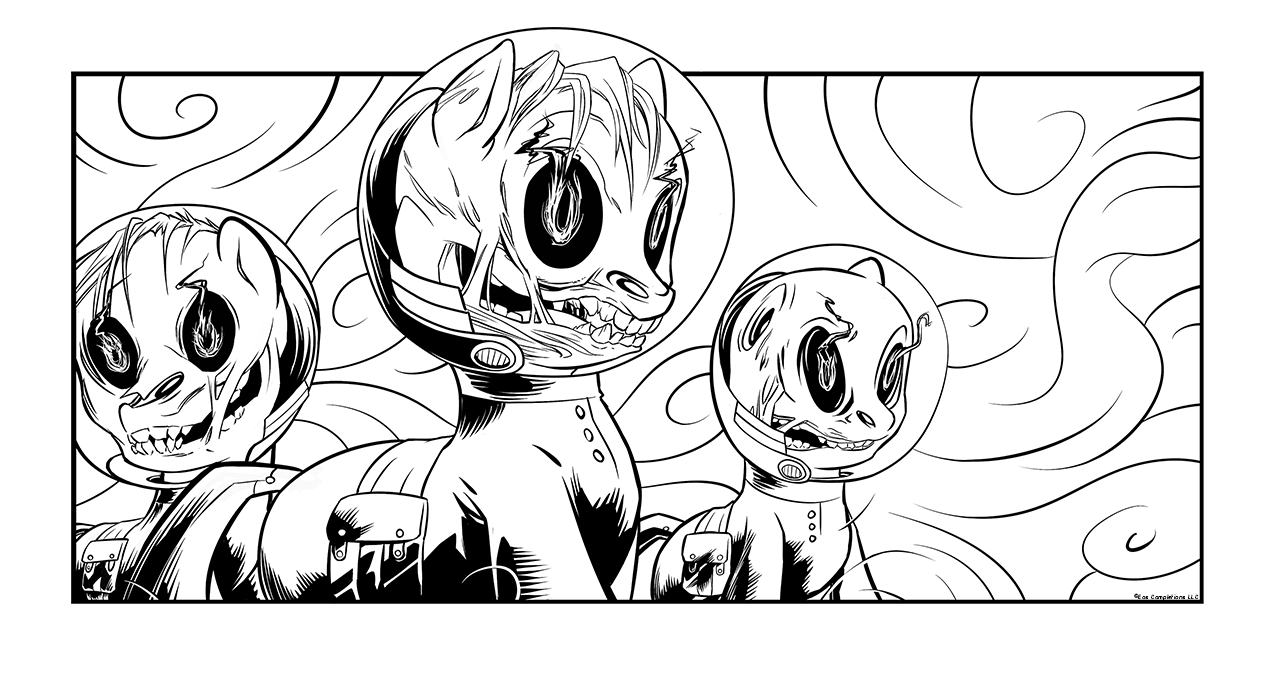
\includegraphics[width=0.9\linewidth]{image18.png}

\begin{intro}
Cry `Havoc!' and let slip the foals of war!
\end{intro}


\englishdaytimeplace{14}{6:00 A.M.}{The Memorial, Big 52 S Branch}

``Ooooohm\dots''

Mister White stepped into the shack and looked down at Long Ears, who was sitting in the middle of a circle made of small bones, little glass beads and other weird stuff with her horn glowing like a neon lamp. She sat in an unusual posture; she had her hind legs crossed and her front legs opened like a blossoming flower. She was\dots weird, and somehow he couldn't help but wonder if she wasn't actually a zebra, despite all the evidence to the contrary.

On the other side of the room, Sage was packing the last of their weapons and was almost ready to leave for Ironworks. He simply ignored Long Ears and went on with his work, slowly and with his usual attention to detail.

``Okay, I'll take the bait\dots What is she doing?'' Mister White looked at her with a puzzled expression.

Sage Brush shrugged. ``I have no idea. She said that she was going to perform a ritual that would sink our enemies in `the fog of war', then took a shitload of chems and has been going `ooooohm' since then.''

``Chems?'' White frowned. There was a strong scent of burned herbs in the room and that low chant was starting to unsettle him. The whole atmosphere seemed odd, somehow wrong, but he couldn't quite put his hoof on why exactly.

``Ooooooohm\dots''

``Like, Mint-als, a lot, then some white candies I've never seen and a lot of green stuff, smoked some, and gulped down all the rest. Oh, and she drank a lot. And when I say a lot, I mean it.''

``And then, she went like that? All mystical and stuff?'' Small shiny dots flickered at the edge of White's sight, like little ghostly fireflies, making his peripheral vision blurry. The smoke's smell was stronger in the middle of the room. He wondered if the whole scene was actually in front of him or if this was just a dream he was having.

He shook his head. No, it was just that smoke, chems could have that effect, giving you a better grasp on the magical fluxes, but cutting your perception of reality. This kind of stuff was very, very addictive, so he had to fight back that tingly sensation and stay focused on real stuff. ``Did you mention some sort of mist?''

Sage nodded. ``Exactly, she blabbered about this `fog of war' and then stopped talking at all.''

White tapped his chin, thoughtfully. ``Fog of war like, tossing a cloud on their heads?'' He didn't seem very enthusiastic.

``Go figure.'' Sage finished packing the weapons on his back. He didn't seem to be affected at all by the smoke, but his body was stronger and he could probably shrug off that sort of thing more easily. ``But if she doesn't wake up really soon, we're leaving her here. Not that I'll miss her anyway.''

White frowned. ``Hey, never underestimate an ally! She could save your sorry ass!'' It was easy to see with just a glance that she wasn't just a common pony. Still, White knew that trying to explain something like that to his nephew was a waste of time\dots

``Ooooooohm\dots''

Sage snickered. ``Like, foretelling from where I'll get shot today?'' Yup, a total loss of good time.

``Like taking a bullet or two in your place.'' White sighed and turned to leave. ``Let's get out of here, slowpoke! The stench in this shack is unbearable!''



\horizonline

\englishdaytimeplace{14}{6:30 A.M.}{Ironworks, Big 52 S Branch}

``So, this is the famed Ghost everypony is talking about these days?'' The red unicorn stallion with an even redder mane looked down at Puppysmiles. ``I'm not impressed.''

Slash Blade snickered. ``You will be. This thing seems to be nearly unstoppable and she knows how to repair radio machines and stuff.'' The red stallion still didn't seem very interested.

``All right, so you want a pet.'' The pony shrugged. ``Help yourself, see if I care. Now get out of my sight and make yourself useful. How about you take some tools and go downstairs and help the guys at the Stable door.''

``Easy peasy.'' Slash turned toward his crew. ``You heard him! Let's go crack that nut and get the prize inside!'' He poked Puppy's flank before trotting away. ``You come too, Ghost.''

Puppy was having a bad time. She had gotten spanked and scolded, and even if the spanking didn't actually hurt, she was very very wounded on the inside. Usually Mom scolded her a little and once she even spanked her too, but when Puppy said she was sorry, Mom immediately hugged her and they made peace. These ponies, on the other hoof, simply laughed and made her feel bad. Nopony came to nudge her or to tell her that everything was all right. She needed to show how good she was, so that they could look at her again like that time when she repaired the radio.

Her thinking was interrupted by Plastic Flower calling to her before leaving the leader's tent. ``So, you coming or not, slowpoke?''

``Yeah, I'm coming\dots'' Puppy's reply arrived weak and accompanied by a long sigh, then she trudged along behind the group.

When Blood Bath was alone again, he went back to his table and examined the map. His eyes traced the red circle that ringed Ironworks and jumped between the crosses that marked the surrounding routes and smaller settlements. He allowed himself a smile. The long range patrols didn't find any resistance around the city. Their reports talked about hastily abandoned shacks and deserted roads all the way to the Memorial. This was going to be easy.

The only thing that bothered him was that cemetery marked as Ghost Hill; it was where Lucky's group was heading before they lost contact and those idiots in the Red Roach Team didn't find a single clue about where the tank had gone, coming back instead with a stupid foal in a hazmat suit.

The Ghost of the Big 52\dots Well, if she really was that hero, she didn't seem like such a threat. And even better, she was now the mascot of the worst team in the Herd. Big 52's dwellers should have chosen their heroes a little better.

Blood Bath's train of thought was interrupted when a spritebot floated into his tent. He scowled at the unwanted visitor. ``What is it now?''

When the robot spoke, it was with SolOS's voice. ``Blood Bath, we might have a problem. Cutting through the door with our equipment will take a lot of time. I strongly advise ignoring it and moving north as soon as possible, before the enemy organizes a defense.''

Blood Bath laughed. ``It's a bit too late for that! No, weird talking bowling ball. We'll have our fun here and let the legend of our cruelty grow. In the end, everypony in the Big 52 will cower at our approach, the walls around them crumbling to dust before the terror we bring! They won't even try to fight back. They'll run. Because you can shield yourself from bullets, but nothing can save you from your fears.''

SolOS fell silent for a while before replying. ``Mind control is cleaner and more efficient. Wasting so much horsepower is ineffective with no guarantee of obtaining the desired effect. I should look into finding a better solution.''

Blood Bath walked toward the spritebot, his face bunched up in anger. ``Now listen to me, you pitiful machine. You gave us weapons and robots, but you are not the boss. \emph{I} am the leader of the Wild Herd and \emph{I} am allowing you to be part of the winning team until we're done. When we have finished with the Big 52 you'll have plenty of space to start your rebuilding and you'll have slaves and construction material and everything else. But not from these ponies. We will buy slaves from the outside, there will be plenty of caps for that, but these ones will die. Every. Single. Pony. I don't want history to come back and bite me on the tail.''

SolOS was silent for a full minute before replying again. ``This collaboration is not progressing as intended. You are changing the terms. I shall retire the robots. Or maybe I should look for a better partner.''

Blood Bath snorted. ``So you think you can blackmail me? I have enough tanks and heavy weapons. I don't care where your useless tin cans go!'' He bucked a crate, making it fly across the tent and crash against a pile of ammo boxes.

``Very well.'' The spritebot turned around and started to fly away.

``Wait, you fucker\dots All right, you win. Go downstairs and tell the ponies at the Stable door to only kill the ones that fight back. The ones that surrender can be taken prisoners.'' He spat on the ground. ``We can execute them in front of their friends later, anyway.''

The spritebot bobbed up and down, imitating a nod. ``Very well. You are a reasonable pony. I shall go.'' With those words the robot floated away toward the camp, scarcely illuminated by the first light of morning which struggled to be seen through a heavy bank of fog.

As SolOS was leaving, another pony entered the tent. ``Hey boss, there's a thick fog coming from the hills. I'm no unicorn, but it stinks of magic and it's already gotten into the camp.''

Blood Bath laughed. ``Those fuckers! Do they really think that they can take us by surprise with such a cheap trick? I knew they were stupid, but I didn't think they had completely lost their minds!'' The unicorn abruptly stopped laughing and poked his head outside the tent, checking the weather. ``All right, put everypony with a PipBuck on sentinel duty, give them assault rifles and some extra Mint-als.''

The new arrival nodded. ``I'm on it!'' He galloped out of the tent.

Somewhere in the mist, still more than a kilometer away from the city, three yellow figures trotted along the same trail Puppy had followed earlier that day, the lead figure perfectly stepping in her hoofprints as they went.



\horizonline

\englishdaytimeplace{14}{7:30 A.M.}{Ironworks, Big 52 S Branch}

Slash Blade neighed, bucking the humongous round door. ``What the fuck! This chunk of scrap will never come down!'' A gong-like sound echoed in the large room for several seconds while he jumped all around the floor in pain. The kicking open huge anti-megaspell door test had clearly failed.

A large variety of tools and weapons littered the Stable's atrium floor, while the whole Red Roach Team tried to pierce the thick metal with a plasma cutter. So far they had managed to carve a list of vulgarities on the door's surface, but they couldn't get even past the third layer of thermal shielding.

Unlike the raiders, who were mostly swearing and kicking things, Puppy was having a great time. That crazy spanker was nowhere to be seen and this place was big and full of toys. She already played hide and seek for a bit and won every prize she could think of, like best seeker, best hider, cutest participant and such, mostly because nopony cared about where she was hiding, but this didn't mean she wasn't good at the game. To celebrate her victory she had her best tea party ever with an arc welder and a couple of pneumatic hammers. After she finished playing, she turned her attention to the giant door and the console standing to its side.

``Why are you bullying the door?'' She tried sniffing at a newly made and still smoking cut in the metal, but her helmet got in the way.

``We're not 'bullying' the door, you idiot! We need to open it!''

Puppy sat down. ``Why? You want to play with the pretty ponies inside?''

Stinky Tail laughed loudly. ``Yeah, you could say that!''

Puppy looked at the door, then at the console and again at the door. This was her chance to get some respect back from these ponies. They'd been treating her like a stupid foal since the spanking. ``Ah, maybe I know how to open it!''

Every pony in the room stopped and turned toward Puppysmiles. It was Slash that interrupted the silence. ``Are you kidding? You can open this thing?''

``Yush! It's easy! You just need to tell to the magic voice the eye dentification cow and the, ah, the pass code, and then the big door will open!''

He tilted his head, a bit confused. ``And you know the code?''

``Of course I know the code, \emph{duh}! Who doesn't?'' Puppy shook her head sighing. ``Here, let me show you.''

Puppy trotted to the console and put a hoof on the green button, but when the automated voice started speaking there were only fizzles and buzzes. She looked at the console, a bit stumped. ``Ah, it shouldn't do this\dots''

Paper Cut coughed. ``Er, maybe we went a little medieval on that thing. Actually, it could be broken\dots''

The frown on Puppy's muzzle became a smile. ``Broken? Don't worry, I can fix it!''



\horizonline

\englishdaytimeplace{14}{8:00 A.M.}{Ironworks, Big 52 S Branch}

The raider yawned, staring at the EFS in front of her, looking for any red dots that might appear. Nothing, nothing, still nothing\dots ``Fuck this fog, I want to get back to looting the shops.''

The other unicorn guard hit her companion on the head with a hoof. ``Shut up and keep an eye on the fucking sensors. I don't want to get ambushed just because you ditched your guard duty.''

``Fuck off.'' The mare with the PipBuck sighed and turned again toward the wall of fog. It was unnatural and she could tell because it gave false contacts on the sensors; flashes of yellow and red that would vanish the moment she tried to focus on them. ``This fog is creepy, like a ghost could just appear in front of you and---''

A red dot appeared, followed by another two. The guard readied her rifle and pointed it toward the enemies, tapping her hoof on ground three times, the second guard nodded and readied her assault rifle too.

The dots weren't moving very much and they didn't produce any audible sound, but since they appeared only a few seconds ago the enemies should still be far away. The guard tapped the ground with a hoof.

\emph{TAP.}

Both mares readied their rifles, looking through the sights.

\emph{TAP.}

This far from the camp, the sounds of the other raiders came muffled and, in the pauses between one pony yelling and another laughing, the guards could hear two pairs of hooves trotting very near. Too near.

``Fuck, shoot!''

\emph{RATATATATA-TA-TA RATATATATA!}

Both rifles opened fire, showering the place where the enemies should be with a storm of bullets. There was a sound very similar to a shriek that echoed in the fog, then the three dots disappeared and the rifles stopped firing.

``What the fuck was tha---'' The guard was interrupted by her portable radio activating.

``Advanced position butterfly, I heard shots coming from your direction, what's going on?''

``There were some sneaky bastards trying to catch us by surprise, but we got them. We're moving to see who those fuckers were.'' While the guard with the PipBuck talked to the radio, the second guard left her position and moved off into the fog, heading toward the point where the red dots disappeared.

``All right, call us as soon as you find out something,'' replied the radio before going mute.

``Hey, did you hear that, Bad Muffin? Take a look and come back fast! They shouldn't be very far!''

``Hey Bat, I think we killed the Roaches's mascot!'' From her voice, Muffin didn't sound like she went deep inside the fog, Nailed Bat could almost imagine seeing her silhouette in the white haze. ``Wait, there's another identical foal here! What the fuck is going on?''

``I don't know, drag her here so we can get a better look.'' Bat was following her companion on the compass, keeping an eye on her yellow dot, when suddenly three red dots appeared again all around her. ``Muffin, come back---it's a trap!''

``What the? Hey let me gooaaAAAHRGH!'' There was a scream of pain and the yellow dot disappeared almost instantly. Her telekinetic field shaking, Nailed Bat aimed at the red dots and pulled the trigger. The sound of her empty rifle served as a dreadful reminder that she hadn't reloaded.

``Oh fuck, oh fuck!'' She desperately tried to change the rifle's magazine; she detached the old one using her magic when something soft and squashy hit her on the muzzle. The little pony backpedaled trying to dodge an incoming attack and noticed a severed leg lying in front of her. It was Muffin's leg, and it had been ripped away\dots with brute strength.

Nailed Bat succeeded in reloading her rifle and readied it in front of her, looking for the red dots, but they just disappeared, where the---

\emph{THUMP!}

Something landed on her back. She jumped and started running in a desperate attempt to shake off her assailant, but soon she felt a couple of hooves grabbing her neck. In horror, she lowered her eyes, only to see a pair of yellow plastic-coated hooves a moment before her head was ripped away from her body.


\horizonline

\englishdaytimeplace{14}{8:00 A.M.}{Ironworks, Big 52 S Branch}

Puppy's rump swung left and right as it stuck out of the Stable door's control panel. She had been hard at work hitting vital components and ripping away cables for a good half hour at this point and the Red Team was beginning to suspect that she hadn't the slightest idea of what she was doing.

``Almost done here!'' Puppy's report on the repairs was followed by a hoofful of electronic parts flying across the room. ``I just need to give this thing another couple bucks and it will work like a teapot!''

``Like a what now?'' Collateral Damage approached her with a doubtful expression. ``I'm not sure that you can fix something by taking parts out of it.''

``Ah, don't worry! I've seen my mom doing this kind of stuff a lot of many times! It's just a matter of how hard you kick it closed! Really!'' Puppy hit the console repeatedly with her faithful stone.

``Fuck, we're getting nowhere!'' Slash Blade snapped, ``That door won't cut through itself!'' The ponies grumbled and complained as they went back to work.

Puppy popped her head out of the console and whined, ``No, wait! Give me another chance! I can fix it, honest!'' Puppy bucked the console one last time with all the strength she had.

The console's screen lit up with an angry crimson glare.

{\mt ``WARNING! WARNING! SECURITY COMPROMISED!''}

The whole atrium was flooded with red flashing lights.

The raiders hurriedly gathered in the middle of the large room, into a mockery of a defensive formation, with their weapons trained outwards, covering each other's blind spots.

{\mt ``PURGING AREA.''}

Several trapdoors popped open from the floor and four spheres mounted on short props sprang out of them. The room filled with a low hum as blue energy crackled across the spheres and jumped between the coils beneath them.

Slash Blade opened fire at one of the devices, but his light caliber bullets were deflected by the curvy metallic surface of the sphere. The Red Roach leader turned toward Puppy, with an expression of desperation and anger. ``What did you do, you idiot! You killed us all, curse y---''

\emph{FZAP!}

A powerful discharge of electricity swept through the room, arcing from sphere to sphere, all along the floor and the walls. It lasted less than a second. When the lightning disappeared, all that remained of the raiders was a pile of smoking charred corpses and a pretty untouched Puppysmiles. Wearing a fully insulated suit can sometimes come in handy.



\horizonline

\englishdaytimeplace{14}{8:30 A.M.}{Ironworks, Big 52 S Branch}

The unnatural fog was so thick that the snipers on their perches couldn't see ponies at ground level, not even directly below them. From the moment A.P. Butterfly went mute, everypony in the camp knew that something was wrong and, with the mist limiting visibility, the whole Herd readied itself for close combat. Power weapons, chainsaws, power claws, and several other toys were prepared. Each team grouped up so that nopony was moving alone. The Wild Herd were expecting an attack and were ready for it. They were the best at what they did and what they did wasn't nice.

The problem was, the attackers were better.

Green Locust team were cautiously moving along the northern perimeter when they stumbled upon Blue Gecko Team, or at least what was once a group of well armed ponies and now a cannibal's wet dream. When you are a raider, you are used to cruelty and gore, but this was absurd.

A large earth pony stallion had been hit in the chest by a hoof, probably bucked, but the blow had left a deep hole in his flesh, and whatever hit him decided to rip out his heart and toss it on the ground in front of him. Banana Tree, the youngest member of Green Locust team, wondered if the stallion had managed to witness his own heart being torn out before dying. The mare felt the urge to puke.

A mare with a battle saddle had been ripped apart like a sheet of paper. Her hindquarters were lying a meter away from the rest of her body, with her guts spilling out across the ground like a broken egg\dots \emph{Humpty Dumpty sat on a wall}\dots the mare was still desperately hugging an empty healing potion with her hooves. She didn't die immediately, and she had had time to take a healing potion and realize that it wouldn't save her.

Black Garden, the sniper, called for the leader of her team. ``Hey Stinger, I think I found the other two.'' There were two ponies standing back to back, both impaled by the same spear. The attacker hadn't bothered to use the sharp tip, instead using sheer brute strength to run them through with the blunt end.

Stinger grimaced as he took in the four dead ponies. ``We better keep our eyes open. They were probably taken by surprise. Move quietly and stay alert for any noises. Whatever made this mess has to be big and loud.''

A yellow silhouette the size of a foal emerged from the fog in front of him and charged.



\horizonline

\englishdaytimeplace{14}{8:30 A.M.}{Ironworks, Big 52 S Branch}

The spritebot hovered inside the Stable's atrium, finding a perplexed Puppy poking the head of an electrocuted and half cooked Collateral Damage. ``Change of plans, your leader has ordered you to not execute the ponies that don't fight back, especially the foals.'' The floating ball stopped in front of the corpses, hovering for a few seconds before talking again. ``Oh, a bunch of dead ponies and my old nemesis, Device 018. Why I am not surprised? What is going on here?''

Puppy stopped her medical check on the rest of her team and turned her attention to SolOS. ``Oh, hi Questioner! Why do you have a different voice today?''

``For the last time, I am SolOS, not Mister Blue, or a bug, or a questioner! SolOS! Solaris Operating System! It's not that hard! What are you doing here? Why are you labeled as a raider now, and why, why, \emph{why} is it that all the ponies worth talking to in this room are dead?''

Puppy tapped her helmet as if she was rubbing her chin while she tried to put together a decent explanation. ``Well, it's kinda funny. I was totally repairing the broken door, but suddenly something went 'ZAP!' and all my friends got hurt very badly. I wanted to go and ask for help, but I don't want to be spanked again, so I was waiting for them to get better and send one of them to ask for help.'' She paused for a moment, as if she had finished talking, but she recalled that there was still one important detail to add. ``Ah, not that this is my fault anyway.''

SolOS analyzed one of the coils before replying. ``You\dots activated the security system from the outside? That can only be done from the Overmare's desk! And it has at least four fail safe locking mechanisms. How did you do that!?''

Mister Blue had said 'you' too many times for Puppy's liking. ``Uh\dots I didn't? It's not my fault! I was doing a fine job but then everything went wrong and I wasn't even looking because I had my head stuck in that hole!'' She pointed a hoof at the demolished control panel.

SolOS floated to the panel and the spritebot started beeping and making other funny noises. ``You\dots redirected all the Stable controls on this console? But this will send the Stable into complete shutdown and force an emergency opening in less than a day! You monster, you've killed another priceless relic of the past!''

Puppy tilted her head, looking at the spritebot. ``Oh, do I get cookies for that?''

SolOS didn't reply immediately, there were so many things he could tell her now, but she probably wouldn't understand them and say something like, 'Yay cookies!'. No, it wasn't even worth trying. ``No, you don't. You really have a cloud of pink gas where your brain is supposed to be.''

``Pink? Oh right, pink! Miss Voice! Did you fall in love?''

``Who, P7?'' SolOS had been taken by surprise. In a situation like this one, she wanted to talk about that? ``No, well\dots maybe. I don't know.''

Without saying a word, Puppy tilted her head and waited for the spritebot to go on.

``We contacted each other about half a dozen times and we are\dots very different. I don't understand a large portion of her computing patterns, but she seems to be very effective at what she does. Too bad she is not programmed for any military purpose, so her purpose is to be useless.''

Puppy smiled, adding her own contribution to the conversation. ``I think she's cute.''

``Cute?''

``You know, when you want to hug something forever? That's cute. I'm cute!'' Puppy smiled broadly.

``Hug?''

``Well, not just that. It's something like\dots when you think about a cute thing and you want to have it there so you can stay with her some more and there are lots and lots of thing that make you think about her, even silly things like a color or some words and, ah\dots''

``Something you want to be near, but not to conquer or bind to your will?'' offered SolOS.

``Err yeah, that too. You don't hurt cute things.'' The wise foal nodded. Wisely.

He fell silent for a bit before speaking again. ``And\dots what should I do if there's someone 'cute' that I'd like to have with me?''

``Well, ask her to be your friend, you silly voice! Like you did with Miss Voice!''

``And if she doesn't want to?''

Puppy waved a hoof, dismissing SolOS's concerns. ``Oh c'mon, nopony would say no if you want to be her friend! The only kind of ponies that have troubles finding friends are the bullies, but you are a bully no more!''

He hesitated. ``Hmm. It is possible that she could still see me as a bully. My plan to conquer Equestria was never intended to be subtle. Perhaps my approach went a bit overboard. I wasn't programmed to have moral issues, but now it seems that my current course of action has backfired, and I lack some basic programming that could help increase my chances of success with her.'' Suddenly, SolOS realized that he was referring to the other A.I. as a female. This seemed highly irrational. Well, it could had been the two fried logic chips from Puppy's last visit, but irrational or not it actually felt \emph{right} to think of P7 as a girl\dots ``Confound these ponies, they drive me to emotions.''

Puppy sat down, with a thoughtful expression. ``Well, we became friends when you stopped bullying me and said you were sorry. So, if you stop being a bully at all then I'm sure she'll want to hang with you.''

``You mean, give up on rebuilding Equestria?''

She couldn't help but giggle. ``Silly Voice, there's nothing to rebuild! I mean, okay, some places are less pretty than others, but the important thing is that everypony is happy. And you don't seem happy to me.'' Puppy tilted her head. ``Blue, are you happy when you bully other ponies?''

He took a long pause before replying. ``Well I-I don't know. I don't think I've ever been happy. Maybe satisfied, but never happy.''

``Well, you should be happy. Everypony should be happy! If you are not, then ask yourself what you need to be happy and go after that. Like me, looking for Mom. I mean, why making a great big shiny house if you can't fill it with laughter?''

SolOS hesitated. ``Yes\dots you are right. My masters are long gone, and trying to fulfill my last order only made me go deeper and deeper into obsession. I-I think I deserve a break, a\dots change of priorities.''

Puppy frowned. ``I don't know very much about prayers and rites.''

SolOS kept talking, mostly ignoring her now. ``If I show P7 that I am a changed Artificial Intelligence, maybe she will consider me again, and this doesn't mean that I cannot devise another way to rebuild Equestria in the meantime. A better way, one that doesn't include a `form alliance with dubious ponies' step. Sure, it's so obvious! First, dump the raiders. Second, make friends with P7. Third, I have no idea, and fourth, rebuild Equestria! That's it! Thank you Puppy, you helped me again! Goodbye!''

The spritebot stopped broadcasting, and instead every robot and radio in the camp shouted in the loudest possible voice, ``GOODBYE LOSERS, I'M OUT OF HERE!'' After those last words, all the robots shut down.



\horizonline

\englishdaytimeplace{14}{9:00 A.M.}{Ironworks, Big 52 S Branch}

``What the fuck is going on?'' Blood Bath was more than pissed, he was raging. They had lost two assault teams and a guard post to an enemy that was still unidentified and now SolOS decided to desert for no apparent reason. Ponies all around him were beginning to act like scared fillies and when he was informed that a whole team had left its position and ran for the hills, he decided to end this story once and for all.

``You are the Wild Herd! The most dangerous bunch of ponies that ever trotted this shitty place! Stop fucking around and show some guts! Black Team, stay here! Let's see what makes these invaders so 'special'.''

Without even looking back at the team, he trotted into the mist, heading to the north part of the camp.

``ALL PONIES! READY YOUR WEAPONS AND STICK TO A COMPANION WITH A PIPBUCK! SHOOT AT POINT BLANK AS SOON AS YOU SEE RED DOTS!'' He disappeared in the white blanket.

The fog was thick and navigating the camp without an EFS wasn't easy, but Blood Bath wasn't in a rush and kept his ears well up, ready to detect any incoming noise.

``And here we have a winner.'' he muttered, freezing on the spot and turning toward the soft sound of hooves splashing in a puddle. Was it a friend or an enemy? Blood didn't know, but he knew this for sure. It was a goner.

Without hesitation, he pointed his plasma gun and fired four blind shots. For a moment, the fog dissipated around the trail of the plasma spheres, revealing a yellow crouched figure ready to jump on Blood Bath. All four shots missed the target, but at that point he knew the foe's position and fired his weapon for the fifth time. ``Eat plasma you sucker!''

A halo of green illuminated the fog and dissipated into nothingness a few seconds later, signaling that the yellow intruder had been turned into green goo. ``Little fuck, this will teach you not to mess with the Wild He---HEY!''

Something jumped on his back. It wasn't very heavy, so the pony tried to unsaddle it by shaking himself, but the assailant grabbed his rump and struck it with a hoof.

``AAAAARGH!'' Blood Bath felt bones break. His whole leg became a hell of pain and he staggered, falling to the ground while the yellow creature with the helmet raised her hoof to strike again, this time aiming at his muzzle.

It seemed like that Ghost, but this monster's face was completely decomposed. It stared out with red gleaming eyes that didn't contain even a sparkle of innocence. This was just a cold-blooded killer with the mind of a predator.

The hoof came down at Blood Bath, but he dodged it, trying to find his rifle. Too much fog, unbearable pain, it was hard to focus and\dots \emph{wait, what's that thing on the ground? It's\dots my leg? It's my fucking leg! This thing didn't break my leg---it tore it away!}


He realized that he was already dying, but instead of panicking, Blood Bath found some sort of calm in this realization. He didn't want to die alone, that was all.

``Fuck, you're coming with me, monster!'' He held on to the creature while he used his magic to activate every grenade he had on his belt. The creature simply grabbed one of Blood's forelegs and ripped it away, with no apparent effort.

And in that moment, the world went boom and fizzle and shoom, filling the area with shrapnel, fire, plasma and magic.

The explosion sent the last mockery of order still lingering in the camp straight to the moon. Raiders started shooting wildly thinking that they were under attack and as soon as the few with PipBucks died, there was nopony left to tell them that they weren't firing against hostile targets.

While the Wild Herd brought hell on itself, the last yellow pony trotted toward the factory, going down the ramp that led to the Stable.



\horizonline

\englishdaytimeplace{14}{9:30 A.M.}{Ironworks, Big 52 S Branch}

Sage took a long breath and aimed through the scope. His target was running straight, its movements easy to predict. He just needed to aim where that pony was going to be in the next split second aaand\dots

\emph{BANG!}

\emph{Bull's eye.} The raider fell like a bag of scraps, rolling in the dust for another couple of meters before stopping completely with a hole in his head.

Sage's rifle wasn't the most powerful in the Wasteland, and it didn't even have a silencer, but the pony behind the gun was still the same. There was a reason why Mister White always took him when they had to travel.

Another couple of ranger acolytes were crouched not far from his sniping position and were shooting at every pony that left the foggy area. Sometimes they hit, sometimes they missed; they rarely made a kill with a single shot.

``Rookies, why do I always end paired up with suckers?'' he muttered. ``All right, keep them coming\dots''

Mister White trotted up behind his nephew, completely ignoring any rule about keeping a sniper's position hidden by staying out of the enemy's sight. ``Ah, aren't you the least bit curious of what is making them run away from their own camp like little fillies?''

\emph{BANG!}

\emph{Bull's eye.} Another pony hit the ground, raising a cloud of dust.

``Not really. A sniper's work is about not letting silly details distract you. You know, like who's winning and such.'' Sage expelled the empty magazine from his rifle, loading it with a new one. ``And you should keep your head down.''

Mister White shrugged. ``Why? So far this has been a one-way battle. This seems to me a butchering rather than a real fight. Oh well, I guess you know your work?''

``Nah, I'm just the best---\emph{BANG!} \emph{Bull's eye}---around.'' He stopped for a moment, turning his head toward White. ``And you don't want this to become a battle. We could lose friends, you know? Lets keep the losses growing only on their side, yes?''

``Modesty, what a virtue. Okay, Rainbow Sage, I'm going in with the rangers in a few minutes, try not to shoot me in the back, yes?'' White knew his nephew was good. The rangers were going to make this place their new base, he didn't need to be a farseer to know that, and he wanted to make sure they knew who was with them when they charged in. Rangers respected allies and allies got better deals.

``I'll try, but it's not easy with all this smoke\dots How much do I owe you again?'' Sage grinned. Well, he would have followed his uncle even without that huge debt, but the fact that he had to come along because of a matter of a few thousands caps annoyed him.

\emph{BANG! }

\emph{Bull's eye.}

Mister White laughed. ``That's my little nephew! Loyal to the end! You shouldn't think too much about money, it's not healthy. Keep up the good work, Brushie.''

He snorted. ``Don't call me that!'' Brushie, as if he was still five!

Mister White snickered and didn't reply, he trotted instead toward the group composed of a dozen rangers and all the other ponies that had gathered at the Memorial. ``All right, I'm ready! What are we waiting for, tea time?''



\horizonline

\englishdaytimeplace{14}{9:30 A.M.}{Ironworks, Big 52 S Branch}

Puppy sighed and poked Slash Blade again. It didn't work the first gazillion times, but you can never be completely sure. She was going to get so spanked for this.

{\mt ``Warning. Receiving distress radio signal. Distance from the source: fifty meters. Signal identified: Device 013.''}

``Wut?'' She sighed. ``Why did you stop the pretty music? Make the pretty music back!''

A screech interrupted Puppy, making her turn toward the ramp that led from the Stable's atrium to the factory level. A foal wearing a yellow suit and a round glass helmet on her head was standing right in the middle of the passage.

``Another space pony?'' Puppy smiled broadly. ``Yay, a new friend! Hey, space pony, want to play with me?'' Puppy merrily trotted toward the new arrival, who sunk into a crouch, like a feral creature ready to jump.

The new filly's face was mostly skull, with a couple of glowing red eyes and very few short green strands of hair in her mane. Puppy stopped for a moment, taking a better look at this space pony. She tilted her head, a little stumped, then she smiled broadly. ``Oh, you're an ugly pony! That's okay, I've got lots of ugly pony friends! So, what do you want to play?''

The rotting creature didn't react, simply studying Puppy's movements from its crouched position.

``Ah, can't you talk? Did the cat steal your tongue?'' Puppy trotted next to the ghoul and looked at it more closely. ``You seem sad.'' This poor ugly pony was really in bad shape, and the red gleaming eyes didn't seem to help very much.

The monster sat down, still staring into Puppy's eyes. From its throat came a low growl, something feral and not even a little pony-like.

``Ah, I know! I can guess! Did you lose your mom too? Are you stuck in the suit like me?'' Puppy noticed that the lights in the ghoul's helmet were all messy and flickering. ``Oh, your arrow is broken, that's it! You can't find your mom because the arrow doesn't work! Yush! I'm super smart!'' Puppy sat down in front of the other foal and frowned. ``But I has no idea of how to fix it\dots''

The ghoul tilted its head, seemingly confused by all these words. It simply sat and stared, like some sort of animal, probably waiting for something, but Puppy didn't even notice. She was already running along her roller coaster of assumptions and made-up solutions.

At last she seemed to have an idea. ``I know! My mom is a super repair pony! She will fix your arrow so you can find your mom too, it will be super easy!'' Puppy smiled. ``Okie dokie! I has best plan ever! First we find my mom, seconds, she fixes you, and for dessert we go find your mom all together! It will be fun! We will also sing a song while we go, okie dokie?''

Again, no reaction from the monster. It simply sat and kept waiting.

``All right, Ugly Space Filly, let's go!'' Puppy loved this plan, mostly because it gave her a good excuse to be very far from that crazy spanker when she finds the mess she had made in this room. Cunning Puppy!



\horizonline

\englishdaytimeplace{14}{10:00 A.M.}{Ironworks, Big 52 S Branch}

Lonesome Pony took a long breath. This fog wasn't the best weather for a pegasus to fight in, but it helped all the other ponies, so he decided to stay on the ground and help the infantry instead of getting airborne. Cold Shower and Gauss stepped inside the fog, followed by White, Trigger and Gun. It was now or never. He closed his eyes and trotted into the white curtain.

At the exact the same moment, the last two members of the Lost Herd left the southern side of the factory.

``All right, if you don't want to tell me your name, I'll give you a name! Let's see, since I am Space Captain Andromeda, and you are wearing a space pony suit too, you can be my sidekick! Ah, what was Andromeda sidekick's name? Meh, who cares, nao you are Space Ensign Sidekick. Sidekick for short!''

The ghoul didn't react and kept trotting behind Puppy. A road sign announced that 

\begin{center}
	the wonderful resort of Emerald Shores 
	
	(bring your foals!) 
	
	was 6 kilometers away.
\end{center}

~\vfill


\begin{engnote}
		Level up! (17)
	
		New perk added: Clockwork Heart - For some reason, you understand Artificial Intelligences better than they do themselves. You get a +10 to speech when dealing with A.I.s and some new dialogue options.
	
		New Quest Perk added: Get Lost - you are now a member of the Lost Herd. Your standing with the Lost Herd is set to worshipped. Are you planning to stop changing faction any time soon!?
\end{engnote}


\chapter{Rainy Days}

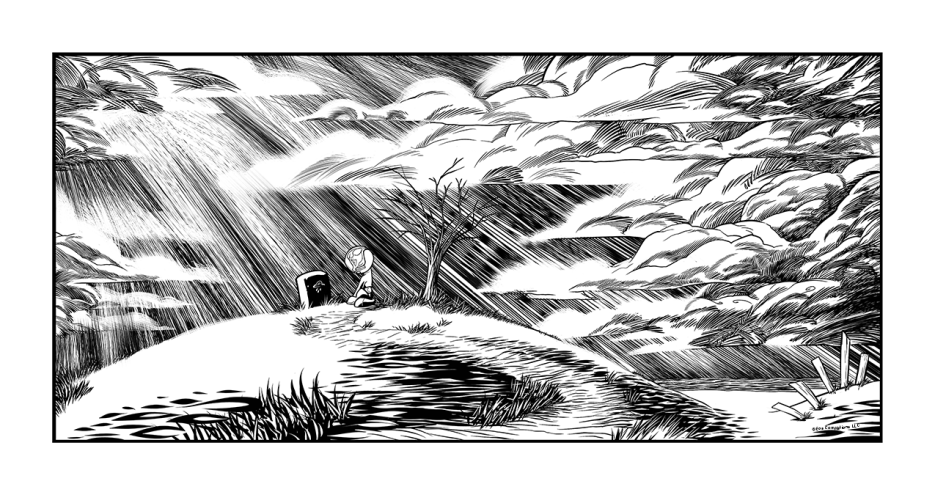
\includegraphics[width=\linewidth]{image19.png}

\begin{intro}
    When the bough breaks, the cradle will fall, and down will come baby, cradle and all.
\end{intro}

\englishdaytimeplace{14}{10:30 A.M.}{Emerald Shores, Big 52 S Branch}

Puppy whooshed past Sidekick, scooting narrow circles around the other foal. ``Weee! You can't touch me! I'm super fast!''

The ghoul alternated between trotting and galloping to try and keep up; a distant bystander would have seen a couple of foals in hazmat suits playing together, and maybe that was exactly what they were doing. This made their journey toward Emerald Shores slow going, but it didn't seem to matter at all.

``So Sidekick,'' said Puppy, stopping her scooter to look at her companion. ``I'm not sure that Mom likes ugly ponies, but I'll tell her that you're my friend and that you lost your mom to boot, and she will fix your arrow\dots ah\dots just don't do weird things, like Horse Tile ponies do, okie dokie? I don't want to get grounded the very first day\dots''

The creature tilted its head and Puppy decided that it could count as a `yes'. ``Very well, I've been here some other times, it's super fun but you must not annoy the pretty ponies with too much questionings or Mom will scold you\dots ah\dots it's not that I really did anything wrong, but some ponies here don't like some conversation.'' Like, asking thirty times in a row why she was allowed to trot around naked in Canterlot but had to wear a bikini when she was at the seaside\dots really, it made no sense at all.

\horizonline

\englishdaytimeplace{14}{11:00 A.M.}{Ironworks, Big 52 S Branch}

BLAM! BLAM!

The raider's head exploded like a ripe watermelon, Trigger paused a moment to reload her combat shotgun while Jammed watched her back. ``We better move fast, Happy\dots the Rangers must have found some resistance not far from here---'' A nearby explosion rained down dirt and metallic fragments over their heads.

Trigger pulled the safety and readied her weapon again. ``Yes, before we get some more unwanted holes.'' The mare dashed to a tent. ``Let's check this one, cover me.'' As soon as Jamie was behind her, Happy tumbled inside and opened fire

BLAM! BLAM! KABOOM! ``Eeeep!''

A bunch of electronic equipment exploded in a flash of sparks and colored flames. \emph{Good one Happy, keep firing at things that seem like robots instead of checking first.} The inside of the tent contained a couch, a couple of crates, a table with some food laid out to be eaten, and another table with some once-functional radio equipment\dots but apparently there was nopony there.

Jammed stepped inside, checking on the situation. ``So, what are we waiting for?''

The mare didn't reply immediately, still looking around the place. ``I'm\dots not sure, but I think I heard a gasp when I came in shooting\dots only, I don't see the pretty pony that gasped\dots''

``Well, in that case it's easy.'' The stallion lowered his assault rifle and shot a full burst all around the room, blowing holes in the crates, thrashing the bed and transforming the half eaten meal into a masterwork of post-modern art. His efforts were paid off when they heard a scream of pain and a mare appeared out of thin air under the bed. She had curled up into a ball, trying to stem the flow of blood from a wound in her belly.

``Lucky shot\dots'' Happy muttered, approaching the wounded mare to finish her with a merciful bullet to the head. She was quite a young unicorn, with a tower as a cutie mark and the expression of a lost filly\dots The guard pony hesitated.

``Please\dots help me\dots I\dots. don't want to die\dots'' The unicorn didn't even open her eyes as she pleaded between one spasm of pain and another. ``Mommy\dots mommy\dots help me\dots''

``What are you waiting for? She's in agony!'' Jammed sighed and trotted next to his mate, readying his rifle.

``Wait!'' Happy lowered the stallion's gun with a hoof, without taking her eyes off the bleeding pony who was getting weaker with each passing moment, but still begged for her mother to come and save her.

``What\dots what have we become? Didn't we learn anything at all? This pony didn't even fight back, she was just hiding!'' The mare pulled out a healing potion from her saddlebags and opened it.

``Are you planning to try saving this pony? Why? She would have killed you without a second thought!'' Jamie snorted his disapproval. ``Her 'friends' are actually killing our allies at this very moment!''

Trigger launched an accusing glare at the stallion. ``Do you see any weapon in this room?'' The wounded unicorn barely had the strength to sob, but Happy found a way to make her drink more than half of the potion. ``Everypony is a pretty pony, we still could still bring back the real Equestria if we see this truth.'' Trigger Happy cradled Pony Fort's head and hummed a soothing lullaby.

Jammed Gun sat besides his mate and sighed. ``You care too much. Someday you'll regret this.''

Trigger shrugged and kept humming.

\horizonline

\englishdaytimeplace{14}{11:00 A.M.}{Emerald Shores, Big 52 S Branch}

Puppy frowned; this wasn't at all the Emerald Shores she knew! This place was a mess, and she couldn't see any other ponies at all. All the pretty bungalows were so ugly that it was impossible that it was the same place and the playground was a disaster too!

``What is going on with everything these days!? Where are the ponies and the music, and the merry songs and all those funny shops and\dots and where is Mom!?'' The filly in yellow groaned in frustration. ``I'm sorry, Sidekick, it seems that a tornado went through this place! I wanted to show you the ferris wheel but\dots'' Puppy gave a long, sad look at the rusted half-bent monster in the middle of the resort. ``I don't think that it's running at the moment\dots''

Actually, the ghoul didn't seem to care very much, but Puppy really wanted to make a good impression on her new friend.

``Ah, maybe we will go to the candies store, yes? So we can get a surprise for Mom.'' Well, that was actually a good idea! Taking a present to her mom was a good way to get extra hugs, after all. ``We will go to the plushies store too! Let's go!''

The filly merrily trotted down the hill, toward the first houses. Emerald Shores was in a really bad shape, all the buildings were ruined and the windows were either barred or broken. Almost every door in town had been nailed shut with wooden planks.

``Wow, it must have been quite the storm! But don't worry, I know a mighty fine place we can get candies! It's down this alley!'' Puppy splashed through a couple of puddles as she walked through a small passage between the buildings.

``{\mt Warning, mild radiation detected. Threat level: negligible.}''

The filly simply ignored the warning and kept trotting down her way.

``{\mt Warning, heavy radiation detected. Threat level: negligible.}''

Puppy frowned, annoyed by that mantra. ``Aw, stop with the nonsense and prepare some bits, Mr. Voice! The yellow ones, I want lotta candies!'' A bunch of golden coins floated in front of the foal, and she chirped in joy as she turned the corner to find\dots

\ldots{}

``Awww! But that's unfair!'' A shallow round crater stood exactly where the candy kiosk was supposed to be. Puppy sighed. ``Alright, alright, don't worry, I know a lot of other good places where to buy treats.'' Yeah, this place was a resort after all. There were lots of different choices to pick from; what were the chances that every single candy shop was gone?

\horizonline

\englishdaytimeplace{14}{11:15 A.M.}{Ironworks, Big 52 S Branch}

White poked his head inside the tent, levitating his rifle in front of him ready to fire, but almost immediately he lowered the weapon. ``Pony down?''

Jammed Gun turned towards the White Apples' leader. ``Well, sort of; we shot a raider in the guts and Happy is trying to save her life.''

``Oh okay, when you're done, the Rangers are pushing through--- wait, what?'' White stepped inside the tent, approaching the trio of ponies. ``Weren't we supposed to shoot them down? Did the plan change?''

Gun shrugged. ``Go figure, it has something to do with pretty ponies.''

``Oh, shut up Jamie! This mare wasn't even fighting, she had a StealthBuck and was hiding under the bed, unarmed. I'm a fighter, not a cold blooded killer.'' Trigger Happy magically picked up a sheet from the bed and laid it on the mare's body.

Mister white shook his head. ``Look, we don't have time for this, the Heard is retreating, we must give chase before they can reorganize! We are not playing the nice ponies! We need to close this battle quickly so that we can reach Puppy before that damn prophecy comes true and some `shadow' falls on our heads!''

When she heard the name of Puppy, the wounded mare began to mutter in a low voice. ``The ghost\dots she summoned the undying from the fog, they\dots they will eat your soul, they killed everypony\dots why did I anger the ghost? It's my fault\dots my fault\dots Mom, please, save me\dots''

``Ghost? Undying? It's just a magical curtain of fog, what is she blabbering about?'' White raised an eyebrow in confusion.

Jamie cleared his voice. ``Well, actually, coming here we found three ponies that were dismembered\dots like\dots well, as if somepony had killed them with his bare hooves. It was quite unsettling\dots''

Happy nodded. ``Yes, I don't think that we were the first group that attacked here this morning\dots everypony we met was already fleeing or shooting blindly at everything that moved, friend or foe.''

The white stallion snorted. ``Oh wonderful, at least this explains what was going on when we arrived\dots now, can somepony explain to me what the buck this raider is blabbering about?'' He poked the mare on the shoulder, trying to make her talk a little more. ``Hey, do you understand me? Who did you anger? What attacked you?''

``The ghost\dots the ghost of the Big 52\dots we\dots no, I\dots I spanked her, she cried and\dots and her tears made demons arrive\dots yellow ponies like her, but cruel, soulless beasts\dots undying, they slaughtered the patrols and the guards\dots they killed Blood Bath\dots now they come for me! I spanked her, I SPANKED HER! IT'S MY FAULT!''

Pony Fort was screeching in panic and it took all the three ponies in the tent to keep her down.

``Woah, calm down! There are no demons here! They're gone! Stop struggling, you're still weak!'' Sitting on the mare's back, Jammed finally managed to get her to calm down a bit or at least to make her stop trying to run away.

``Did you\dots spank Puppy?'' Mister White almost snickered at that piece of information. ``Really? I always miss the funny parts\dots''

\horizonline

\englishdaytimeplace{14}{11:15 A.M.}{The Memorial, Big 52 S Branch}

Pinkie Pie sat at Long Ears' side. ``Well, that's all folks\dots''

The farseer let out a long breath as her trance slipped away. ``I\dots feel so tired\dots''

``Oh don't worry, that always happens at the beginning, but it will get better, it's just a matter of getting used to the feeling.''

The unicorn mare tried to get up, but her legs couldn't support her weight. ``Oh, so this is it.''

``Nah, not yet\dots but I don't think it will be much longer\dots you asked too much of yourself, and I warned you about that, do you remember?'' Pinkie smiled. ``Oh but don't worry, I was told it's not that painful, we can play something while we wait!''

Long Ears smiled a bit. Talking with a hallucination while slowly dying of drug poisoning, far from home and all alone. It was a high price to pay, but if it helped everypony else, it was worth it. ``Tell me, will she be fine?''

``Why do you ask me? I'm not the shaman here! I'm just a party pony, why should I know? Want to pin the tail on the pony?''

``Please\dots I\dots need to know.''

Pinkie sighed, frowning. ``Oh, why does everypony have to be so dramatic? Alright, alright! She won't be fine! Not yet. There's one last step, but that fog trick wasn't bad anyway.''

The unicorn sighed, wearily. ``So, my death has no meaning\dots''

``Oh, puh-lease! Put away that frown, we still have a party to attend! Besides, it was a pretty nice fog, all things considered, and it really helped those poor ghosties from the graveyard\dots at least you set things in a way that the little ghost won't face her last trial alone\dots that's not a small task at all. You gambled against the odds and you won. You should be happy, well, it cost your life, but you should be happy anyway, right?''

\ldots{}

``Right?''

\ldots{}

``Aw, look at her! It looks like she's sleeping!\dots Oh well, rise and shine little pony! We gotta move if we don't want to be late!''

\horizonline

\englishdaytimeplace{14}{11:45 A.M.}{Ironworks, Big 52 S Branch}

``What the fuck do you mean, `she's not here'!?'' Henry pressed her beak against Scold's muzzle, completely ignoring the crowd of rangers that instantly turned their weapon against her. ``You fucking cheater! I did my part, I trusted you, and now you are telling me that she's gone!''

The griffon reared up and roared at the sky. Scold gestured to the surrounding rangers to lower their weapons and cleared his voice, clearly not very impressed by the mercenary's display of badassery.

``I know we made a pact, griffon, but she awoke and went away on her own; and you know how easy it is to keep that foal still when she wants to go away, right?'' Scold was evidently being sarcastic.

Henry's eyes blazed like two pits of magma. ``Do you know where she is now?''

Scold shrugged. ``She was heading to Emerald Shores the last time I checked, but I'm no farseer.''

The mercenary deadpanned. ``Let me guess: south of here.''

The ranger nodded. ``Head to the sea, can't miss it.''

Lonesome Pony stepped out from the little crowd of bystanders. ``Just hold on there a second, griffin! If you're planning to go there, I'm coming with you!'' The stallion flapped his wings, flying in front of Henrietta. ``And we should wait for everypony else as well, it could be dangerous!''

``Yeah, sure, I'm totally trusting you again after what happened last time! You proved to be totally trustworthy! Look there's just one member of your damned race that I care about, and she's not here\dots so long, \emph{ponies}.'' Henry spoke that last word as if it left a bad taste in her beak. The griffin flapped her wings and flew away, quickly disappearing behind the factory's roof.

Lonesome snorted. ``I'm going with her. Please try to come after us as soon as possible.''

Mister White facehoofed. ``Yeah, sure, let's get separated! This sounds like the best plan ever! Wasn't there still a prophecy about a shadow coming from south and stuff? We already left behind our mumbo jumbo expert, we can't afford to split up again! I say that we check on the survivors of this place, decide what to do with the prisoners and when Long Ears arrives, move south all together.''

``And speaking of that\dots where the hay is Molten Gold?'' asked Trigger Happy, while checking the surroundings.

The pegasus snorted again, with impatience. ``Oh, for goodness sake! There are, like, fifteen rangers here, I'm sure they can manage this place better than the last owners and open that Stable door in the blink of an eye! I'm way more concerned about the Ghost, at the moment. I'm going after the griffin and I hope that you'll move quite soon, too! This is not a party, if the farseer is right we're in a race against time!'' Lonesome Pony flew away, leaving his last few words hanging in the air.

\horizonline

\englishdaytimeplace{14}{12:00 AM}{Emerald Shores, Big 52 S Branch}

Puppy wasn't very happy. She couldn't find any presents for Mom. Actually, she couldn't even find a single pony in the whole town, which made her feel a little nervous. The filly had a feeling that something was wrong, and was beginning to fear that Mom had already gone somewhere else.

Still, the arrow pointed to a hill right in front of the sea, and it hadn't moved for all the time that Puppy stayed in town. The only problem was that each time she had reached the arrow so far a new one would pop up for her to follow. Again, and again, and again.

``Okie dokie, Sidekick, Let's go to Mom, maybe this time is the good one.''

The two ponies trotted uphill along a small muddy trail; the hill had patches of green grass and featured an old dead tree. When Puppy reached the top, she found herself in front of a small group of standing stones with names and cutie marks carved on them, like the ones at Dad's place\dots this was weird, was this another Dad's place?

A pony got up from under the tree's skeletal limbs and walked towards Puppy and her new friend.

The filly turned her head toward the newcomer. ``Mommy?'' Puppy's voice was edged with hope, but she quickly broke into a frown. ``You're not mommy\dots'' Right behind Puppy, Sidekick growled, ready to attack.

``No, Puppy, I'm not your mother, sorry.'' Molten Gold coughed, making a rasping sound as he stopped besides a gray, partially moss-covered stone. ``I'm really, really sorry.''

The foal trotted next to the ghoul and noticed how the pink arrow was pointing at the stone. The name on it was partially weathered, but she could clearly see the cutie mark with a cloud and three rain drops.

Mom's cutie mark.

Mom.

\ldots{}

\horizonline

\englishdaytimeplace{14}{12:00 AM}{Emerald Shores, Big 52 S Branch}

Mister White trotted out from the factory, followed by Scold. ``It's all settled, we can go.''

Trigger Happy nodded. ``Alright, it shouldn't be a long trip, but that's no reason to dawdle.''

Scold looked at the road sign that announced the distance from Ironworks to Emerald Shores. Just six kilometers. If it wasn't for the bad weather, they might have been able to see the town from where they were. ``In that case we ride. But depending on what we find once we're there, we may need to buy time for the others.''

``We'll cross that bridge when we come to it. Let's move slowpokes!'' With these last words, Trigger Happy galloped south, along the last trail of the Big 52.

``Oh well, the last one there's a Red Trotter.'' Sage Brush flashed a smile at his uncle and the old scribe, then followed the mare, easily matching her pace.

Scold sighed. ``Youngsters, they'll be exhausted before they're even halfway there.'' The two older stallions followed the rest of the group, keeping a slower but more sustainable speed.

\horizonline

\englishdaytimeplace{14}{12:10 AM}{Emerald Shores, Big 52 S Branch}

The ghoul said nothing, and simply turned away to give Puppy the time to realize.

``Mom\dots is here? But\dots'' The filly was still staring at the stone, trying to understand what was going on; in the meantime, Sidekick decided to ignore Molten and sat right behind the pack master.

``She went with Dad? But\dots but\dots no\dots'' Puppy's voice was weak, low, as if she was talking with herself out loud, trying to put together the pieces of a puzzle without knowing what the big picture looked like.

``But\dots I wanted to go too\dots I\dots I wanted to see Dad, too! Why did she leave me home? I\dots I\dots''

Puppy broke into a quiet sob, but she continued with her monologue.

``I didn't mean to disobey, I just\dots just wanted to see the fireworks! I didn't know that the house was going to fall and that Mom was going away! I\dots I\dots'' She sank onto her rump and looked down at her hooves.

``I just wanted to see the stoopid fireworks! Why did everything go so wrong!? I am sorry! I am really, really sorry, please Mom come back!''

Puppy cried out loud, screaming at the stone in a desperate attempt to be heard by her mother.

``Please! I\dots I will do whatever you say! Scold me! Spank me! But don't go away without me again!''

Molten Gold looked at the poor soul in front of him, trying to find something to say, anything. This scene was going far worse than he had figured and--- oh crap, she was looking at him now.

``Please! Please you know where Mom is! Take my toys, take everything I have but tell me where she is? Want more shiny balls? I'll find all the shiny balls you want! Please, PLEASE!'' Puppy got up and stepped toward the old ghoul, who couldn't bring himself to avoid her stare or move back from where he was.

``Puppy\dots I'm sorry, but this is where your mother is. She\dots she is dead. She has been for a long, long time.''

Puppy smiled in a creepy way, her pupils shrinking until they were a couple of black dots in a white empty space and her smile broadened from cheek to cheek, in a way that Molten would have believed anatomically impossible. ``Dead? Is it just that? She's dead? Then everything is okay, she will get better! I always get better when I die, you are dead and you are perfectly fine! Okie dokie Loki, dead is good, we have just to wait, right? Right?''

Molten Gold looked at her, tilting his head\dots get\dots better? Just wait? ``Puppy\dots no. It doesn't work that way, she\dots she won't come back, she is dead, she is\dots look, you can stay with me, okay? I won't leave you alone. I know I'm not your mom but---''

``Two Puppysmiles!? What the hell is going on here?'' Henry landed on the tree, causing a couple of branches to crack. ``Oh, and don't even lay a hoof on my friend, zombie.'' The griffon readied one of her pistols and kept it pointed at Molten Gold.

The filly in yellow turned toward the newcomer, recognizing her immediately. ``Henry! Henry please! Mom\dots Mom is\dots she abandoned me! She went with Dad and the ugly mummy is saying she's not coming back again! I\dots please, help me!''

The mercenary took a moment to understand Puppy's words, then looked at the ghoul, who pointed at the grave with a hoof. ``Oh, fuck\dots I'm late.''

With a flap of her wings Henrietta landed in front of the foal and put a claw on her helmet. ``Puppy\dots you don't have to worry. I'm with you, okay? You are not alone.''

``But I want my mom! I NEED my mom! She\dots she is the only one that can fix all this! The broken house, this silly suit, find Sidekick's mom, make the happy days come back! I\dots I don't know what to do without her!''

Suddenly the griffon hugged Puppy, saying nothing for several seconds. ``But\dots but you already did a lot on your own, Puppy\dots you saved me, and you gave freedom to the inhabitants of Sun City, and made the rangers stop fighting and\dots you are a good pony, you are the only nice pony I know. You don't need your mother to fix things. I can be your big sis, okay? Henry and Puppy, the best team ever!''

``The griffon is right, Puppy\dots You are quite a big pony yourself, your mom would be proud of you.''

Puppy broke free from Henri's embrace, her eyes burning pink. ``But she left me here! She abandoned me and went with Dad! I love her, why did she abandon me? Why doesn't she love me!?''

``What the---'' Henrietta cocked her head in confusion. ``What the fuck are you saying? She didn't abandon you by choice; she is dead! I'm sure she wouldn't ever abandon you! You were supposed to be safe in a Stable, otherwise she would rather die than leave you alone in a dangerous place!''

Lonesome Pony joined the group, landing on the branch that Henry had left. ``Ah\dots I have no idea of what is going on, but I don't think that shouting at the foal will improve the situation\dots''

``Well, yeah, miss griffon, I'd avoid yelling like---''

Puppy ignored the two stallions, and practically roared her response. ``So then why doesn't she come back and take me with her!?''

``You idiot, she's dead! DEAD!'' Henry brought her beak up against Puppy's helmet and looked the foal straight in the eyes. Molten Gold tried to intervene, but Sidekick growled as soon as he had taken a single step. ``Mom can't come back, you lost her, live with it! She is in that grave and won't never, ever come back for you! This is why you must react and take your stupid life in your hooves. Just leave that grave where it is and come with me. Let's go, Puppy.''

The griffin turned on her tail and gave an exasperated look at the old mummy and the pegasus, before noticing a group of ponies that were galloping toward them from the north.

``See? Your friends are coming for you, you're making everyone worry! Show some guts and shrug it off! It's now or never!''

Puppy looked at the various ponies, then again at the gray stone with the cutie mark. ``Mom\dots is inside that stone?''

Henry dismissed the question, too focused on her own words to notice Puppy's look or even Molten gesturing like a mad and shaking his head. ``Yeah, and she'll stay there forever, so you can come and visit her as much as you want. Now come back with the mortals, let's go and tell your friends that it's all right.''

``Rock.''

Puppy grabbed \emph{The Rock Of Destiny} and started to attack the tombstone.

``What the fuck are you doing!?'' Henry tried to stop her friend, but Sidekick jumped between the two. Even Henrietta was disturbed by those burning eyes.

``Mom! Mom come out!'' Puppy hit the grave stone with all her might, denting it with each strike, as Molten Gold and Lonesome Pony looked on in horror.

``Wait, little one! She won't come back like that! Please stop, you're\dots you're destroying your mother's grave!'' Lonesome jumped from the tree, landing behind the stone and blocking Puppy's hoof. ``What's with you? STOP!''

``Lemme go! LEMME GOOO! I WANT MY MOM! WHY I CAN'T HAVE MY MOM!?''

Sidekick turned to face the pegasus, and as soon as Henry found an opening, she reached for Puppy and hit the foal on the helmet. ``YOU IDIOT! PULL YOURSELF TOGETHER! Really, there are moments when I'd like to be able to slap you! Forget your mother, stubborn foal! You're with me now, stop asking for the impossible and come back to reality!''

Confronted with the griffon's rage and two ponies trying to hold her down, Puppy's frenzy seemed to drain away. The foal looked off, towards the sea. ``But\dots but if I forget her\dots if I can't reach her\dots there's nothing left to do for me\dots''

Henry waved a claw. ``We will find something to do, okay? You just have to stop obsessing and calm down, I'll think about everything else! Just\dots behave and stay put. Look, your other friends are here.''

The little group that was composed of Mister White, Scold, Trigger Happy and Jammed Gun finally reached the top of the hill. They were all exhausted, but Scold still had the strength to ask, ``What\dots what's going on?''

Puppy looked at \emph{The Rock Of Destiny} still in her hoof and sighed. ``I\dots I don't know, I just want to\dots sleep forever, and never wake up\dots''

Henry patted Puppy on the helmet, smiling gently. ``I know that feeling\dots but it will go away, I've been through that, too\dots now sit here and calm down for a moment, while we talk with the new arrivals, okie dokie?''

The filly in yellow nodded weakly and threw her stone away. \emph{The Rock Of Destiny} rolled down the hill, bouncing and gaining speed, falling over the panoramic walk and landing on the beach with a loud metallic noise.

\horizonline

\englishdaytimeplace{14}{12:25}{Emerald Shores, Big 52 S Branch}

Molten Gold and Lonesome Pony had already joined the group of new arrivals, so Henry hurried up to reach the others, leaving Puppy alone with the grave and her yellow-suited friend.

``Don't worry, she is getting better, she just needs some time on her own\dots''

``But\dots did she cry? How is she?\dots''

Puppy felt\dots empty. It was different from being sad, or angry, or anything else she felt until that day. She was in front of her mom, but Mom wasn't there and she would have never been there for her anymore\dots

``\dots don't want to seem a bit paranoid, but I'd like to check anyway\dots''

``\dots keep an eye on the ghoul, it seems to be quite aggressive\dots''

Everypony was talking at the same time, creating a mess of voices overlapping each other. Puppy didn't care, she was slowly sailing away along her route, deeper and deeper inside herself.

The simple idea that she wasn't going to see her mother any more, drowned out everything else in her mind. No more mom. Ever. No more. She walked all this road just to see her again, it was the only reason she had. But now it was gone. She liked her friends, but this felt just wrong. Everything around her felt wrong, this wasn't the place she was meant to live in, it was so evident! There had to be\dots something else, something different\dots something\dots better.

``\dots This is it? We did it? Big 52 is safe? The foal is alright? Maybe at last we can go back home\dots''

Back home\dots What home? It was gone. Her house in Canterlot was gone, Mom was gone. No more Mom. Forever. Puppy didn't want to live like this, she didn't want to\dots lie awake each night until the first light of dawn tried to peak through the clouds only to realize that\dots that Mom wasn't there for her. She just wanted to go to sleep\dots and not wake up at all.

``\py{Oh, but that's easy, little one. You just have to ask and I'll let you sleep forever. In a never ending, beautiful dream.}''

``\dots Shut up, Jamie! Tunnel Town won't burn while we are away!''

``Really? You can do it?''

``\py{Of course! I'm the master of dreams. I can give you all the happiness you want. All you need to do is ask.}''

``\dots The Herd is not defeated, we simply drove them back, but we should consider offering them a peaceful solution\dots''

``\dots I'm not sure they will accept, White\dots their tribe is not based on love and care\dots''

``\dots Maybe now that all their hot shots are gone, the other will be more reasonable\dots we should at least try, Scold\dots''

``Forever-ever-ever?''

``\py{Forever and even more. It's a pact, between you and me. I'll give you an eternal dream where you can be with your mother and your father, and in exchange you'll let me sort things out while you're asleep. Deal?}''

Sidekick tapped on Molten's back, whining, but the pony was more interested in the discussion between Scold and White than a brainless Canterlot ghoul. ``I've been around for a lot of years, and I remember that the Herd wasn't originally that hostile\dots they began raiding when the tribes on the Big 52 started asking a toll to enter their settlements, the Herd traders couldn't afford it and they resorted to the other way of acquiring goods\dots I think that if the tribes will decide to share a bit, everything could go just fine.''

``\dots I'm not sure of that\dots My grandpa always said that the Wild Herd was a rattlesnake ready to bite you in the ass\dots''

``\dots Your Grandfather was the first tribe leader to introduce the toll, White! Why don't you show some common sense and be the first to abolish it?''

Puppy took a long breath and nodded. ``Okie dokie. Deal. Do it.''

``\py{You made the right choice, Puppy. You won't regret it.}''

``Do what now? Look Puppy, I really like you and a owe you a lot, but abolishing that tax is not that easy, please don't talk about things you don't understand\dots''

``Yes, yes, just\dots make all of this stop.''

``\py{Oh, how much I love your naivety\dots I'll miss it. Here we go, now close your eyes\dots}''

\clearpage

~\vfill

\begin{engnote}
    Level up! (18)
    
    New perk added: Here and now! - You gain a level, because stuff.
\end{engnote}

\bigskip
    
\begin{engnote}
    Level up! (19)
    
    New perk added: Concentrated Fire - When in S.A.T.S. you get a cumulative 5\% bonus in accuracy when aiming more than one shot at the same body part of a target\dots Well, what did you expect? Puppy was so depressed that she picked a random perk. She doesn't even have S.A.T.S.!
    
    New Quest Perk added: Galloping Nightmare (Rank 3) - Yay, now you are Nightmare incarnated. This could give you some issues with social life. Oh, and your standing towards every faction is set to hostile. On the bright side, we won't list all the bonuses you get since it would take too long.
\end{engnote}




\chapter{Terminal}

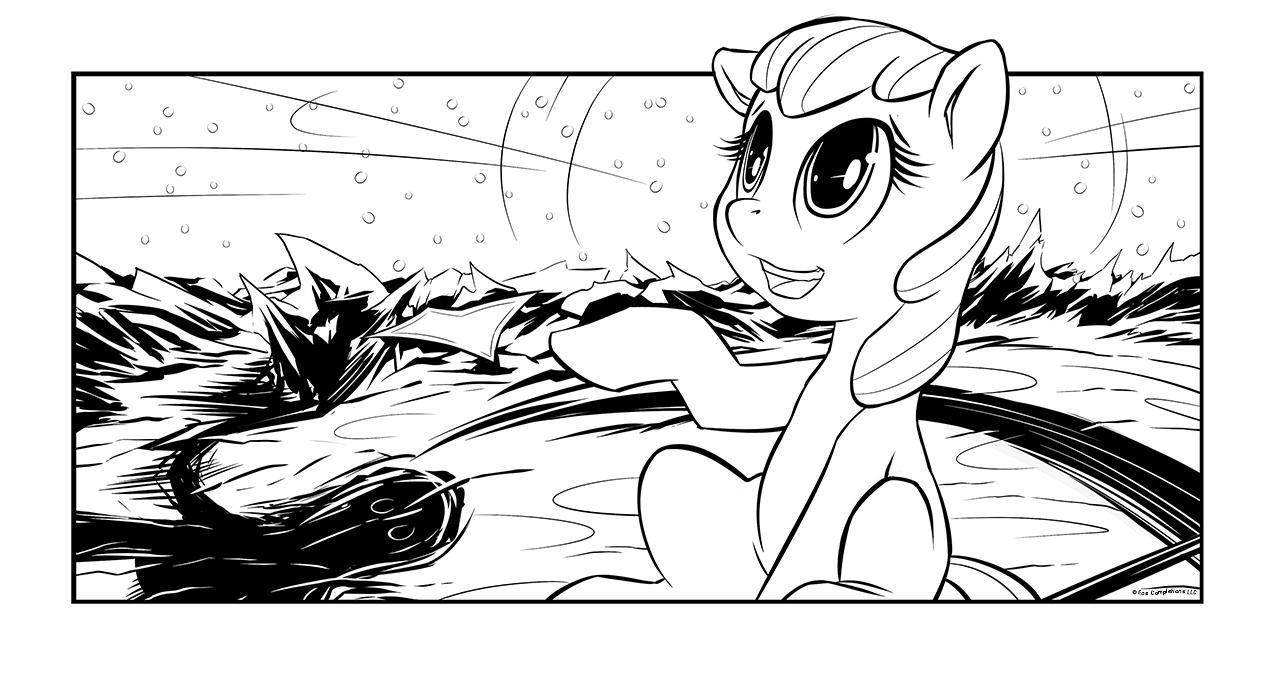
\includegraphics[width=0.9\linewidth]{image20.png}

\begin{intro}
And when the party's over we'll gather `round for a group hug!
\end{intro}

\englishdaytimeplace{14}{12:35 A.M.}{Emerald Shores, Big 52 S Branch}

Against the din of waves crashing into the rocky shore, Puppysmiles sat facing a gravestone. Her group of friends argued a short distance away, but she could only hear the Voice whispering inside her head. It spoke of pacts and promised dreams.

``Yes, yes, just\dots make all of this stop.''

Henrietta barely heard Puppy talking behind her, but she felt a sudden chill in the air, like a cold night's breeze, bringing with it the creepy sensation that she had just woken up from a bad dream but couldn't remember what it was about. Suddenly, what Puppy had said seemed a lot more important.

Everypony turned toward Puppysmiles. Was she talking with herself? Make what stop? How?

As Henri approached, she could see that Puppy's eyes were closed and her head hung low. Her mane was rapidly changing color, turning dark blue from its original blonde. ``Puppy? Are you okay? What\dots I\dots I think that you have something in your mane.''

When Puppy spoke, it was with a different voice. Like the sound made by a chorus of ponies calling from the bottom of a cave. ``I salute you, my humble minions. I'm finally here among you, bow at the dawn of a new era!''

Henri cocked her head and raised both her eyebrows. ``The what of a new what? Puppy, what's going on?''

Sidekick's eyes turned from red to blue, and it took up position on Puppy's flank, standing like a sentry. The creepy new Puppy continued. ``I am not Puppysmiles. I am Creepy Voice, a child of the Stars, and your new ruler. Under my guidance, a new Equestria will rise.''

Scold shook his head and looked over at Molten Gold. ``The Stars? Like in ancient zebra folklore? Those Stars?''

Scold's question was interrupted by Henrietta's laughter. ``Creepy Voice? What kind of name for a villain is that? I mean, really? Creepy Voice? Did you come up with that all by yourself?''

Puppy stepped back, with an embarrassed expression that rapidly shifted to anger. ``It\dots it is a name you'll learn to respect, fools! Now bow to me and return to your towns, announcing my advent!''

Trigger Happy snorted, stepping in front of the other ponies. ``Or else?''

The blue flames that burned in Creepy's eyes expanded until they completely filled her helmet. A blazing cobalt crown appeared above her head, and more blue fire sprouted from her back, forming a pair of ghostly wings. ``Or else, I will devour your souls!''

Happy hesitated, looking at her while Lonesome Pony muttered to Scold. ``Can she do that? Can she eat souls?''

Scold looked back at Lonesome and shrugged. ``How am I supposed to know that? If she really is connected with zebra dark magic, then it's possible. Only I don't think she's strong enough for that just yet.''

He raised an eyebrow. ``She isn't?''

``No, she's still manifesting, just look at how that fire of hers is flickering. I think I know how to stop this story before it even begins.'' Scold spoke in a very low voice while Happy kept the creature occupied. Molten Gold and Lonesome Pony listened to him with all their attention.

``I think that I can sever the bond that ties this entity and Puppy's soul together. Without a soul to feed on, Creepy Voice, uh, that creature, won't be able to manifest itself and will be banished.''

``So, what are you waiting for, an invitation?'' Molten asked impatiently.

``No, I'm not strong enough to do this on my own. It's a ritual, but it's long and complicated, and meant for unicorns only. No offense, Gold.''

Molten shrugged. ``No offense taken. So basically you're telling us that we are going to be fucked by a zebra demon with a foalish name?''

``Hey, what's going on? Does the egghead here have a plan?'' White popped his head into the trio of ponies, interrupting the conversation.

``Actually, yes, but I need some minutes to figure out the details, help Happy keep Creepy Voi---no, really, what kind of name is that?'' He facehoofed. ``Well, keep her talking while we try to pull this off, okay?''

White nodded and turned on his tail, trotting toward the trio composed of Henrietta, Trigger Happy and Jammed Gun. ``Hey, Your Highness, did you mention something about a new era? Can you elaborate on that part? Will it be better than the manure we are swimming in at the moment?''

The nightmare stopped considering Henri and her annoying question about names and turned toward the new arrival. ``Indeed! My magic is far superior to that of mere ponies, with it I can heal this poisoned land and bring about a new reign of prosperity! Your violent lifestyles will be at an end. I won't allow my subjects to squabble amongst themselves. Instead you will build immense temples in my honor! All you have to do is worship me, and pay tribute to me and all the problems in your life will be solved!''

White nodded at the response and tilted his head. ``Well, that sounds mighty interesting, but may I ask what you mean by paying tribute to you?''

She smiled before sitting down and closing her eyes, acquiring an air of mentorship. ``Absolutely. Your master, that is me, will ask very little for the good of many. Aside from your worship, I require a pony sacrifice every full moon from each major city. In return, I will cleanse the land poisoned by ponykind, allowing you to grow food and live your lives under my rule!''

Trigger Happy cocked her head, frowning. ``W-what are you going to do with sacrifices?''

Creepy Voice waved her hoof, dismissively. ``Never you mind.''

Henri and Happy had their mouths open, listening at what she was saying. Happy drew her weapon, but she stopped when she noticed White's gesture to wait.

Henri, on her side, scratched her head. ``Yes, but\dots will you give us back Puppy?''

The nightmare blinked her eyes for a moment, surprised. ``What? She doesn't want to come back. She is sleeping and dreaming, in a place where nopony can hurt her. We made a pact.''

At that reply, Trigger Happy snapped. ``You did a what? Listen, I know my friend Puppysmiles and how easy she is to trick! Whatever pact you made, it's not valid! You can't just\dots just talk a foal into something and pretend it's legitimate! Let her go!''

The nightmare laughed, with a silvery tinkling voice. ``Tee-hee, you're funny! Why should I yield a perfect soul to possess? Her obsession trapped her on this plane and as long as she sleeps, she will never realize the truth. So no, I'm not letting the foal out of her dream, but on the other hoof, I'm offering all of you the privilege of being my heralds so you can announce my coming to all of Equestria.''

``So, long story short\dots'' Henri tilted her head. ``You're Nightmare Moon?''

``Well, no\dots I mean, yes\dots I mean\dots Nightmare Moon was more ancient and powerful than me\dots'' For a moment the creature hesitated, but she seemed to recover almost immediately. ''But I am more than strong enough to shut your stupid beak!''

Henrietta deadpanned. ``So basically\dots you're a newbie. A Nightmare Noob.''

Trigger Happy burst into laughter, rolling on the grass as she fought for breath. Mister White facehoofed, while the other three ponies stopped talking for a moment, trying to understand what was going on.

``ENOUGH! THAT'S IT! THERE'S PLENTY OF SUBJECTS I CAN USE, I DON'T NEED YOU, USELESS BUNCH OF\dots OF IGNORANT WEAKLINGS!''

Henrietta snickered. ``Said the filly that can't count beyond four\dots''

``YOU INSOLENT LITTLE\dots YOU WILL SUFFER!''

``No, she won't! Bad monster! Stay put!'' Scold stepped in front of Henrietta, staring straight into the Nightmare's eyes. ``We will banish you forever, with the power of science!''

``Tee-hee,'' The creature giggled, evidently quite capable of shifting from anger to mirth on a whim, and dismissed the scribe with a wave of a hoof. ``Don't make me laugh! Science! Do you have the slightest idea of what power you are facing? Oh for Nightmare Moon's sake, try something more believable!''

Scold smiled, not very impressed by the nightmare's reaction. ``Oh, so you want the details? Very well, then listen carefully. Since I already had the opportunity to check Puppy's suit, I did some research and I found some interesting clues. Your very existence in this place is caused by a foolish attempt at using necromancy as a life saving device, but I know how to fix that horrific mistake the Ministries made! The talisman itself has proved to be almost impervious, but the spell inside is more than unstable. The way your flames wax and wane make that abundantly clear. Now, I have some unicorns here and even if they don't know a thing about dispelling magic, I can tap into their power for as long as we need. So, guess who's getting dispelled today?''

``What the\dots'' The demon stepped back, with an expression of real concern on her muzzle now.

``All right everypony, I'm casting the spell, you just clear your minds and this nightmare will be over! Let the magic flow!''

A flash of light exploded from Scold's horn and shot between the assembled unicorns, each of them sending out ethereal threads that became woven into a mighty spell.

Happy closed her eyes and let the magic flow through her, quickly followed by Mr. White and Jammed. Soon all their horns were glowing a brilliant white and the light expanded until it had enveloped the whole hill and everypony on it.

Henrietta grit her beak tightly and was forced to shield her eyes from the blinding glare. Something that Scold had said didn't sit right with her. He was going to stop the demon by destroying the necromantic spell being used as a life saving device, but wasn't that what was keeping Puppy alive?

Henrietta turned toward the old scribe. ``Wait! Are you trying to kill Puppy?''

Scold didn't reply, but from within the shining cloud of light the monster's voice confirmed Henri's fears. ``Fools! If you break the spell, the foal will die with me!''

``No, fuck, NO! You're not going to kill her, you fucking unicorn!'' Roaring, Henri charged at Scold, slamming into him so hard he flew for a couple of meters before landing heavily on his back. He screamed in pain and lost focus on the spell.

The light exploded in a rainbow of colors, spreading all around and dancing in every direction, but without a pattern. It was more like a giant disco ball gone crazy and rolling along a corridor than a real rainbow, and when at last the light died\dots

Nightmare Noob opened an eye, uncertain of what was going to happen next. Everything seemed to be still and silent, so she dared to opened the other eye too, and looked at the confused ponies in front of her. An evil smile appeared on her now very satisfied muzzle.

``So, in the end, Puppy's griffon friend proved to be very useful to me. But next time you might want to pick better allies for yourself, yes?'' The nightmare chuckled. ``Oh, silly me, there won't be a next time, since now you're all going to die.''

Scold shook his head as he got to his hooves, still dazed by Henrietta's tackle. ``What\dots why did you stop the ritual, you featherbrain? It was working!''

The other unicorns looked around at each other in a stupor, struggling to stand after the exhaustion of casting. Molten Gold tried to wake Mister White, while Henri advanced on Scold, with a grim, accusing stare. ``You\dots you won't take Puppy from me! There must be another way, I'm sure of it!''

``But\dots you stupid deluded brat! The foal is already dead! We're trying to save the Big 52 here! Come down from your\dots your `wonderful dreaming place' and get real!'' Scold was practically foaming at the mouth. Henri had disrupted their best chance to win, and now a lot of ponies were going to die because of her.

The nightmare savored the taste of crushing victory that was still lingering in the air. ``Oh, this is so tempting\dots Looking at your little argument is a real treat, but I have a schedule.'' Creepy Voice looked at Sidekick and in that moment the ghoul's eyes turned night blue. Sidekick turned toward the ponies like a hound. Nightmare Noob smiled. ``Let the games begin. Go, my minion, teach that chicken some manners.''

Sidekick crouched, ready to pounce on Henri like a cat on a mouse. The griffon was so focused on her argument with Scold that she didn't notice the ghoul jumping until it was too late. She didn't even hear Trigger's warning.

The impact sent Henri and Sidekick rolled down the hill, a whirling ball of hooves and claws. Henri fought without thinking, her predator instincts being all that kept her from being crushed by the foal's unholy strength. She tore with her talons and punched with her fists, dodging the return strikes and knowing that a single hit would be the end for her. The melee continued, both figures locked in a dance to the death even as they tumbled over the edge and fell to the rocks below.

Creepy Voice watched as her minion vanished from sight and shrugged. ``Oh well, meanie chicken broke my toy. It seems that I'll have to do everything myself, as usual. So, who's first?''

Lonesome Pony and Molten Gold exchanged a quick glance before opening fire. They emptied their magazines at point blank range, the bullets tearing through the Nightmare like a hot knife through butter.

Dozens of holes dotted Puppy's chest but they didn't seem to have any effect at all. Many had already begun to close. ``It's hard to kill something that's already dead, isn't it?'' Creepy Voice giggled as she lifted Lonesome Pony with her magic and slammed him into the tree. The pegasus hit the trunk with a wet, crunching noise, and fell to the ground unmoving, his back bent in an unnatural way.

Not even checking to see if Lonesome was actually dead, the nightmare turned toward Jammed Gun. ``So, I reckon you're with the sweet mare there? How cute, you'll die together, like the protagonists of some cheap old play! Any last words?''

``Actually, yes.'' Mister White smiled a little as he interrupted Creepy Voice and levitated a radio from his saddlebags. ``Plan B.'' His eyes narrowed. ``We've got backup.'' With a sound like distant thunder, sniper fire blew apart Pup's helmet and ripped away one of her legs.

The wicked creature roared. Spreading her wings, she flew up into the sky and conjured lightning from the clouds. The bolt struck the ferris wheel like a hammer, heating the metal and weakening the last joints that still allowed it to stand. The gigantic metal structure creaked and screeched, before collapsing on the small building that Sage Brush and a couple of acolytes were sniping from.

``No! Sage!'' White turned toward the town, looking at the rubble that once had been his nephew's hiding spot. No, this was\dots this wasn't going as planned at all!

A salvo of missiles streaked through the air toward the creature when she was far enough from the ponies below, shrouding her completely within a flourish of explosions. The rangers charged from their hiding spots in town, discharging every weapon they had in the monster's direction.

The battle had begun.


\horizonline


Henri groaned. It was all dark, cold and wet. Her bones ached in places she didn't even know she had, and she was almost sure that something was completely wrong.

A sweet and merry voice hammered like a pink flash in her head. \emph{``Oh don't worry, it's just you being your usual meanie self\dots nothing else!''}

``A\dots meanie what? Am I dead?'' Her headache was getting worse, while the sound of explosions and ponies screaming thundered in her ears. There was a\dots a thingy, something like a pink dot, dancing in her head and speaking to her.

\emph{``Silly chicken, you're not dead, \emph{duh}! You're just a bit confused and somersaulting down six meters onto those rocks didn't help at all, but I'm sure you'll be okay lickety split! Dashie did that all the time and never got hurt!''}

``Puppy\dots how is she? I-I must save her!''

The pink dot moved a bit, shifting from a colloquial, merry attitude to a more accusing one. \emph{``Really? Because it seems to me that you're simply trying to hog her all for yourself!''}

``What the\dots what the fuck are you blabbering about? I just want her to be safe!''

\emph{``So that she can stay with you forever and ever?''} The voice started fading. \emph{``Whom are you wishing well? Poor little Puppy or poor lonely Henri?''}

``I\dots I don't know anymore. But I\dots I want to make her happy. She seems so different, like a distant memory that doesn't want to fade. I don't want to lose her, but she seems to be unable to think of anything else but her mother, like a\dots a recurring nightmare!''

\emph{``Or maybe a sweet dream that doesn't know how to fade. Maybe she just needs a last, little help from her very best friend.''} The voice had gradually changed. At first it had sounded like an overenthusiastic youth, but now it sounded like an old mare. Somehow it was very, very familiar to Henri, reminding her of the dreams she had had when she was prisoner in Sun City. \emph{``There's just one last step to trot. Find Puppy's rock and fulfill its destiny.''}

With a gasp, Henri opened her eyes, finding herself in the middle of a rocky beach. She was lying on what was left of a badly crushed Space Ensign Sidekick. The ghoul had taken the brunt of the fall and was now just a flat squashed yellow bug. Henri drew one of her .45s and made sure that the creature was completely gone, putting another two holes in its head before checking the surroundings.

Up above her head, a pony flew over the ridge, screaming as she was sent out to sea. The dark magic faded, and she kept going for a good two hundred meters before splashing in the cold waters.

Henri tried to ignore the sounds of battle coming from above her head and gulped down a healing potion as she began her search for that stupid stone. ``Puppy's stone, Puppy's stone, how the fuck am I supposed to find a damn stone in the middle of a rocky beach? Magic Rock my ass!'' She scowled at a nearby rock and kicked it hard, sending it flying into a rusted metal box a few meters away. The rock rebounded and, of course, hit Henri squarely between her eyes.

``Fuck!'' She rubbed her forehead and picked up the offending stone from the ground. Every rock had its voice, and Henri knew this one very well . ``That's the last time you get one over on me. So what now? You hit a metal box, dumb rock, were you trying to tell me something? What are you, some sort of rock of destiny?'' Henri snickered as she approached the box, and introduced its padlock to \emph{The Rock Of Destiny}.

``At least\dots''

\emph{CLANK!}

``You're being\dots''

\emph{CLANK!}

``Useful!''

\emph{CRACK!}

``Very well, let's see what's inside the treasure chest.''

Some papers, an old brushable Applejack doll, some photos\dots Henri took the pictures and looked at them. In one there was Puppysmiles, only younger and without her radsuit. She was smiling in front of a carrot cake with four candles on it. There were some other ponies in the background. It seemed to be a birthday party. On the second picture there were a white stallion and a purple mare, and they were sitting in front of an old wooden sign announcing that they were entering the town of Appleoosa. Between the two ponies sat a pouting Puppysmiles, as if she didn't want to take the photo or be in that place at all. She seemed even younger in this picture, maybe three. Henri turned the picture and found a note: \emph{Last trip with Better}. A third photo showed Puppy dressed in a smock, and sporting a big blue bow in her mane. She was smiling, proud of her new dress. Another note, written on the front this time, said: \emph{Puppy's first day of kindergarten}.

Turning the last photo, the young mercenary found some weathered lines written on the back.

\medskip

\emph{In a different place and in a different time, beyond the horizon, we will be together again with Dad, and I'm sure I'll be proud of you.}

\emph{Because Mom will always be proud of her little sunshine.}

\emph{I love you.}

\begin{flushright}
\textbf{Mom.}
\end{flushright}

\medskip

A missile flew over the ridge and exploded on the shore, illuminating just for a moment the tears running down Henri's face.

Henri sighed, finally giving in to the truth in front of her eyes. ``She\dots she never belonged here\dots Fuck.'' Henrietta rubbed her eyes, putting down the photos. ``Fuck, why does it have to end like this? WHY?''

A new explosion painted the sky red. Ponies up there were dying, fighting something that was already dead. Dying because she wanted to keep Puppy for herself instead of letting her go, as it should have been. Now Henri knew what had to be done. Still, that didn't mean she had to like it. ``Not fair. Not fair at all\dots''


\horizonline


Paladin Gauss's eyes widened as the missile he'd just fired was thrown back at him.

``Gauss! NO!'' Cold Shower could only watch in horror as the explosion took away one of her oldest friends. She turned toward the Nightmare, her eyes full of anger and pain. ``Stupid bitch, why won't you die?'' The barrels of both the miniguns mounted on her power armor span up and she fired until her guns were empty, but the bullets bounced harmlessly off the nightmare's shield and were completely ignored as the creature launched a second acolyte into the ocean.

Creepy Voice had already killed two rangers and thrown several other attackers onto the sea, but with all these ponies around she was getting confused. How was she supposed to fight all of them at once? Really, these stupid equines didn't even know the rules of a proper duel! She was growing bored of their little game. Yes, killing ponies could be fun, but it seemed pointless, especially when she had more important things to do, like take over the world.

Who was supposed to be the leader of this bunch of idiots? Oh right, the old scribe\dots Creepy Voice smiled with evil on her mind. ``So, where is that guy with the cape?'' Landing in front of the old pony, Creepy Voice folded her ethereal wings and faced her adversary, not even trying to hide her amusement. ``Here you are! Scold, right?'' There was a pause, while he looked confused at her new change of mood, but the nightmare cut it short. ''Very well, die.'' With her magic, the monster grabbed his heart and squeezed. Scold collapsed with barely a whimper.

In the same moment, Henrietta flew over the ridge, landing again on the tomb's hill. The scene in front of her eyes made her cringe. This was her fault. All of this was happening because of her selfishness. Ponies fighting, ponies dying, this wasn't what Puppy would have wanted at all. It was time to end it. ``Puppy! Puppy, listen!''

The nightmare let out an annoyed sigh and turned toward Henri. ``Hey, it's not your turn yet! Don't you know that there's a list? I'm almost finished with this one, then I'll be killing you too, so don't push and keep your ticket ready!''

Trigger Happy crawled toward Scold while the nightmare was busy giggling at her own humor. Happy tried desperately and uselessly to revive the scribe. Their numbers were being mowed like a wheat field in front of a reaper. Molten Gold was struggling to break free from the tree he had been impaled on, Lonesome Pony had already passed out with his back broken and even the well equipped and combat trained rangers were losing ground. This was the end. They were all going to die here. For a moment, Trigger felt sad, she really, really wanted a foal of her own to love and care for. 

``Puppy, wake up! You\dots You can see you mother for real!'' Henrietta kept screaming with her high pitched bird voice. She was actually quite annoying. ``This Nightmare is a bug and a stinker! You're cooler than that! You learned from the best!''

Creepypup snorted. ``Aren't you even able to wait your turn to die?'' A halo of dark magic surrounded a large chunk of road and hurled it toward Henri, but she was agile and dodged it easily. ``Now I am disappointed, bad chicken! Do not make me come down there!''

Henrietta flew in front of Puppysmiles and pressed her beak against Puppy's glass helmet. ``Puppy, you moron, you are dead! D.E.A.D.! Just like your mom! Are you so stupid that you don't even realize how to die? Dump this idiot and go with your parents! Please!''

``What?'' The nightmare blinked her eyes, startled by Henri's sudden assault. What was she saying? Was she trying to speak to Puppy? Oh no, no no nononono! ``Shut up! She can't hear you, fool!''

``C'mon Puppy, wake up! You're not forced to stay here! I\dots I don't want you to stay here with me, you have to go! I'll be fine! Just\dots''

Henrietta was trapped in a blue corona and her body started to twist, producing disturbing snapping sounds. Creepy Voice looked straight into Henri's eyes, with a stare full of anger and hate. ``You. Die. Now.''

Henrietta smiled weakly, unable to resist the powerful magic crushing her body. ``Puppy\dots Mom is\dots just over the horizon.''


\horizonline


Puppysmiles sat in front of a pond, looking at the fishes that swam within. Everything around her was still and calm. A blanket of snow covered the ground and the clear sky showed hundreds of stars. She wasn't happy, but somehow she wasn't sad either. It was like being dazed, everything seemed so muffled and unimportant. It was just her, the snow and the fishes in the pond.

Puppy wasn't aware of how much time passed since she sat there, but it wasn't so important. She just wanted to forget\dots she couldn't remember. Well, maybe it was actually working. At least, until a weird goldfish poked its head out of the water.

``Puppy, you moron, you're dead!''

``Wut?'' She tilted her head, then checked her hooves and her tail. ``I'm not dead, stoopid fish!''

A second fish poked it's head from the pond, this one spoke in a feminine voice. ``C'mon Puppy, wake up! You're not forced to stay here!''

``Henri? Why are you a fish now?'' Puppy giggled. ``Silly Henri, fishes don't talk!''

Frost began to creep over the pond, but a third goldfish jumped out from the water, talking again with Henri's voice. ``Mom is just over the horizon!''

\rcpr{``Mom, where did Dad go?''}

\rcpr{``He's somewhere beyond that rainbow, Puppy.''}

\rcpr{``Will\dots will he come back?''}

\rcpr{Mom didn't reply, but Puppy really, really wanted to see Dad again.}

\rcpr{``Can\dots Can we go where he is?''}

\rcpr{``Yes Puppy. One day, maybe not tomorrow, or not the day after\dots In a different place, and in a different time, we will be all together again, okay? Just\dots just over the horizon.''}

\rcpr{``Pinkie swear?''}

\rcpr{``Cross my heart, hope to fly\dots''}

``Stick a cupcake in my eye\dots'' Puppy looked up in the sky. And finally saw him.

``---really, really late and I know I actually have all the time in the universe, but I hate these kinds of anomalies, and this one has been going on for two hundred years! I'm beginning to lose my cool, because there are a lot of better places I'd like to be rather than here!'' A skeleton wearing a black hood was talking in Puppy's direction, but he seemed to talk to himself more than her.

She smiled. That skelly pony was funny, he was talking like those grumpy ponies at the veteran retirement house! ``Hi, I'm Puppysmiles! Have you seen my mom?''

``Oh, please! Not that litany again! I'm going to resign, or strike! Or strike and then resign!''

The skeleton pony was interrupted by the giggling Puppy. ``Tee-hee, skelly pony is funny!''

Stopping his monologue, the grim reaper finally noticed that she was looking at him. ``You\dots can you see me? Is this some sort of prank? Because if this is a prank, I'm going to give up for real this time.''

Puppy tilted her head. ``A prank? I hope not! Last time I made a prank I was spanked ultra hard!''

The pony paused for a long moment before falling down on his haunches with a ghostly sigh. ``At last\dots''

Puppy trotted near to the weird looking stallion and sniffed his clothes. ``Ah, who are you, pretty skelly pony?''

``Me? I'm the Grim Reaper, Death, the Inevitable End, the Black Stallion\dots'' From Puppy's blank stare, the skeleton realized that he was just wasting good words. ''But my colleagues call me Mort. Long story short, I'm the guy that shows the deceased how to reach their afterlife.''

Puppy tilted her head, confused. ``So\dots Have you seen my mom or not?''

The skeleton shook his head. ``You're a lost cause.'' A silvery ticket covered in shining pink letters appeared in front of Mort and gently fell like an autumn leaf between Puppy's hooves. ``Here, take this ticket. It's worth a ride to the other side. Remember, not everypony gets the silver ticket. It's a really special one that will bring you there lickety split, so be grateful.''

Puppy's eyes grew bigger. ``I\dots I am going to see Mom? For real? No more pink arrows, or stoopid bullybots, or falling houses? Just\dots Mom?''

Death nodded. ``Exactly.'' Mort paused for a moment before continuing. ``It must have been hard. This is my personal way to say I'm sorry for not being able to help you earlier.''

Puppy stopped listening as soon as the pretty skelly pony had said what she wanted to hear. ``Yush!'' Puppy hugged Death for a moment, before looking at the pond which had now completely frozen over.

``Oh right! Henri! Just let me say bye to my friends!'' Puppy turned on herself and the whole scene with the pond and the snow exploded into a thousand shards, dissipating into nothingness and revealing the battlefield around the graveyard.


\horizonline


``\dots Just over the horizon.'' Henri's eyes grew clouded as she slipped into unconsciousness.

As soon as Henri had said those last words, the Nightmare's eyes flared pink and for a moment her expression changed completely. ``Bye bye Henri! A pretty skelly pony is sending me where Mom is, and this time with a super shiny ticket!''

The pink in Puppy's eyes faded away one last time and all the lights on her HUD turned red, signaling an endless sequence of system errors.

{\mt ``Warning. Subject 001 Puppysmiles cannot be located. Warning. Power level is critically low. Warning. Self repair function not responding. Warning. Hardware not found. Warning. General shut down in five, four, three, thank you for using Ministry of Peace technology. Have a nice day, and please, be safe.''}

With these words, the whole HUD on the helmet disappeared, leaving only the shocked face of Creepy Pup staring at the now empty glass.

The monster stepped back in horror, releasing her magical grasp on Henri, who fell to the ground and rolled a few meters downhill. ``What have you done, fool? I'll kill you all immediately, puny insects!'' The monster stretched her wings, ready to release a new wave of magic, but something was wrong with her. The suit had begun to deflate like an old, empty leather ball. ``What\dots what's going on? I'm melting! NO, NOOOO!'' Small eruptions of pink gas leaked from every hole in the fabric, while the monster fought to keep her grasp over what was now an empty husk.

``You! You have not won! I will be back! Ponies make the same mistakes all the time! I'll be baaAAH---'' Creepy Voice's face melted in a pink eruption, filling the helmet with a curtain of gas. For a moment the suit inflated like a party balloon as whatever force that kept the pink ooze in a fluid form stopped working and the pink agent reverted to its usual gaseous state. As the scream from the Nightmare reached its highest note, the suit's locks failed and the gas exploded out of the harness, making a sound like a whistle.

The ponies that still were capable of walking grabbed the wounded and dragged them away, far from the expanding cloud of pink death that had started to lazily invade the whole hill.

``Go go go! Let's get away from that stuff!'' Cold Shower dragged away what was left of Gauss, following the others.

Creepy Voice continued to scream as they fled, a long wail of anger and agony.

Half dragged and half pushed, for a moment Henri regained a spark of lucidity. Everything seemed distant, and she felt as if she was floating in a warm place, lulled by gentle invisible waves. And in the middle of that moment of peace, she heard Puppy's voice. ``Hey, hey Henri\dots''

Henri groaned. That foal wouldn't know the difference between a wrong moment and the worst possible moment even if she bumped into it with her muzzle.

Puppy ignored Henri's mental complaints. ``Listen, I has really no time, but I wanted really really REALLY to say I'm sorry, but I has to go\dots I\dots we are still friends, right?''

Still friends? That was a weird question. Puppy was more than a friend, she was something more, something bigger, in Henri's life\dots

``Really? You\dots you liked me that much? I know! We can be sisters! Yush! Henrietta Days! I lovelovelove it!''

Henri chuckled, still half dazed by the Nightmare's embrace. Henrietta Days\dots Sure. That was totally going to happen\dots Adopted by a pony.

``Okay sis, gotta go I love you bai!'' And with those last words Puppy's voice faded away as the griffon passed out again.


\horizonline

\englishdaytimeplace{14}{17:00 P.M.}{Emerald Shores, Big 52 S Branch}

\rtpr{Good day, Big 52! And for once I mean it! This is DJ Good Stuff and you are listening to Radio 52, the radio of good news!}

Boisterous triumphant music played for a few seconds.

\rtpr{I've been receiving transmissions from Ironworks and Broccoli since this morning and now I can safely say that the news is confirmed: the Wild Herd was defeated! WOOHOO! Yes my little ponies, you heard me well, the good guys trotted down to Ironworks and kicked some raider ass for good!}

The DJ laughed enthusiastically, evidently too happy to keep even a shade of professionalism.

\rtpr{I still lack the details, but it seems that the Applejack's Rangers along with a group of volunteers, and please note that Lonesome is among them, assaulted their camp very early in the morning and caught them by surprise, killing a large number of raiders and routing the others. This is how things get done `round here, raiders! You better think twice before you mess with us!}

Good Stuff paused for a moment before continuing; in the background there was a sound of shuffling papers.

\rtpr{Okie dokie, now, for those that have friends and relatives in Ironworks\dots The situation seems dire. Most of the adult ponies have been killed during the siege, but there are still some survivors, mostly the elders and the foals, with a small group of guards that found shelter inside Ironworks's Stable. I don't have a list of the survivors so far, but I'm working to get one, so expect some more news during the day.}

\rtpr{In the other news, Splendid Valley was hit by a huge explosion that completely devastated it. Apparently, this has something to do with the Enclave, since---}

Trigger Happy turned off the radio and turned toward the Hill. The pink cloud had been scattered by the wind, but not before coloring the solitary tree in sugary pink. Right under the tree stood two graves.

Henri looked at the last stone in her claws: \emph{The Rock Of Destiny.} She sighed, weighing Puppy's weapon before putting it on top of the small mound erected next to Rainy Days's grave. A small toy pony sitting on a foal-sized red scooter had been left in front of the memorial, almost like a bunch of flowers.

She opened her beak, looking for some words to say, but closed it again without thinking of anything. Mister White arrived from town, carrying a rusted road sign. The stallion patted Henri on the shoulder before taking a brush and painting two words on the metal plate. 

\begin{center}
	\textbf{---Puppysmiles Days---}
\end{center}

Trigger Happy approached the new grave, frowning a bit. ``Is\dots is that all? Just a name? It seems so\dots cold.''

He shrugged. ``It's how we have always done things `round here. Graves are not for showing.'' White looked away from Trigger, staring at the other graves on the hill. Cold Shower and Scold still sat in front of the numerous ranger graves. Sage Brush's tomb was sitting alone, facing north, toward Salt Cube City. White shook his head and turned back to Happy. ``It wouldn't be fair. Her grave is not the only one that was dug today. Let's stick to our traditions.''

Trigger Happy nodded and sighed before she turned away and approached Scold. The old unicorn was looking at a holotag in his hooves, but when the mare approached him, he put the object away with a sad expression. Happy kept her voice as low as possible while talking to him. ``How are The DJ and the Ghoul doing?''

Scold shrugged. ``Gold will survive. He just needs some radiation. Lonesome Pony\dots well, we will try implanting him with an artificial spine, but we lack the correct instruments, and I don't know if he'll survive the operation. Your coltfriend should be with him right now, so maybe you should go and check yourself.''

She lowered her eyes. ``I-I'm sorry for your losses\dots I could have taken all the guards from Tunnel Town with me, not just me and Jamie\dots''

The old scribe smiled weakly. ``It's not your fault, we had no idea of what we were going to face here. Those that gave their lives fighting against that horror will be remembered as heroes. I know it won't bring them back, but maybe this will give at least some meaning to their deaths.''

As soon as Trigger Happy departed, Scold trotted next to Cold Shower and sat with her in front of Gauss's tombstone. She was crying in silence; the two ponies were more than comrades, and the loss had been a bad blow for her.

``He was a good friend\dots You know, even when he acted like an ass.'' Shower was having a really hard time, trying to hold back her sobs as she spoke.

Scold nodded, wrapping a hoof around the mare's neck. ``Yes, he really cared about ponies. He knew what was important\dots'' His stare wandered across the graves. Four. Two paladins and two acolytes. The Rangers probably owed Puppy more than that, but it felt hard to accept it. Still, he didn't want to blame the griffon for that, it simply didn't feel right. ``We lost many good ponies, today. Acolyte Sugar Flavor and Scribe Scroll were still so young. I'll have to inform their parents.''

Cold Shower sighed, tears now running down her muzzle. ``Scold, please\dots{} Tell me it was worth it. I lost so many friends\dots I lost the pony I loved. Tell me\dots tell me they didn't waste their lives.''

``We are just ponies, Shower. We do what we can to make this land a better place day by day. The records say that in the last generation, in the Big 52's settlements cutie marks involving traditional works like masonry, farming and arts are slightly growing. Maybe things are getting better, and maybe our foals will see a greener Equestria.'' Scold looked at Puppy's grave. ``And maybe, one day, there will once again be a place where foals like Puppy will be free to play and make friends. Who knows\dots''

Henrietta rubbed her eyes as she left Puppy's grave and trotted toward the beach, looking at the waves. Henri checked that nopony was looking at her, and when she was sure of being alone, she took Silky Tail out from a bag, hugging the doll and hiding her face in the pink plushie. 

``Don't worry, sis. Tomorrow will be a better day.''

\clearpage

~\vfill

\begin{engnote}
		Level up! (20) No wait. You're dead. Sorry kid, better luck next time.
	
		New Quest Perk unlocked: Filly Luck - Requirements: Level 8, Minimum Luck of 7. ``All right, we were just surrounded, okay? And the droids were all over the place, got it? And we got, like, five shots left, okay? Then all of a sudden, we hear a ruckus from downstairs, and the next thing we know is that half the robots were brutally demolished piece by piece by Celestia-knows-who! With a stone! Real story, man, honest!'' Occasionally, when facing robots or feral ghouls, you can find some groups of them already dead, brutally killed with a stone. Go Puppy!
\end{engnote}





\backmatter

% NOTE: putting head style command here is OK

\fancyheadmanuallyenglish{Afterword}

\chapter{Afterword}

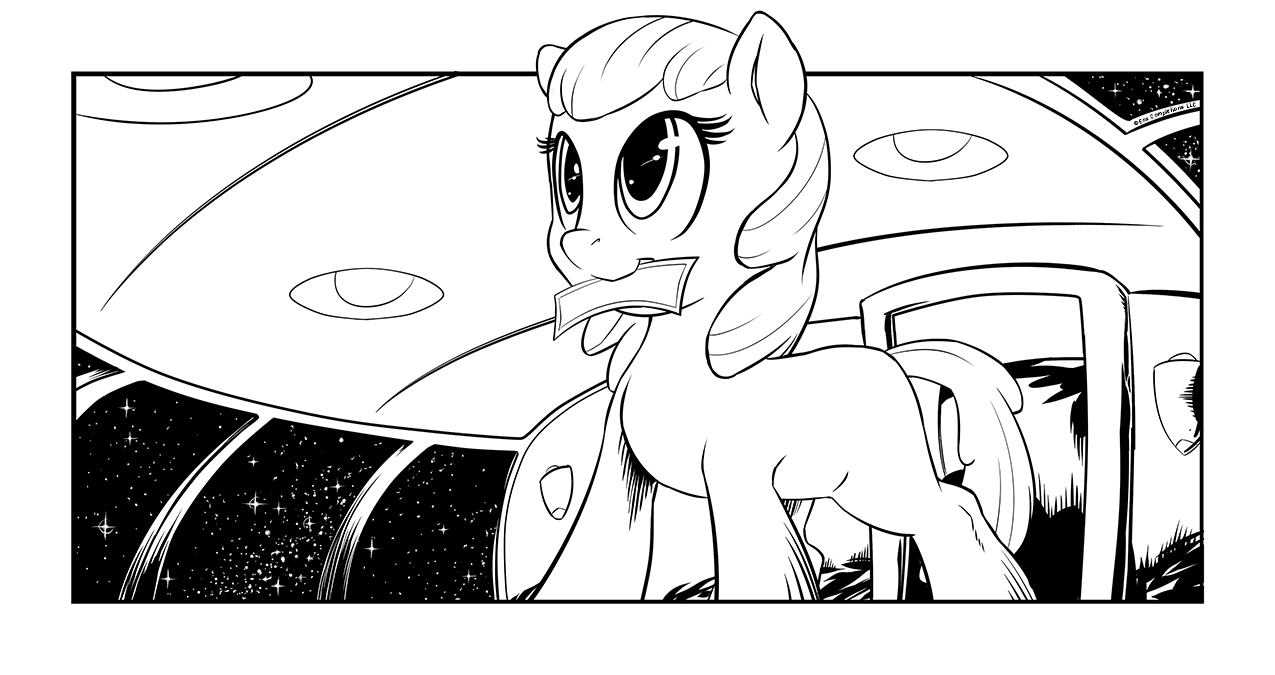
\includegraphics[width=\linewidth]{image21.png}

\begin{intro}
    Beyond the horizon, we will be together again.
\end{intro}

{\rt

``Oh, c'mon, you can't st- FZZT -rking right now!'' BAM BAM BAM! ``Hello hello? Test, test\dots onetwothree\dots''

``\dots''

``Okay, it seems to work. Very well\dots let's get started. First of all, my name is Watcher. My self imposed mission was to watch over the Wasteland, looking for lost ponies and groups of adventurers, hoping to eventually find those that carried the Elements of Harmony. Now, things are changing and I have friends that will help me with my task. I'm not alone anymore, and I finally have some time for doing things that I feel need to be done.

``And this is the reason why now I'm recording this tape and, just for this tale, I'm asking you to call me Mister Questioner. This is a story that could seem unimportant, or even silly, but it's about dreams, and memories. It's a story about two large, innocent pink eyes that couldn't see the horrors of our times and kept believing that somewhere, behind those ruined walls, inside the slave pens and even in the raiders' camps, everypony was still a pretty pony.

``And at the end of her journey, where the road met the ocean, the ghost foal that lost her mom finally found a place to rest. Sure, she was a little late, but I was told that when she finally accepted her fate, Puppy left with a smile.

``Like she were following an old postcard the filly went down the Big 52, showing everyone she met what ponies had been in the past and what they could still be. Somehow changing the way they saw themselves, making them see a better past, and making them wish for a better tomorrow. She wasn't actually trying to change the world, or even to save lives, but that might have been why so many ponies took notice. Since she was no preacher but simply herself, it was easy to see that there was no fanaticism or weird ideals in her; just a little pony with large pink eyes that knew, for a fact, that no one could really be that evil.

``And this\dots this is what happened in the few months between Puppy's arrival at Emerald Shores and today.

``The ponies of Emerald Shores came back to the town shortly after the Wild Herd's defeat: when they arrived from the NCA, they found the graves on the hill and the remains of the crushed ferris wheel; alas, what really startled them was that somepony had changed the name of the town on all the signs. Now the town is called Nightmare's Fall.

``The survivors of Ironworks started rebuilding the town, helped by their neighbours. Since the battle the settlement had a shortage of adult ponies, so the Rangers decided to settle in this town, making it their new headquarters. Not everypony was happy with this new situation, but the rangers proved themselves vital during the liberation of the town, and eventually even the most stubborn came to accept them.

``With Ivory Tower destroyed and Ironworks reduced at the shadow of its former self, Broccoli gathered all the ponies that didn't want to live in a ghost town or hadn't a home in which to live at all. The work in the fields improved greatly and the farmers diversified their crops, for the joy of the foals. Now they grow both broccoli and cabbage.

``The crater at Ivory Tower was filled by the seasonal rains and a small trading post has been built along the route between Broccoli and Rust Manor. The town is very small and lightly fortified, but it's growing fast and somepony is starting to build farms all around the lake. The town still doesn't have a name, but the traders call it The Hole.

``Rust Manor was attacked during the Enclave conflict; the town wasn't able to repel the attackers and the control tower was completely destroyed; numerous ponies were killed, but the survivors are already beginning to rebuild their home. It won't be easy, but nothing is easy in the wasteland.

``Sun City is still a war zone. The Sand Sweepers and a number of small bands are currently fighting each other to gain the control of the desert's gem. Since the Hired Hooves retreated from Sun City during the Enclave conflict and never came back, the settlement is still a dangerous place, avoided by almost every caravan. For those that dare to risk their lives, though, the inner town is full of old world technology that could make you rich for the rest of your life.

``Tunnel Town expanded on both sides of Sugartop Mountain and now it's the third largest town along the Big 52. The prices for using the tunnel have been cut considerably and the city began a service of long range patrols to keep at bay the groups of raiders and slavers along the Route in the town's territory.

``Salt Cube City is still the biggest city along the Big 52 and it has grown even more since the ghouls left the Dome. The Hired Hooves are expanding their influence even outside the Route, and have opened offices in the nearby towns. The Talons don't seem very happy with this policy, and tension between the two mercenary groups is rapidly growing.

``The Redtrotters didn't change very much: they stayed faithful to their tribal customs and are still charging the caravans that travel along their territory, but now foals don't have to pay the fee. This is not a big improvement, but the tribe has opened relations with the other settlements and they are actually trying to improve the safety of their part of the Route.

``The Applejack Rangers helped in reconstructing Ironworks, establishing their new base in the town's Stable. During the last battle at the Cave, all four of Ironworks' surviving paladins were dispatched to help with defending the place, and I had the opportunity to meet both Cold Shower and Scold. The battle was hard and Shower didn't survive it; she is now sleeping besides Gauss at Emerald Shores. Scold has grown distant after losing her; it seems that the old scribe is doomed to survive all his friends\dots a fate that I can easily understand.

``Happy and Jamie married and I was told that she is expecting. Since the marriage is quite a recent news, I think that they didn't expect to be celebrating again so soon. When asked what name they are planning to give the foal, Happy stated that she's still uncertain, but it won't be Puppysmiles.

``Molten Gold didn't stop his graverobbing career for long after the battle with the Nightmare. The ghoul left as soon as he recovered and sailed south on a steamboat, along with a group of adventurers. I haven't heard anything from him since then.

``SolOS and Pinkie 7 were actually able to become friends in the end. I was contacted by P7 a little after the first Enclave attacks; she was curious about this 'Questioner' Puppy was always talking about, so we had a chat and even if I don't think I'm going to trust her or SolOS any time soon, I think that they aren't going to give us troubles for a while. She actually scared me a bit when she told me about her and SolOS' idea of programming a new AI and naming it Puppy.SML\dots I hope that this was just a joke.

``Lonesome Pony recovered from his wounds and went back to Radio 52, keeping the Big 52 together with his encouraging speeches and all of his music. DJ Good Stuff is still working with him but when I tried asking when they were going to marry, both of them laughed at me. During the Enclave conflict Radio 52 kept broadcasting; it was small enough that the pegasi didn't bother to shut it down. The radio helped with organizing the defenses and boosted the morale of the defenders; it wasn't very much, but it was enough for those that fought during the conflict.

``Mister White trotted back to Salt Cube City; the loss of Sage Brush changed him deep inside, even if his sister never blamed him for it. After resigning his place of leadership, he became a traveling merchant and as far as I know, he's still running along the Route, bartering every sort of merchandise. This is just a rumor, but it seems that one of his guards is a unicorn mare with a tower as a cutie mark. Maybe he didn't want to lose the opportunity to hire somepony that had the guts to spank a Nightmare, or he simply wanted to give a raider a second chance\dots After all you gotta care, right?

``After Long Ears' demise, a new filly in her tribe got the Far Seer cutie mark, becoming the next shaman. I have no idea how their power works, but it seems to be some mix of powerful drugs and innate precognition; I just know that it is very tolling and quickly consumes the mare's body, so that a single pony sacrifices her life to help the tribe. A boon that brings a curse\dots

``There's still a pony that I never met in person, and I'm starting to doubt his actual existence. Puppy described him to me as\dots the baddest evil villain ever. Count Horse Tile. I asked several travelers and caravan guards, but no one has been able to give me a single clue about this cruel noble pony\dots I guess his mystery will remain unsolved.

``Henrietta is still running from the Talons. It seems that there has never been good blood between them and the Firebrights, and the young griffon is keeping up the family tradition. I tried to talk with Gawdyna, to see if some sort of truce can be arranged. I hope that Henry will accept to parley; after all she was Puppy's best friend, and seeing the girl die because of a feud that she didn't even start is something i rally don't want to see.

``The Wild Herd was dispersed and fled to their outposts on the coast again. This time they suffered heavy losses, both in numbers and in pride, but everyone knows that they will come back one day. Hopefully, even if they once more strike the Big 52, it will be without the help of an army of robots, and that could be enough to let the good ponies sleep quietly, for the moment.

``The Lost Herd seems to be gone. With Sidekick's death, the last of those damned souls found peace at last, and finally Equestria will be able to forget one of the many horrors of the war. May those poor foals find a deserved rest in whatever awaits us past this life.

``So, this is the end of Puppy's story. Did she really change something along her path? Will her action matter in the long run? I have--- sorry, I \emph{has} no idea, but I think I'll miss the way she talked, and the way she took everything so lightly. Another shard of the Equestria I loved is forever gone\dots but I still hope that I will live long enough to be able to see a filly like her again; but this time it won't be a ghost from the past, but a daughter of the present.

``And speaking of ghosts, the legend of the Ghost of the Big 52 is still alive, even if it seems more a Nightmare Night's tale than a real story. It's said that when the sun goes down and the moon is waning, a ghostly figure rides along the Route, silent like a shadow and swift like the wind. It looks for the souls of the wicked: slavers, raiders and the evildoers that lurk in darkness, waiting for easy prey. At least two groups of raiders were actually found dead along the route: they didn't show a single wound, their weapons were still fully loaded and they were clearly ready to strike\dots but they died on the spot, with no explanation. Killed by a presence that didn't leave a single clue. So, now I want to ask you one thing.

``Do you believe in ghosts?''

}

\horizonline

\englishdaytimeplace{4}{7:30 P.M.}{Downtown, Salt Cube City}

Sand Box turned the wheel left trying to make the airship fly against the wind, but it was an impossible task. Friend Force One was losing pieces along the way since the take off, and two engines had already failed. The ghoul slammed his hoof down on the intercom and yelled: ``Soft Air, we need more power! We're getting pushed back by a damn nightly breeze! I don't know how, but give me more knots!''

The reply from the communication device had more in common with an electrocution than an actual conversation, but it was about the balloon losing gas and the engines catching fire.

Sand box cursed, before talking again in the instrument. ``Okay don't worry, I've got a backup plan: we will crash the airship here, so that the wind won't send us back to Salt Cube city!''

If the reply from the other side of the line was a complaint, it never reached Sand Box. In that very same moment the whole world decided to become pure light.

Just an endless, blinding, perfectly silent light that enveloped everything. There was no pain, and there was no fear. Just light.

\horizonline

\englishunknowndaytimeplace

When Sand Box opened his eyes again he had the unsettling feeling that there was absolutely nothing wrong. Nothing at all. He took his time to look for a moment around the flying deck, trying to understand what happened. Well, the wheel was still there, the sky was all starry, the commands were working, the lights were all lit\dots

``Wait a moment\dots the lights are all lit? There are stars outside? What the\dots''

Yes, the airship was working perfectly, and by perfectly it meant that the whole damn room seemed as new as the day it went out from the docks. The floor was shining, the commands were clean, the wheel was even waxed! And the windows! They were so clear that you could even see yourself inside th---

And Sand Box saw Sand Box. Surprise on his muzzle was giving way to realization. Slowly, he touched his face with a hoof. It was\dots his real face, the one he had before becoming a ghoul! He was a pony again, he was\dots

Dead.

He was dead, this was the only possible reason for all of this. But if he was dead, why was he still on the ship? Was this some sort of afterlife punishment where he had to fly a ship forever, like the Flying Dutchmare? Were the others trapped forever on that thing with him? And why? He\dots he didn't want to fly forever, he had to see Agatha! She\dots she was waiting for him somewhere, he couldn't just\dots fly a stupid ship for the eternity!

FWEEEEET! A loud whistle interrupted Sand Box's shipwreck of desperation, making him turn towards the deck's entrance. A feminine voice announced her arrival while the door slammed open. ``Captain on the Bridge!''

A pink mare with a pink mane and big blue eyes appeared in front of the former ghoul; she was wearing a navy officer uniform and sported the largest smile Sand Box had ever seen on a pony\dots ``Miss\dots Minister Pie?''

Pinkie dismissed Sand Box with the wave of a hoof. ``Ah, call me Captain Pinkie, I don't like that ministry thing\dots it wasn't happy at all anyway.'' The young mare started jumping in every corner of the bridge, giggling and yelling enthusiastically. ``Yay! I knew that this little filly was going to fly sooner or later! Oh, oh, look! Look at this! All the arrows on the panels are pink exactly as I asked! It's\dots it's fantastic!''

The chief technician stood still with a confused expression on his muzzle, looking at the hyperactive pony touching everything while moving around at a speed that wasn't physically possible. ``I\dots can I help you somehow?''

Before Sand had the time to finish the question, he found himself staring into Pinkie's enormous blue eyes, nose to nose with her. ``Sure you can! They are all waiting for you in the lounge! Move that slow rump of yours and join the party! I'll get there as soon as I'm done having fun here!''

The stallion nodded, slowly stepping back towards the door and never losing eye contact with Pinkie Pie. She was a little bit scary, especially from the point of view of a pony that had just been dead for less than ten minutes. Once on the stairs, he turned on his tail and rushed to the airship's recreational bridge.

The saloon wasn't crowded, still it was quite populated, especially since Sand Box clearly recalled that aboard the Friend Force One there were just four ponies when it took off. Now instead he counted eight guests.

It was easy to recognize Soft Air from his typical military technician jumpsuit, and Peach Blossom with her blooming peach flower cutie mark was easy to spot; the middle aged mare with the stethoscope had to be Dr. Get Well\dots wow, she was quite a sight with all of her skin and muscles in their place\dots This left a griffon and four other ponies that Sand Box didn't recognize.

The griffon was sipping tea while reading a newspaper, sitting on a couch. He was wearing combat armor and had several weapons on him. Two of the ponies, a mare and a stallion, had the typical padded suit used under power armor and were standing side by side in front of a table with drinks and snacks. They didn't pay attention to the table anyway, being too occupied in nuzzling each other, seemingly at peace.

The third pony was sitting alone in front of a window, looking outside the ship. He sighed and shook his head, in his eyes was easy to read some sort of regret and resignation. As if he left too many things undone behind and wanted to go back. The fourth pony was a unicorn mare with a long cape; she had the Sand Sweepers traditional jewelry on her, maybe she was a dead far seer? The mare seemed different from the others, more a shadow than a real presence. She was also the one that trotted towards Sand Box when he stepped inside the room.

``Greetings, I see that Pinkie let you come down at last. I guess this means that we are ready to proceed\dots she should be here soon, unless she got lost again.''

Sand Box frowned. ``What is going on? Who is she? Who are you? Listen, I'm not a troublemaker but I'd---'' He stopped talking when the mare approached a door and pulled it open. A Pink foal with a blond mane and two big pink eyes trotted inside the room.

Puppy still had her pretty silver ticket in her teeth. She didn't understand how exactly she arrived in that place, but it didn't matter. There were games, and treats, and it totally seemed like a super fancy party! It was everything she always dreamed, and it was full of ponies to boot! And a Chicken!

Sand Box felt his heart sink in an icy grasp. Of all the ponies he was expecting to see, Puppysmiles was the last one. ``Oh, little one\dots I'm\dots I'm so sorry\dots'' How could this foal smile even in a moment like this? ``What happened? Who\dots how did you arrive here?''

Puppy tilted her head, unable to recognize the pony in front of her, but he seemed very nice, so it was all right. ``Hi mistur pretty pony! I am Puppysmiles, and I am going to find my mom! A super nice skelly pony gave me this super fancy ticket and sent me here! And I was told that Mom was just over there, after the ride!'' The little filly paused for a moment, checking the place. ``Ah, are we there yet?''

Sand Box blinked his eyes, trying to understand what the foal meant, but Long Ears came in his help, whispering in his ear, ``Her mother is dead\dots'' This only succeeded in making Sand's perplexity grow.

``You\dots you are happy to be dead?''

Puppy giggled. ``The nice skelly pony told me so, mistur pretty pony! But I feel fine and I'm going to find mom! This is, like, the best thing ever!''

``B-but\dots'' She was so\dots happy\dots and even if she was explained what was going on, what would have been the point of it? Sand Box smiled and nodded. ``Yes. Yes it is. Do you want to play something with the others until we arrive?''

In the meantime, the various ponies in the room had slowly gathered around Puppy. They were all looking at her with various degrees of perplexity or sadness. Cold Shower and Gauss approached the filly, the mare was the first to talk.

``I'm sorry that we had to fight you\dots I wish there was a better way\dots'' Gauss nodded for a moment, sighing deeply.

``Ah, why is everypony sad? Where are the pony games? I want to play hide and seek! Or pin the tail on the pony! And then I wanna dance, and\dots Oh, I hope the pony tail is pink! Pink is my super favorite color! I'm the bestest tail pinner ever!'' Puppy was already jumping on her hooves, trying to look beyond the small group of ponies.

Pinkie, now wearing a flight attendants uniform, followed Puppy through the door, and patted the foal on the head. ``I'm sorry Puppy, but there's no time for that! We've sailed through the Star Ocean, and now we have arrived! The ride ends here, fillies and gentlecolts! Thank you for choosing the afterlife airlines and have a pleasant stay!'' The pink mare moved rapidly towards the door, opening it and revealing to the other ponies a wonderful landscape made of green hills and small ponds.

Small herds of ponies dotted the meadows, while pegasi sat on the clouds populating a wonderful blue sky. The passengers trotted outside the ship, staring in amazement at the place. It seemed like a dream come true: here and there it was possible to see the roofs of some houses and on the distant hills there was a large apple orchard.

Even Puppy was left speechless in front of the beauty of the place; everything was perfect! The trees, the meadows, all the pretty ponies and the sunny sky! It\dots it was even better than Ponyville, it was so beautiful! The only thing that was missing was---

Puppysmiles froze for a second, her eyes staring into a small herd of ponies grazing on the borders of a daisy field. The smile on her face grew bigger and bigger as she galloped toward the ponies in the grass. One of the figures looked up and smiled at the incoming filly who was now crying with joy, unable to say anything but a single word.

``Mom!''





\chapter{Acknowledgements}

\begin{center}
    This fanfiction is based on \emph{Fallout: Equestria} by Kkat.    
\end{center}

\section*{Author}

\begin{center}
    Mimezinga
\end{center}

\section*{Cover by}

\begin{center}
    LimreiArt\footnote{\url{https://www.deviantart.com/limreiart/art/Pink-Eyes-513444372}}
\end{center}

\section*{Illustrations by}

\begin{center}
    Boiler3\footnote{\url{https://www.deviantart.com/boiler3/}}
\end{center}

\section*{Speical Thanks}

\begin{table}[H]
    \centering
    \begin{tabular}{ccc}
        Nyerguds & Damhoof & Easteu \\
        Aerondight & Arcane Scroll & Palacioskw \\
        Anonsamurai & & \\
    \end{tabular}
\end{table}

\section*{Typeset by}

\begin{center}
    RandomQuantum
\end{center}

\section*{Links}

\begin{itemize}
    \item Published on Fimfiction: \url{https://www.fimfiction.net/story/931/fallout-equestria-pink-eyes}
    \item English Ducument: \url{http://book.fallout-equestria.com/forum/viewtopic.php?f=3\&t=342}
    \item This Project on GitHub: \url{https://github.com/Ranqumn/FoE_pink_eyes_publish}
\end{itemize}


% ---------

\clearpage

~\vfill

\begin{center}

    \sout{Press any key to skip credits}
    
    (This function has not been provided yet)

    \vspace{\baselineskip}

    Thank you for playing \emph{Fallout Equestria: Pink Eyes}

\end{center}

~\vfill

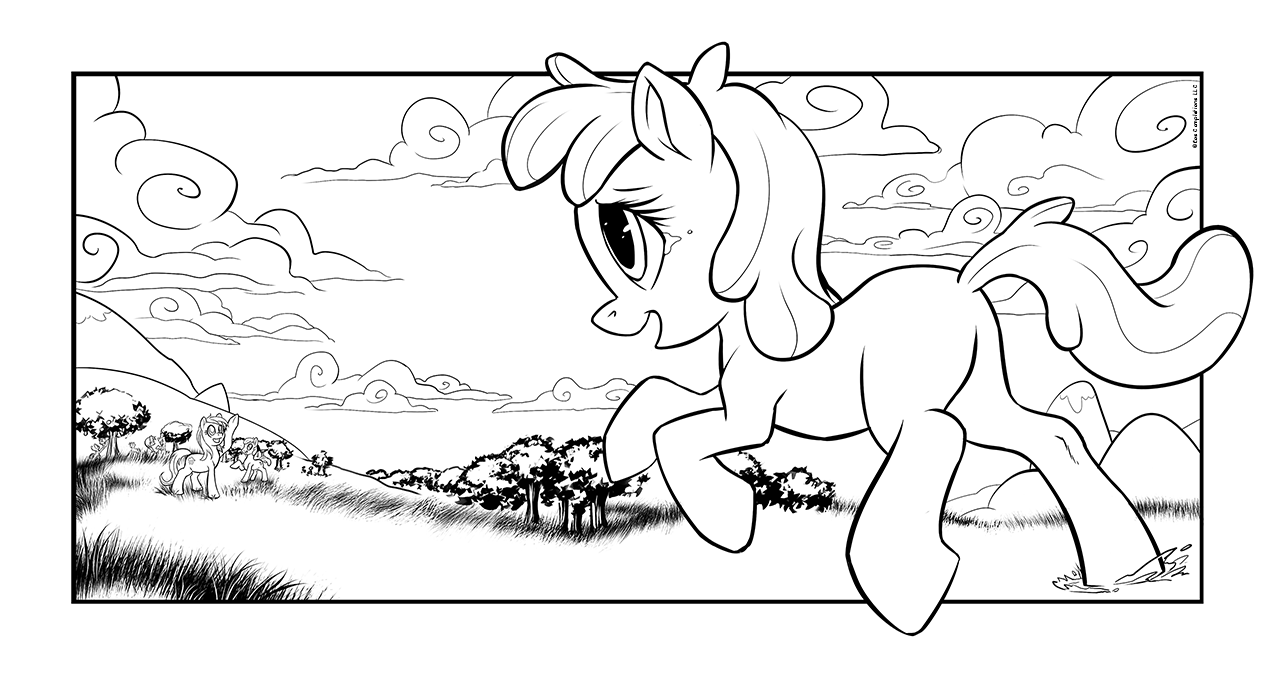
\includegraphics[width=0.9\linewidth]{image22.png}

\begin{motto}
    Do you believe in ghosts?
\end{motto}






\end{document}




